\documentclass{beamer}
\usepackage[T1]{fontenc}
\usepackage{multicol}
\usepackage{ragged2e}   %new code
\usepackage[utf8]{inputenc}
\usepackage[brazi	l]{varioref}
\usepackage[square,sort,comma,super,authoryear]{natbib}
\usepackage{xmpmulti}
\usepackage{verbatim}
\usepackage{epsfig}
\usepackage{subcaption}
\captionsetup{compatibility=false}
\usepackage{ru,graphicx,hyperref,url} % 
%\usepackage[pdftex]{hyperref}

\addtobeamertemplate{block begin}{}{\justifying}
\setbeamertemplate{section in toc}[sections numbered]
\AtBeginSection[]
{
  \begin{frame}{Conteúdo da Palestra}
  	\begin{multicols}{2}
      \tableofcontents[currentsection]
    \end{multicols}
  \end{frame}
}

% The title of the presentation:
%  - first a short version which is visible at the bottom of each slide;
%  - second the full title shown on the title slide;

\title[Backup e Restauração de Partições com CloneZilla]{
 Backup e Restauração de Partições com CloneZilla}

% Optional: a subtitle to be dispalyed on the title slide
% \subtitle{Show where you're from}

% The author(s) of the presentation:
%  - again first a short version to be displayed at the bottom;
%  - next the full list of authors, which may include contact information;
\author[\href{https://github.com/g1ll}{Gill Velleda Gonzales}]{
  Gill Velleda Gonzales\\
  \medskip
  {\small {\href{mailto:gillgonzales@ifsul.edu.br}{gillgonzales@ifsul.edu.br}}
  }}

% The institute:
%  - to start the name of the university as displayed on the top of each slide
%    this can be adjusted such that you can also create a Dutch version
%  - next the institute information as displayed on the title slide
\institute[TCHELINUX LIVRAMENTO 2019]{
 IFSUL - Campus Sant'ana do Livramento\\
  }

% Add a date and possibly the name of the event to the slides
%  - again first a short version to be shown at the bottom of each slide
%  - second the full date and event name for the title slide
\date{13 de Abril, 2019}

\begin{document}

\begin{comment}
\section{Título da Seção}
\subsection{Título da Subseção}
\begin{frame}
    \frametitle{\insertsection}
    \framesubtitle{\insertsubsection}
    \begin{block}{Título do Bloco}
   \justifying Texto da apresentação
    
    %FIGURA
    \begin{figure}
        \centering
        \includegraphics[scale=0.3]{img/fig1.png}
        \caption{Sintaxe para declaração de uma Função.}
    \end{figure}
    
    %ITENS
   	\begin{itemize}[<+-| alert@+>]
       \item Baixar a versão estável
       \item Preparar um pendrive
       \item Criar o pendrive de boot
    \end{itemize}
  \end{block}
\end{frame}
\end{comment}



\begin{frame}
  \titlepage
\end{frame}

\begin{frame}{Conteúdo da Palestra}
    \begin{multicols}{2}
    \tableofcontents
    \end{multicols}
\end{frame}

% Section titles are shown in at the top of the slides with the current section 
% highlighted. Note that the number of sections determines the size of the top 
% bar, and hence the university name and logo. If you do not add any sections 
% they will not be visible.
\section{Instalação}
\subsection{Download da ISO/ZIP}
\begin{frame}
    \frametitle{\insertsection}
    \framesubtitle{\insertsubsection}
    \justifying Entrar no site do Clonezilla  e baixar a ISO:
    
    \href{https://clonezilla.org/downloads/download.php?branch=stable}{https://clonezilla.org/downloads/download.php?branch=stable}
    
    \begin{itemize}[<+-| alert@+>]
        \item Baixar a versão estável (stable)
        \item Gravar a ISO em CD
        \item Criar um pendrive de boot
    \end{itemize}
\end{frame}
\begin{frame}
    \frametitle{\insertsection}
    \framesubtitle{\insertsubsection}
    
    %FIGURA
    \begin{figure}
        \centering
        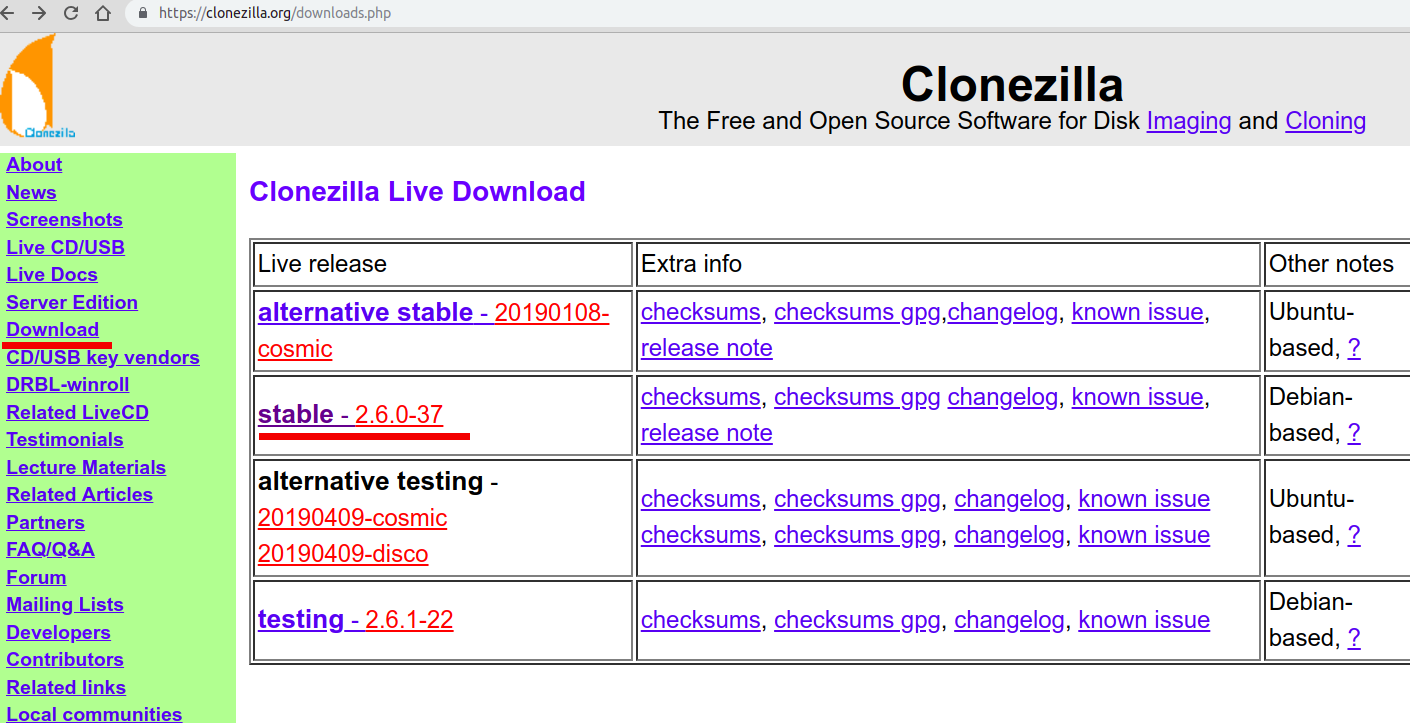
\includegraphics[scale=0.22]{images/baixando_clonezilla.png}
        \caption{Baixando a Versão Estável do Clonezilla na Web.}
    \end{figure}
\end{frame}

\begin{frame}
    \frametitle{\insertsection}
    \framesubtitle{\insertsubsection}
    
    %FIGURA
    \begin{figure}
        \centering
        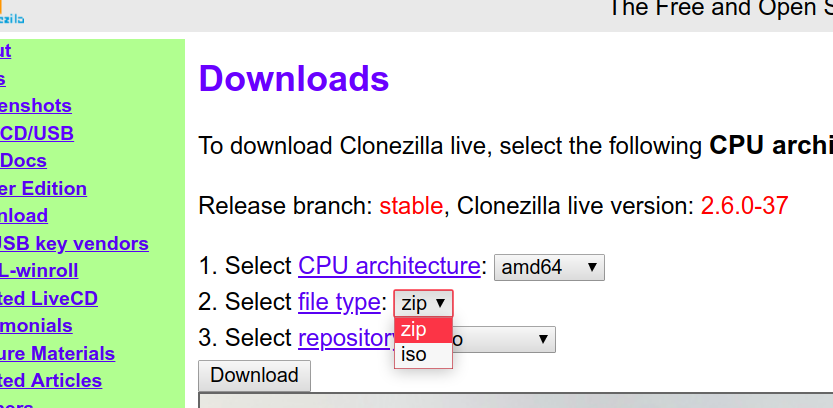
\includegraphics[scale=0.3]{images/baixando_clonezilla2.png}
        \caption{Baixando a Versão Estável do Clonezilla na Web.}
    \end{figure}
  
\end{frame}


\subsection{Pendrive de boot no Win}
\begin{frame}
 \frametitle{\insertsection}
    \framesubtitle{\insertsubsection}
     \begin{block}{\insertsubsection dows}
    \justifying Para preparar um pendrive inicializável do Clonezilla em ambiente windows, é preciso seguir os seguintes passos:
 
    \begin{itemize}[<+-| alert@+>]
        \item Formatar o pendrive para FAT32
        \item Extrair os arquivos do Clonezilla (ZIP)
        \item Rodar o makeboot.bat da pasta utils/sotype[win64]
    \end{itemize}
    \end{block}
\end{frame}

\begin{frame}
    \frametitle{\insertsection}
    \framesubtitle{\insertsubsection}
    
    %FIGURA
    \begin{figure}
        \centering
        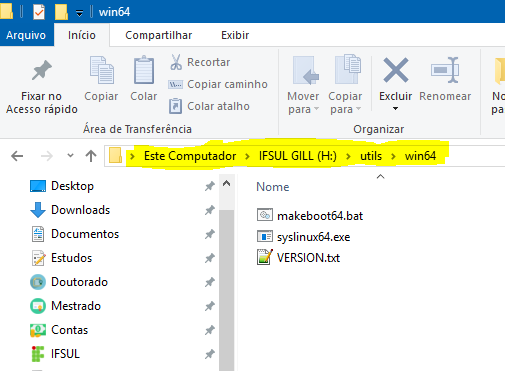
\includegraphics[scale=0.62]{images/pendrivewin_extraido.png}
        \caption{Criando o pendrive inicializável}
    \end{figure}
  
\end{frame}

\begin{frame}
    \frametitle{\insertsection}
    \framesubtitle{\insertsubsection}
    
    %FIGURA
    \begin{figure}
        \centering
        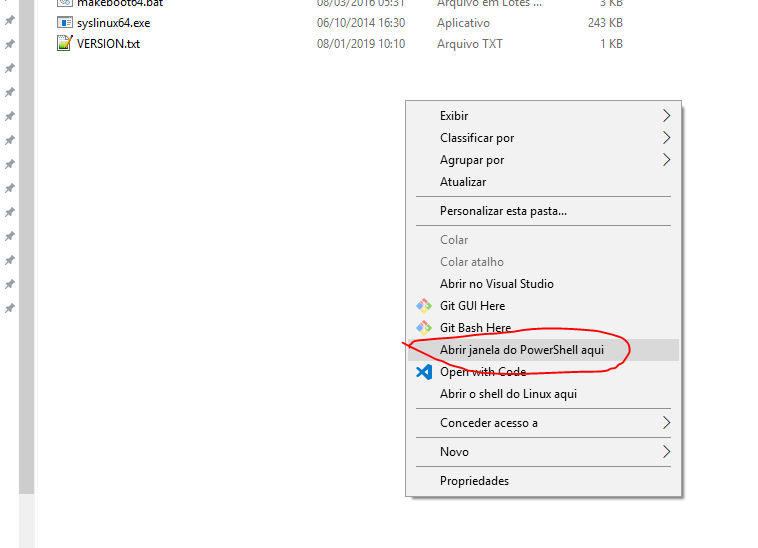
\includegraphics[scale=0.42]{images/pendrivewin1abrirpower.png}
        \caption{Abrir o PowerShell no diretório do pendrive utils/win64}
    \end{figure}
  
\end{frame}
\begin{frame}
    \frametitle{\insertsection}
    \framesubtitle{\insertsubsection}
      \begin{block}{\insertsubsection dows}
    \justifying Pressione a tecla SUPER(logo do Windows) + R e digite CMD
    \end{block}
    %FIGURA
    \begin{figure}
        \centering
        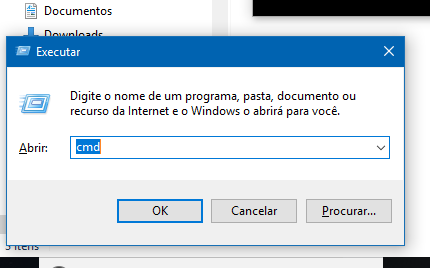
\includegraphics[scale=0.6]{images/pendrivewin2.png}
        \caption{Abrir o CMD e navegar até o diretório do pendrive utils/win64}
    \end{figure}
  
\end{frame}

\begin{frame}[plain,c]
    \frametitle{\insertsection}
    \framesubtitle{\insertsubsection}
    %FIGURA
    \begin{figure}
        \centering
        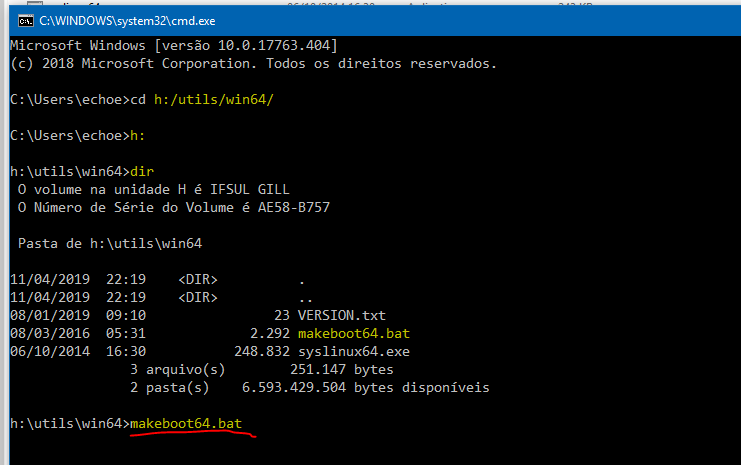
\includegraphics[scale=0.6]{images/pendrivewin3.png}
        \caption{Comandos para criar o pendrive de boot.}
    \end{figure}  
\end{frame}
\begin{frame}[plain,c]
    \frametitle{\insertsection}
    \framesubtitle{\insertsubsection}
    %FIGURA
    \begin{figure}
        \centering
        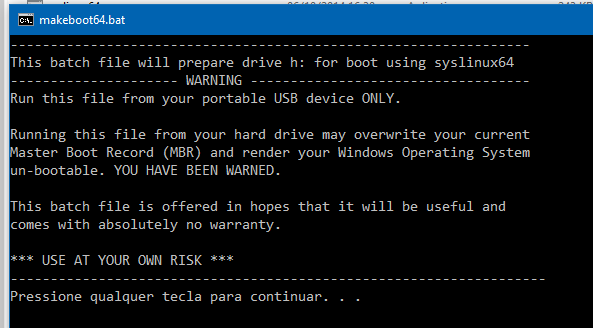
\includegraphics[scale=0.6]{images/pendrivewin4.png}
        \caption{Comandos para criar o pendrive de boot.}
    \end{figure}  
\end{frame}

\subsection{Pendrive de boot no Linux}
\begin{frame}
    \frametitle{\insertsection}
    \framesubtitle{\insertsubsection}
     \begin{block}{\insertsubsection }
    \justifying Para preparar um pendrive inicializável do Clonezilla em ambiente Linux, é preciso seguir os seguintes passos:
 
    \begin{itemize}[<+-| alert@+>]
        \item Formatar o pendrive para FAT32
        \item Extrair os arquivos do Clonezilla (ZIP)
        \item Rodar o makeboot.sh da pasta utils/linux
        \item Ou tornar o pendrive inicializável pelo GParted
        \item Ou rodar o USBCreator (Criador de disco de inicialização) e gravar a  ISO do Clonezilla
    \end{itemize}
    \end{block}
\end{frame}
\begin{frame}[plain,c]
    \frametitle{\insertsection}
    \framesubtitle{\insertsubsection}
    %FIGURA
    \begin{figure}
        \centering
        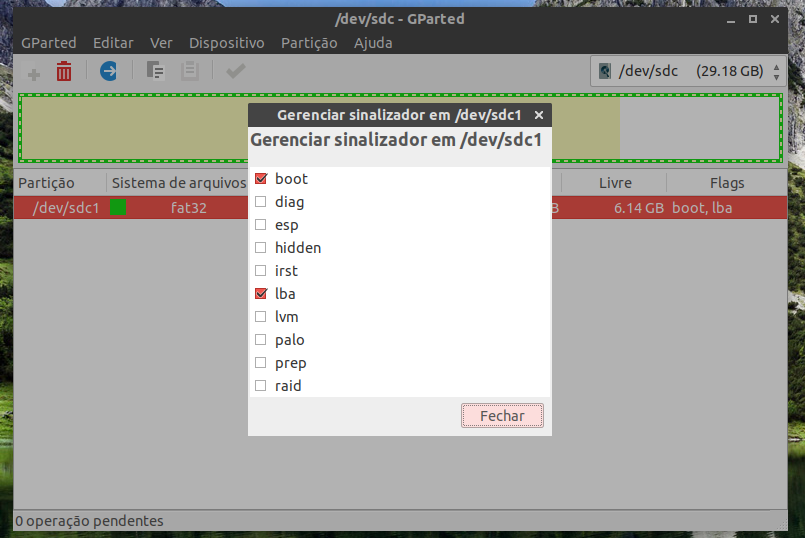
\includegraphics[scale=0.4]{images/pendrivebootavellinux.png}
        \caption{Comandos para criar o pendrive de boot no Linux.}
    \end{figure}  
\end{frame}

\section{Partições de Disco no Linux}
\subsection{Nomes de Partições}
\begin{frame}
    \frametitle{\insertsection}
    \framesubtitle{\insertsubsection}
     \begin{block}{\insertsubsection}
  	\justifying
  O Clonezilla é um sistema baseado em Linux, distribuição Debian, e as partições de disco são identificadas pela nomenclatura do sistema Linux.
   
   \begin{itemize}[<+-| alert@+>]
        \item SDA nome do disco A
        \item SDB nome do disco B
        \item SDA1 nome da partição 1 do disco A
        \item SDA2 nome da partição 2 do disco A
        \item SDB1 nome da partição 1 do disco B
    \end{itemize}
\end{block}
\end{frame}
\begin{frame}[plain,c]
    \frametitle{\insertsection}
    \framesubtitle{\insertsubsection}
    %FIGURA
    \begin{figure}
        \centering
        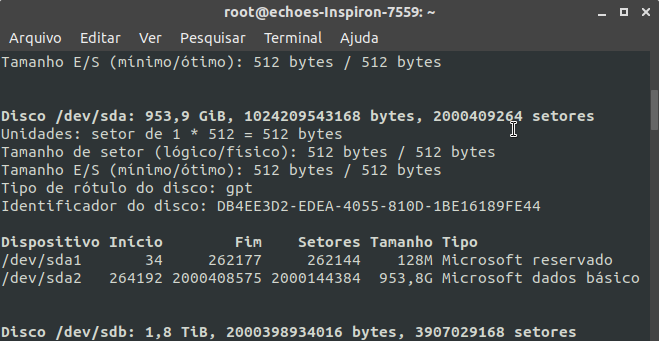
\includegraphics[scale=0.6]{images/discos1.png}
        \caption{Saída do comando fdisk -l para disco SDA.}
    \end{figure}  
\end{frame}
\begin{frame}[plain,c]
    \frametitle{\insertsection}
    \framesubtitle{\insertsubsection}
    %FIGURA
    \begin{figure}
        \centering
        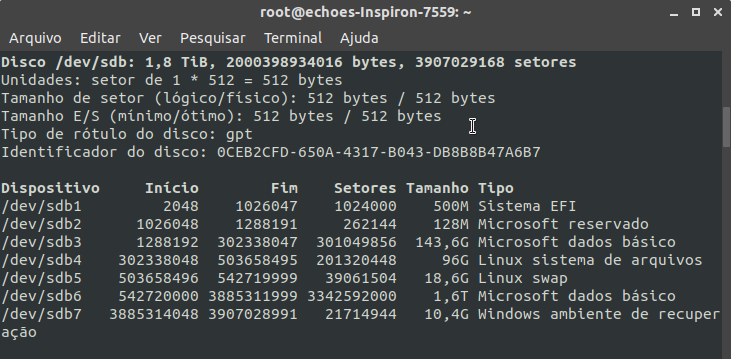
\includegraphics[scale=0.6]{images/disco2.png}
        \caption{Saída do comando fdisk -l para disco SDB.}
    \end{figure}  
\end{frame}
\begin{frame}[plain,c]
    \frametitle{\insertsection}
    \framesubtitle{\insertsubsection}
    %FIGURA
    \begin{figure}
        \centering
        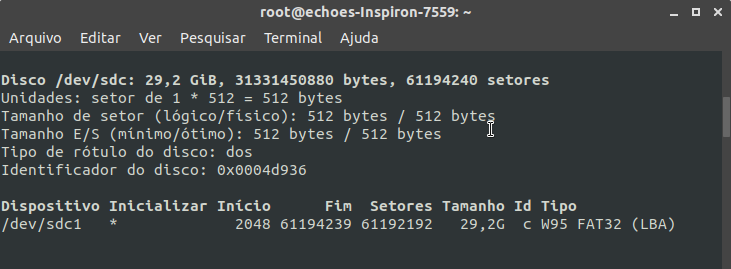
\includegraphics[scale=0.6]{images/disco3.png}
        \caption{Saída do comando fdisk -l para disco SDC.}
    \end{figure}  
\end{frame}

\subsection{Sistemas de Arquivos}
\begin{frame}[plain,c]
   \frametitle{\insertsection}
    \framesubtitle{\insertsubsection}
    \begin{figure}
        \centering
        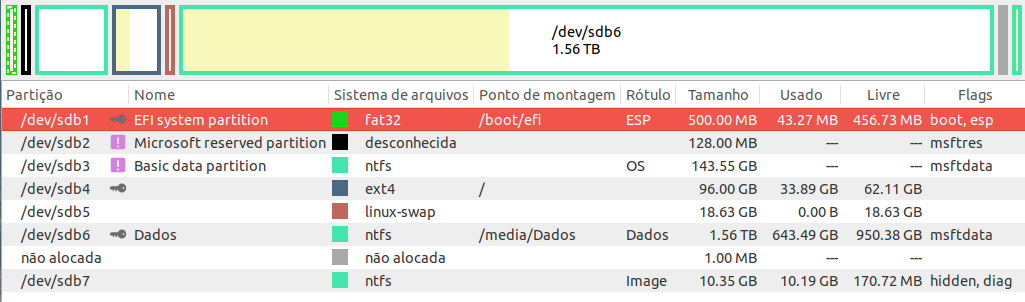
\includegraphics[width=2.1\linewidth]{images/particoes.png}
        \caption{Partições no Linux Programa GParted}
    \end{figure}
\end{frame}

\begin{frame}[plain,c]
   \frametitle{\insertsection}
    \framesubtitle{\insertsubsection}
    \begin{figure}
        \centering
        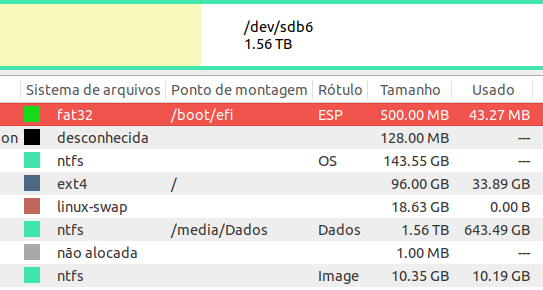
\includegraphics[width=1.3\linewidth]{images/particoes2.png}
        \caption{Partições no Linux Programa GParted}
    \end{figure}
\end{frame}


\section{Backup de Partições}
\subsection{Tutorial de Backup de uma Partição}
\begin{frame}
    \frametitle{\insertsection}
    \framesubtitle{\insertsubsection}
     \begin{block}{\insertsubsection}
  	\justifying
 Para fazer o backup, ou melhor a CÓPIA, criando uma IMAGEM da sua partição precisamos:
   
   \begin{itemize}[<+-| alert@+>]
        \item Dar boot do pendrive com o CLONEZILLA 
        \item Inicializar a partir do pendrive (F2,F12,F8,F9, dependendo da BIOS da placa-mãe)
        \item Saber identificar a partição de origem (SDA1, SDB1 etc...) 
        \item Ter uma partição de DESTINO para salvar o arquivo de IMAGEM da partição
        \item Ter espaço suficiente na partição de DESTINO
        \item DESTINO pode ser outra PARTIÇÃO DO MESMO HD ou PARTIÇÃO de OUTRO HD ou HD Externo
    \end{itemize}
\end{block}
\end{frame}

\begin{frame}[plain,c]
   \frametitle{\insertsection}
    \framesubtitle{Inicializando pelo pendrive}
    \begin{figure}[!h]
        
        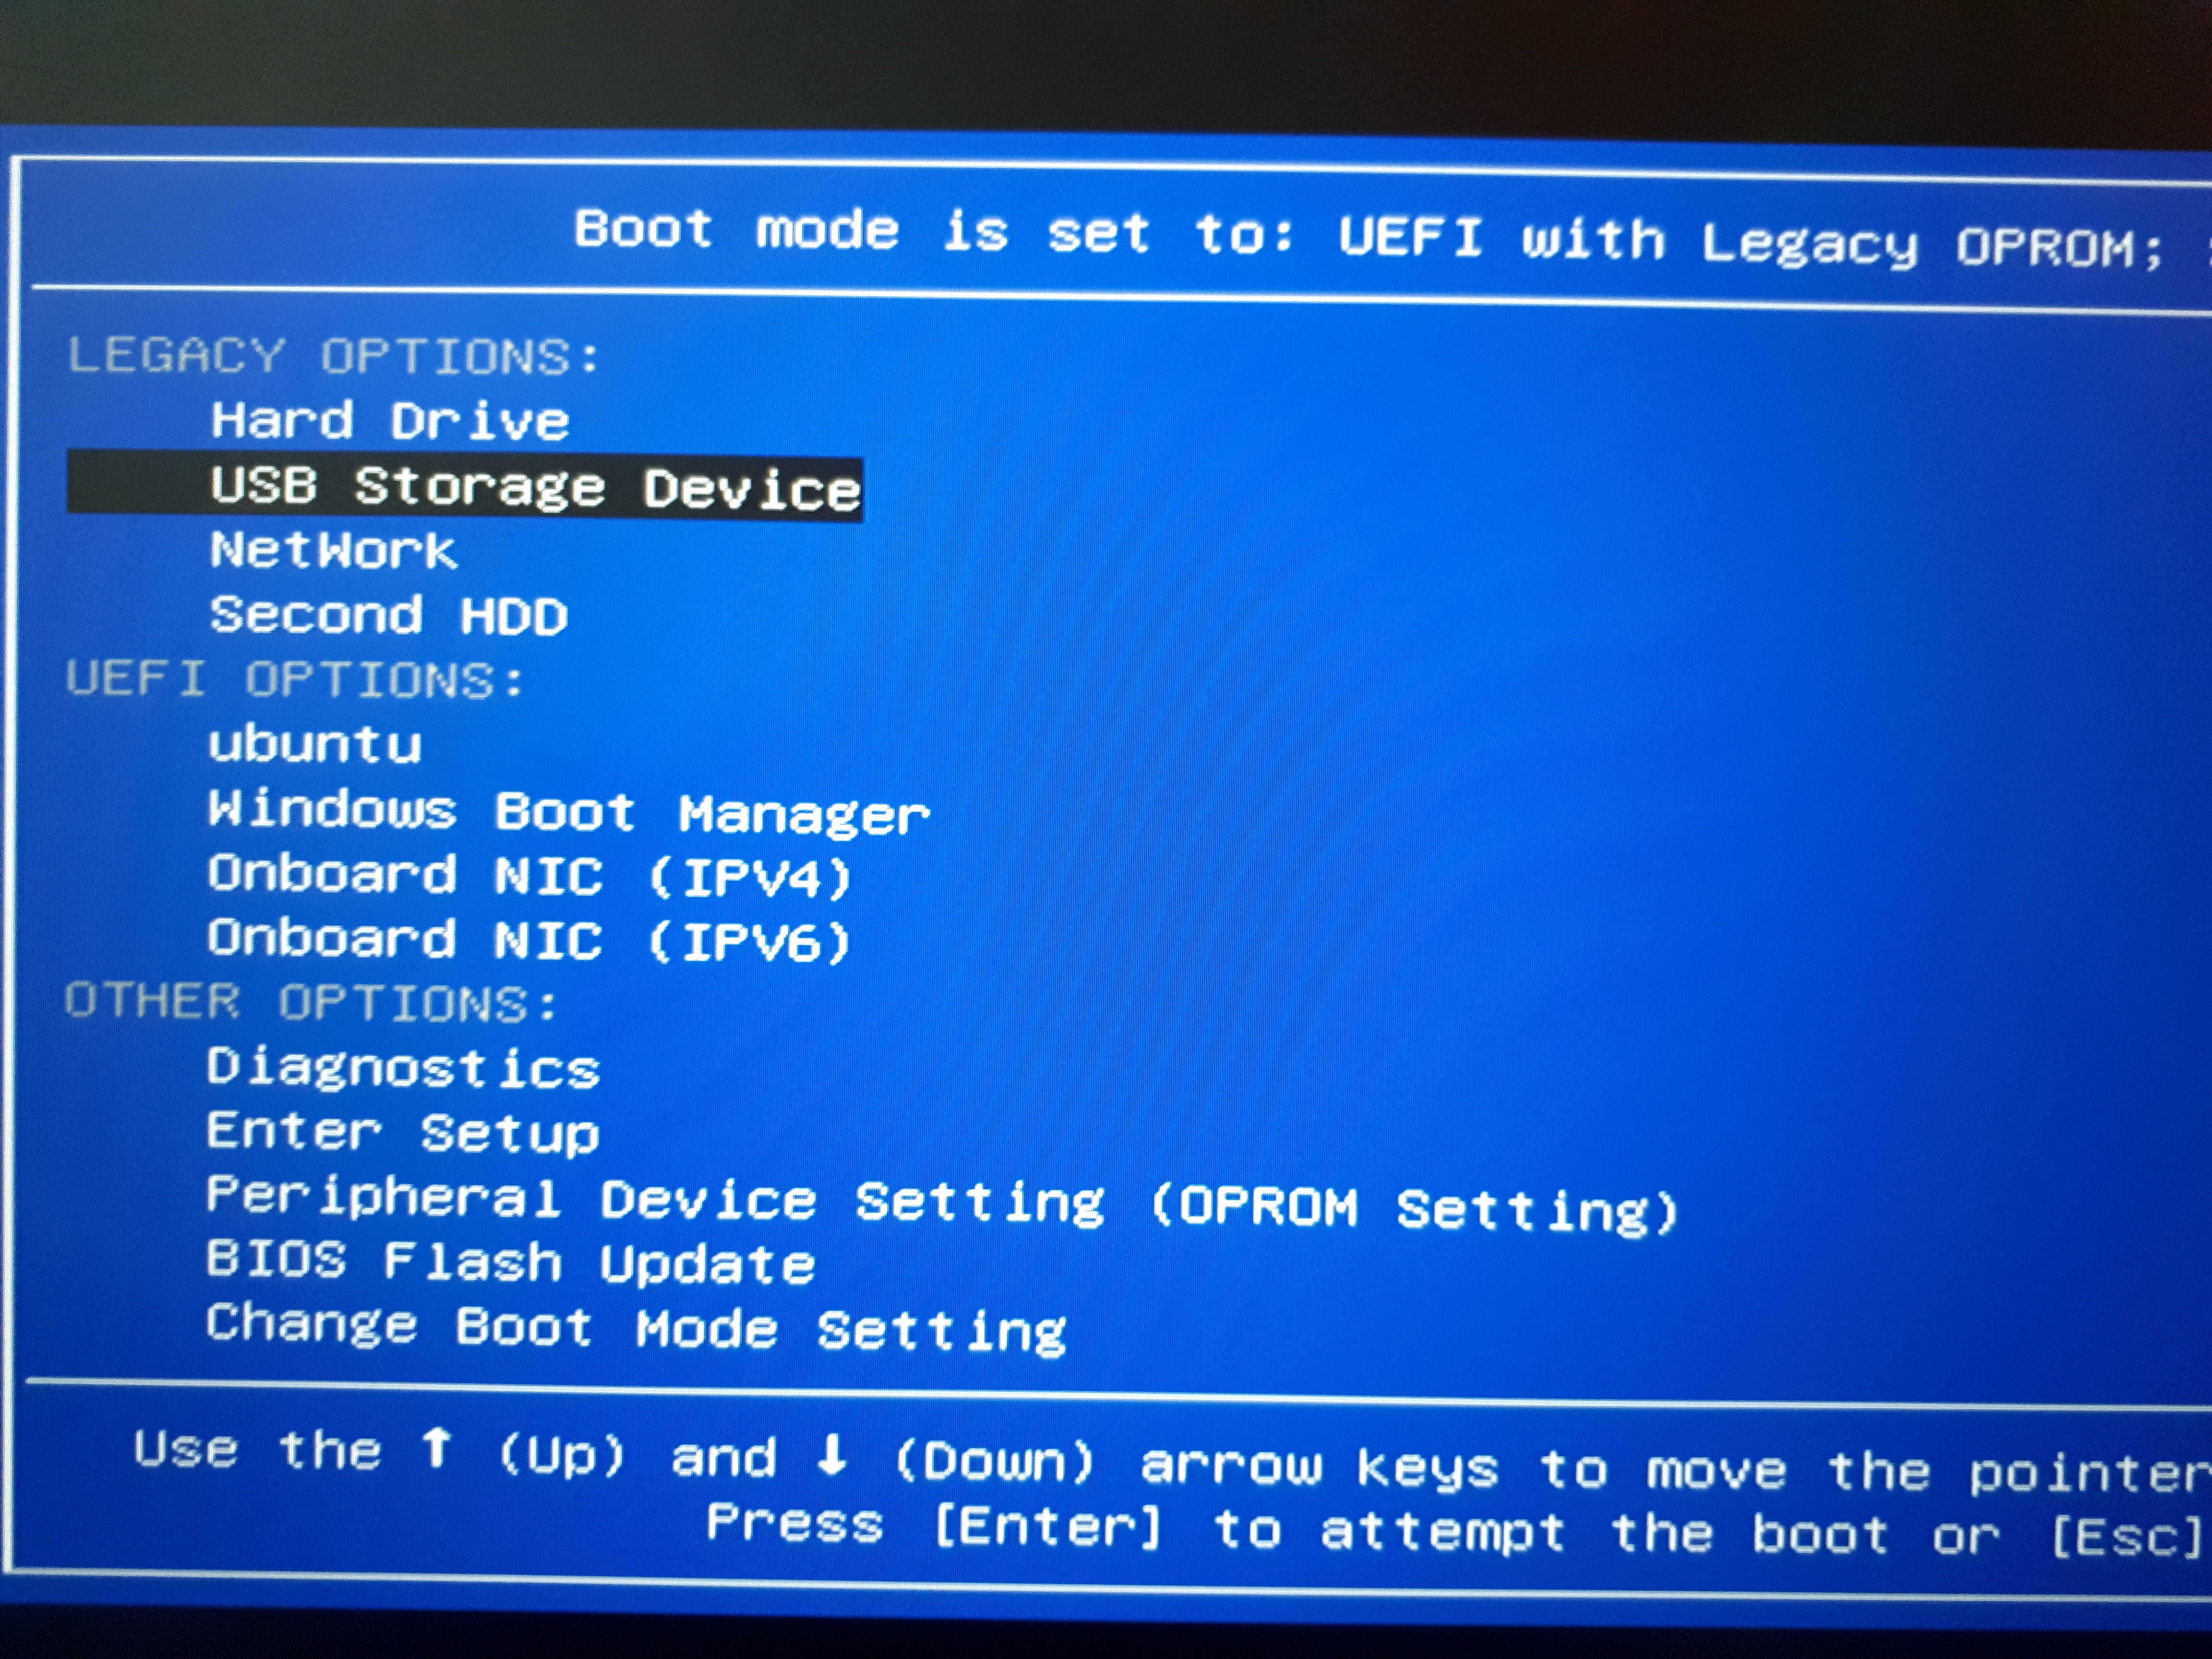
\includegraphics[width=1\linewidth]{images/backup/bkp1.jpg}
        \caption{Partições no Linux Programa GParted}
    \end{figure}
\end{frame}

\begin{frame}[plain,c]
   \frametitle{\insertsection}
    \framesubtitle{Tela inicial do CloneZilla}
    \begin{figure}[!h]
        
        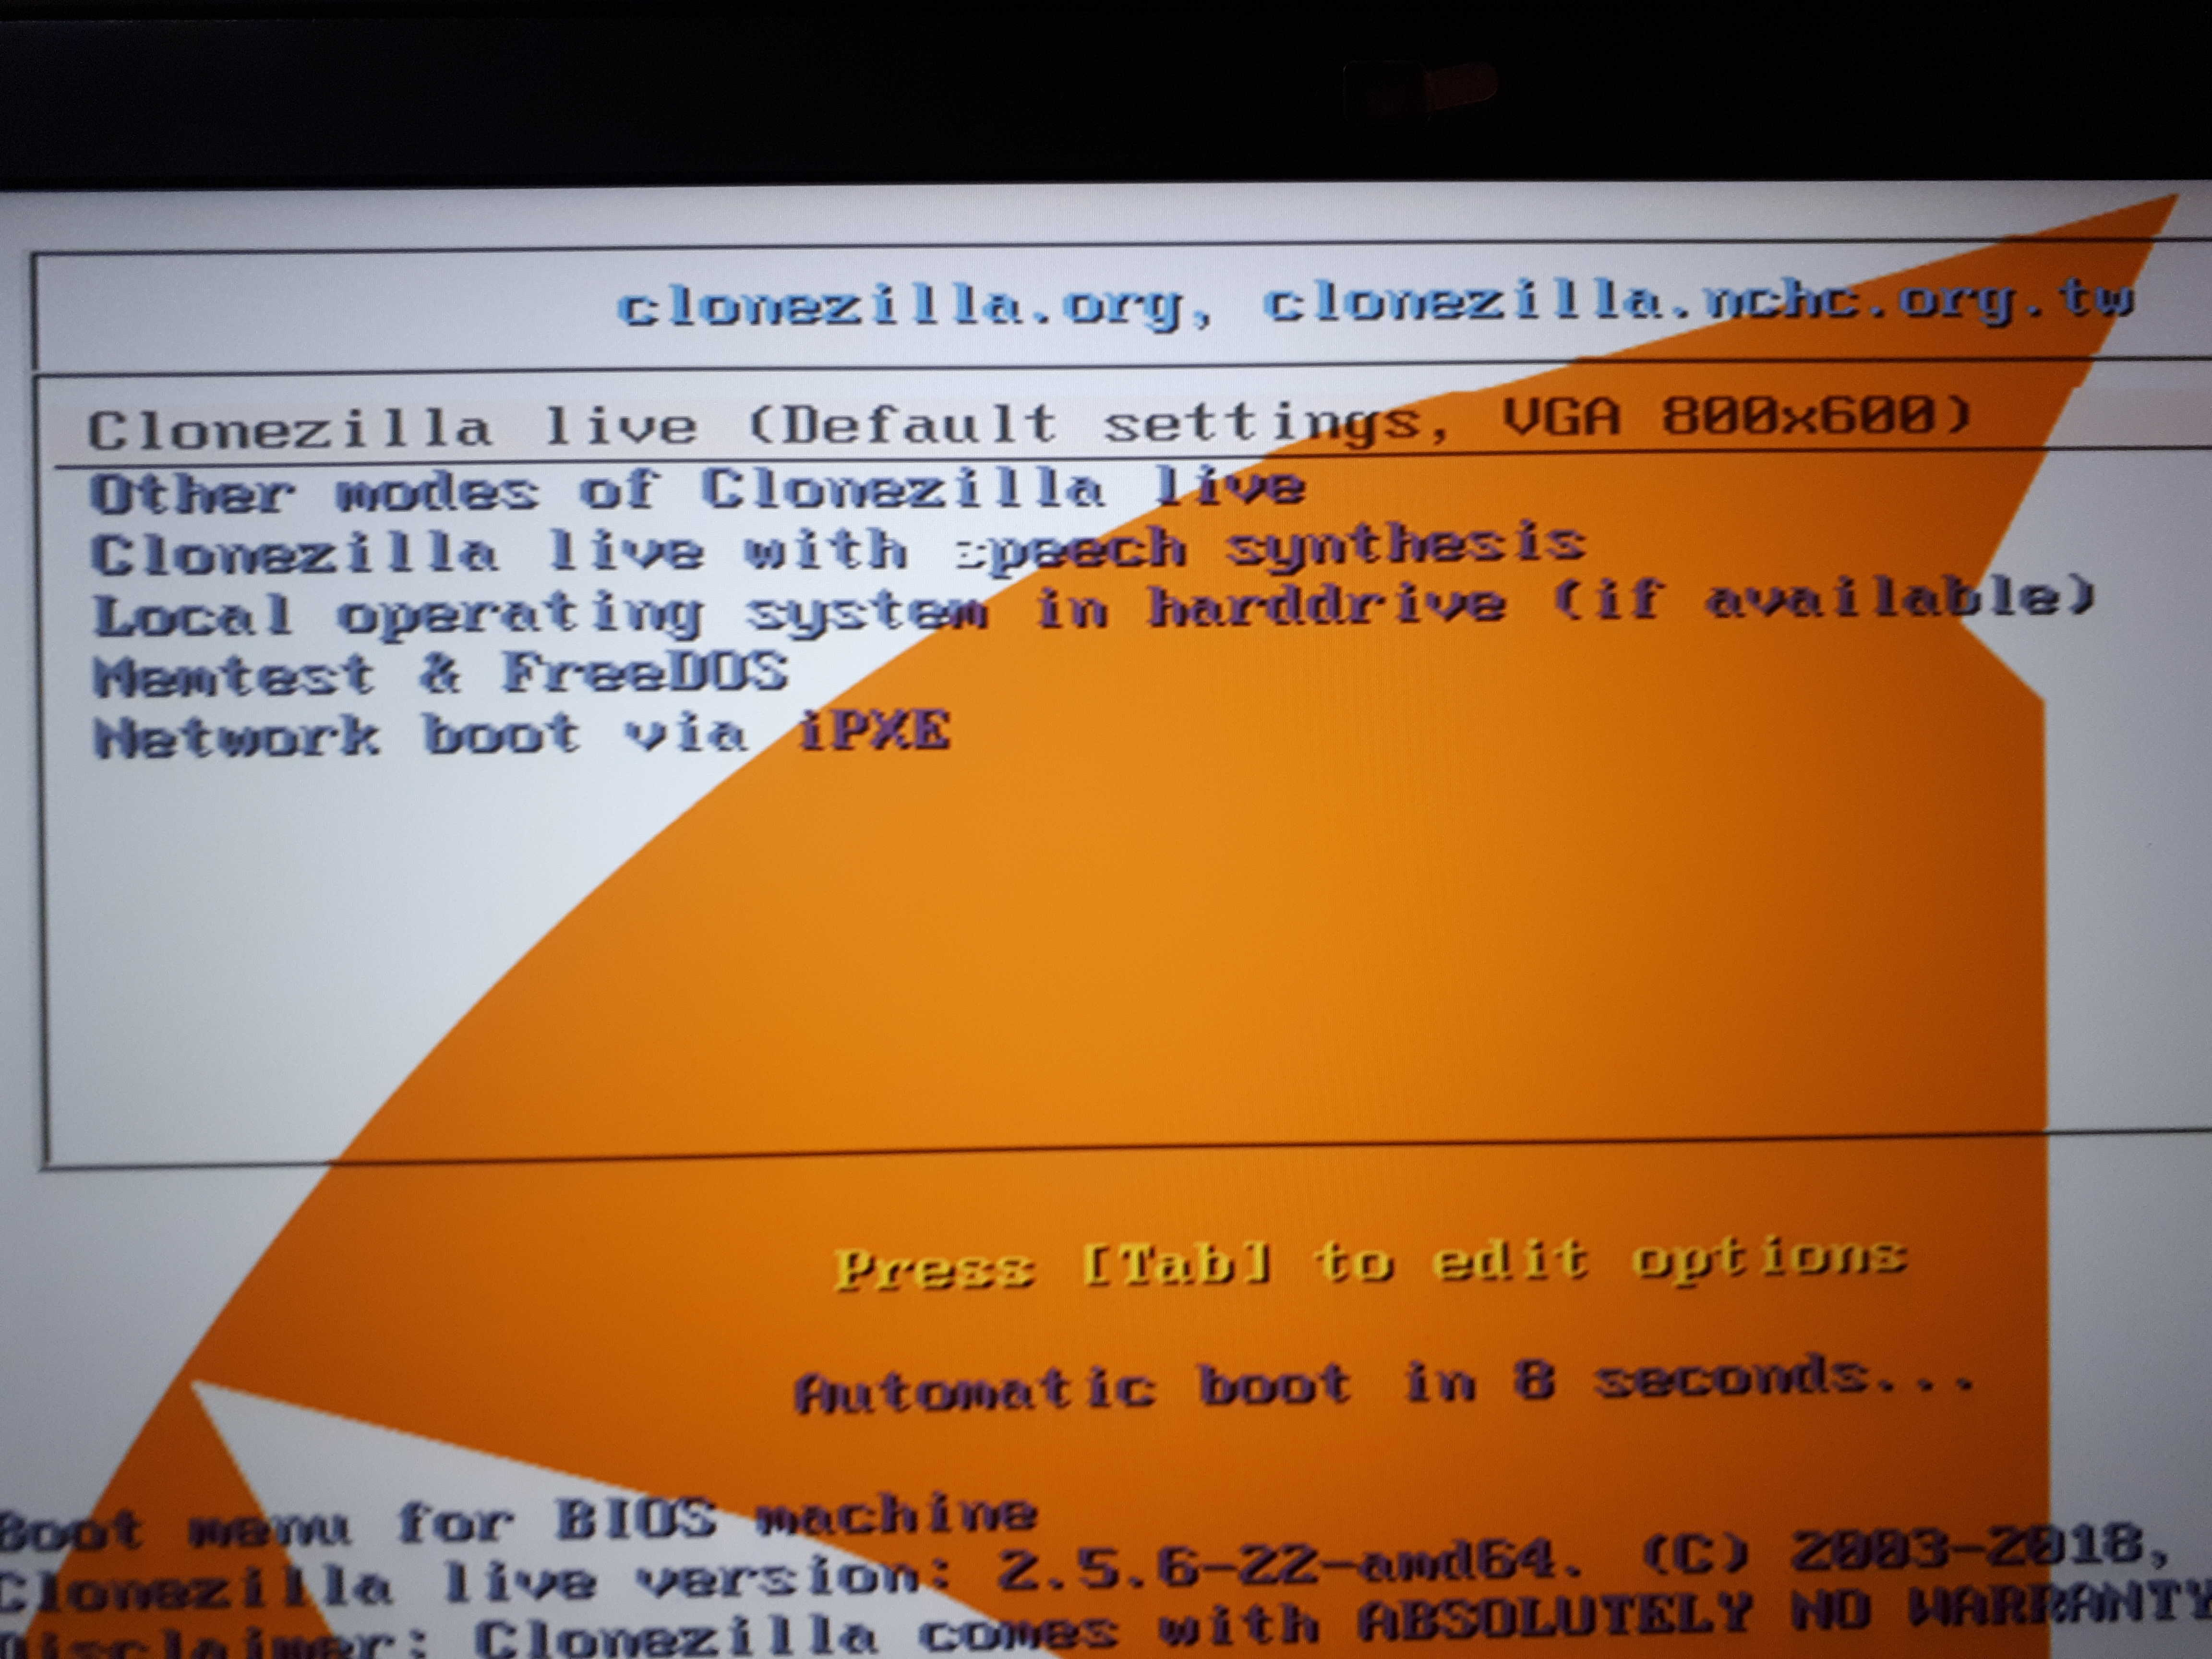
\includegraphics[width=1\linewidth]{images/backup/bkp2.jpg}
        \caption{Partições no Linux Programa GParted}
    \end{figure}
\end{frame}

\begin{frame}[plain,c]
   \frametitle{\insertsection}
    \framesubtitle{Escolhendo Idioma}
    \begin{figure}[!h]
        
        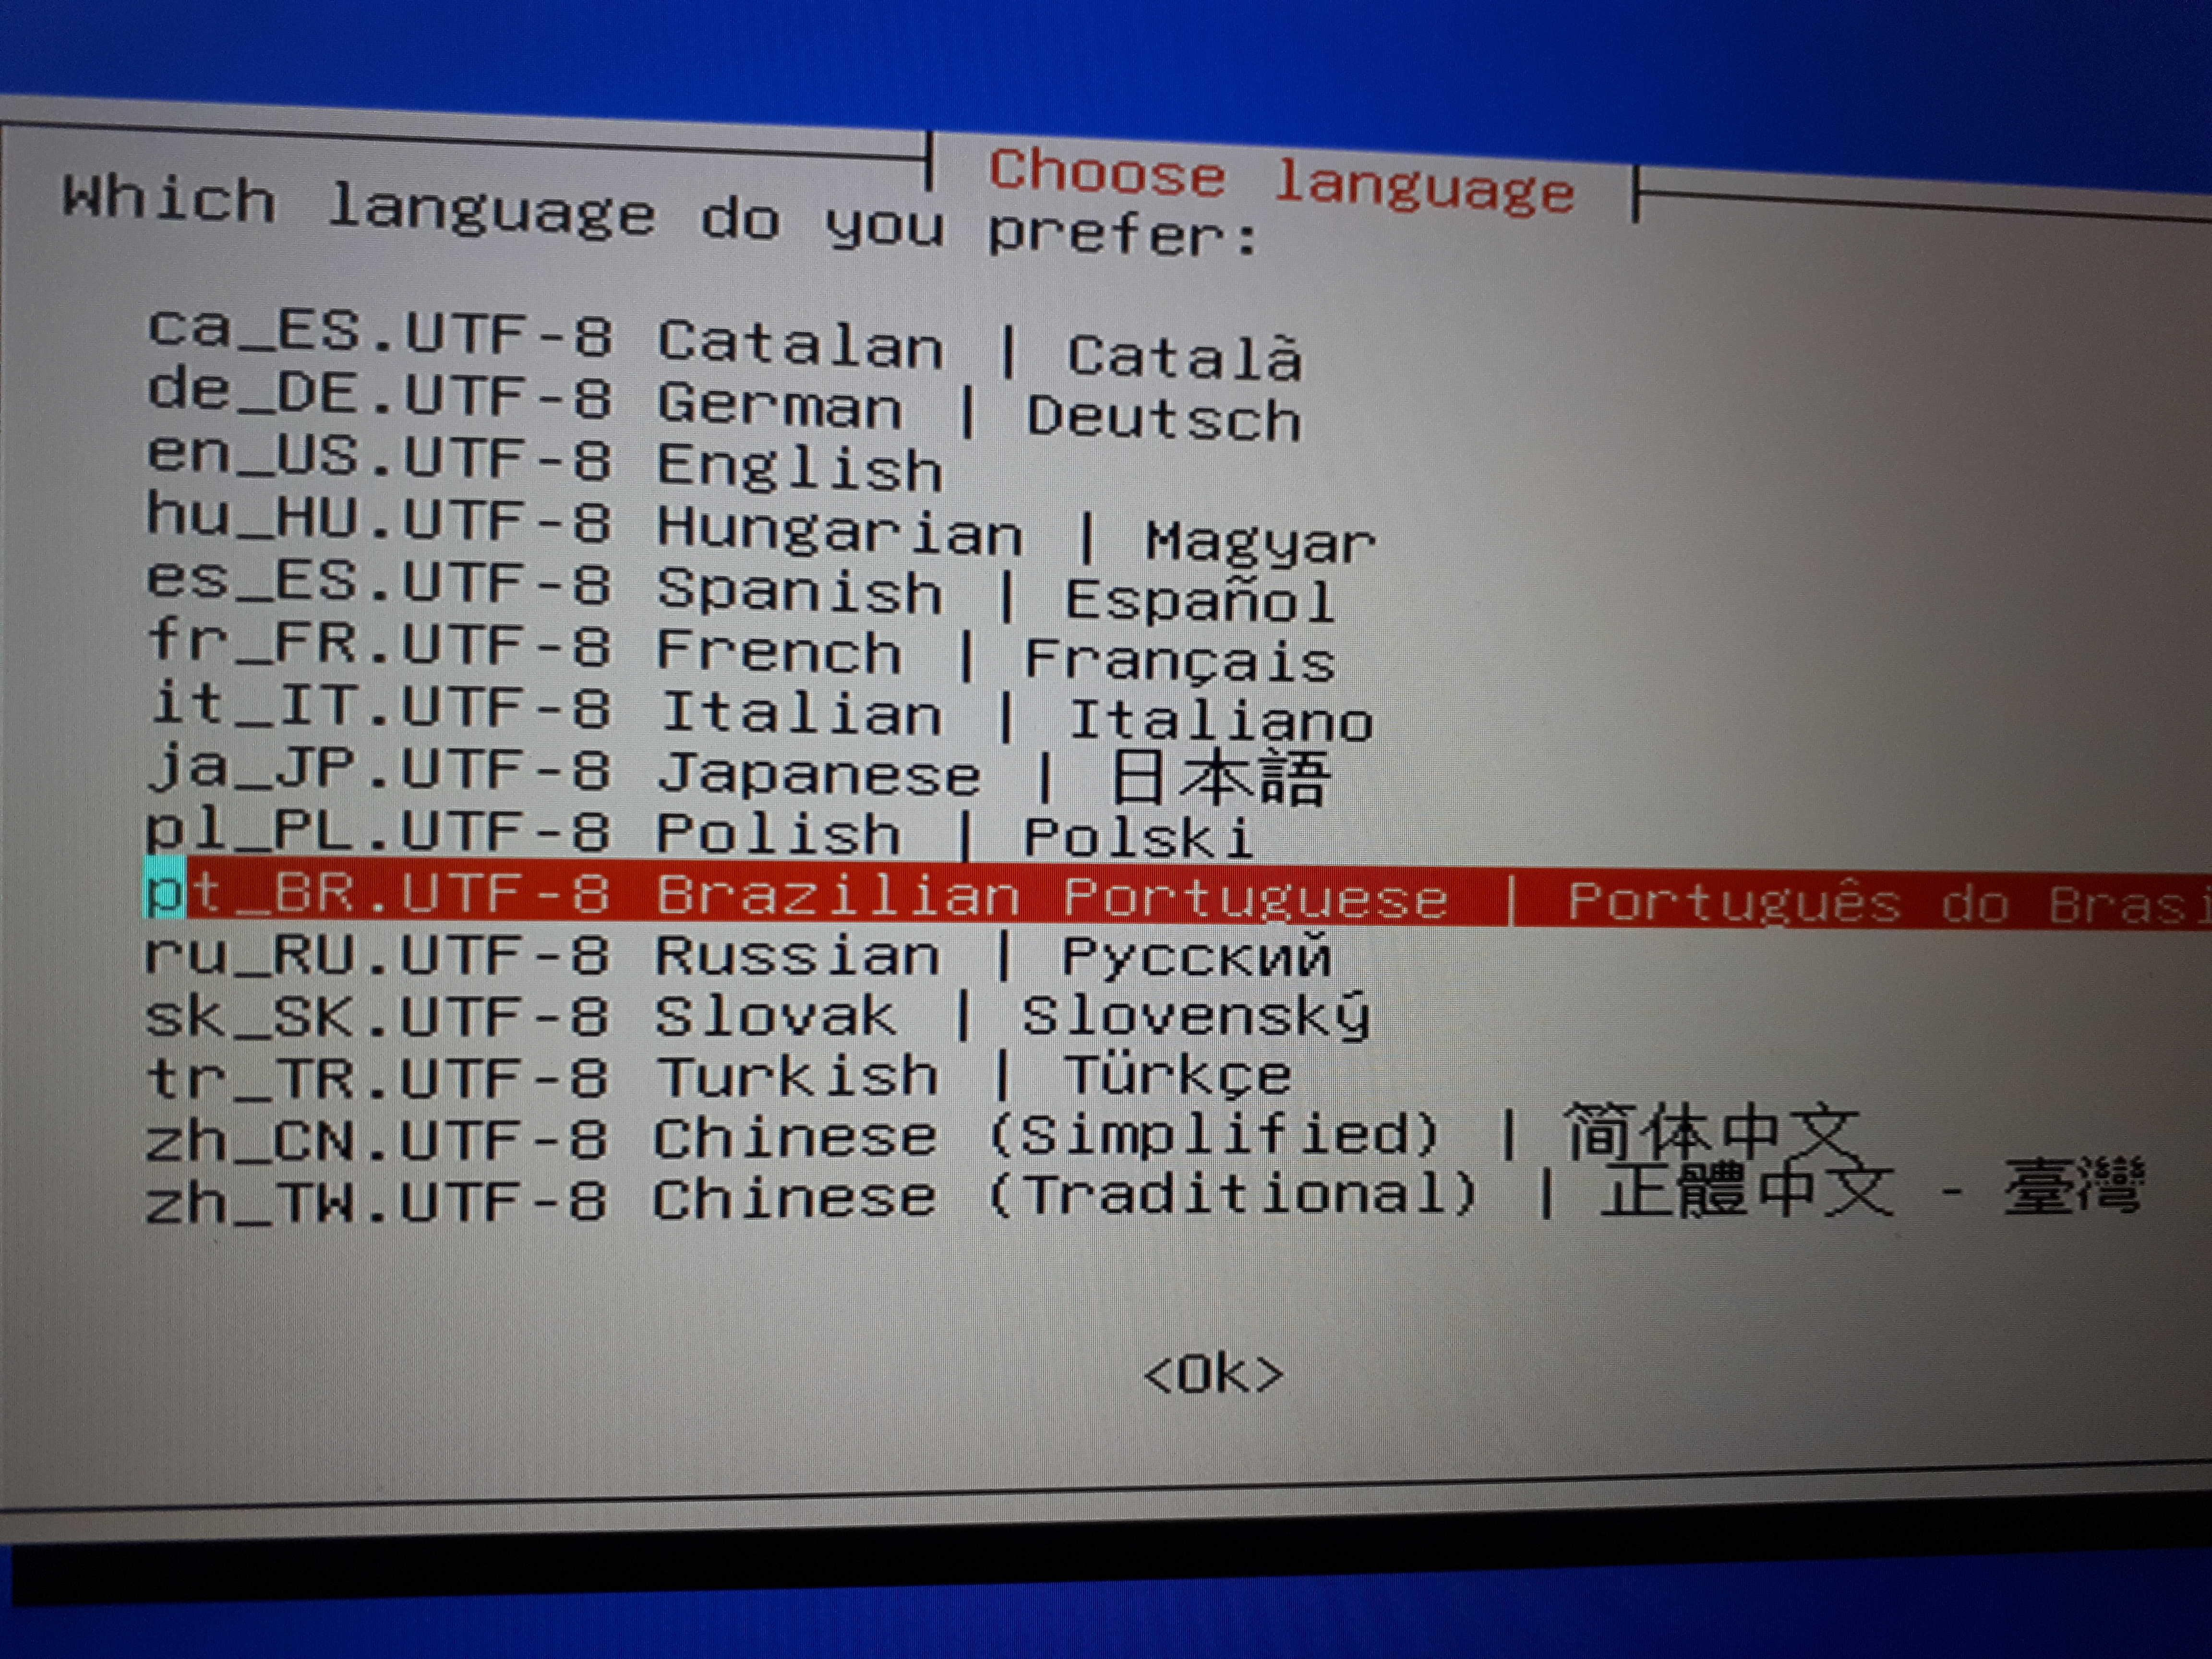
\includegraphics[width=1\linewidth]{images/backup/bkp3.jpg}
        \caption{Partições no Linux Programa GParted}
    \end{figure}
\end{frame}

\begin{frame}[plain,c]
   \frametitle{\insertsection}
    \framesubtitle{Layout do Teclado}
    \begin{figure}[!h]
        
        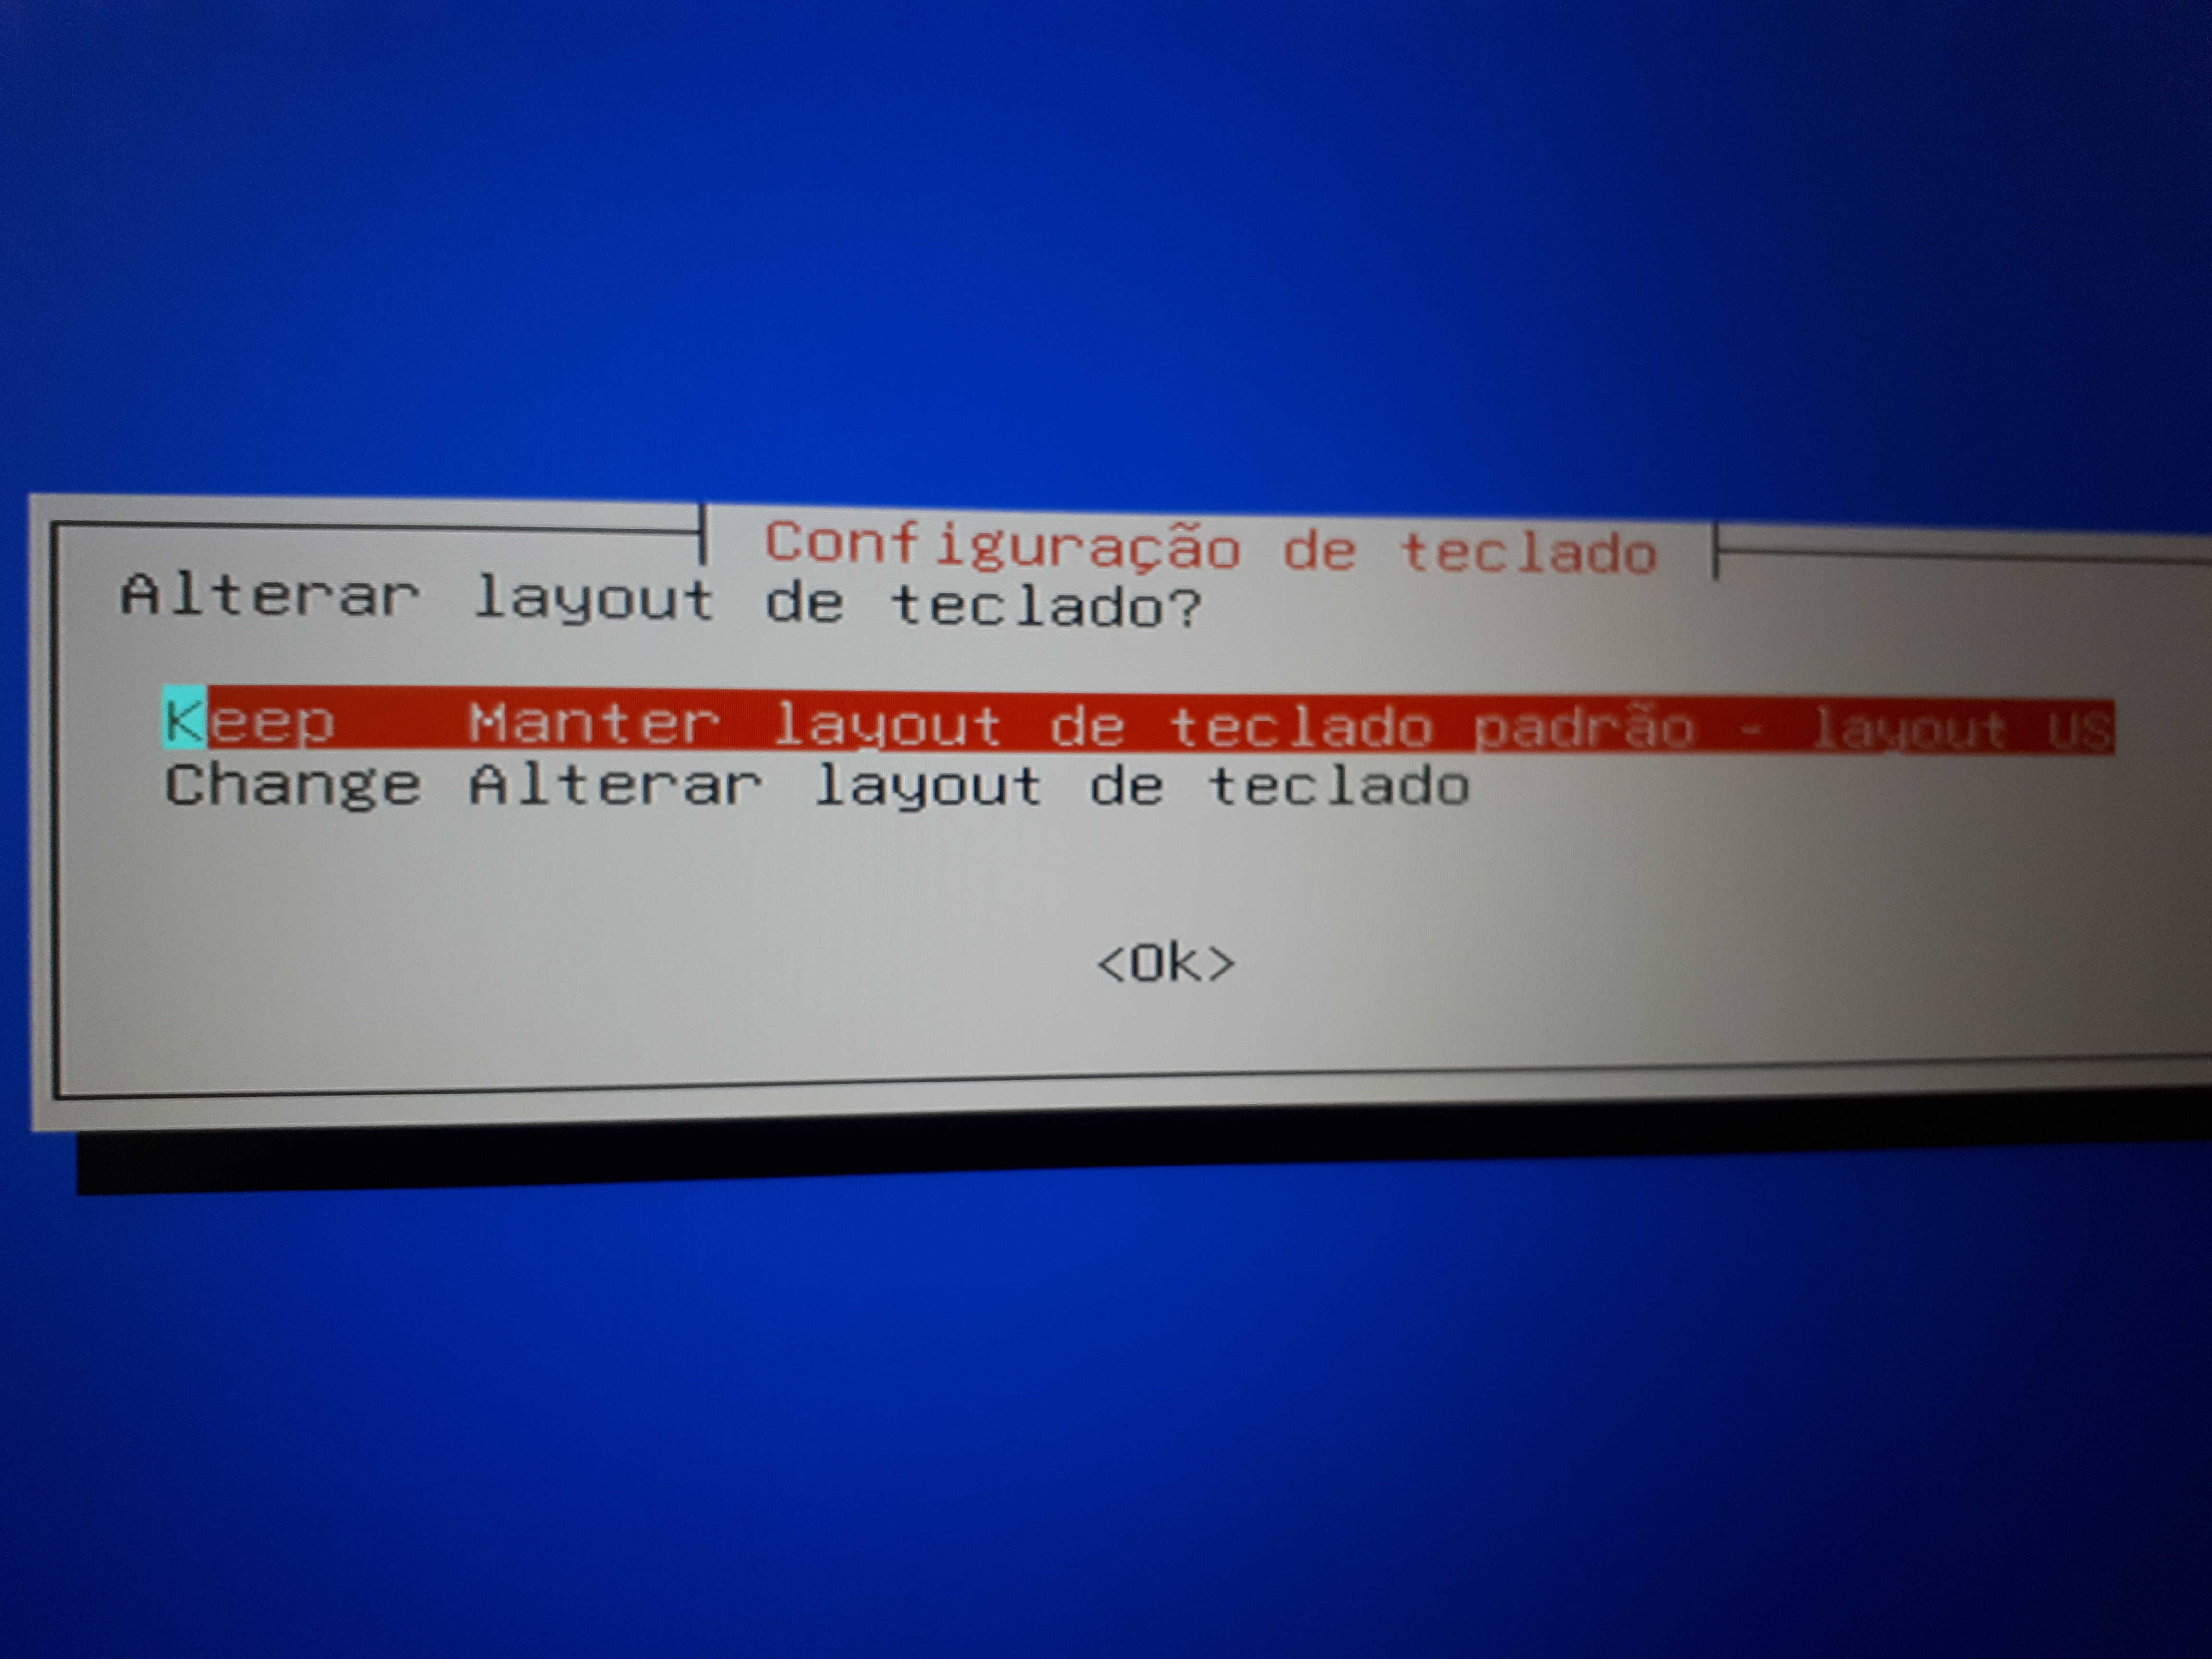
\includegraphics[width=1\linewidth]{images/backup/bkp4.jpg}
        \caption{Partições no Linux Programa GParted}
    \end{figure}
\end{frame}

\begin{frame}[plain,c]
   \frametitle{\insertsection}
    \framesubtitle{Iniciar CloneZilla}
    \begin{figure}[!h]
        
        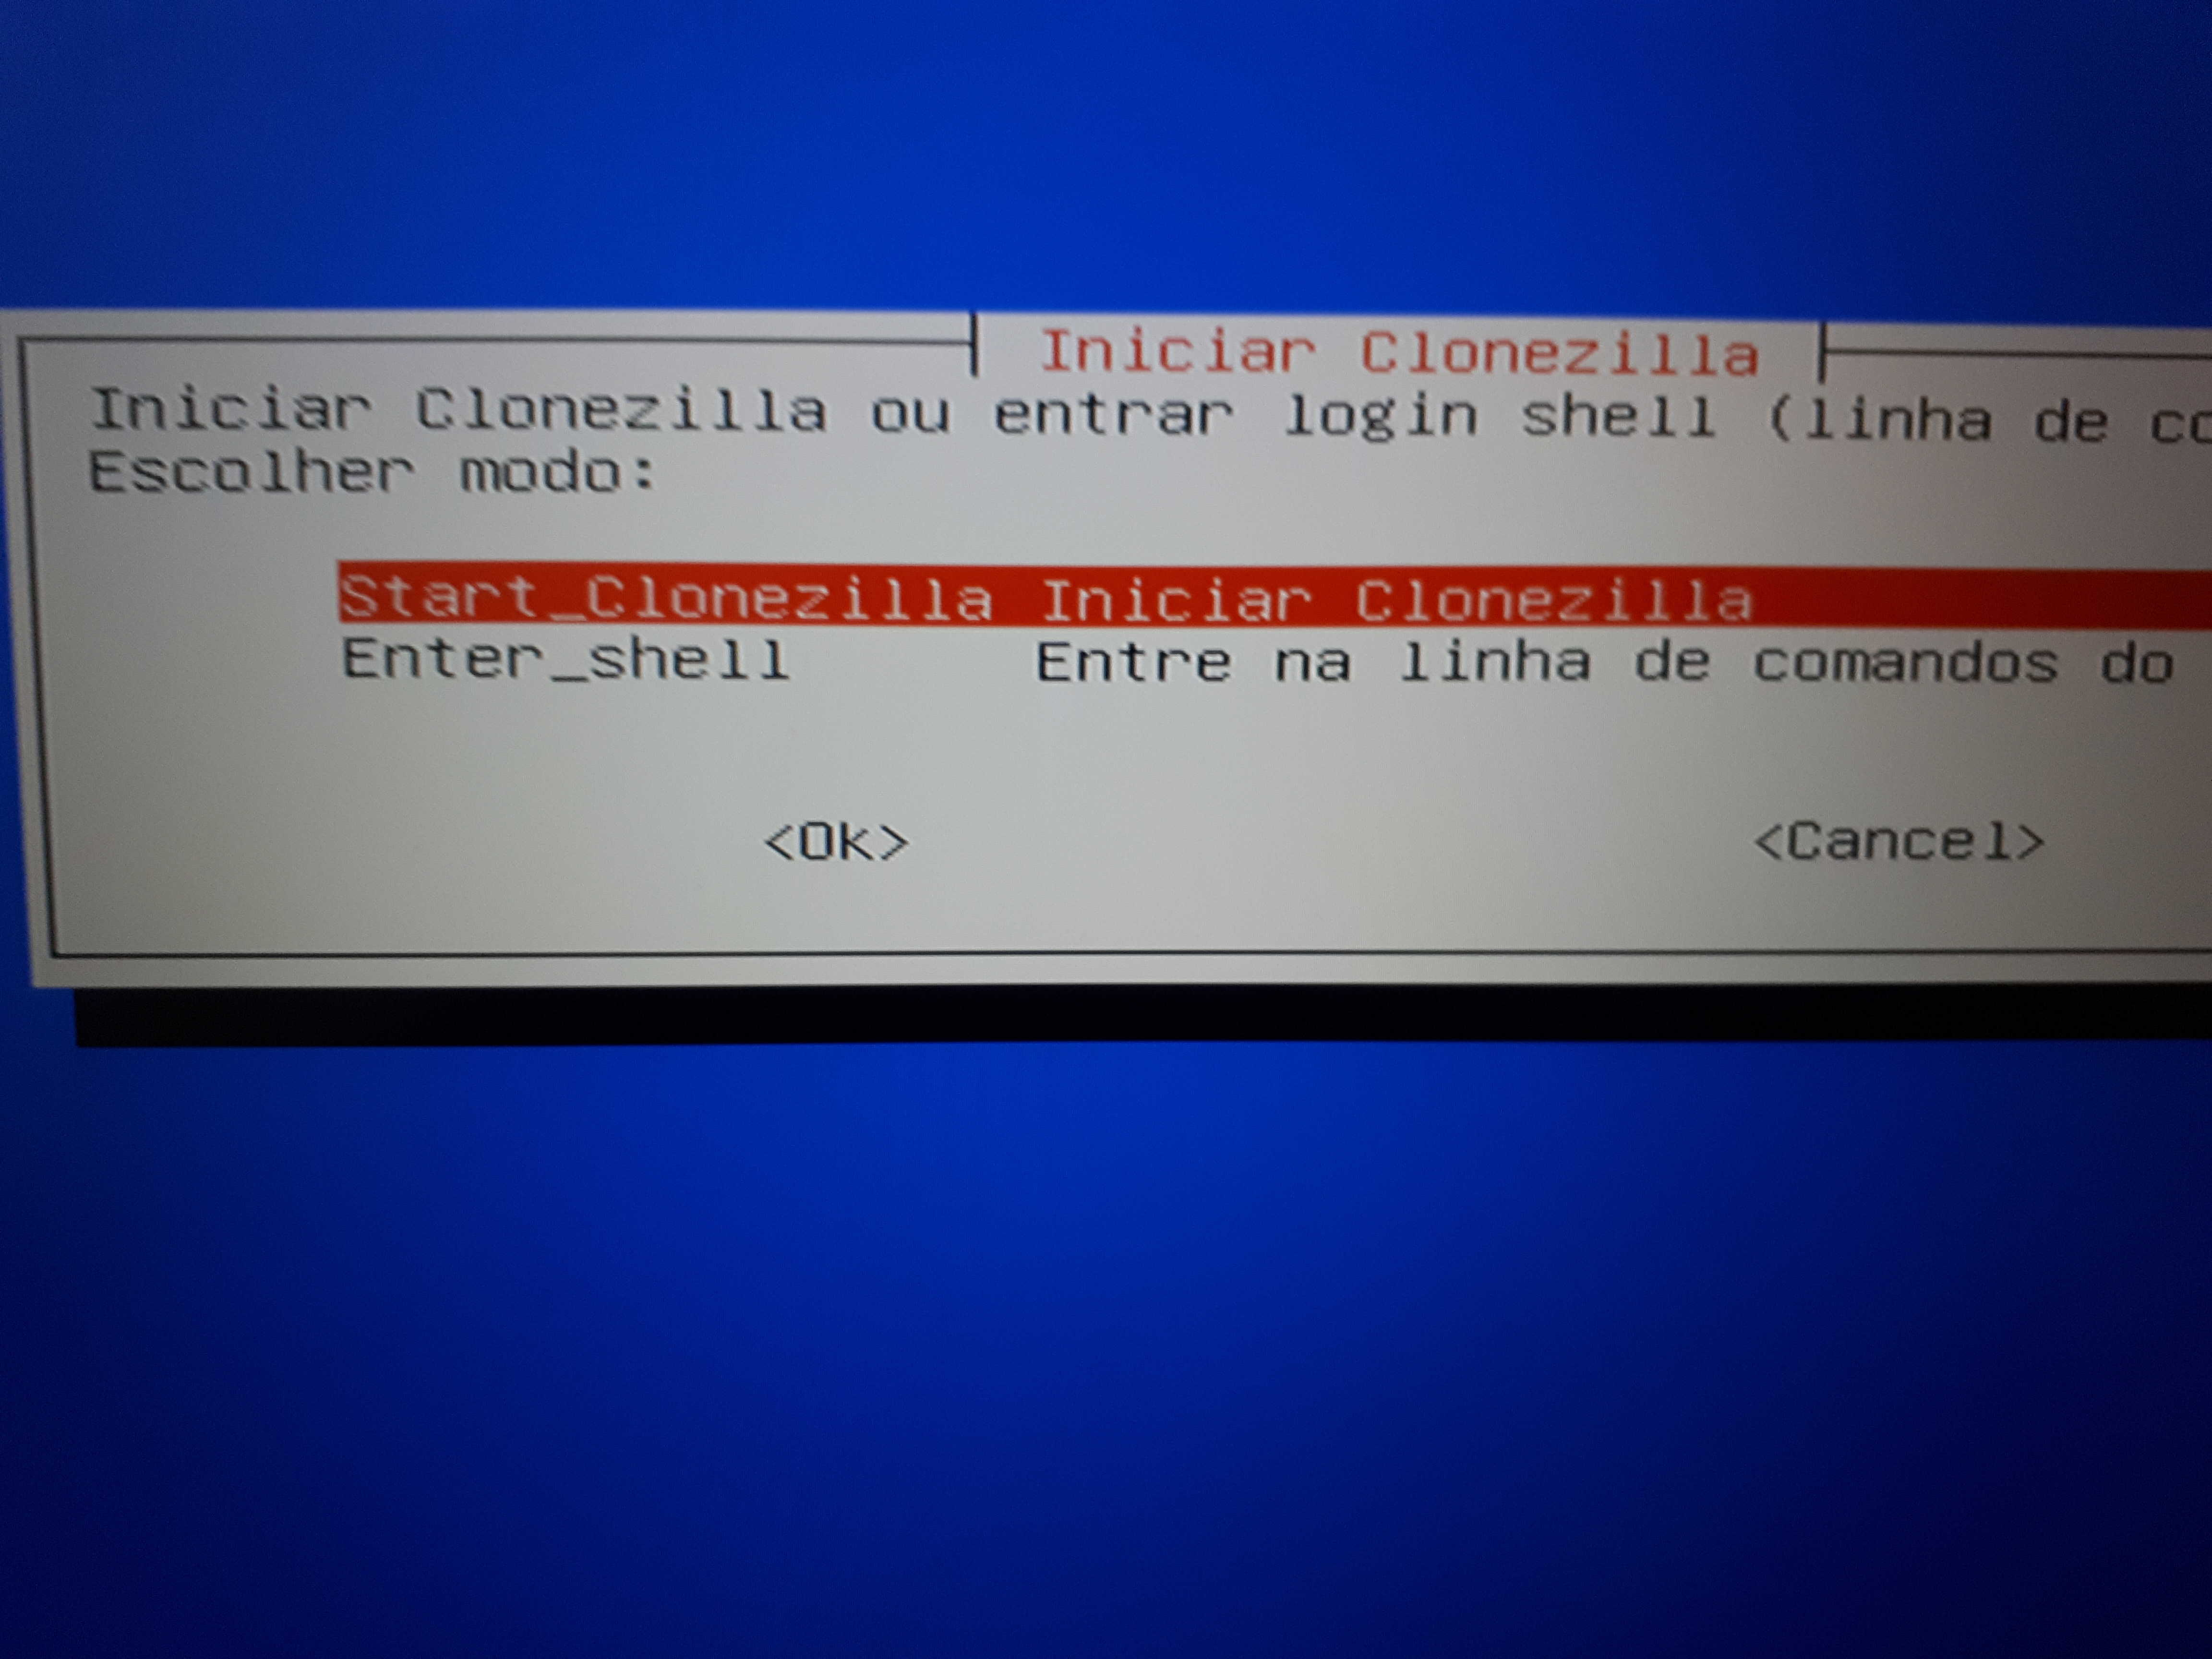
\includegraphics[width=1\linewidth]{images/backup/bkp5.jpg}
        \caption{Partições no Linux Programa GParted}
    \end{figure}
\end{frame}


\begin{frame}[plain,c]
   \frametitle{\insertsection}
    \framesubtitle{Escolher DISCO/PARTIÇÃO}
    \begin{figure}[!h]
        
        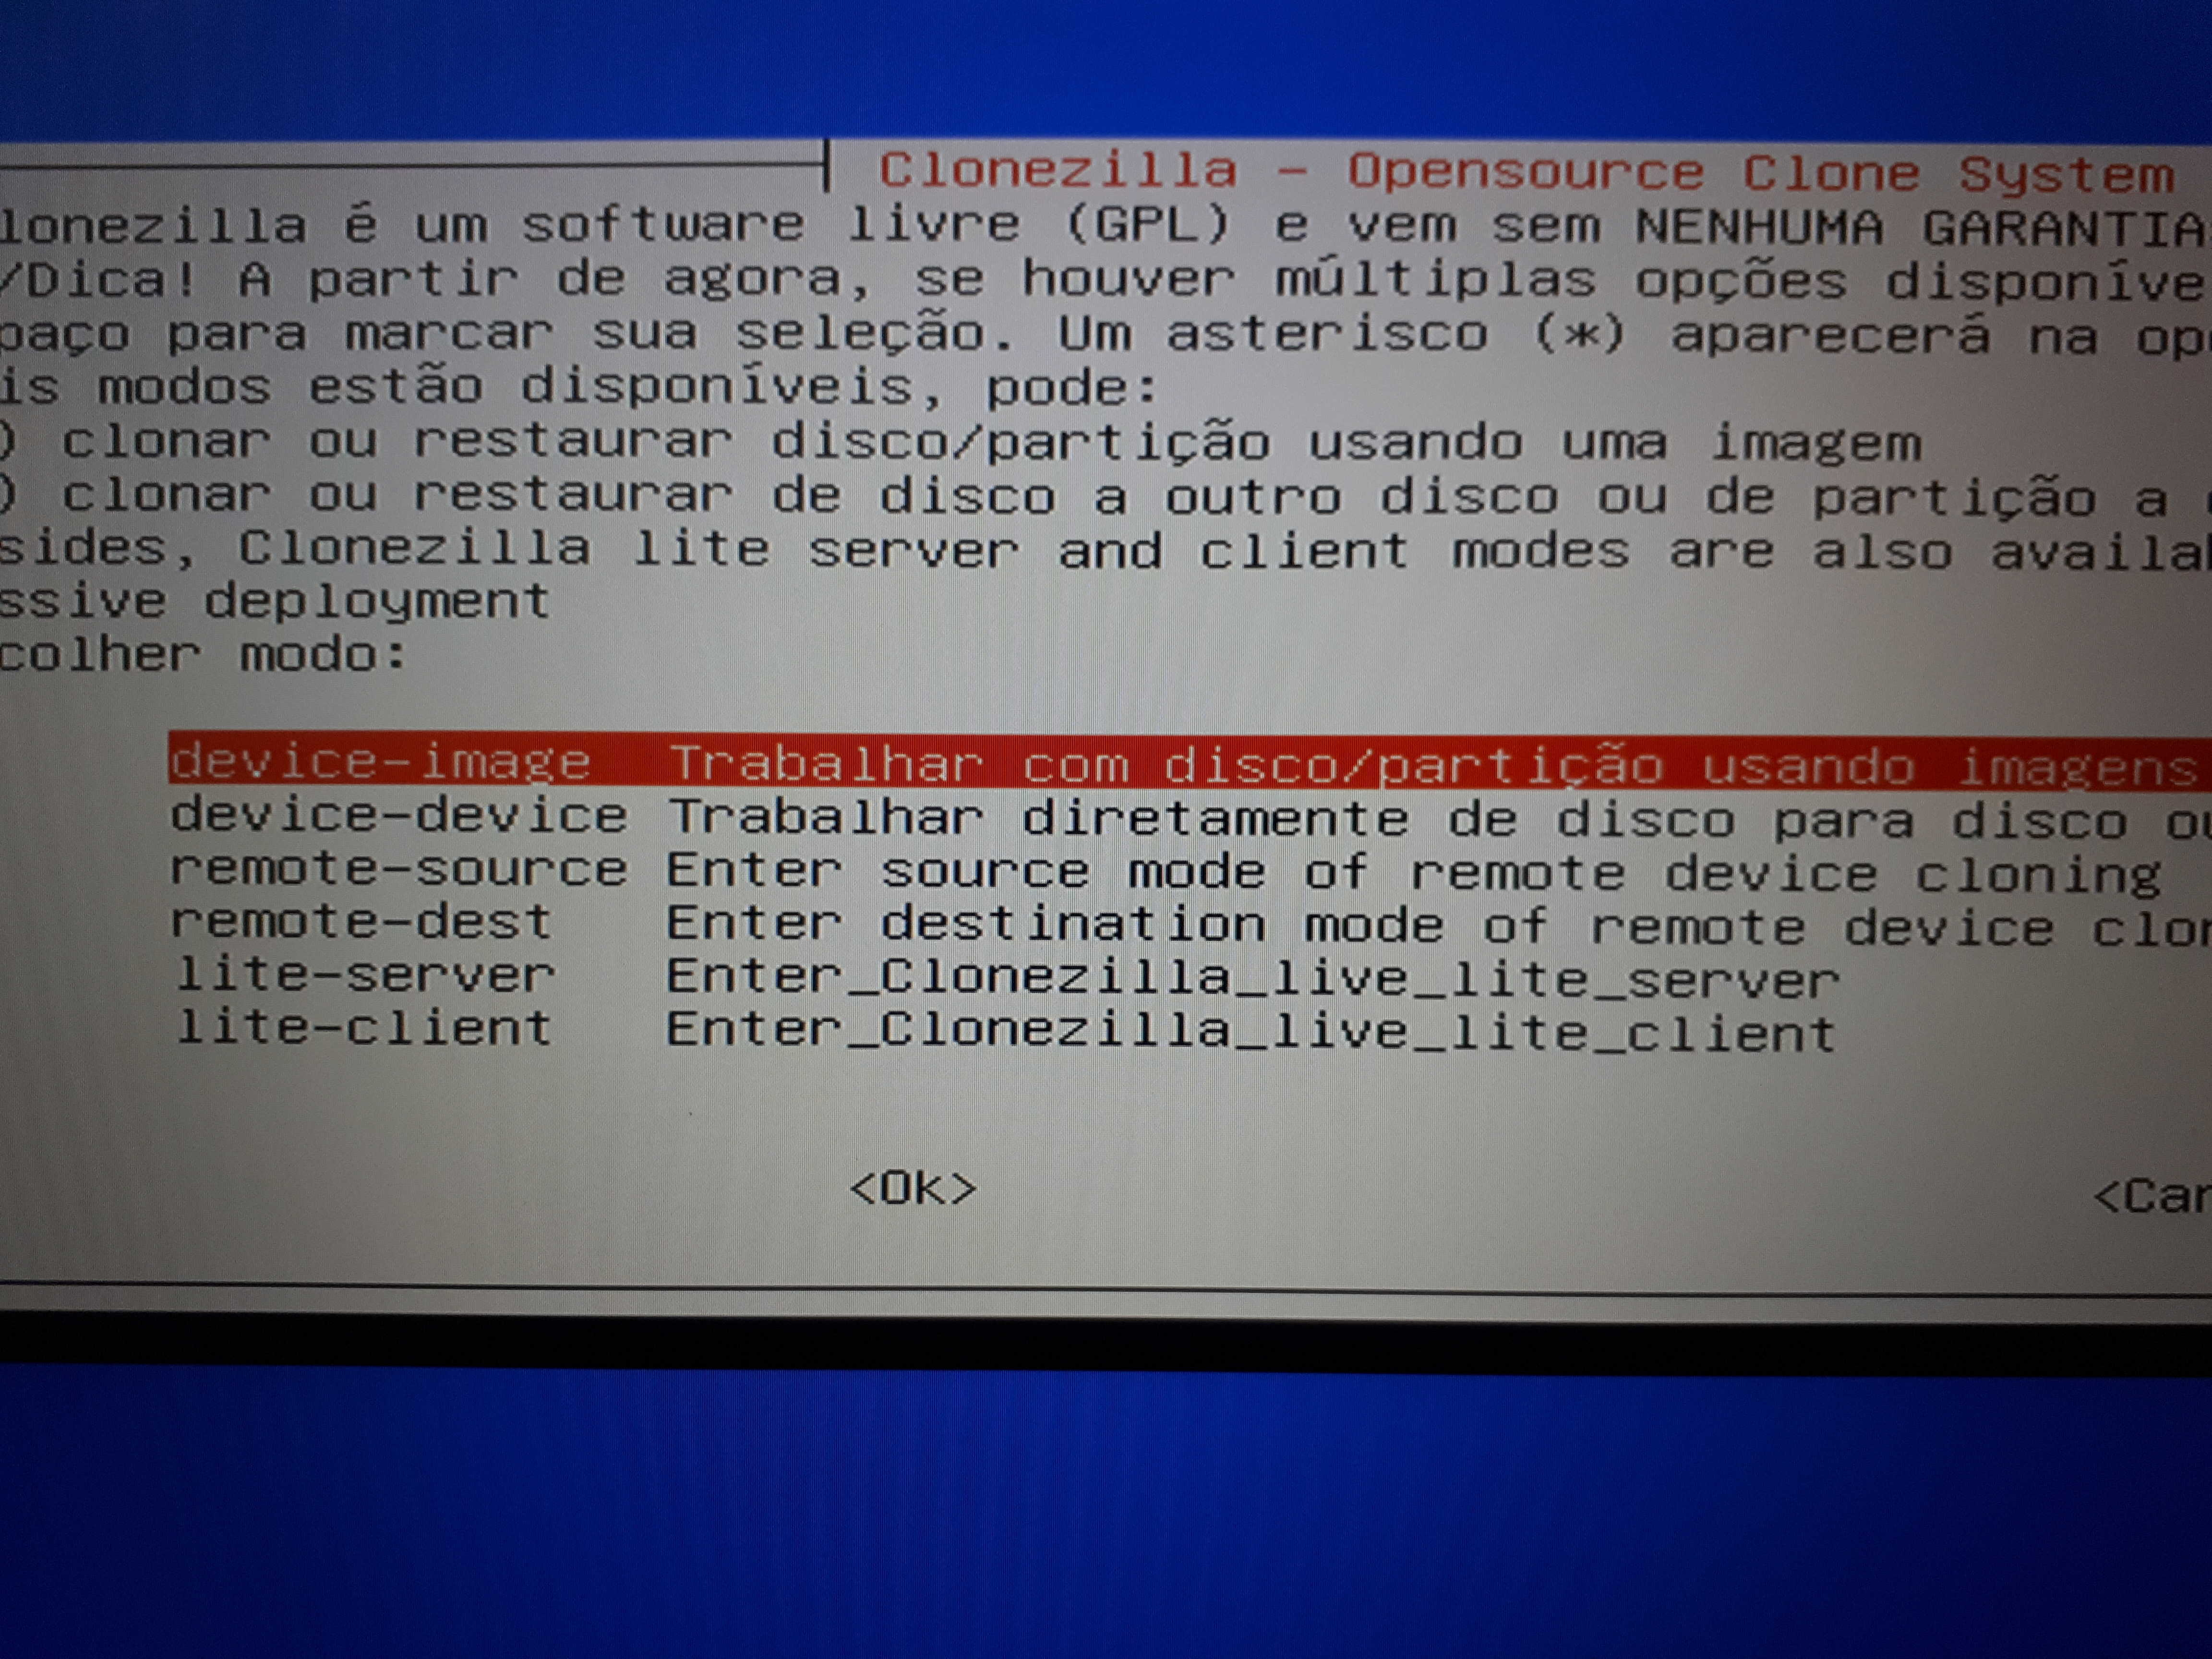
\includegraphics[width=1\linewidth]{images/backup/bkp6.jpg}
        \caption{Partições no Linux Programa GParted}
    \end{figure}
\end{frame}

\begin{frame}[plain,c]
   \frametitle{\insertsection}
    \framesubtitle{Localizar partição de DESTINO}
    \begin{figure}[!h]
        
        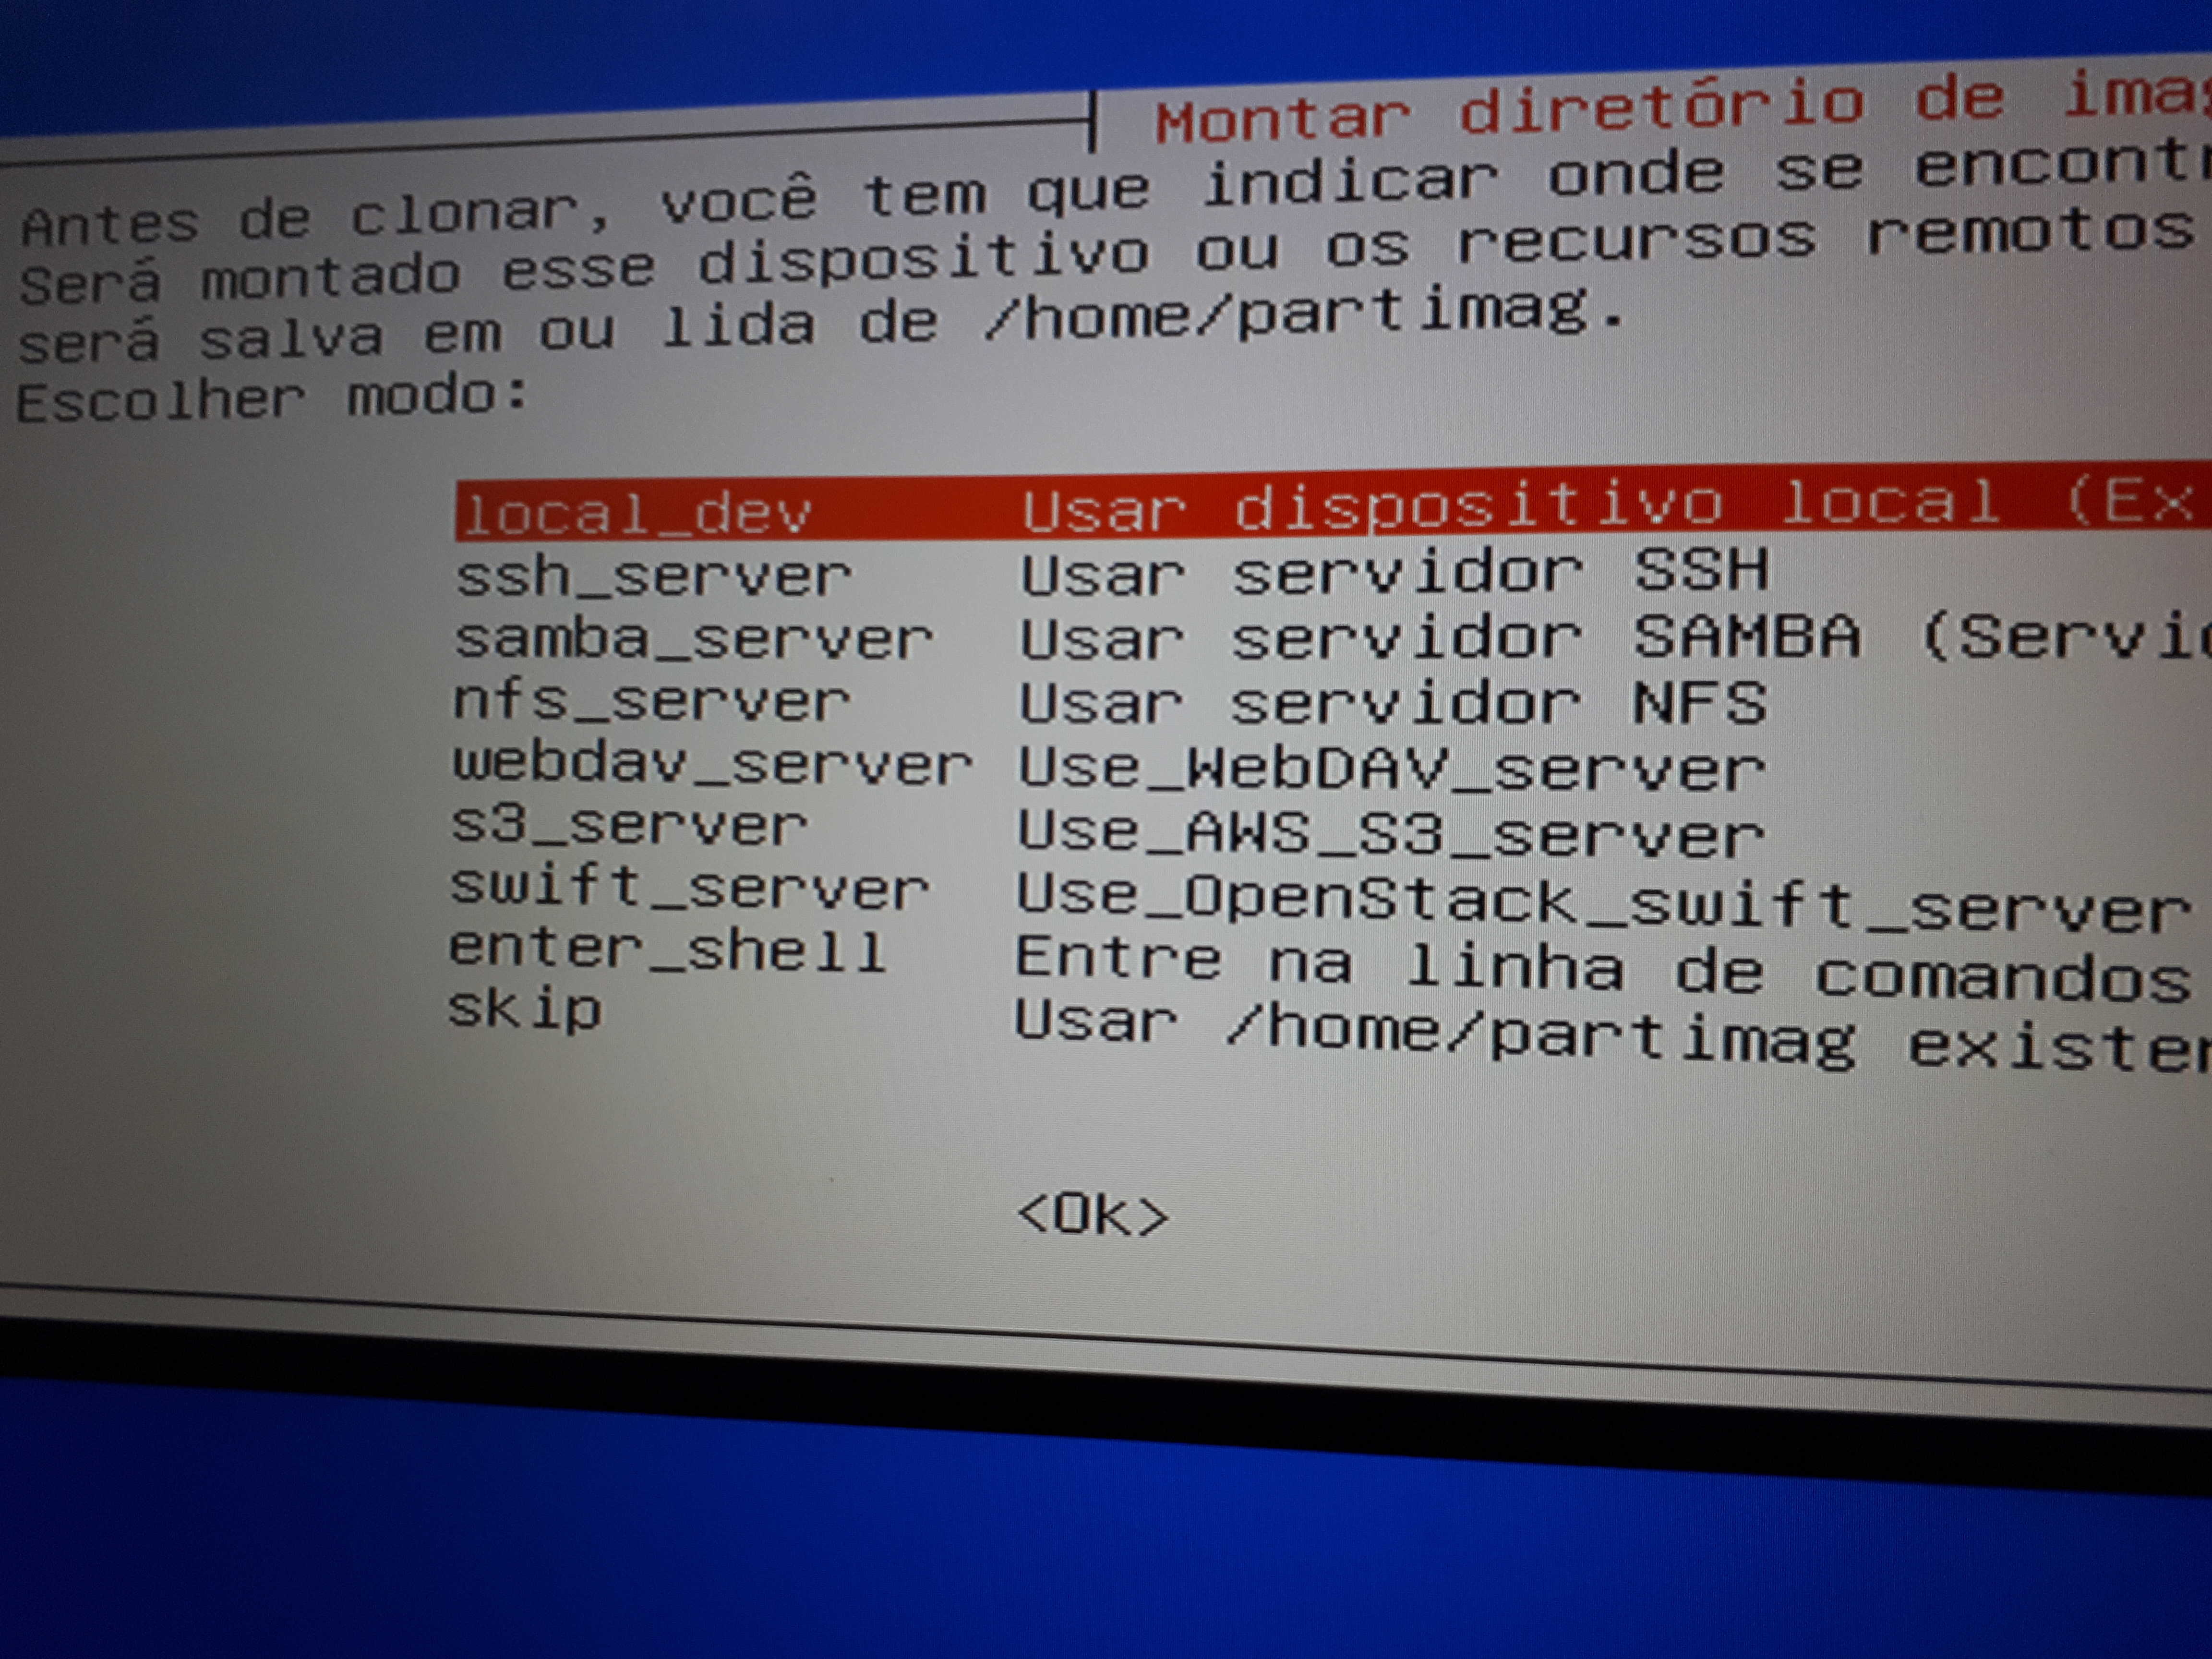
\includegraphics[width=1\linewidth]{images/backup/bkp7.jpg}
        \caption{Partições no Linux Programa GParted}
    \end{figure}
\end{frame}

\begin{frame}[plain,c]
   \frametitle{\insertsection}
    \framesubtitle{Para inserir HD Externo}
    \begin{figure}[!h]
        
        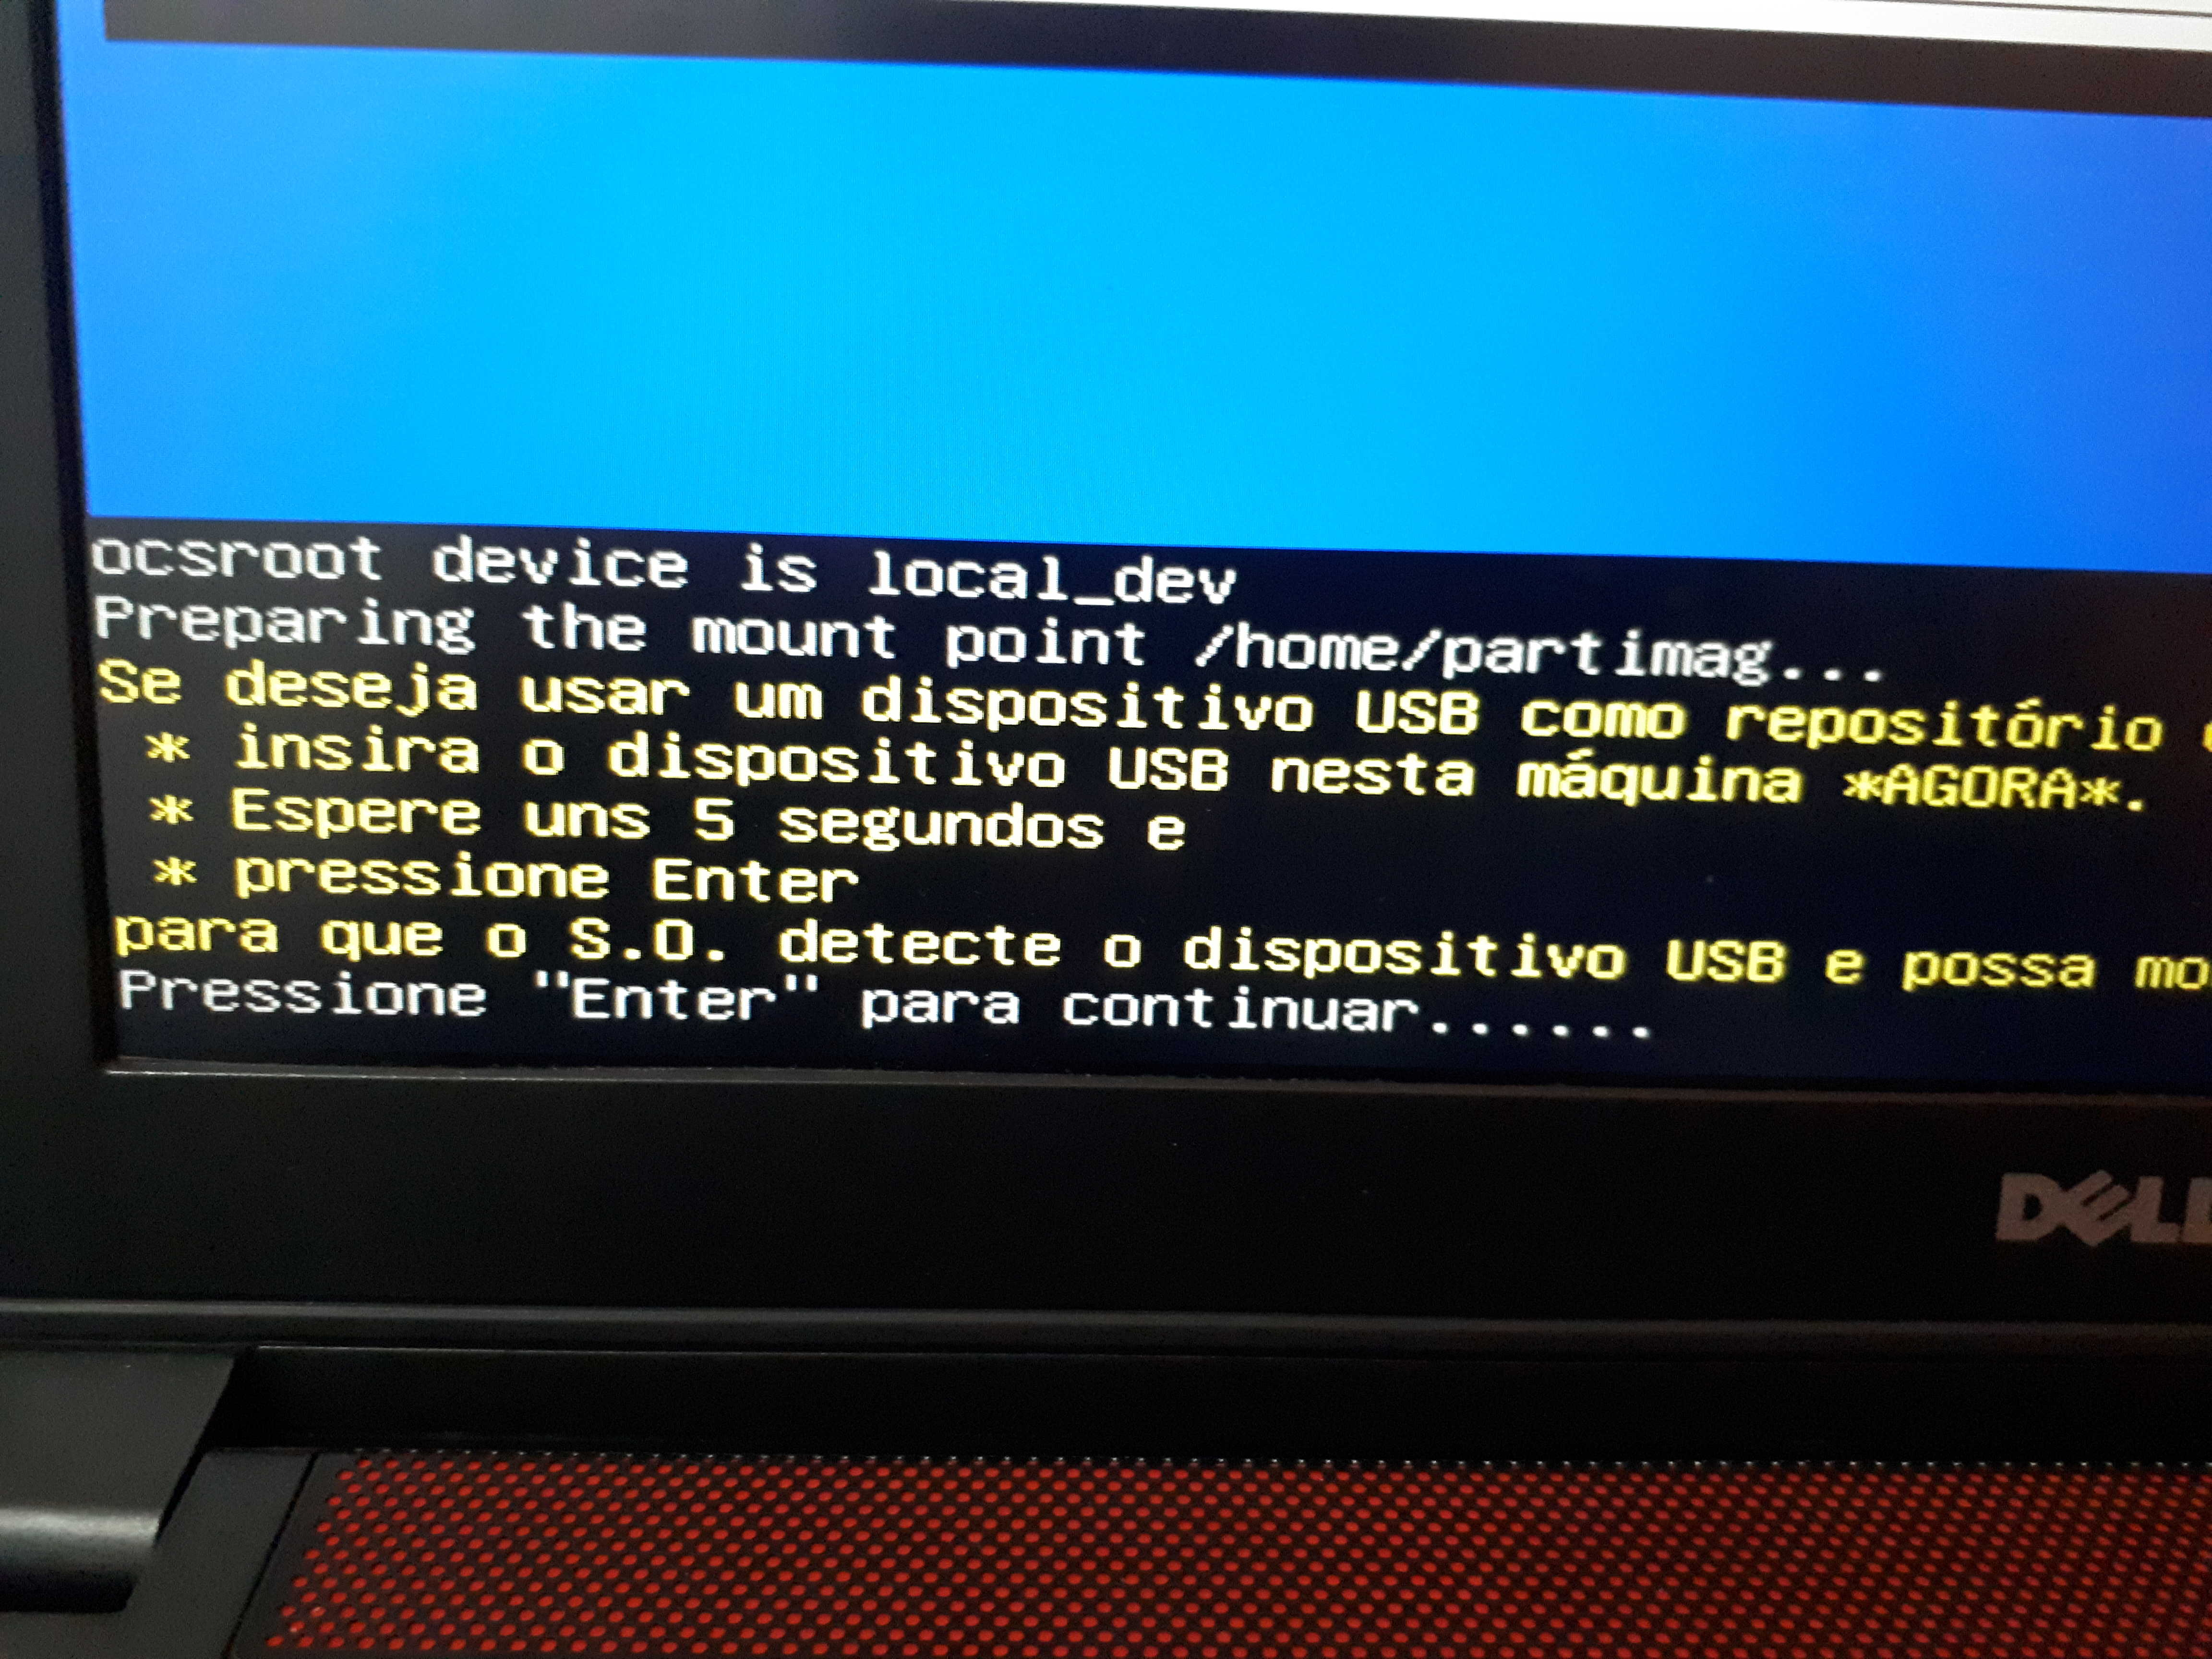
\includegraphics[width=1\linewidth]{images/backup/bkp8.jpg}
        \caption{Partições no Linux Programa GParted}
    \end{figure}
\end{frame}

\begin{frame}[plain,c]
   \frametitle{\insertsection}
    \framesubtitle{Todas os HDs disponíveis}
    \begin{figure}[!h]
        
        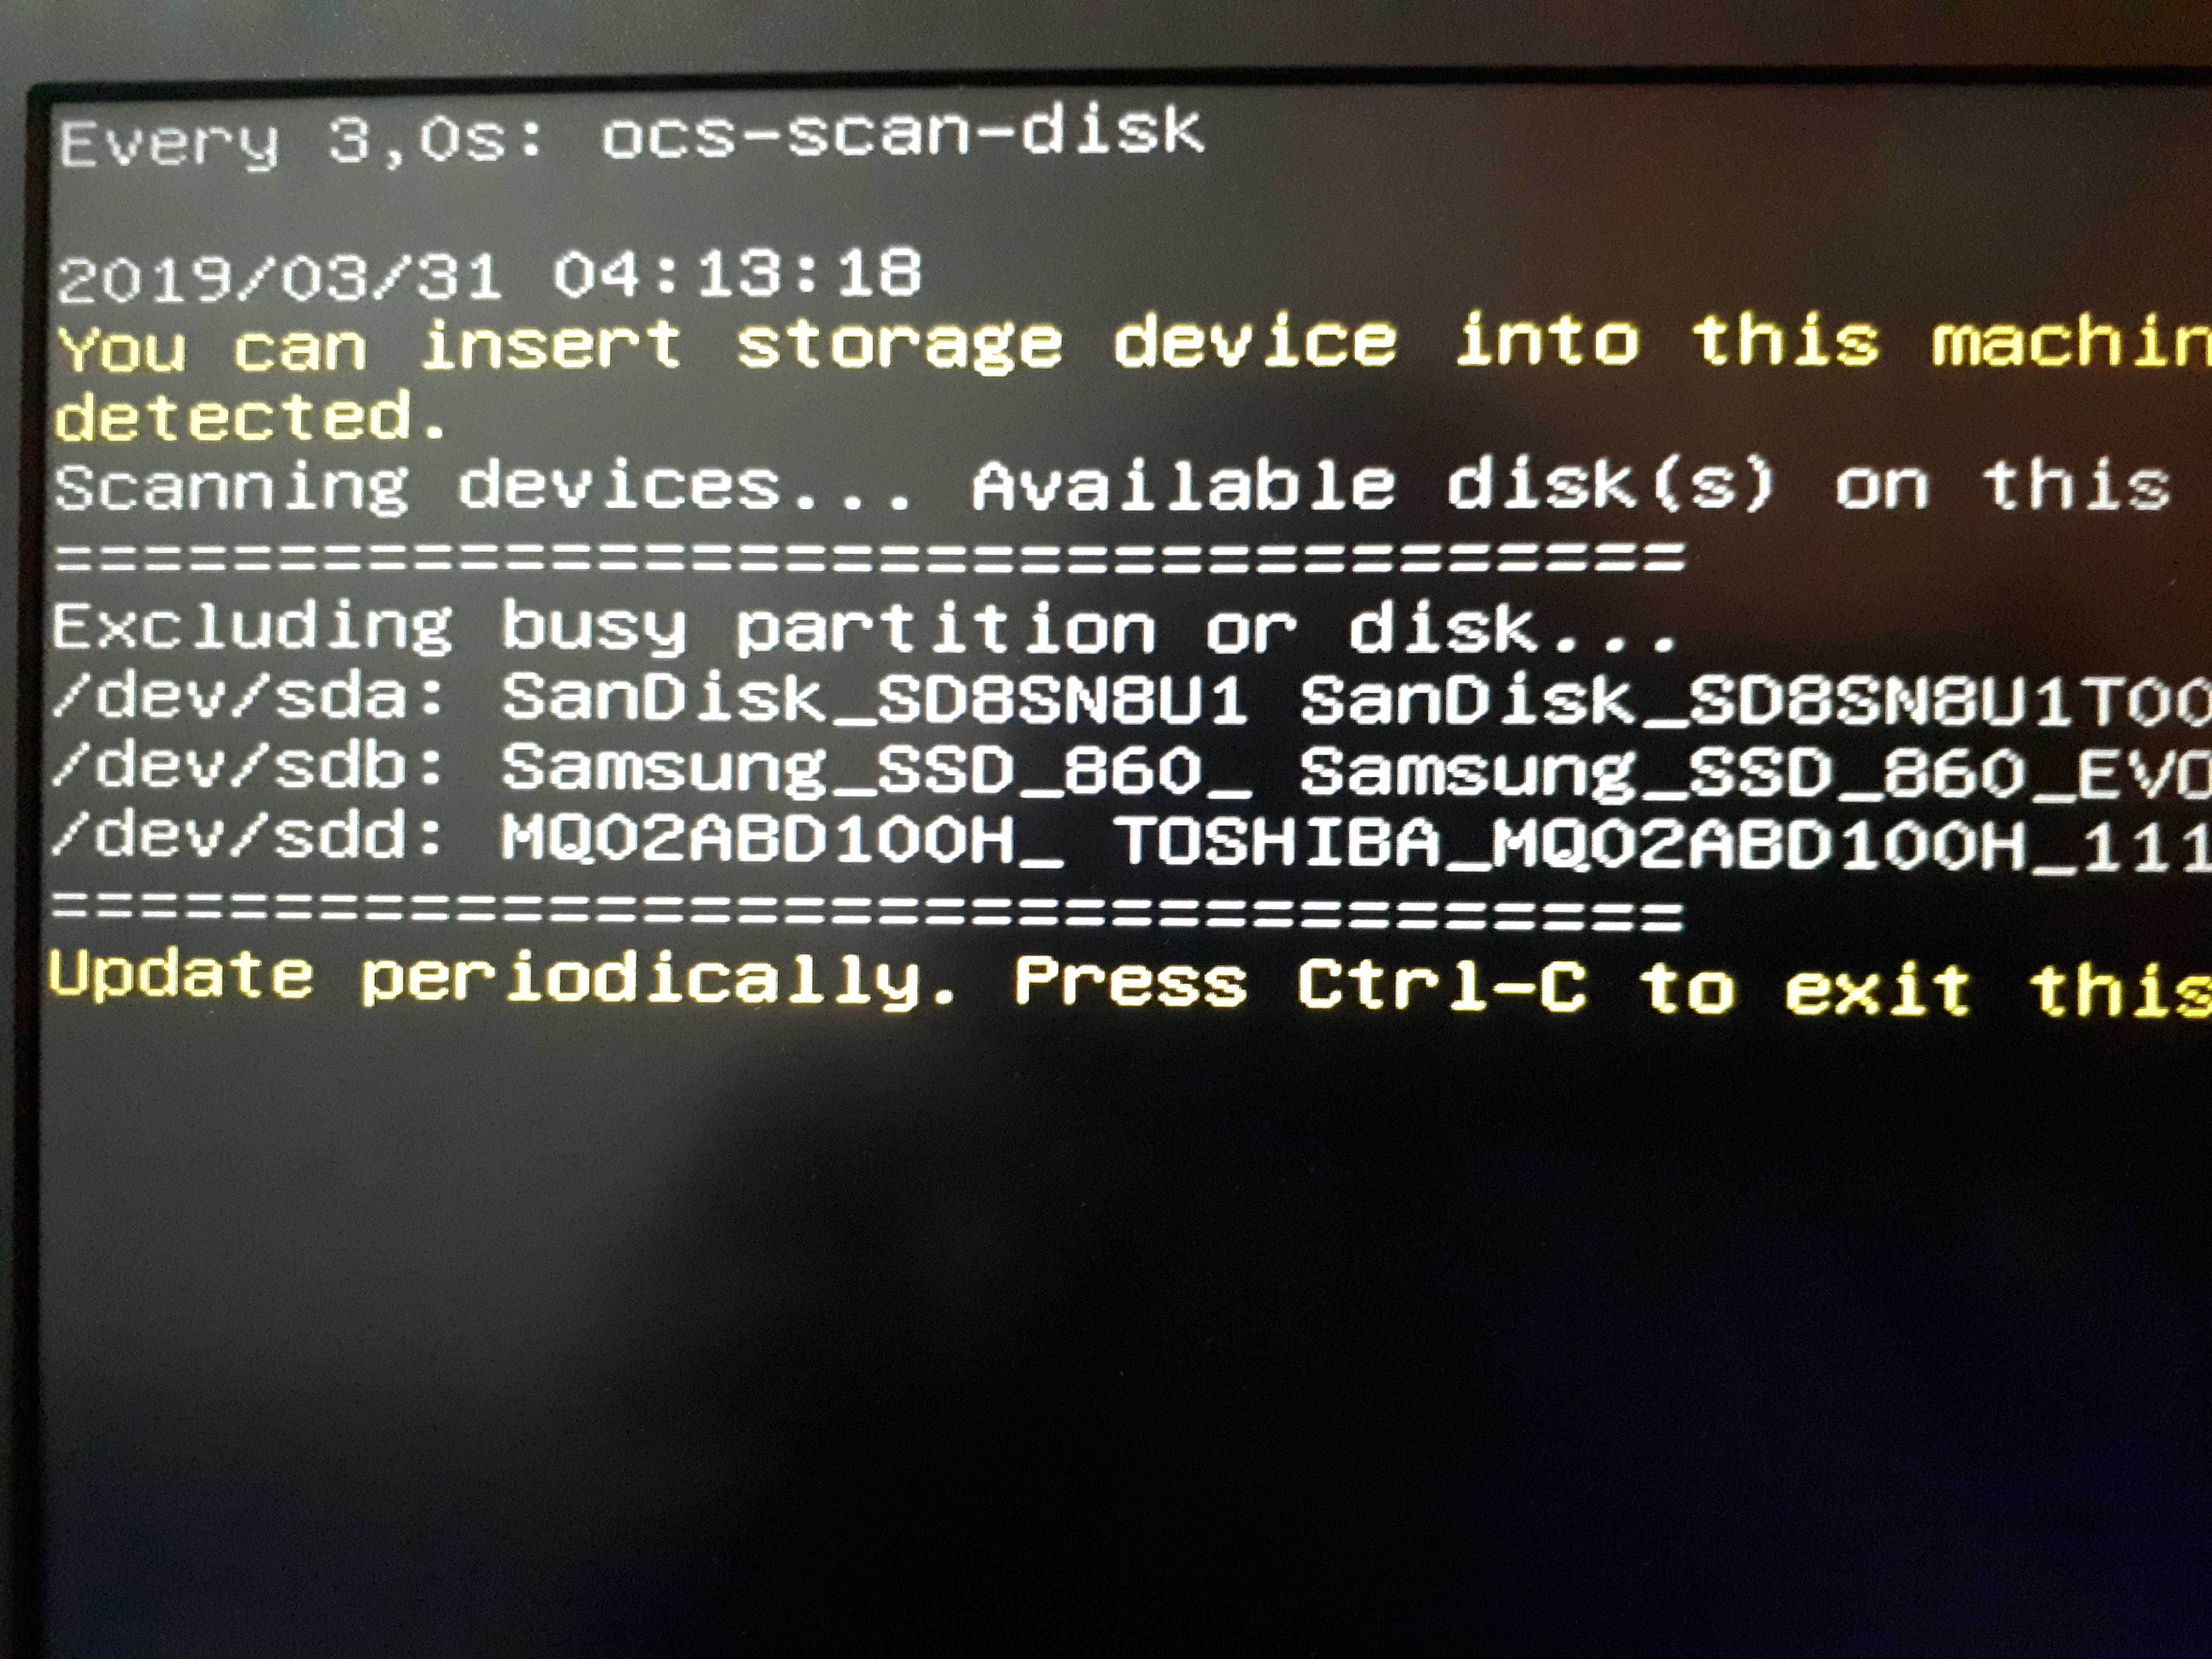
\includegraphics[width=1\linewidth]{images/backup/bkp9.jpg}
        \caption{Partições no Linux Programa GParted}
    \end{figure}
\end{frame}

\begin{frame}[plain,c]
   \frametitle{\insertsection}
    \framesubtitle{Escolhendo HD de DESTINO}
    \begin{figure}[!h]
        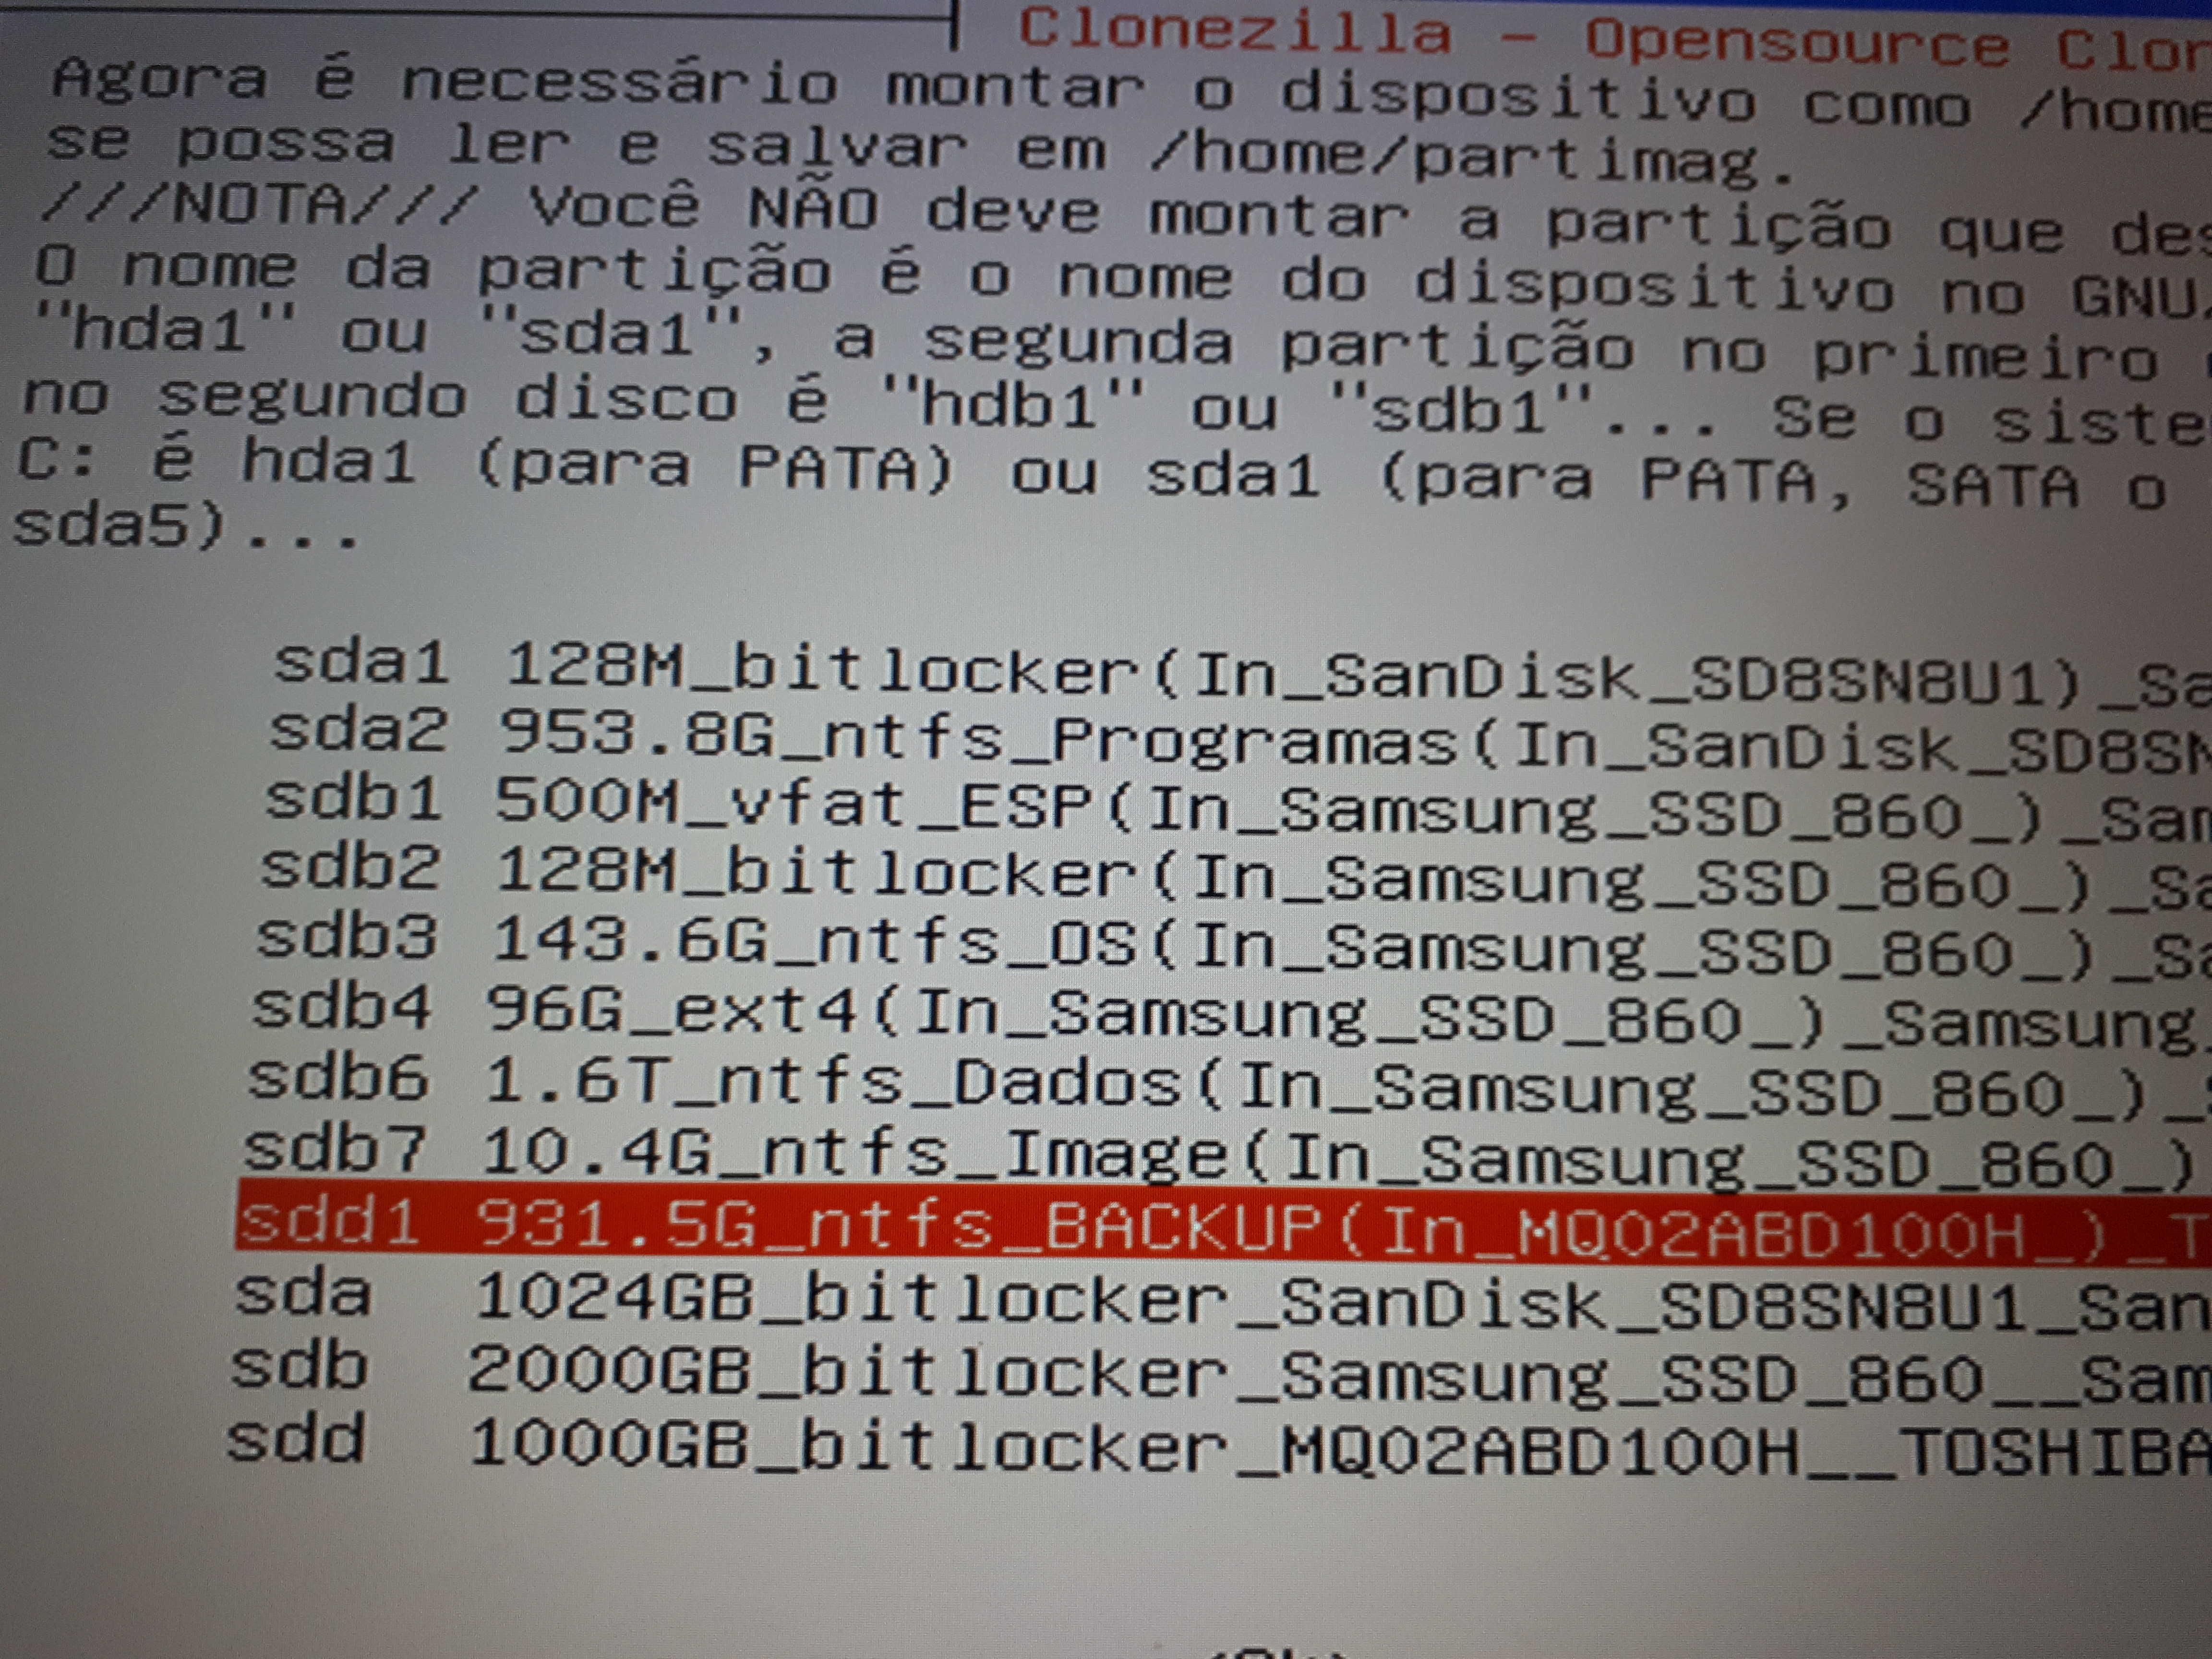
\includegraphics[width=1\linewidth]{images/backup/bkp10.jpg}
        \caption{Partições no Linux Programa GParted}
    \end{figure}
\end{frame}

\begin{frame}[plain,c]
   \frametitle{\insertsection}
    \framesubtitle{Escolhendo Diretório no HD de DESTINO}
    \begin{figure}[!h]
        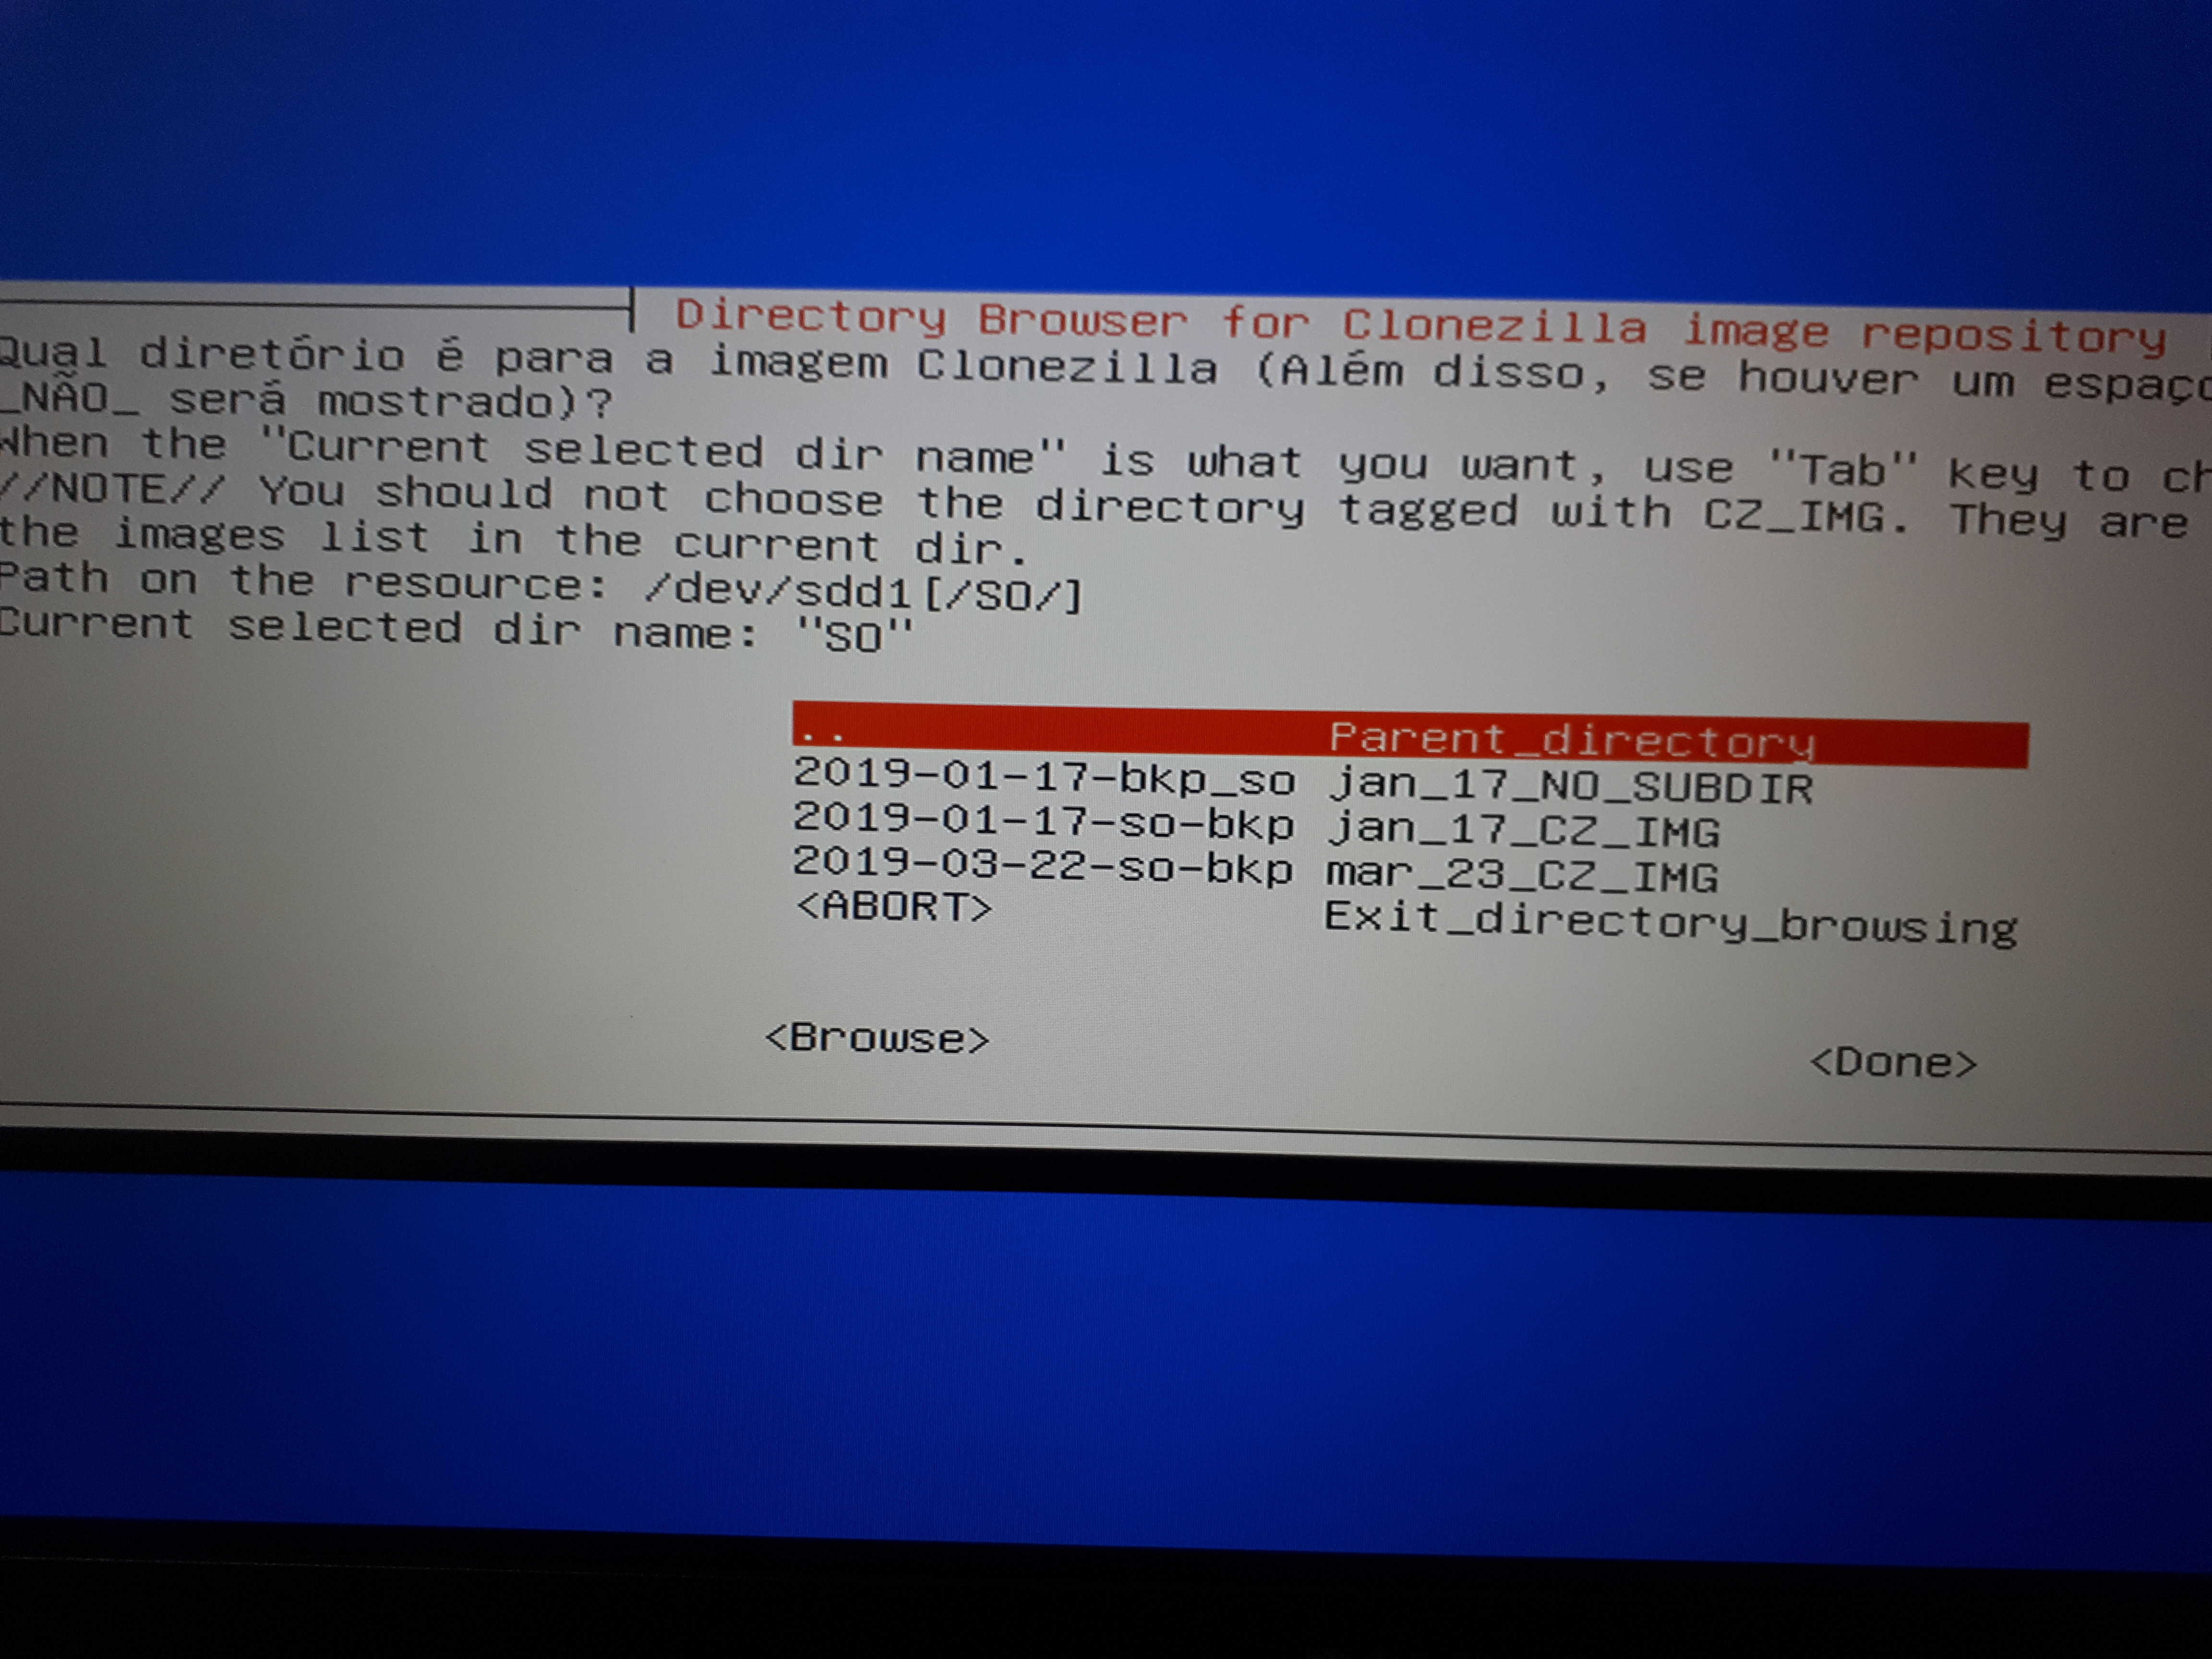
\includegraphics[width=1\linewidth]{images/backup/bkp11.jpg}
        \caption{Partições no Linux Programa GParted}
    \end{figure}
\end{frame}

\begin{frame}[plain,c]
   \frametitle{\insertsection}
    \framesubtitle{Escolhendo Diretório no HD de DESTINO}
    \begin{figure}[!h]
        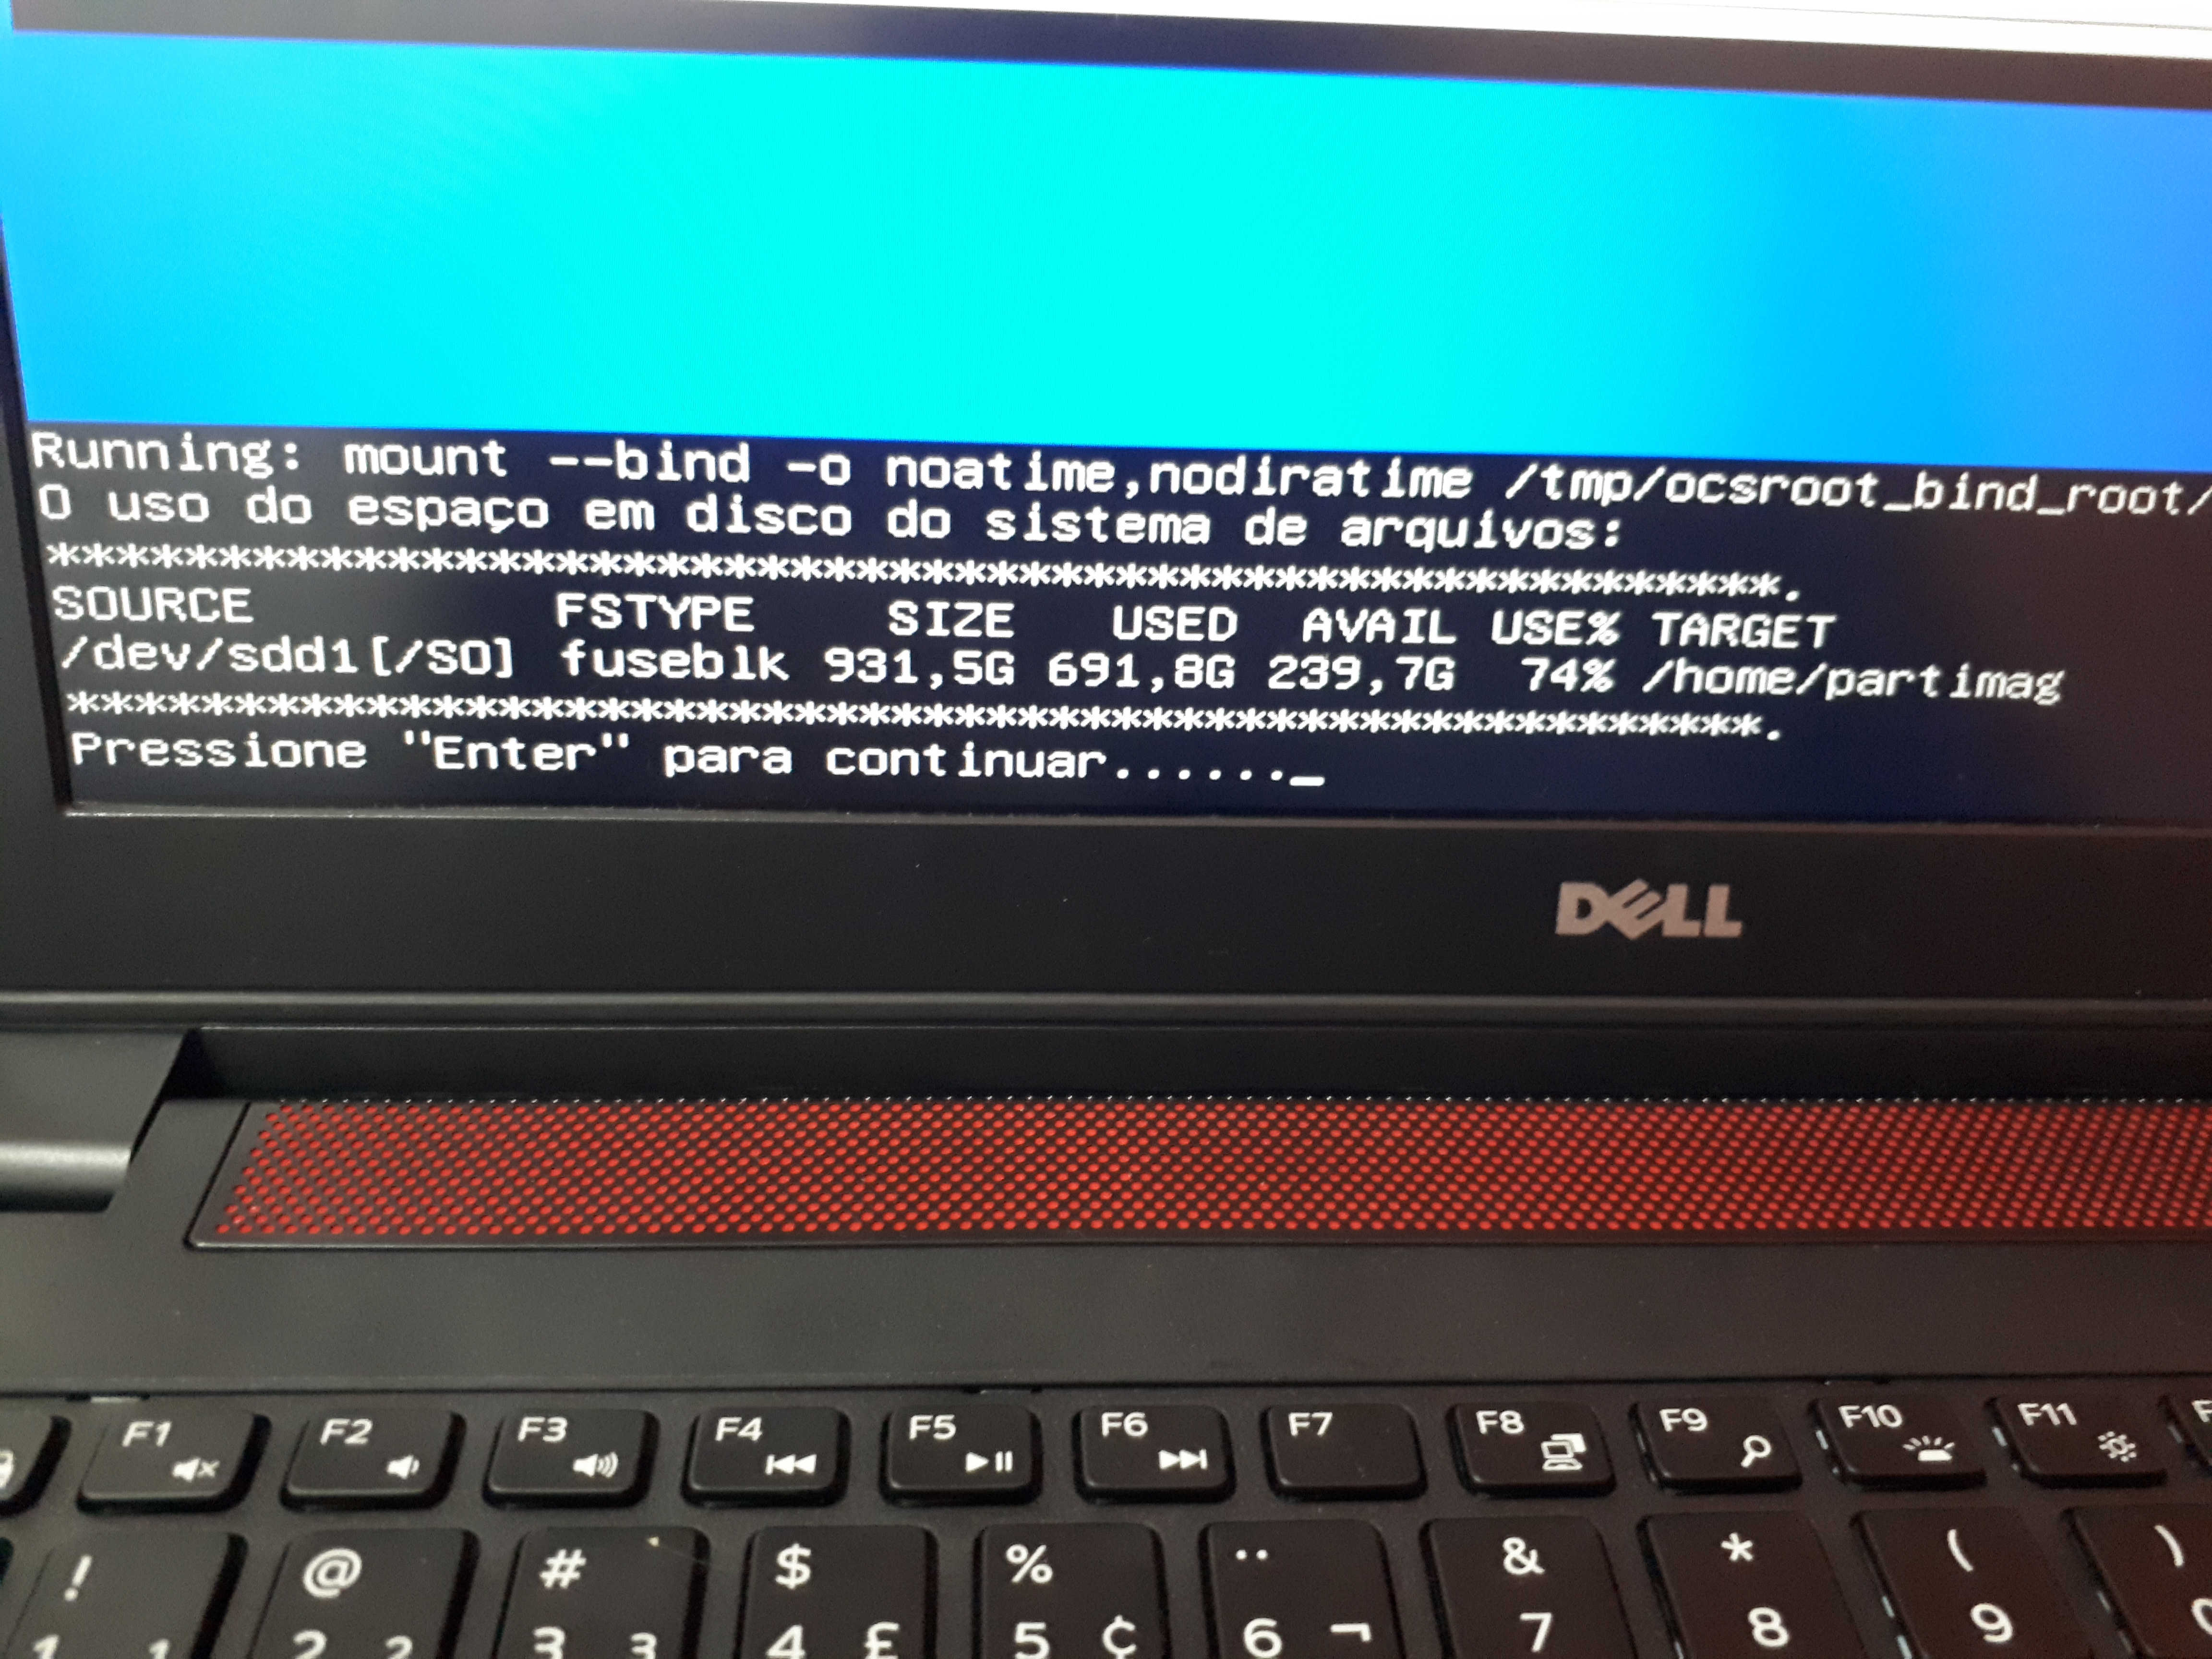
\includegraphics[width=1\linewidth]{images/backup/bkp12.jpg}
        \caption{Partições no Linux Programa GParted}
    \end{figure}
\end{frame}


\begin{frame}[plain,c]
   \frametitle{\insertsection}
    \framesubtitle{Escolhendo Diretório no HD de DESTINO}
    \begin{figure}[!h]
        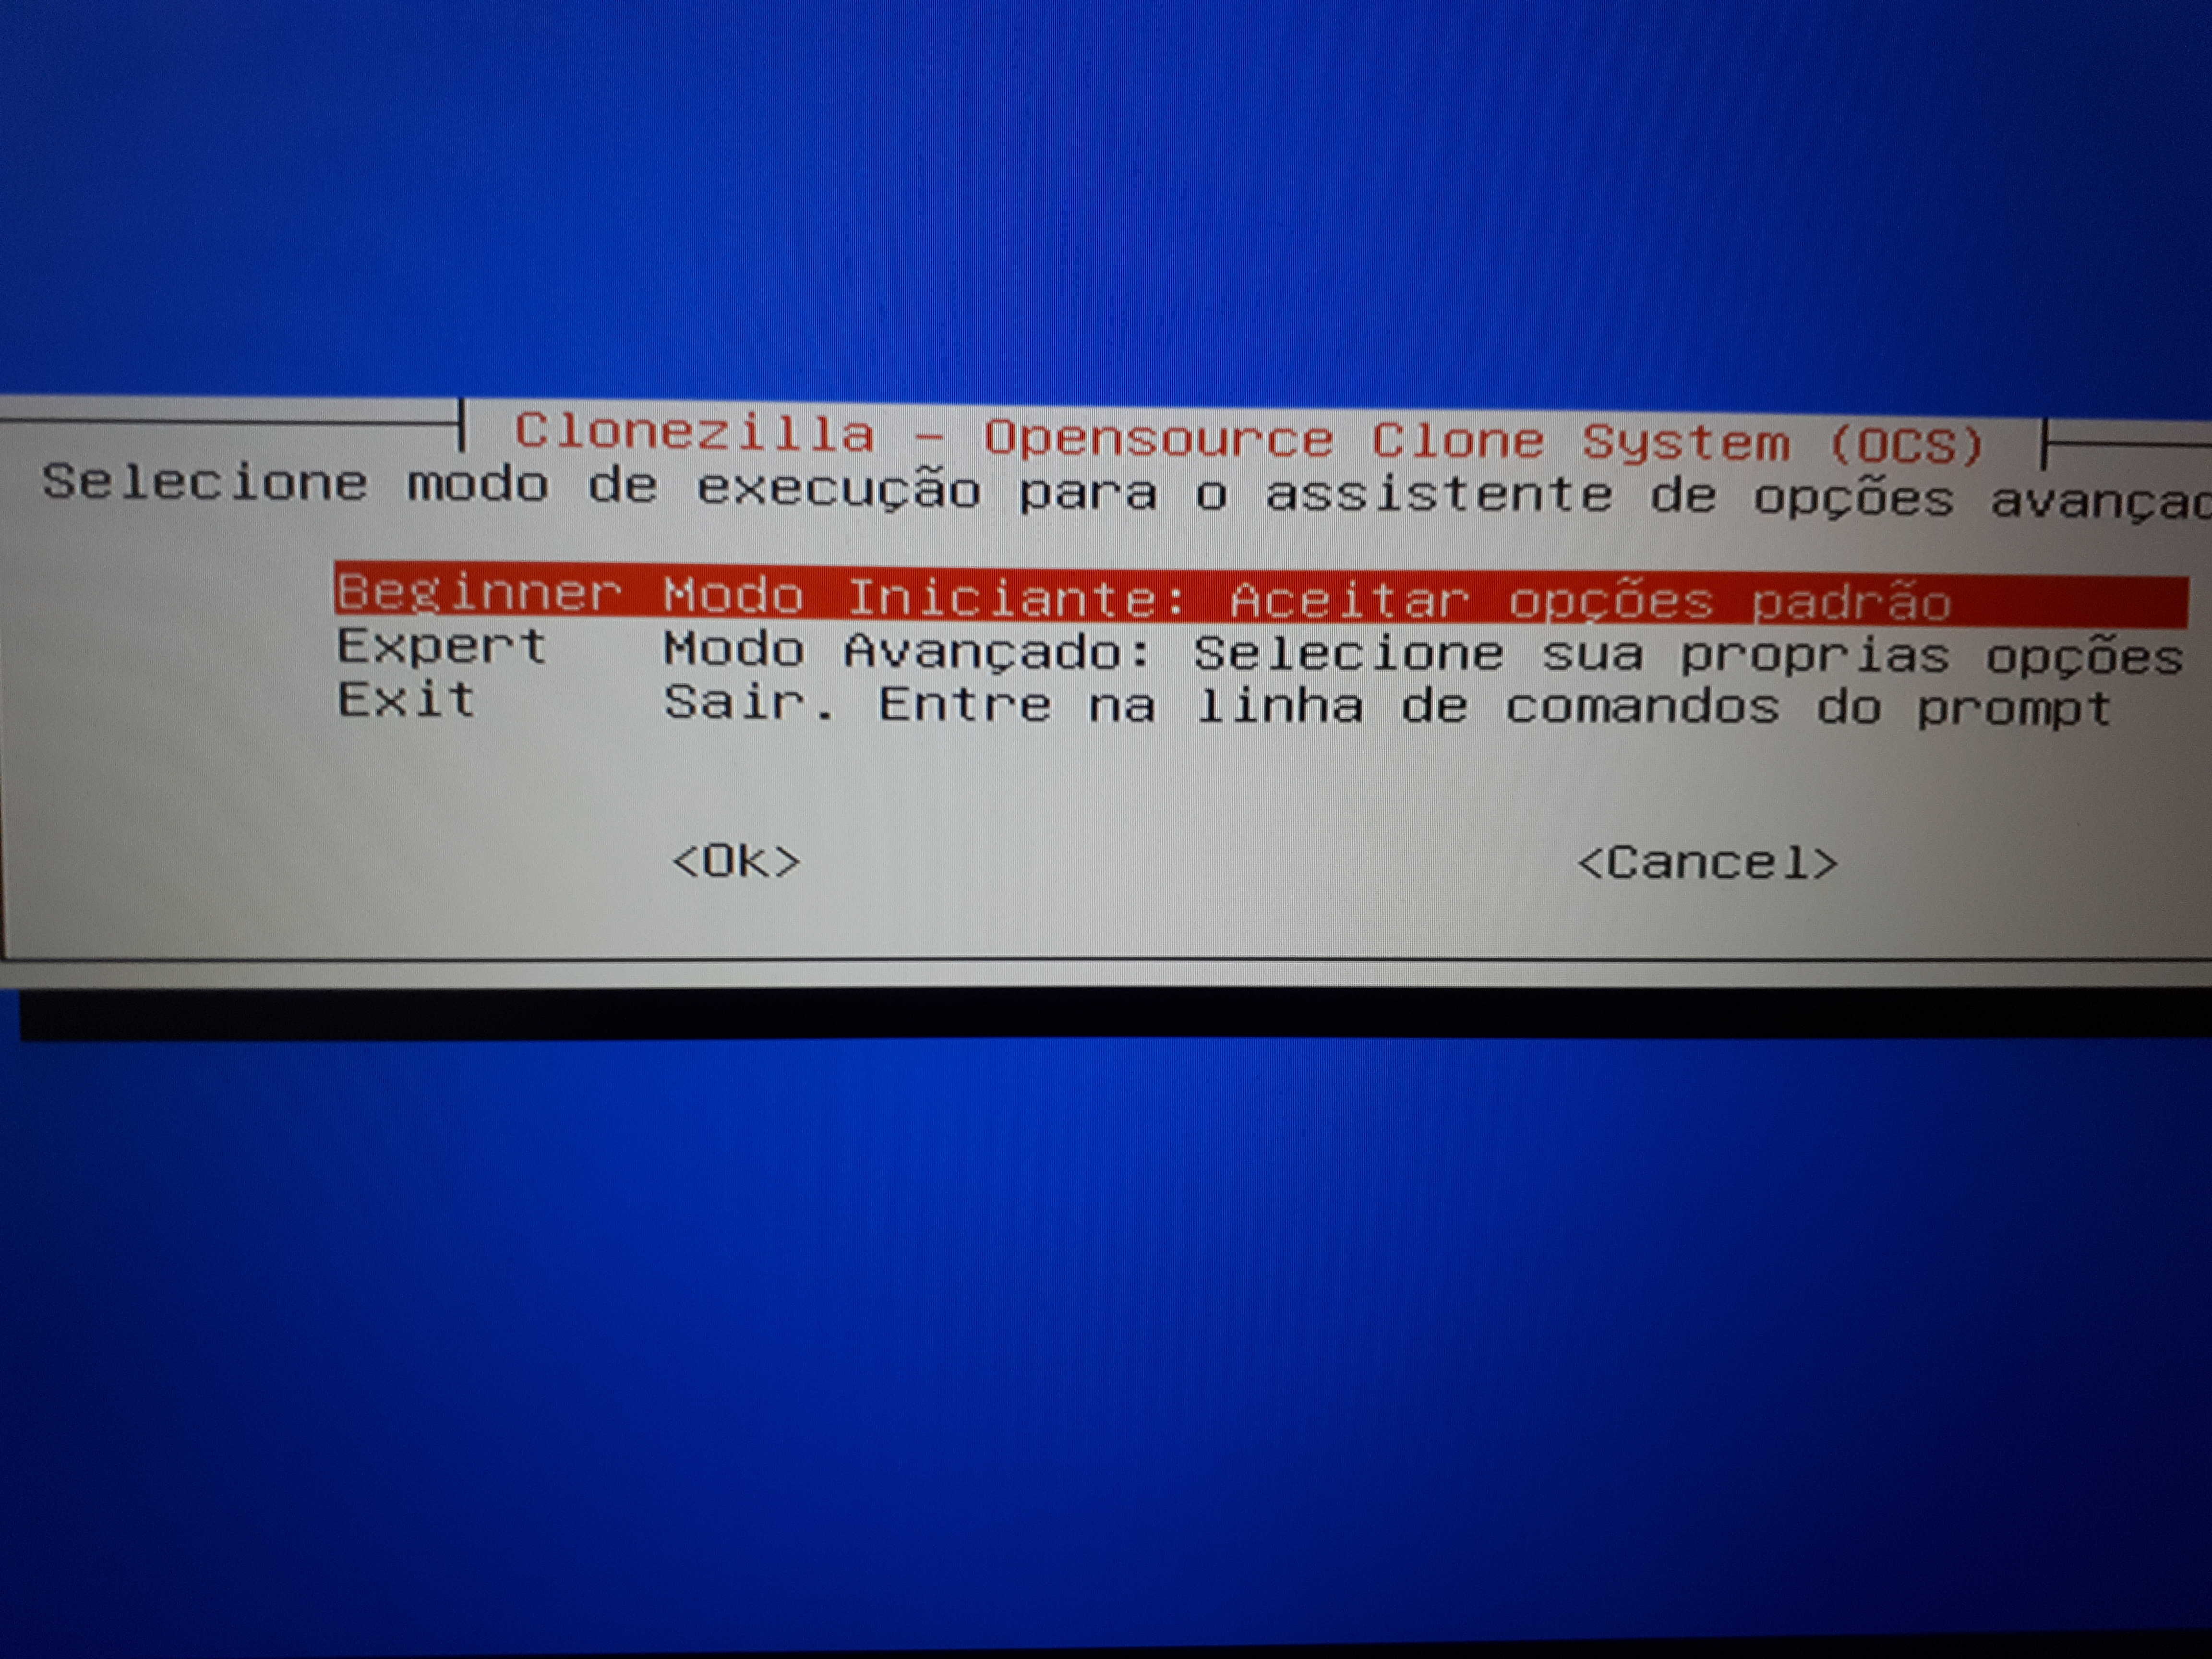
\includegraphics[width=1\linewidth]{images/backup/bkp13.jpg}
        \caption{Partições no Linux Programa GParted}
    \end{figure}
\end{frame}

\begin{frame}[plain,c]
   \frametitle{\insertsection}
    \framesubtitle{Escolher SAVEPARTS SALVAR PARTIÇÃO}
    \begin{figure}[!h]
        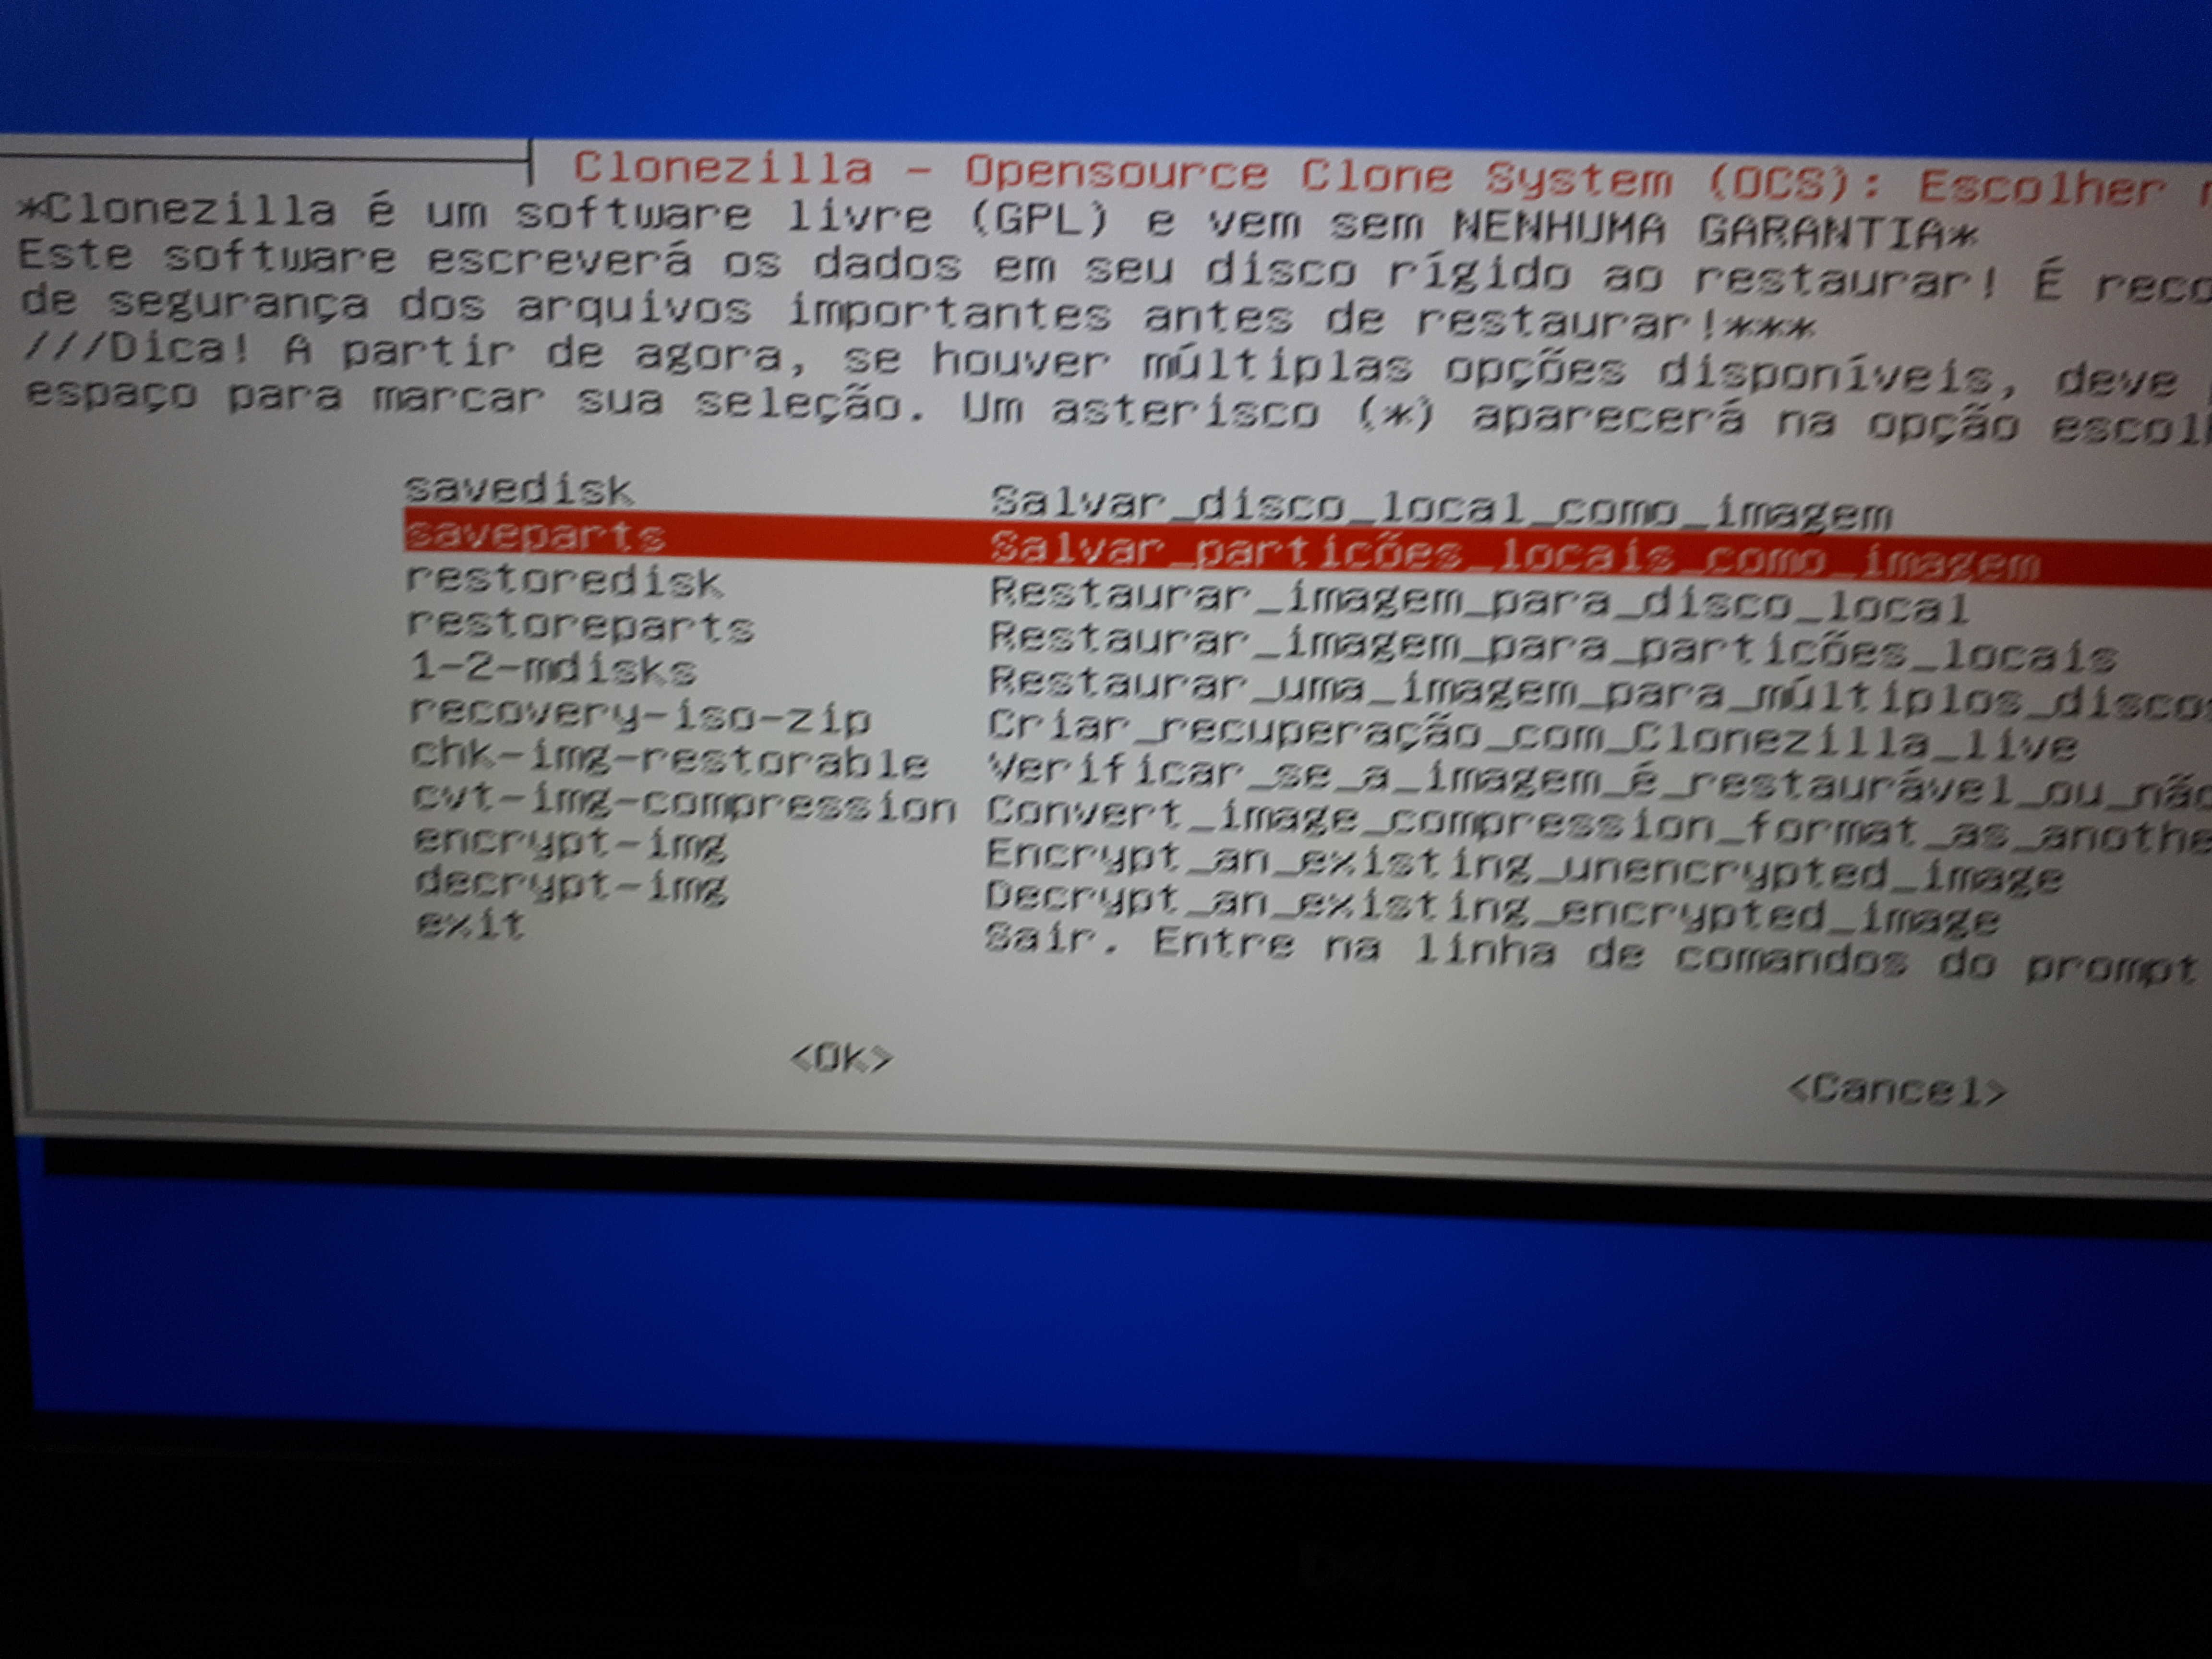
\includegraphics[width=1\linewidth]{images/backup/bkp14.jpg}
        \caption{Partições no Linux Programa GParted}
    \end{figure}
\end{frame}
\begin{frame}[plain,c]
   \frametitle{\insertsection}
    \framesubtitle{Escolher SAVEPARTS SALVAR PARTIÇÃO}
    \begin{figure}[!h]
        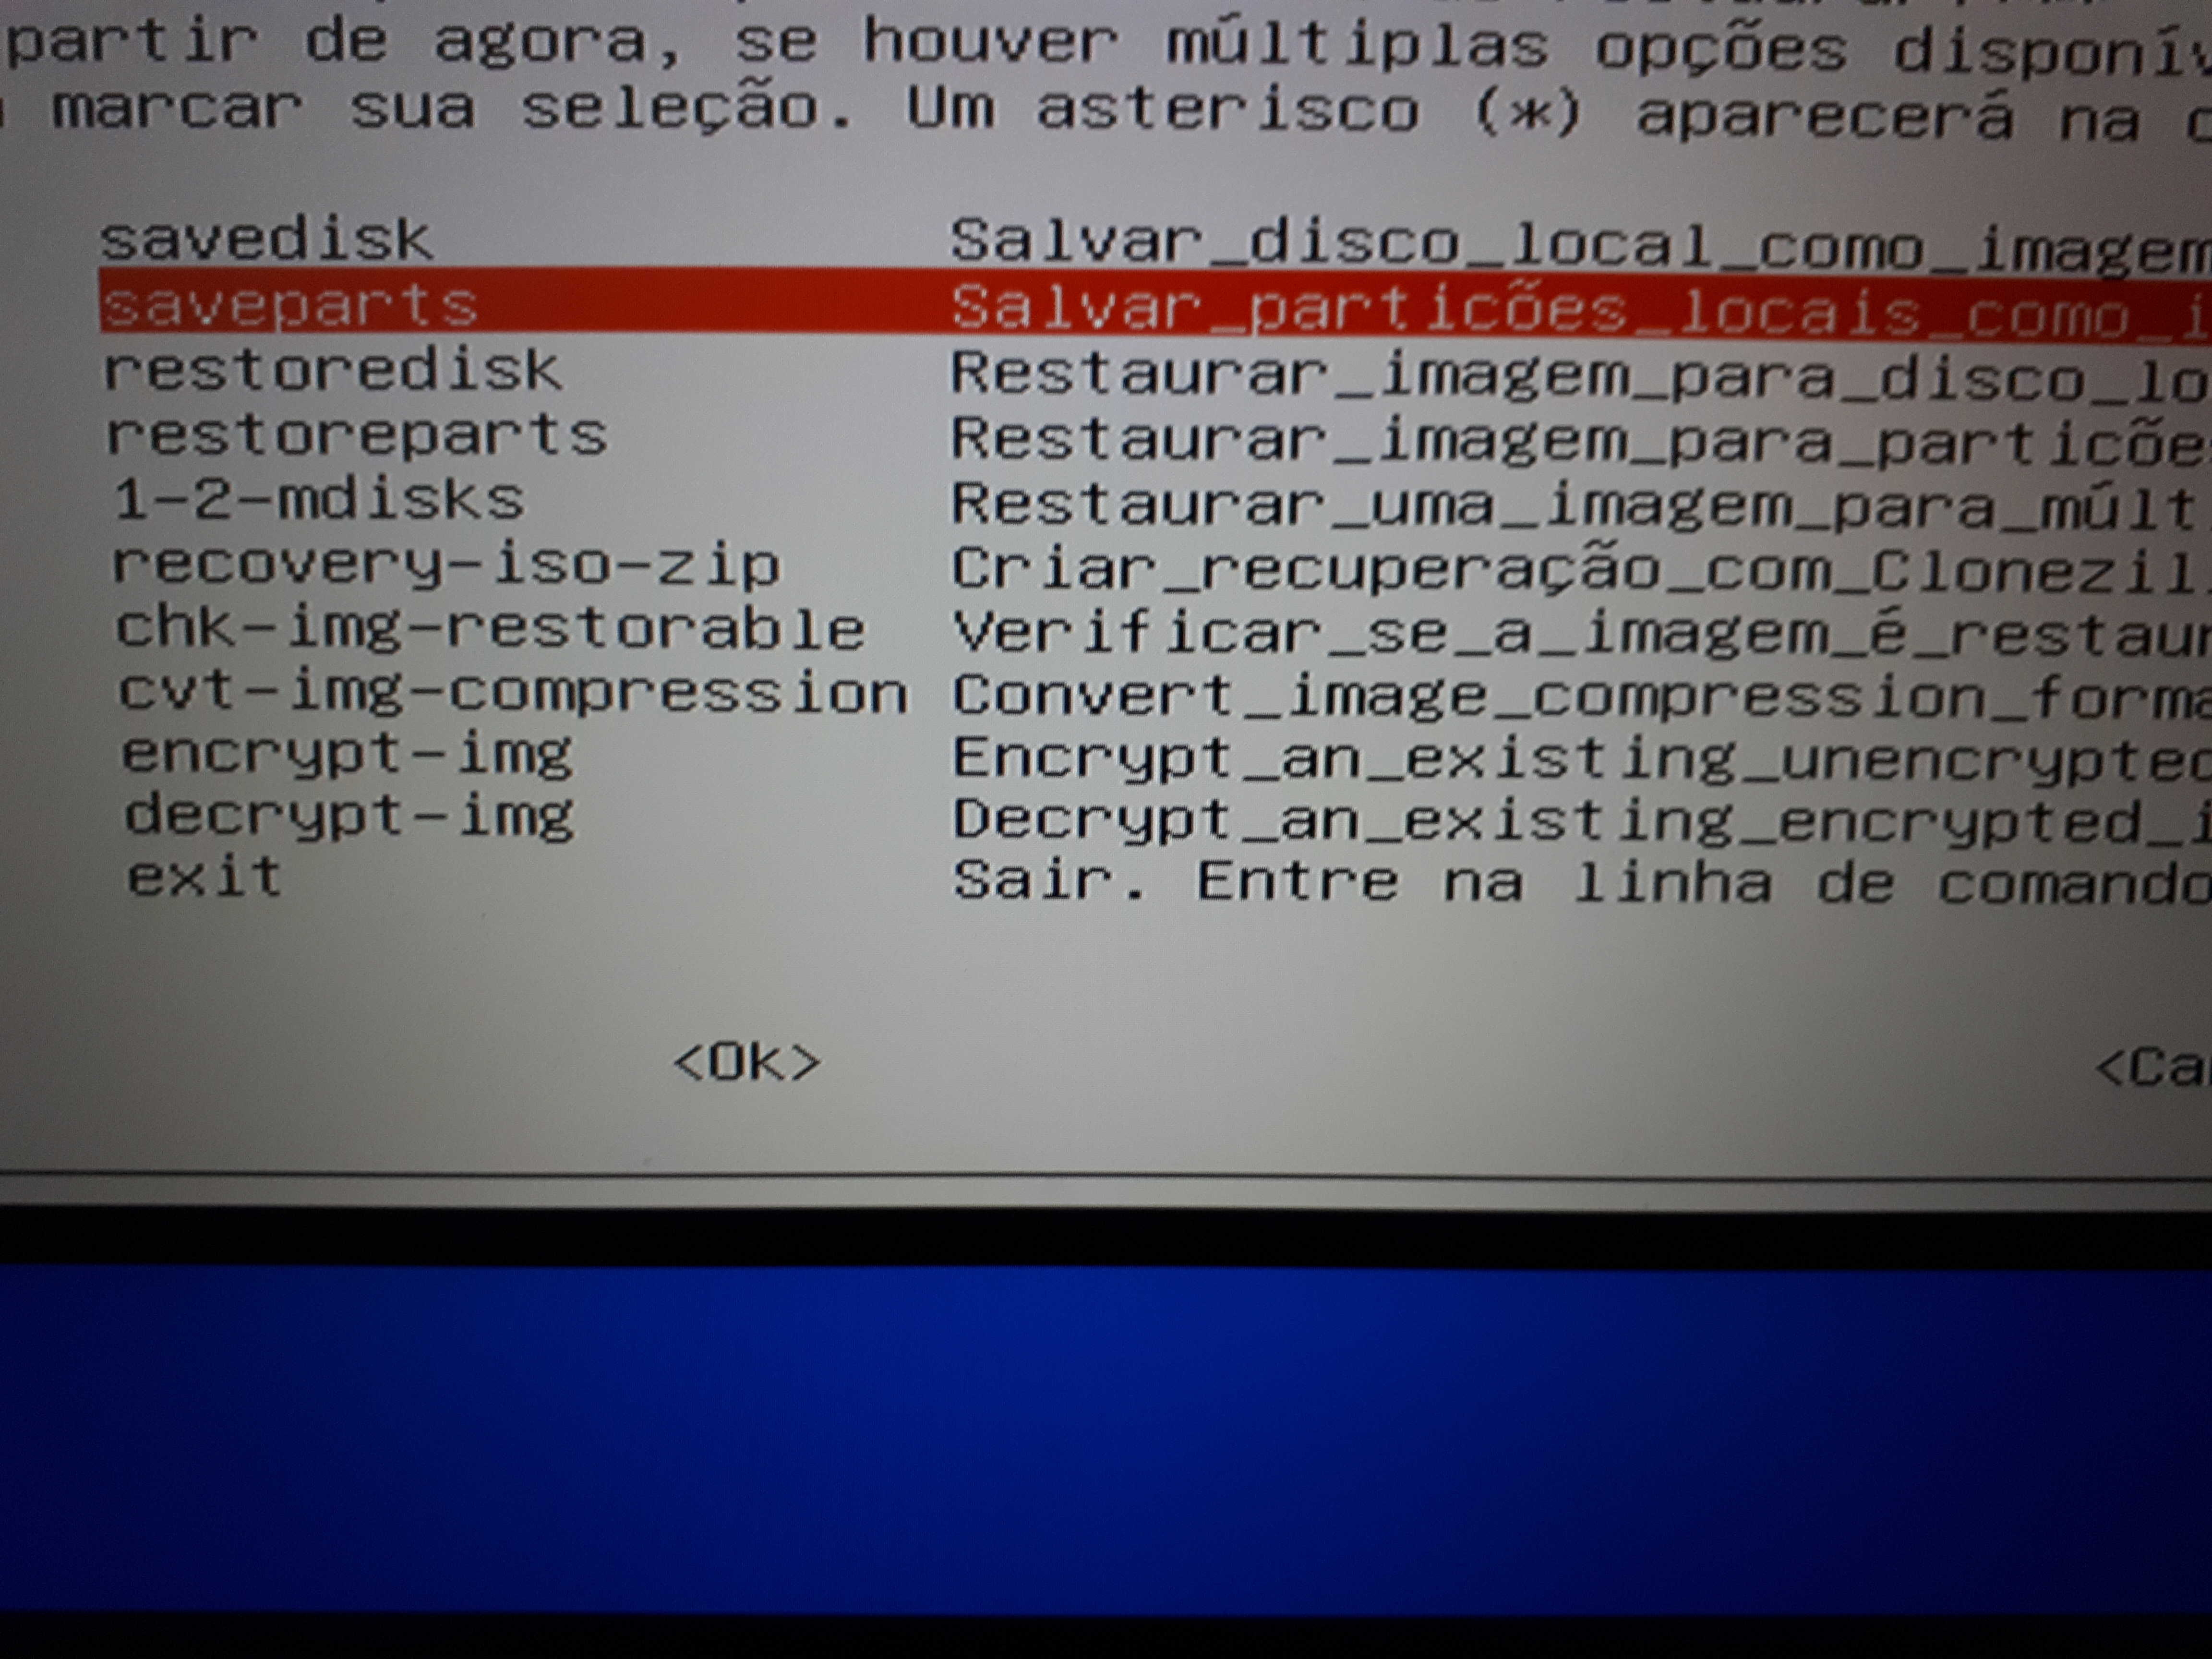
\includegraphics[width=1\linewidth]{images/backup/bkp15.jpg}
        \caption{Partições no Linux Programa GParted}
    \end{figure}
\end{frame}
\begin{frame}[plain,c]
   \frametitle{\insertsection}
    \framesubtitle{Nome do arquivo de IMAGEM}
    \begin{figure}[!h]
        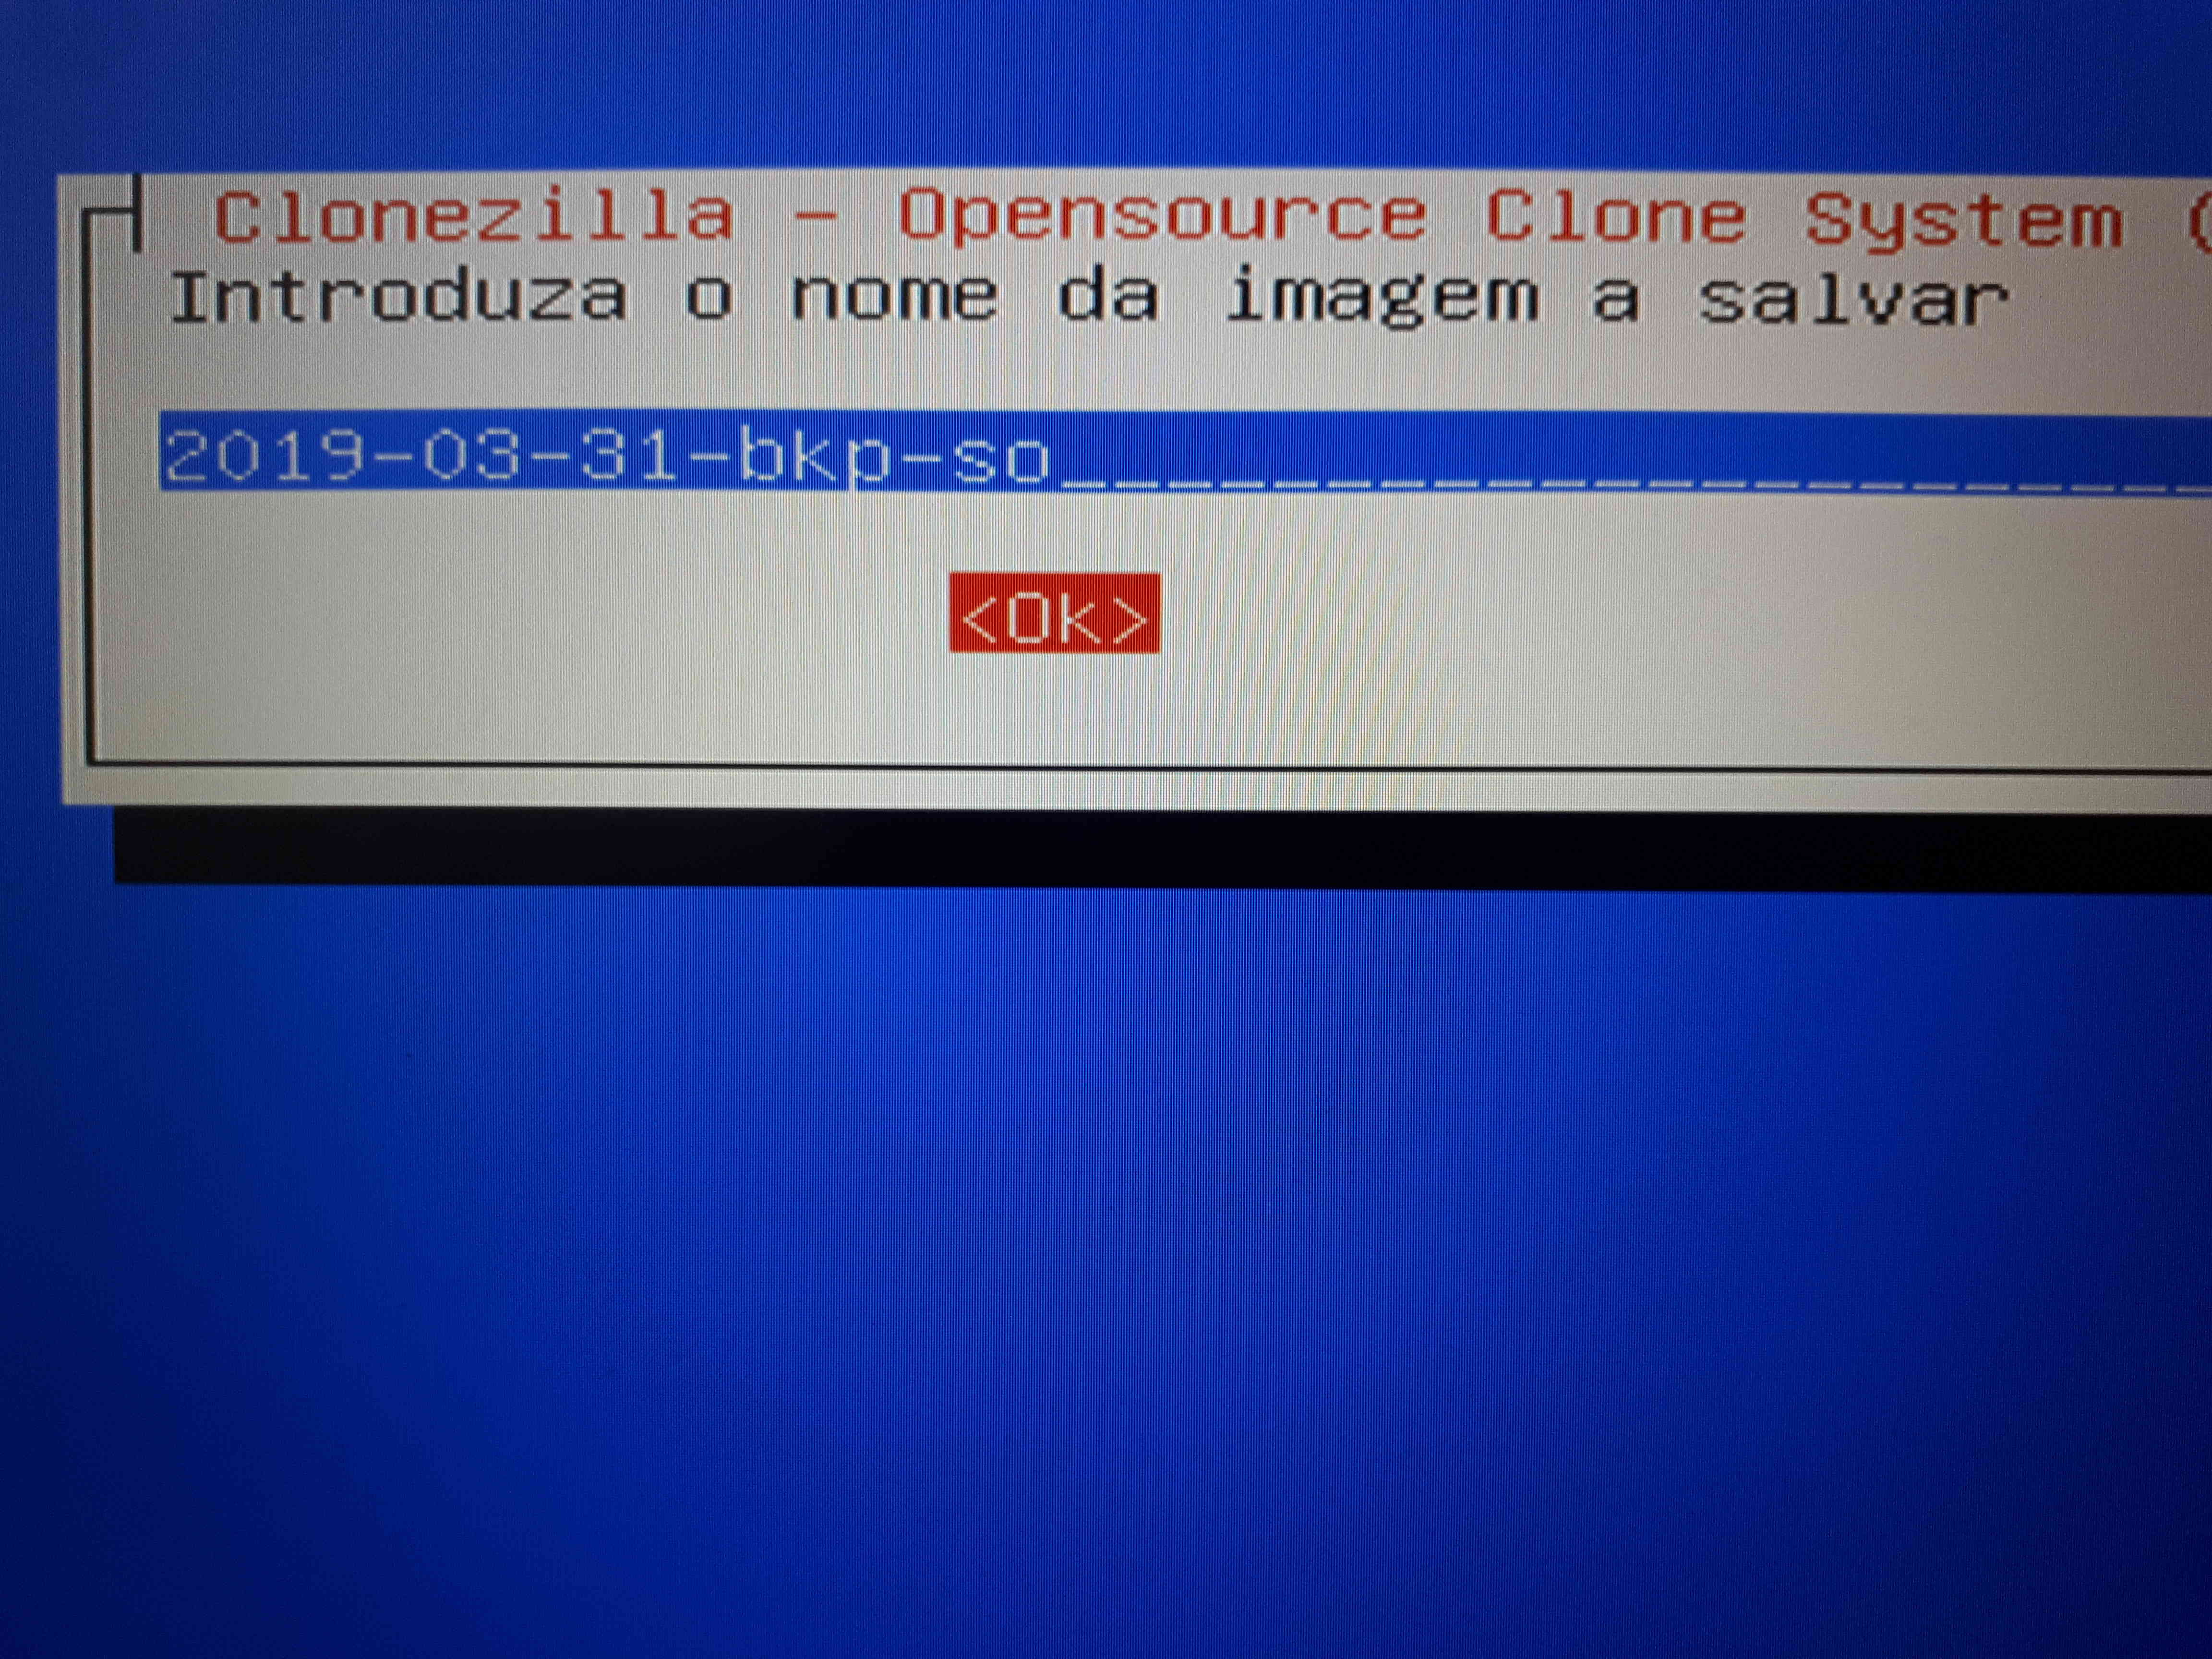
\includegraphics[width=1\linewidth]{images/backup/bkp16.jpg}
        \caption{Partições no Linux Programa GParted}
    \end{figure}
\end{frame}
\begin{frame}[plain,c]
   \frametitle{\insertsection}
    \framesubtitle{Escolhendo as partições a serem SALVAS}
    \begin{figure}[!h]
        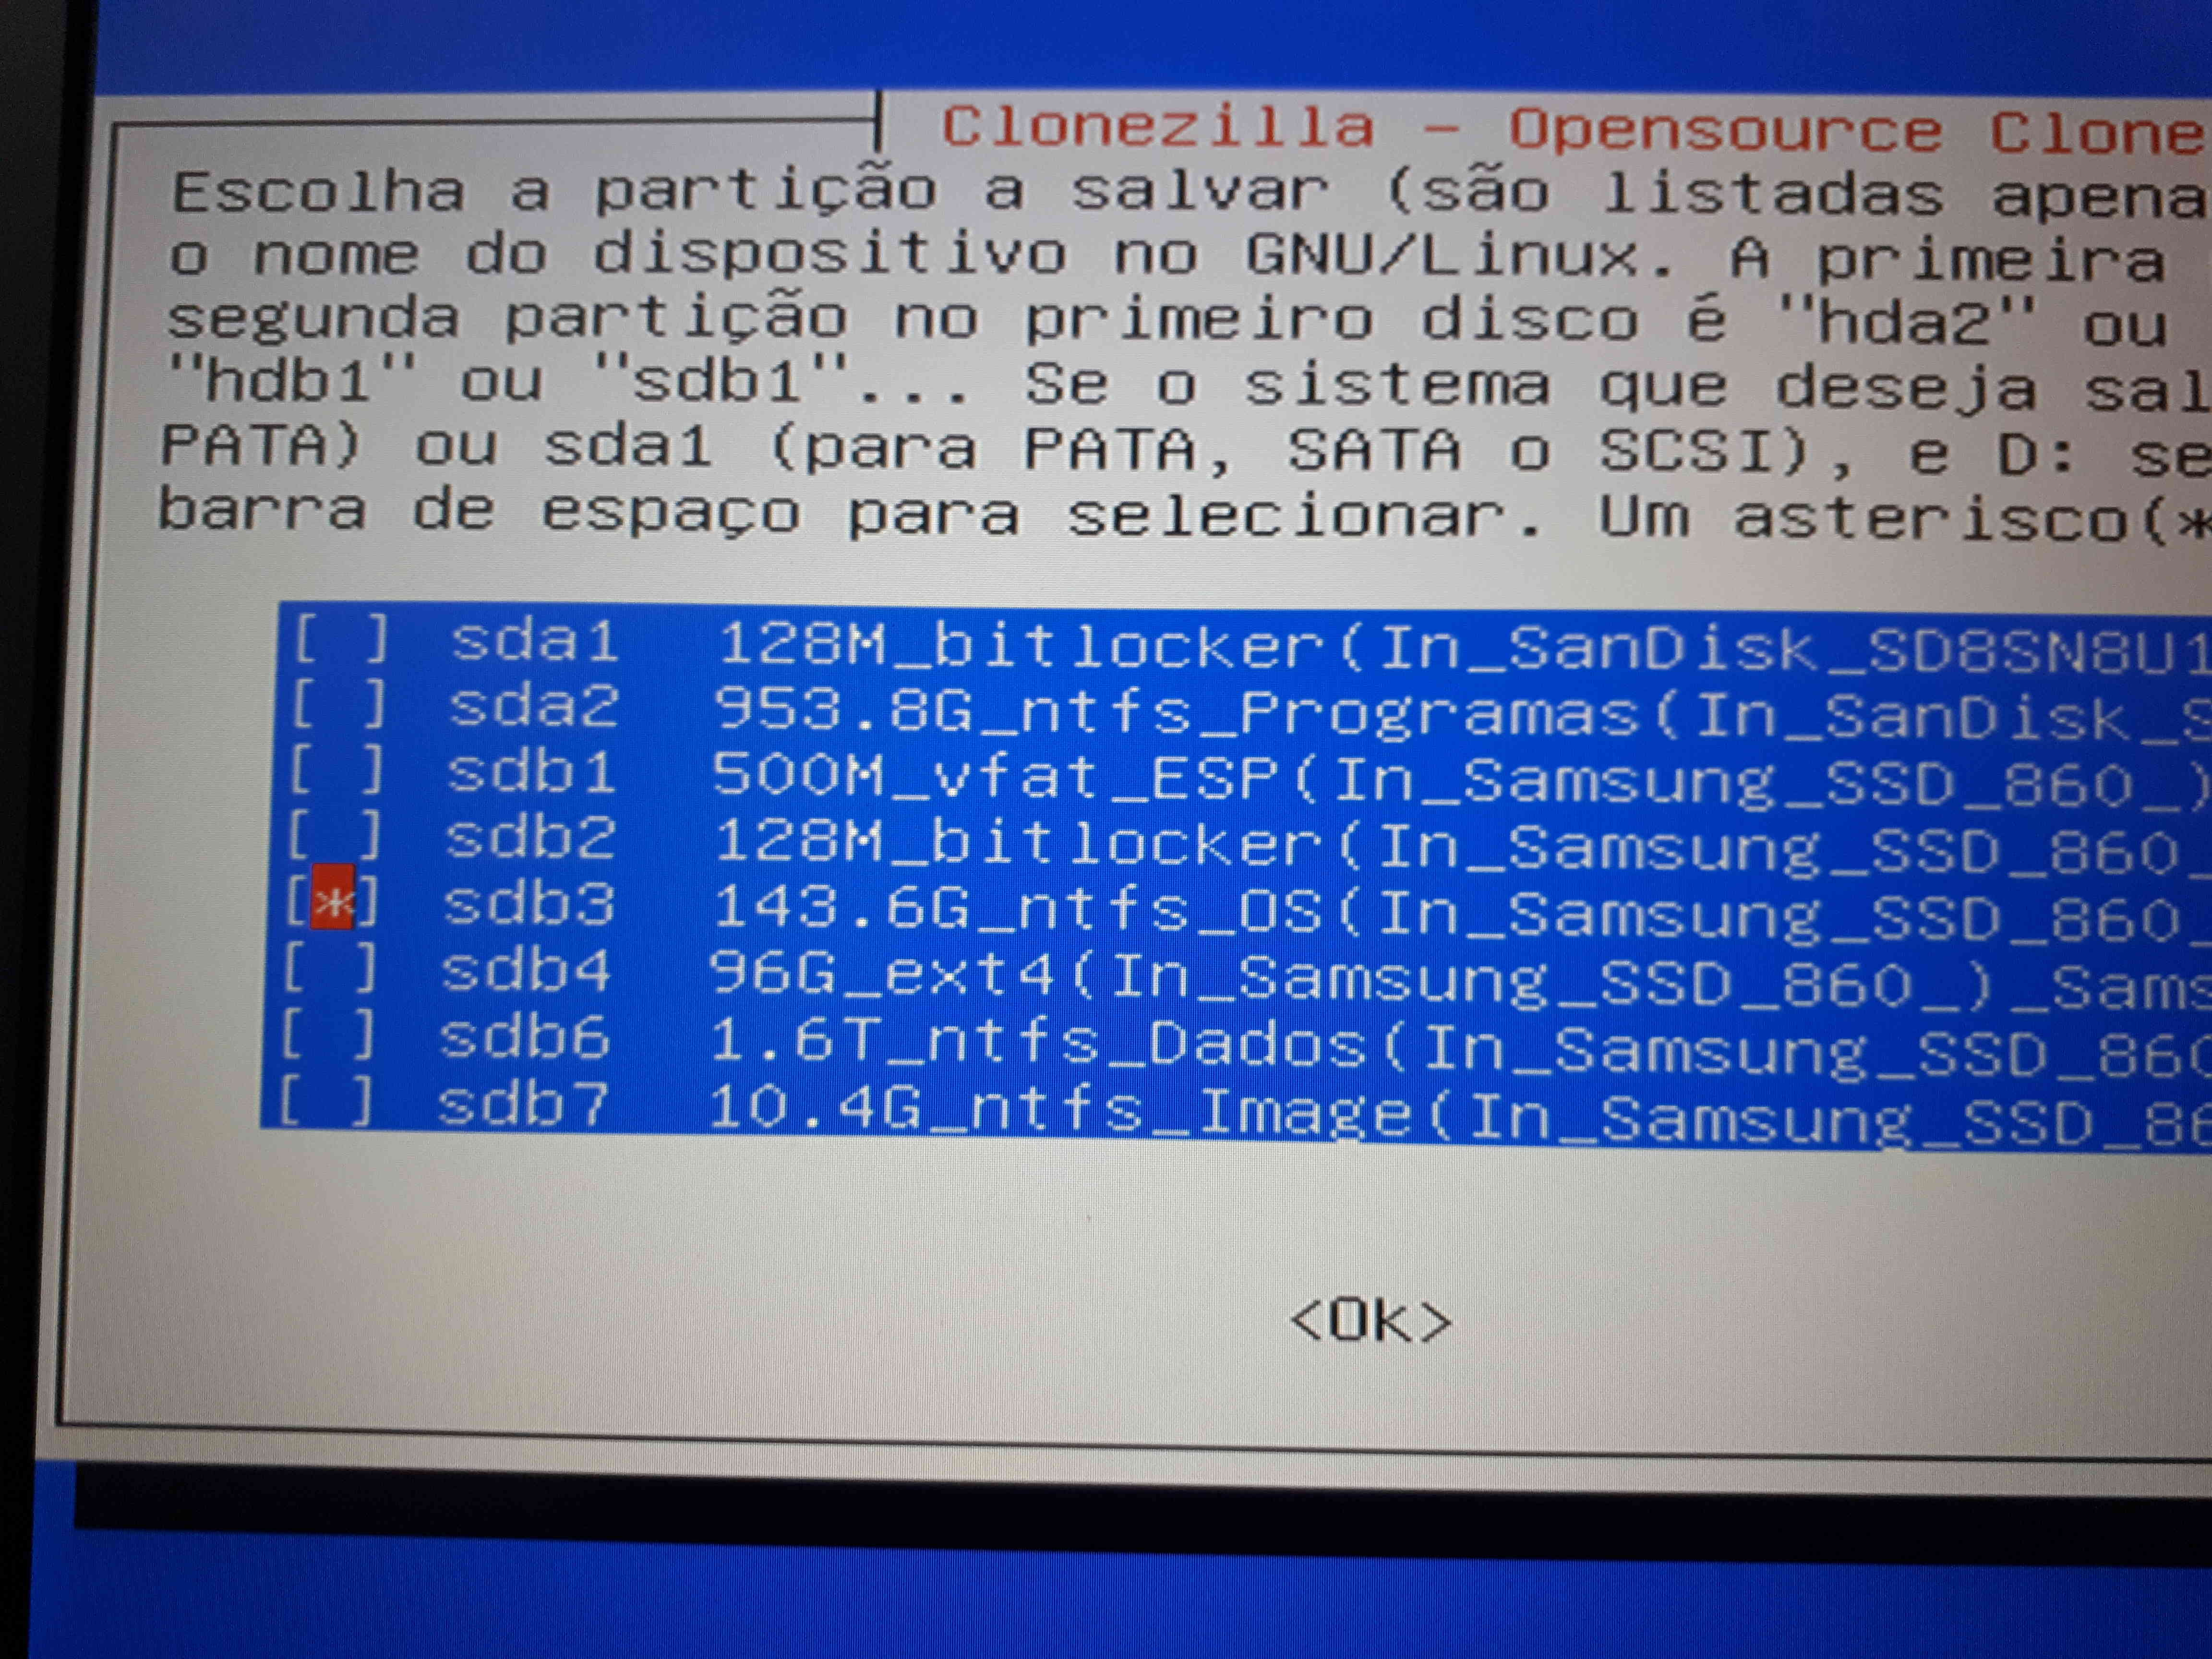
\includegraphics[width=1\linewidth]{images/backup/bkp17.jpg}
        \caption{Partições no Linux Programa GParted}
    \end{figure}
\end{frame}

\begin{frame}[plain,c]
   \frametitle{\insertsection}
    \framesubtitle{Escolhendo as partições a serem SALVAS}
    \begin{figure}[!h]
        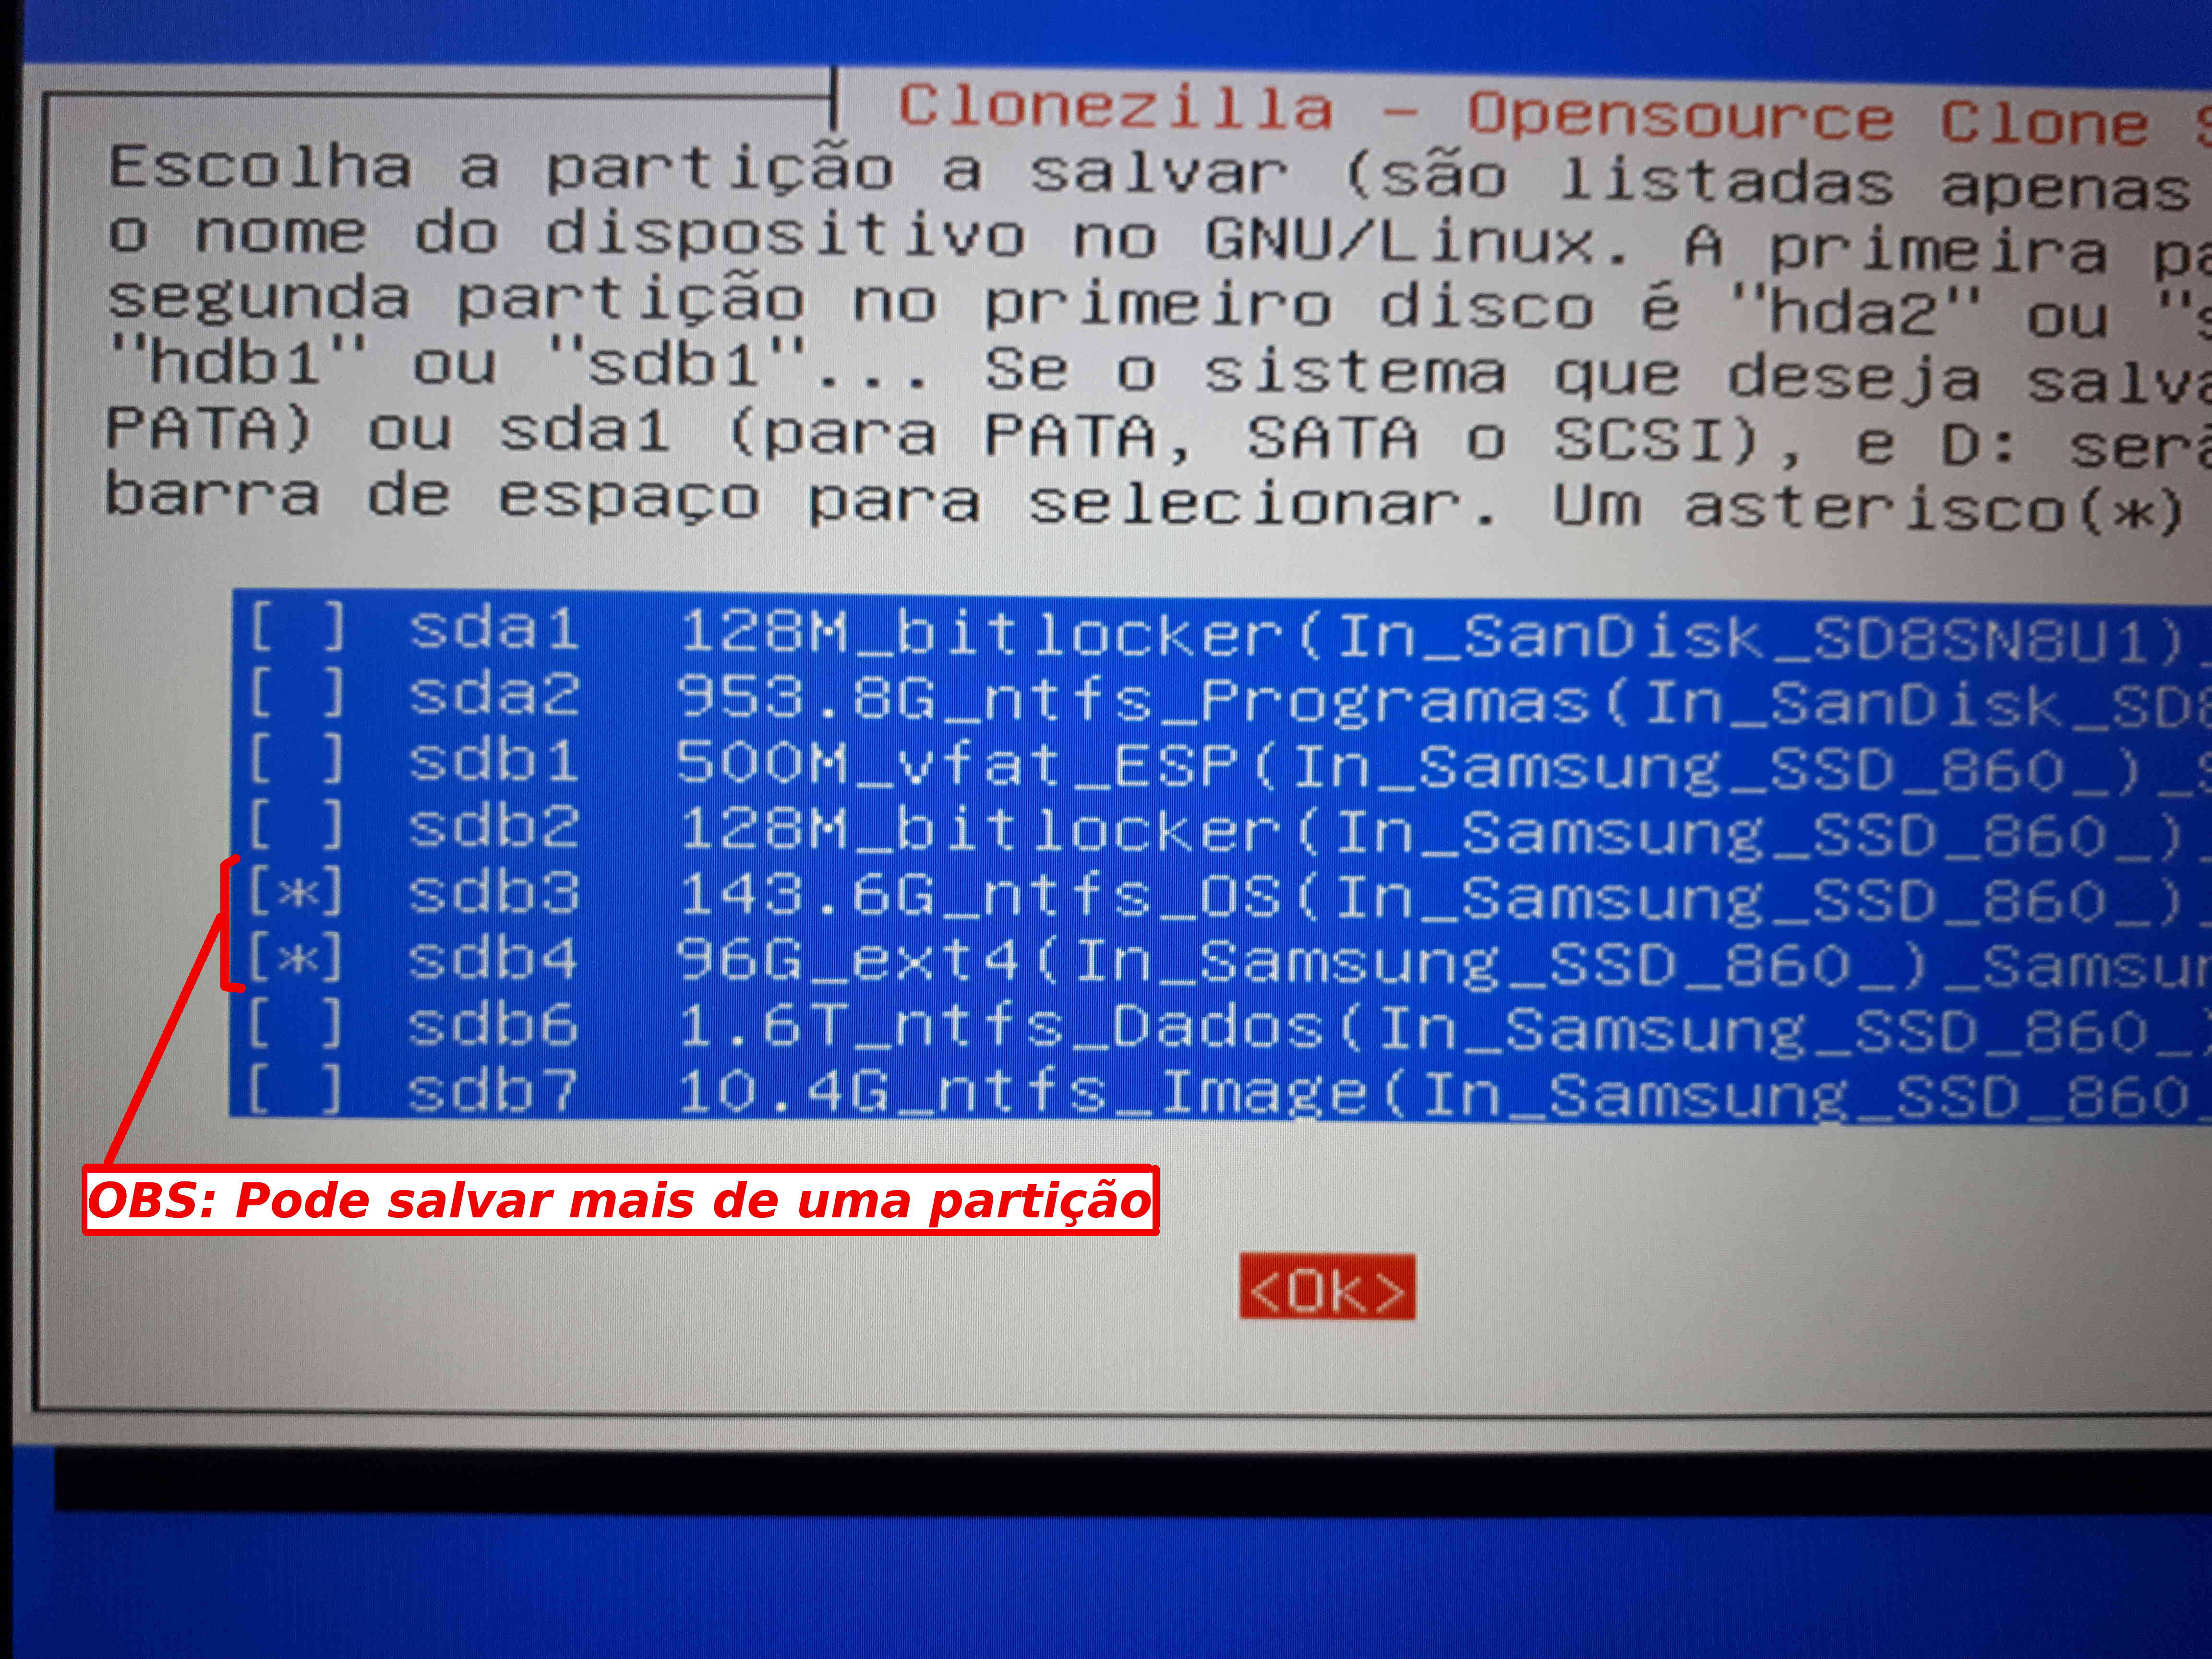
\includegraphics[width=1\linewidth]{images/backup/bkp18.jpg}
        \caption{Partições no Linux Programa GParted}
    \end{figure}
\end{frame}

\begin{frame}[plain,c]
   \frametitle{\insertsection}
    \framesubtitle{Finalizando as configuração de BACKUP}
    \begin{figure}[!h]
        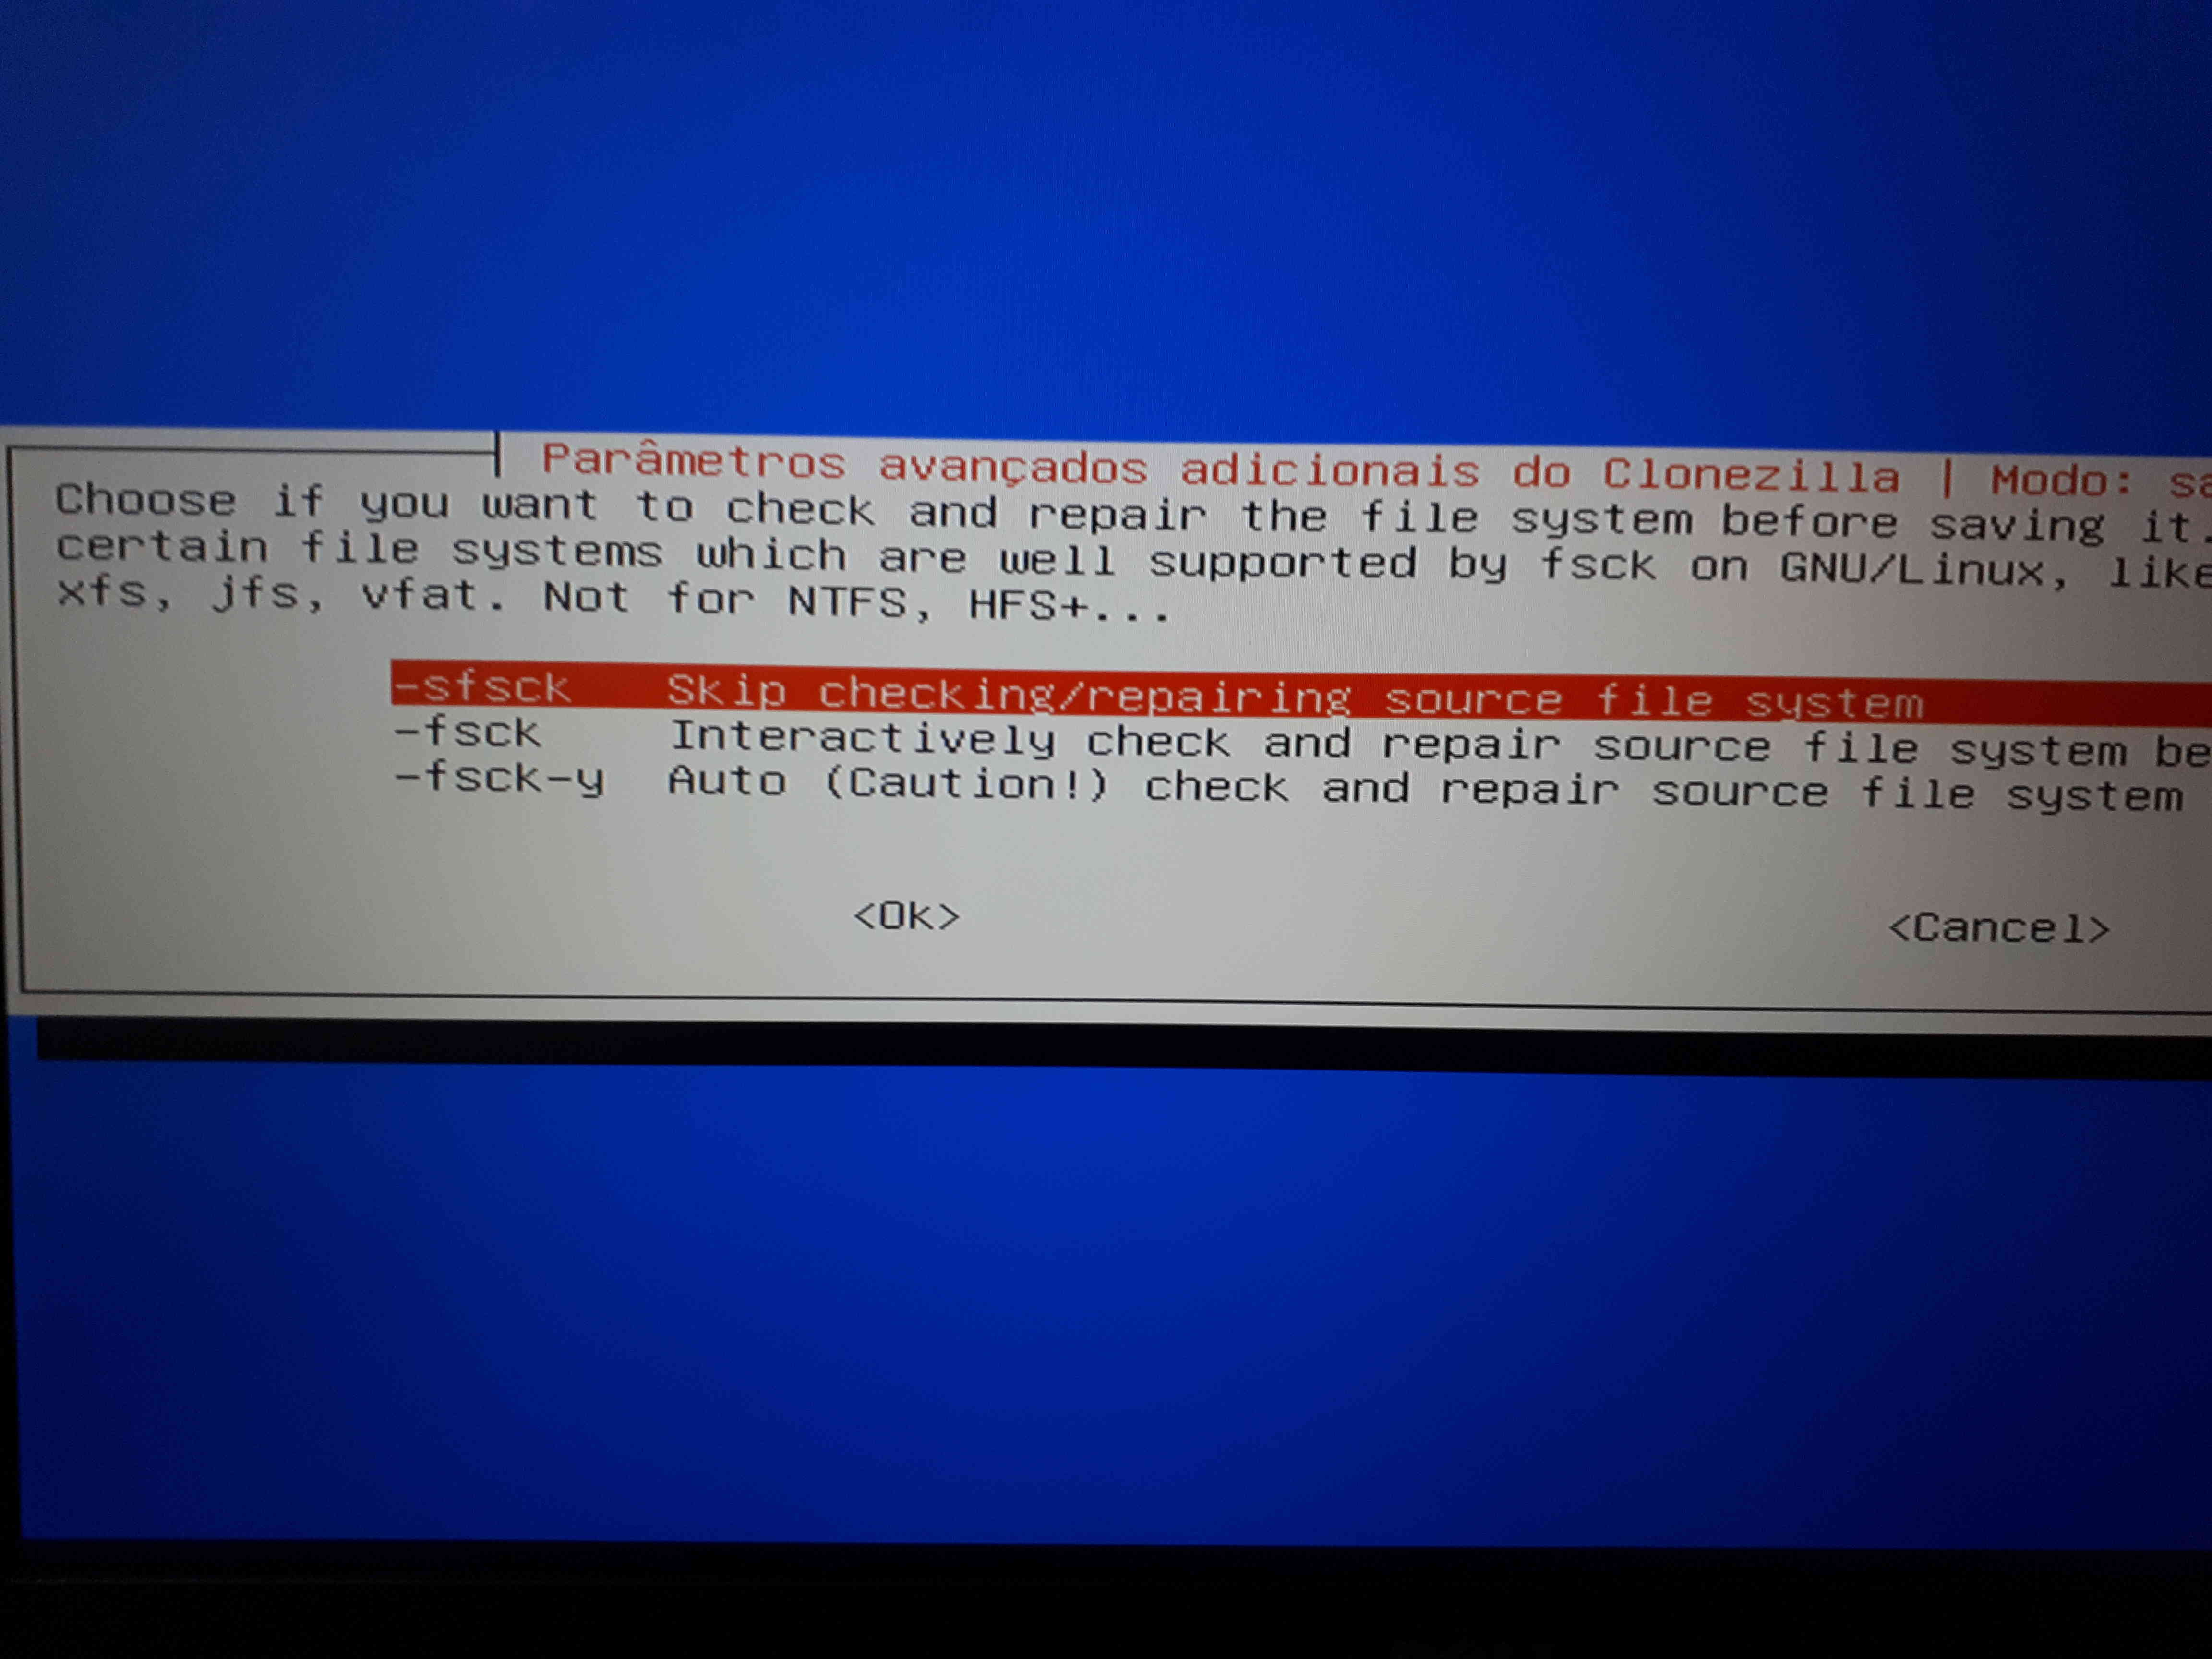
\includegraphics[width=1\linewidth]{images/backup/bkp19.jpg}
        \caption{Partições no Linux Programa GParted}
    \end{figure}
\end{frame}	

\begin{frame}[plain,c]
   \frametitle{\insertsection}
    \framesubtitle{Finalizando as configuração de BACKUP}
    \begin{figure}[!h]
        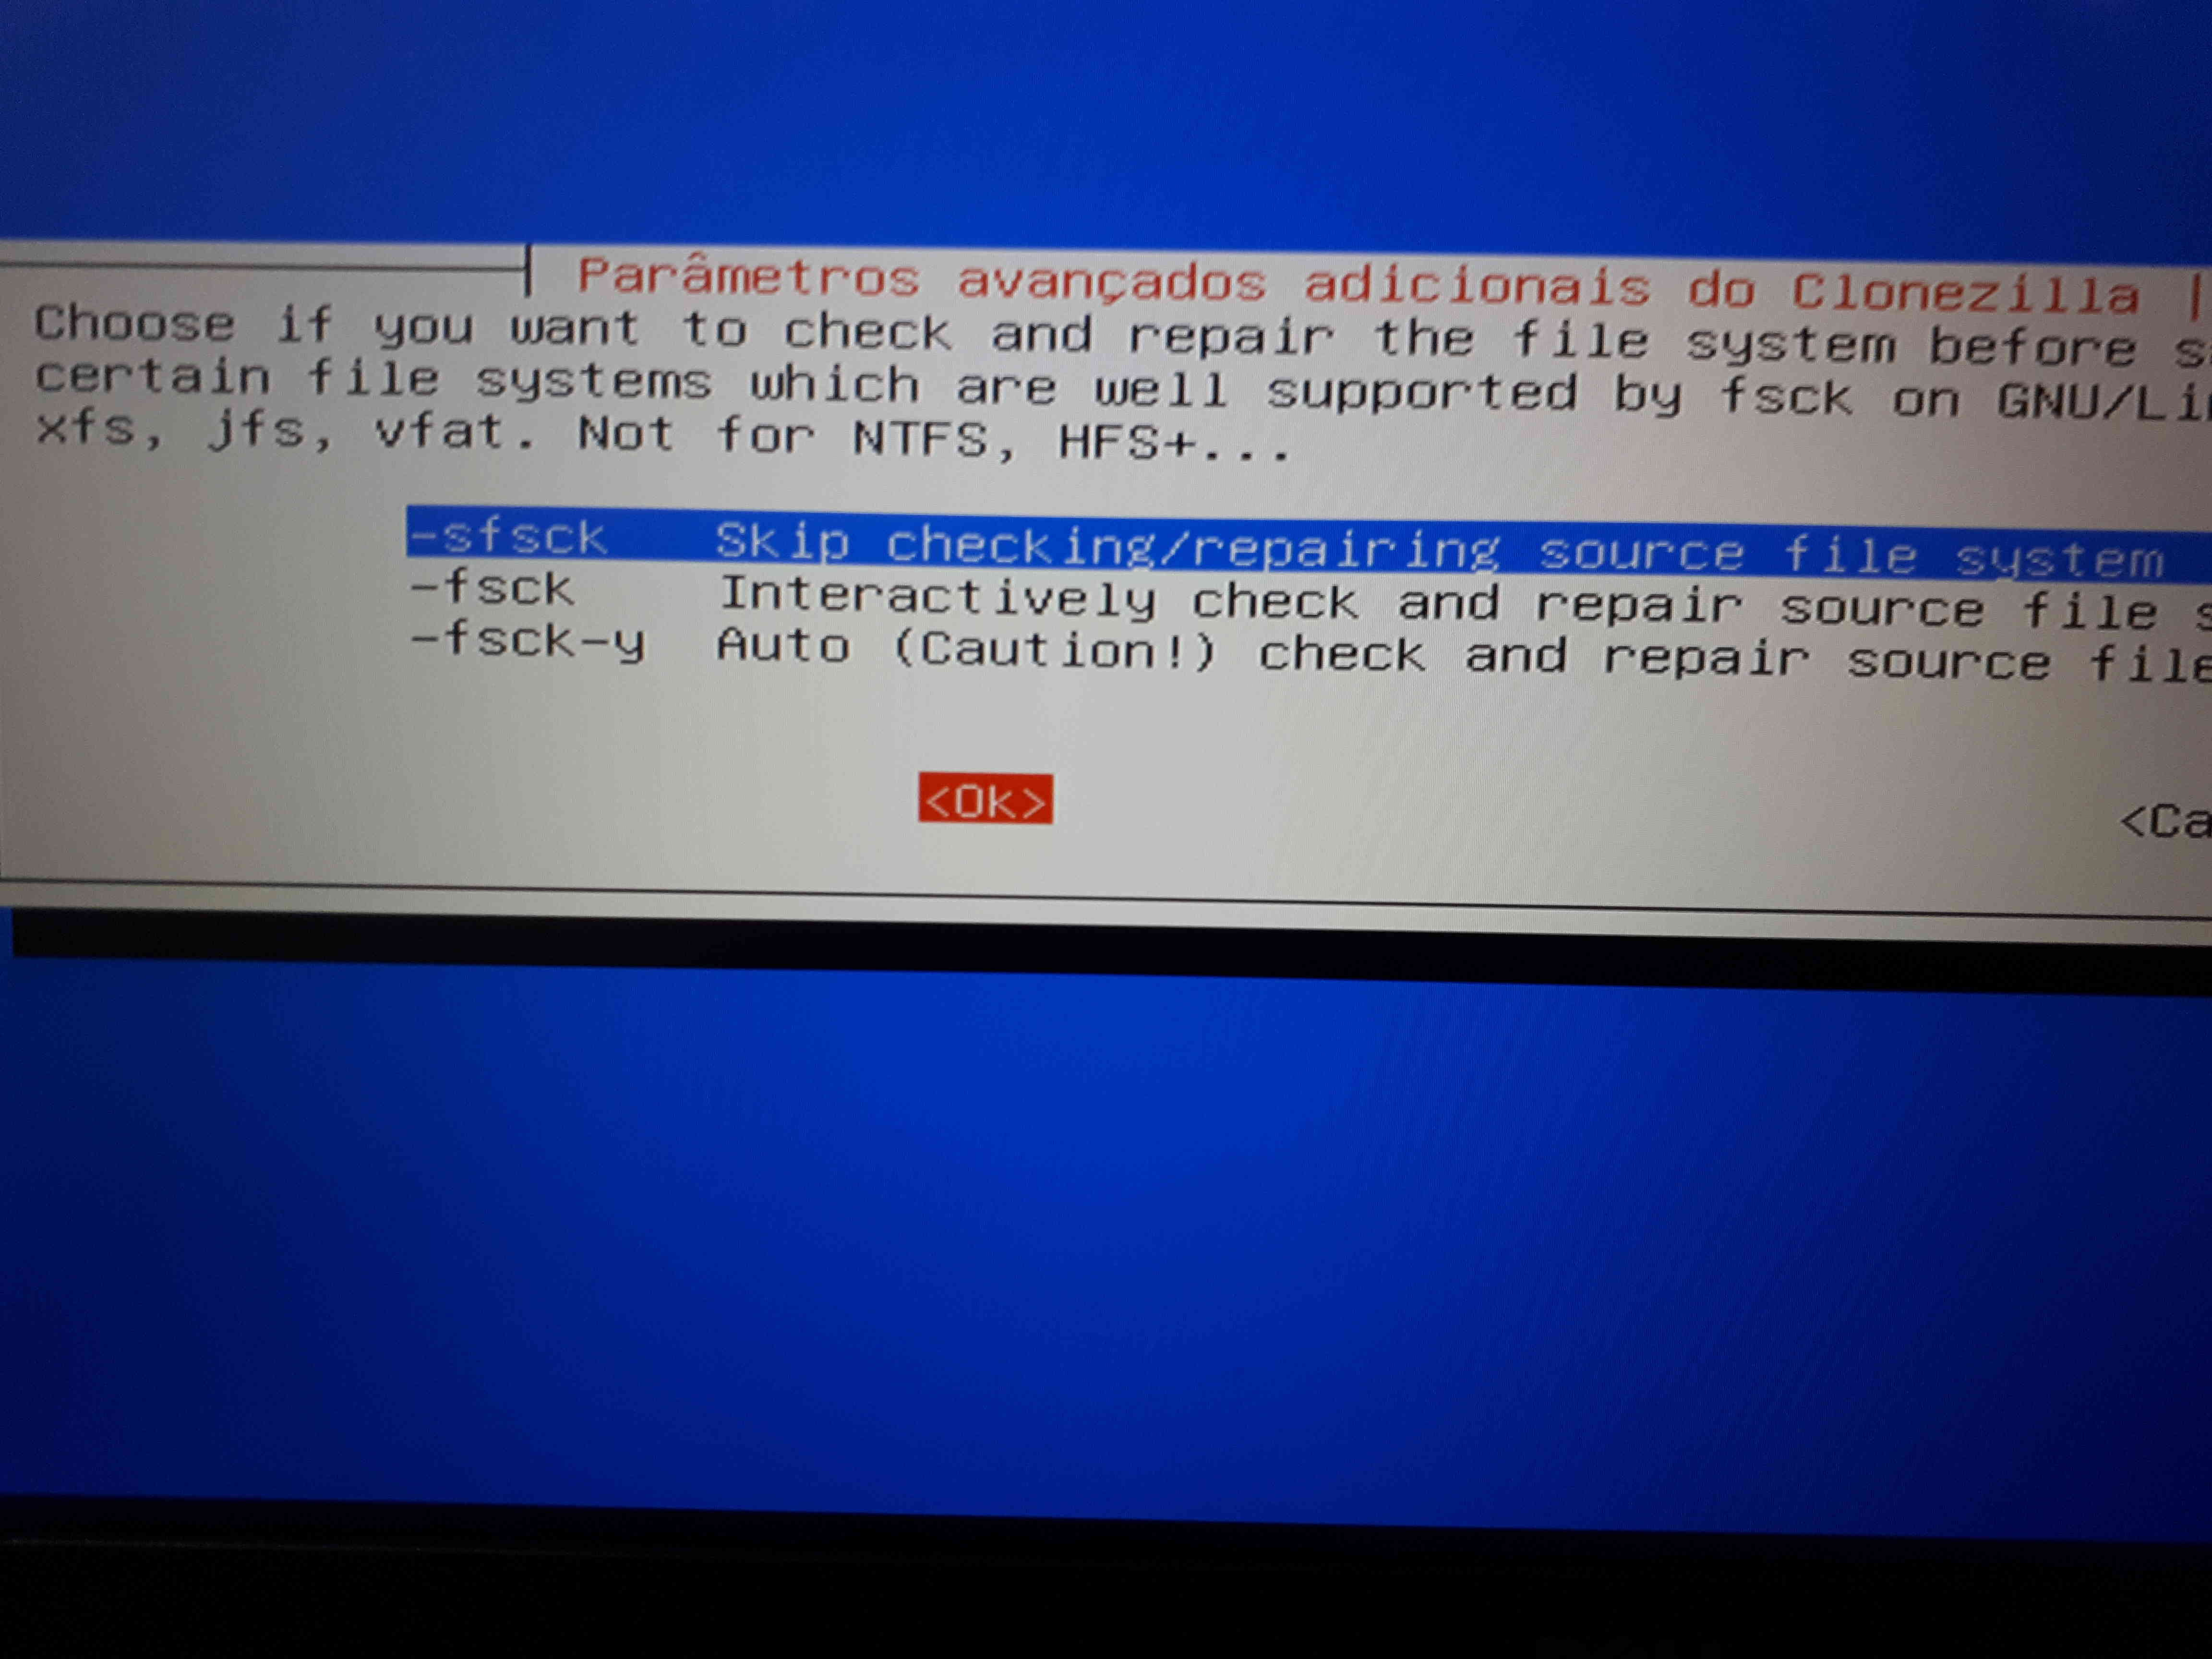
\includegraphics[width=1\linewidth]{images/backup/bkp20.jpg}
        \caption{Partições no Linux Programa GParted}
    \end{figure}
\end{frame}	
\begin{frame}[plain,c]
   \frametitle{\insertsection}
    \framesubtitle{Finalizando as configuração de BACKUP}
    \begin{figure}[!h]
        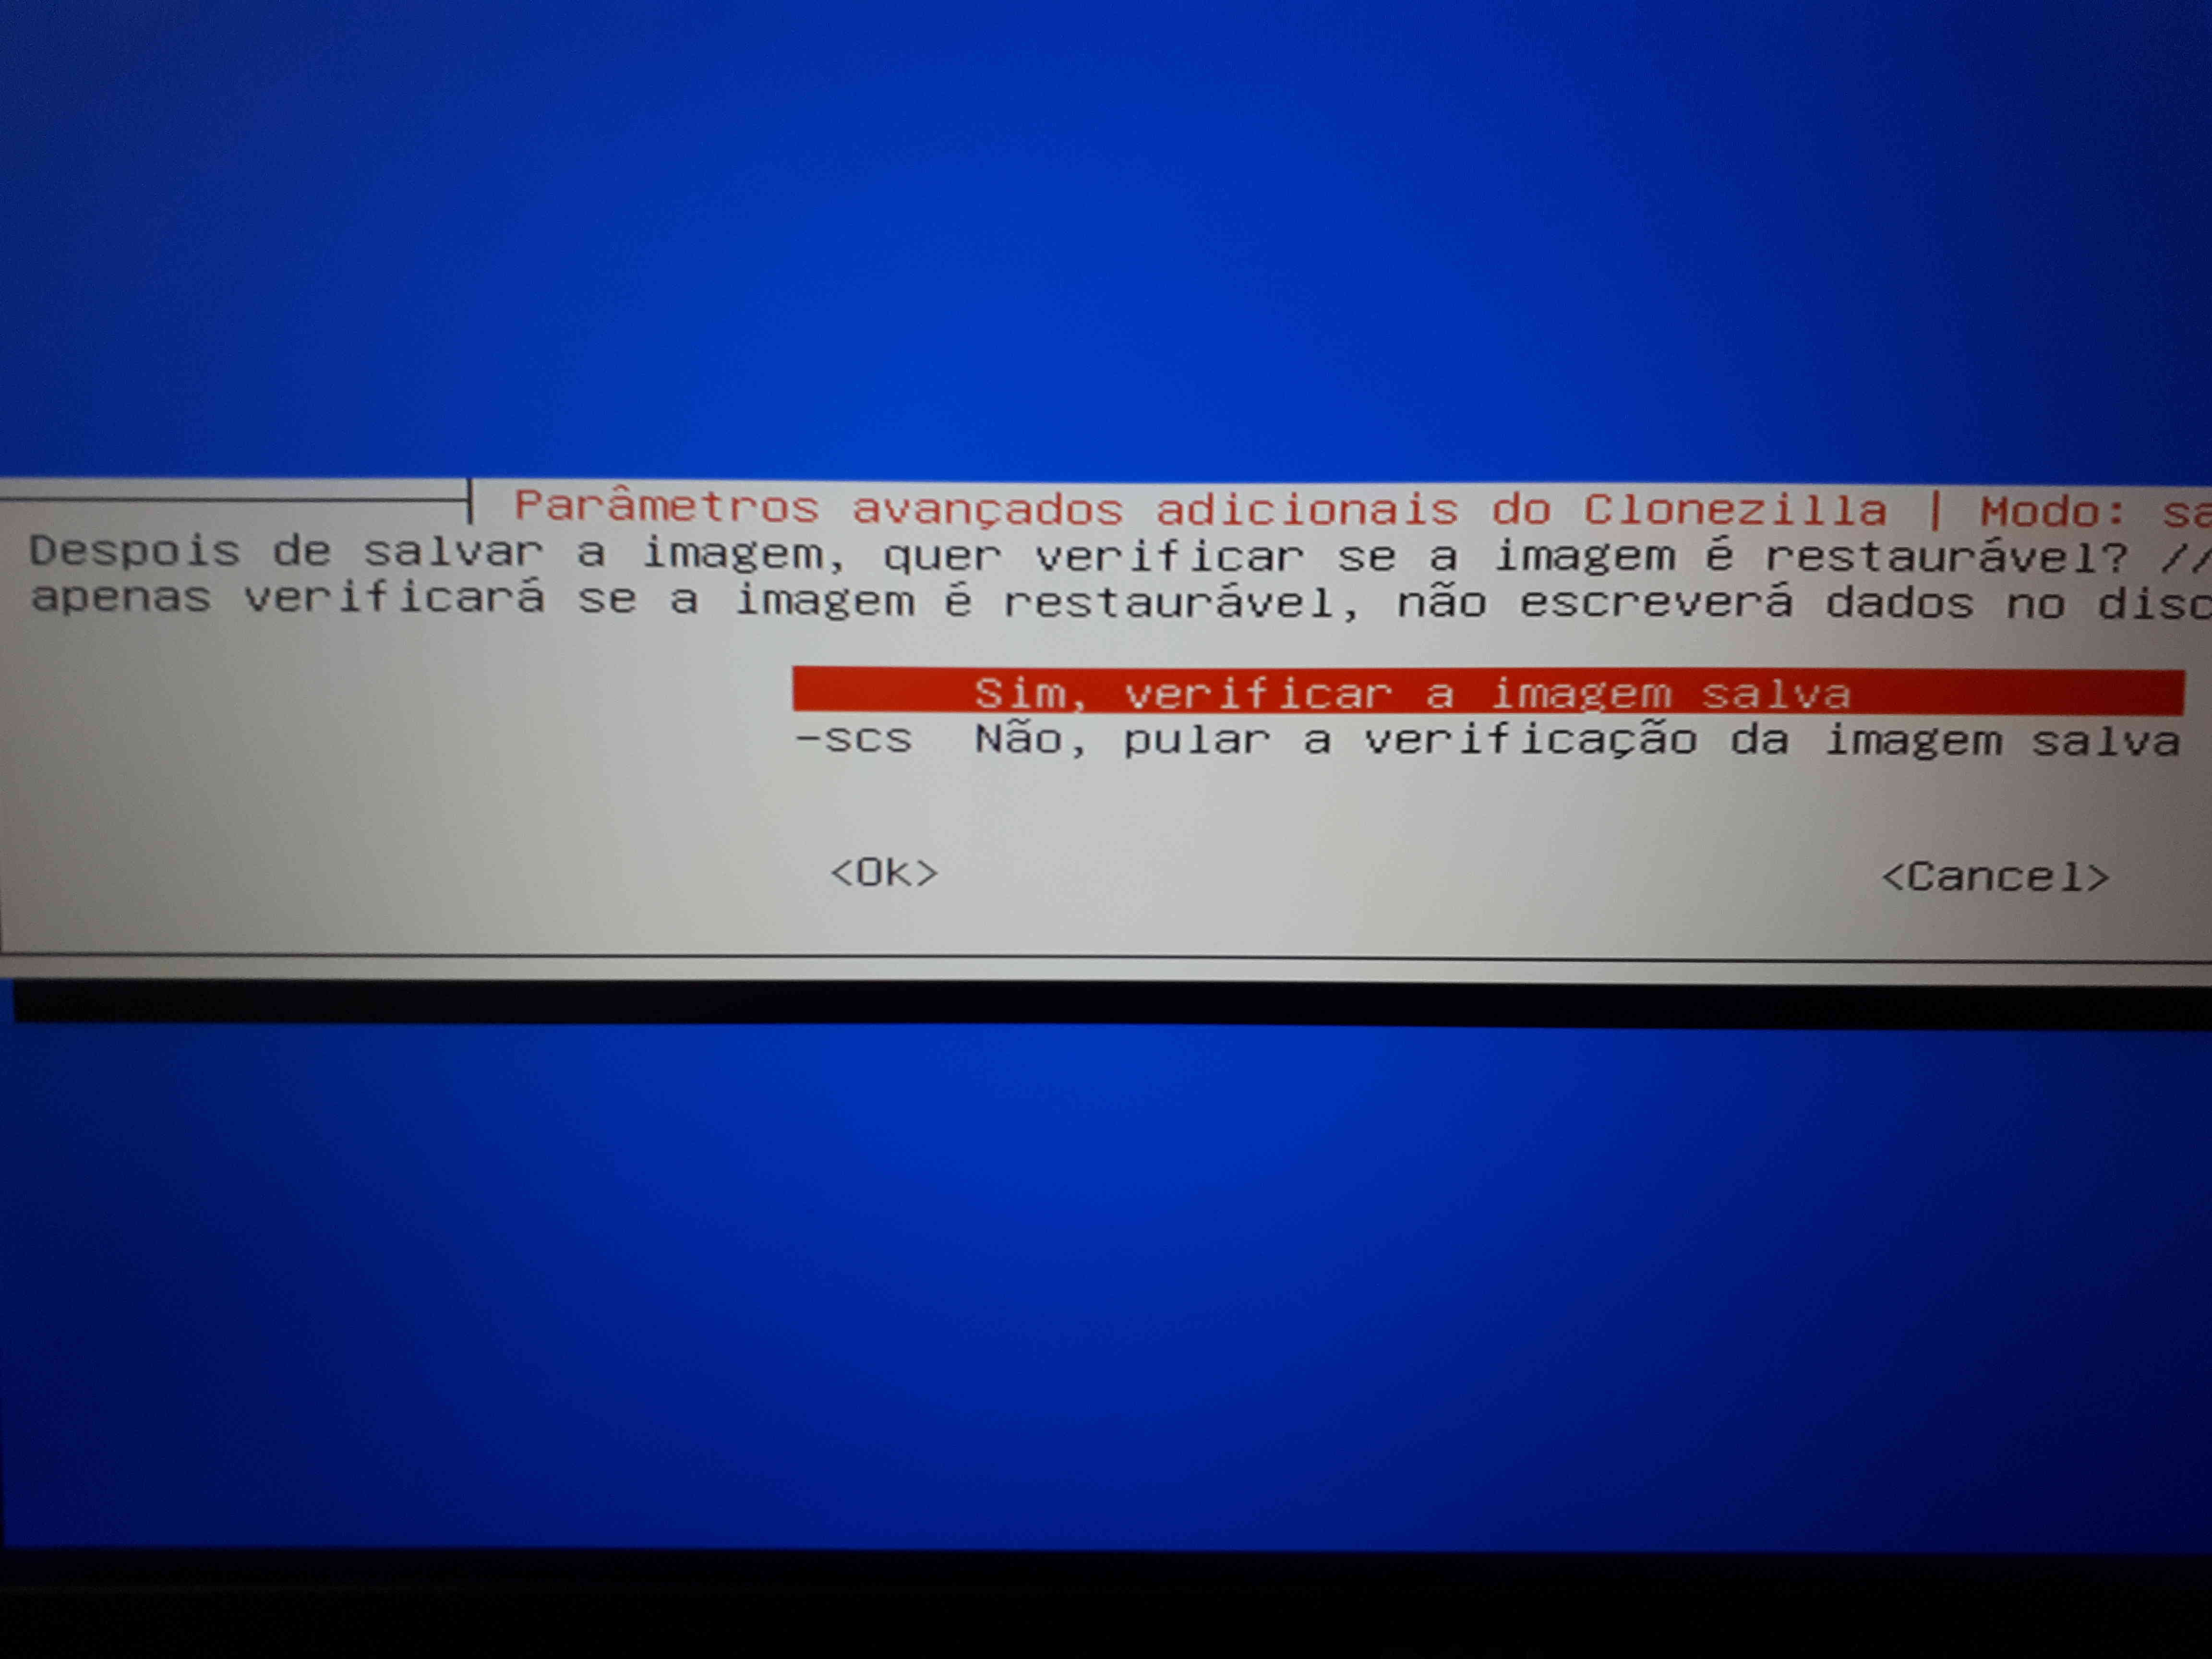
\includegraphics[width=1\linewidth]{images/backup/bkp21.jpg}
        \caption{Partições no Linux Programa GParted}
    \end{figure}
\end{frame}	
\begin{frame}[plain,c]
   \frametitle{\insertsection}
    \framesubtitle{Finalizando as configuração de BACKUP}
    \begin{figure}[!h]
        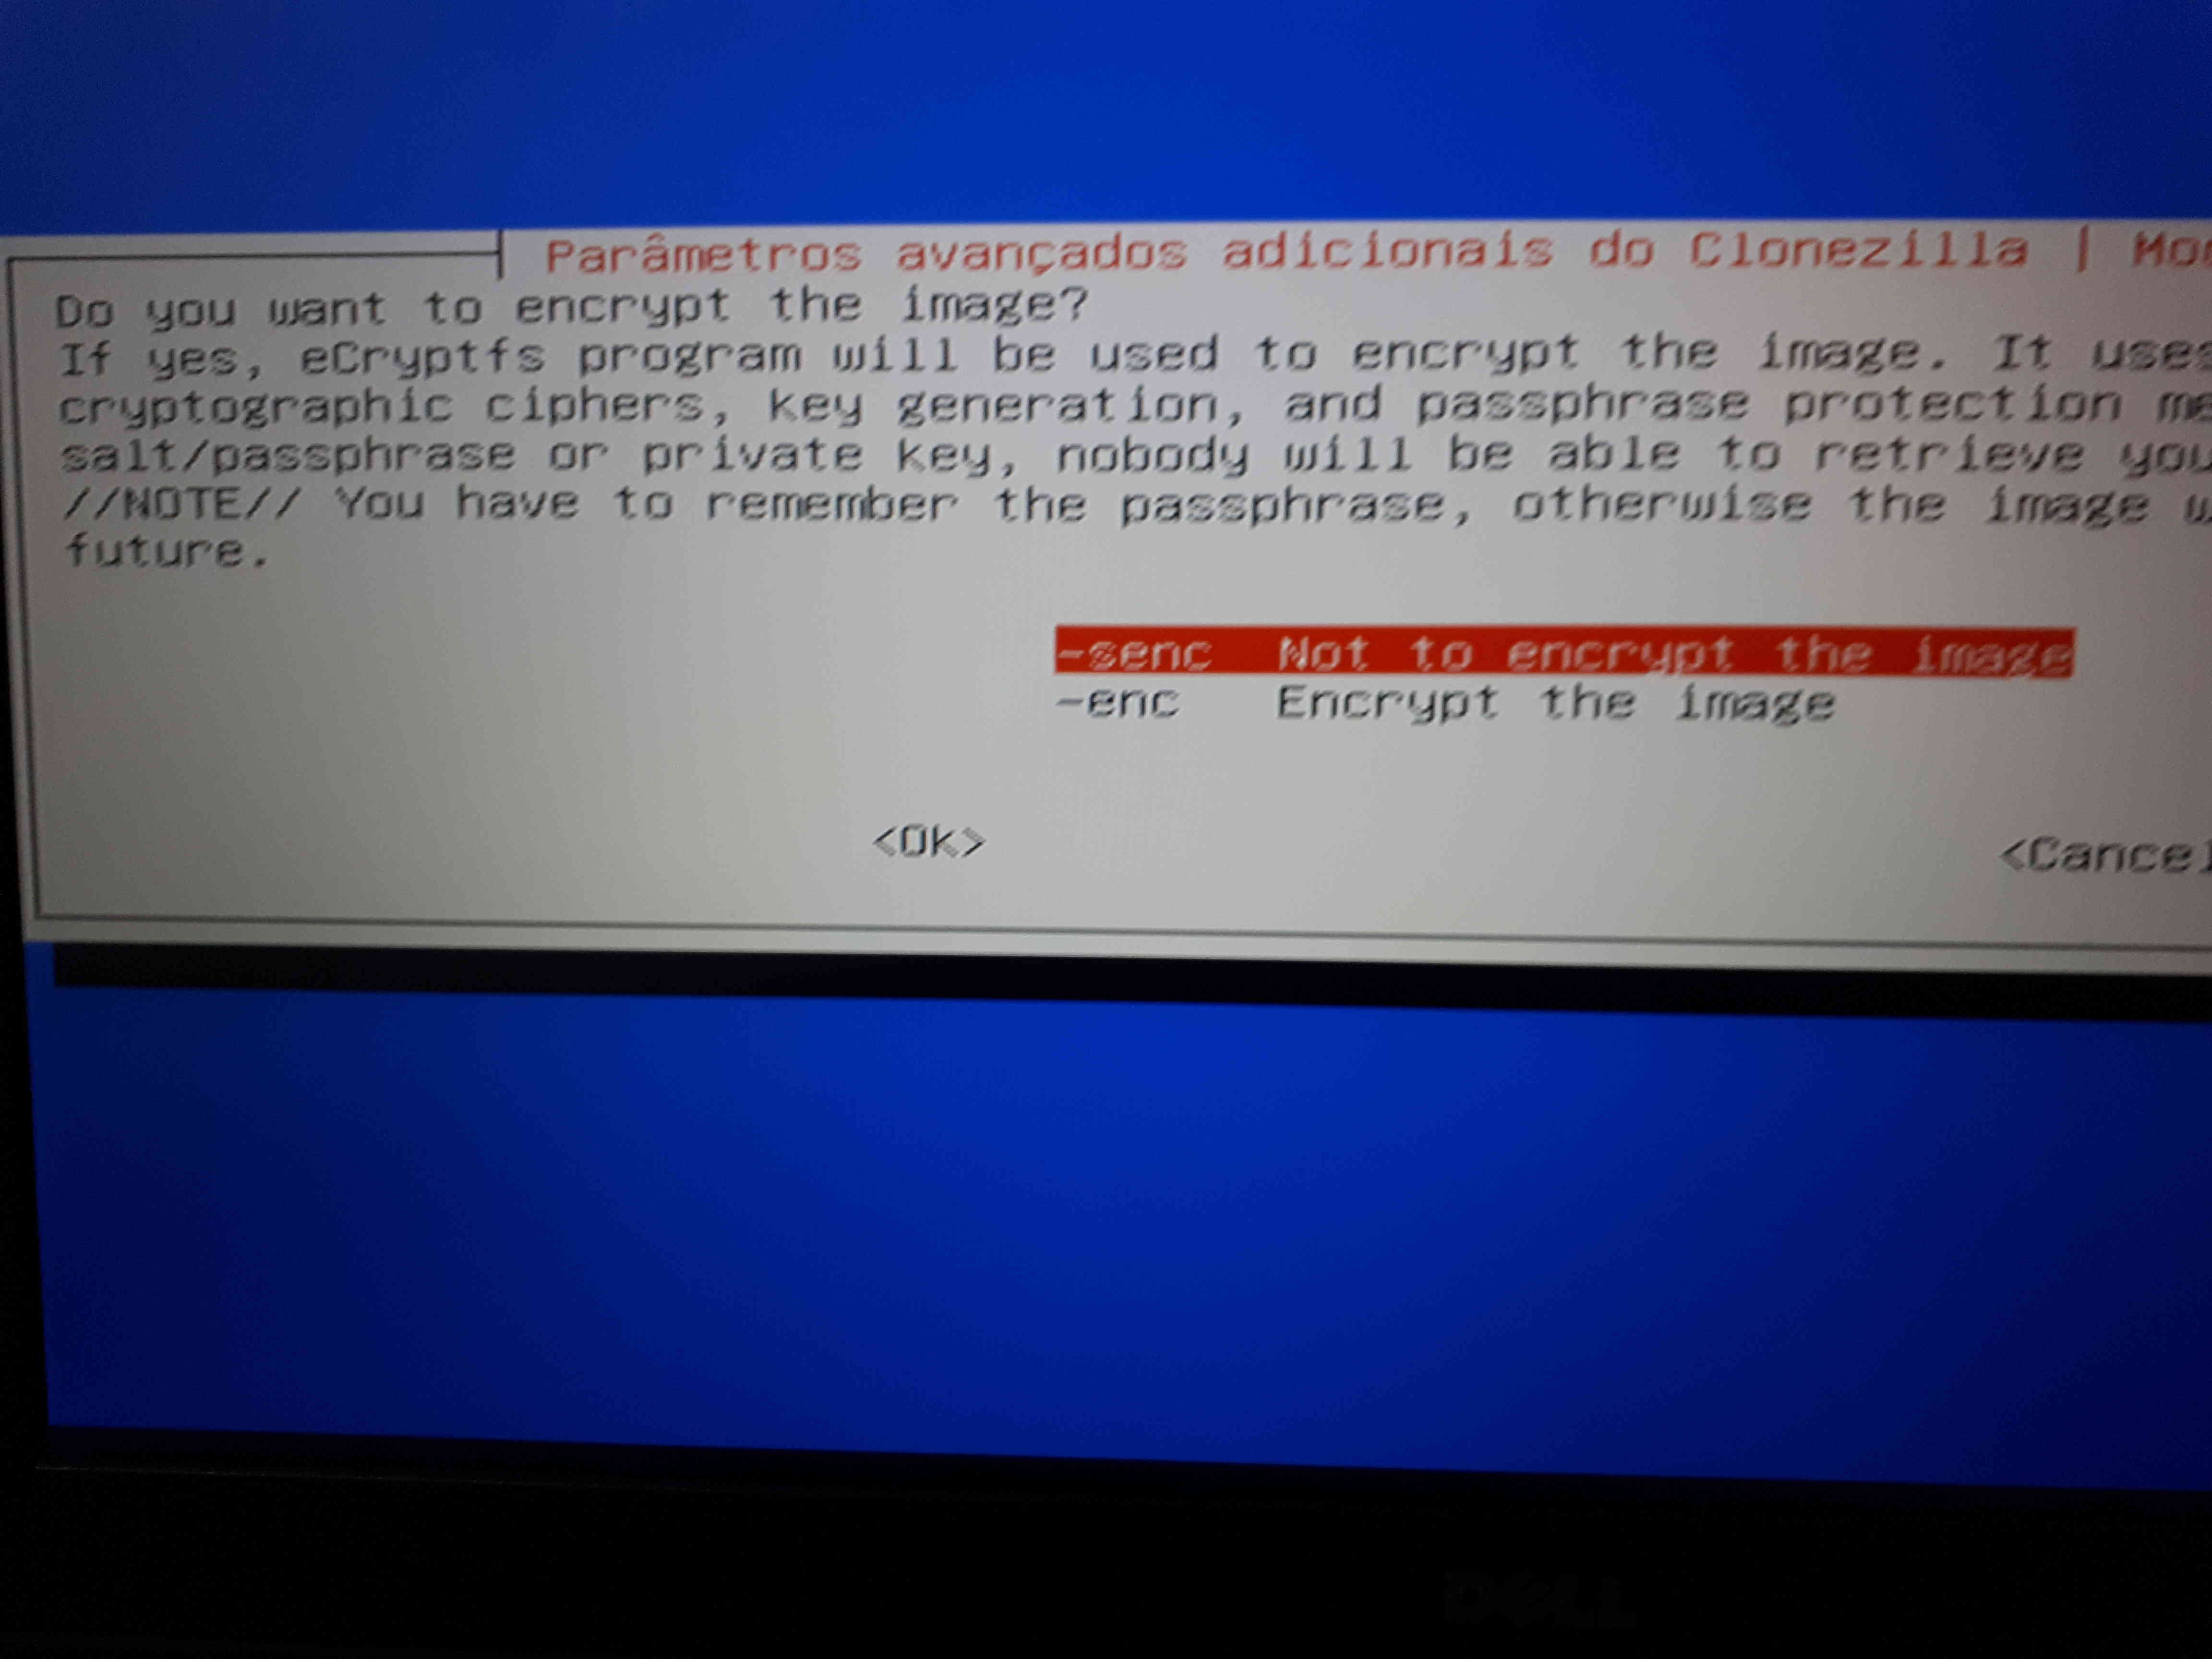
\includegraphics[width=1\linewidth]{images/backup/bkp22.jpg}
        \caption{Partições no Linux Programa GParted}
    \end{figure}
\end{frame}	
\begin{frame}[plain,c]
   \frametitle{\insertsection}
    \framesubtitle{Finalizando as configuração de BACKUP}
    \begin{figure}[!h]
        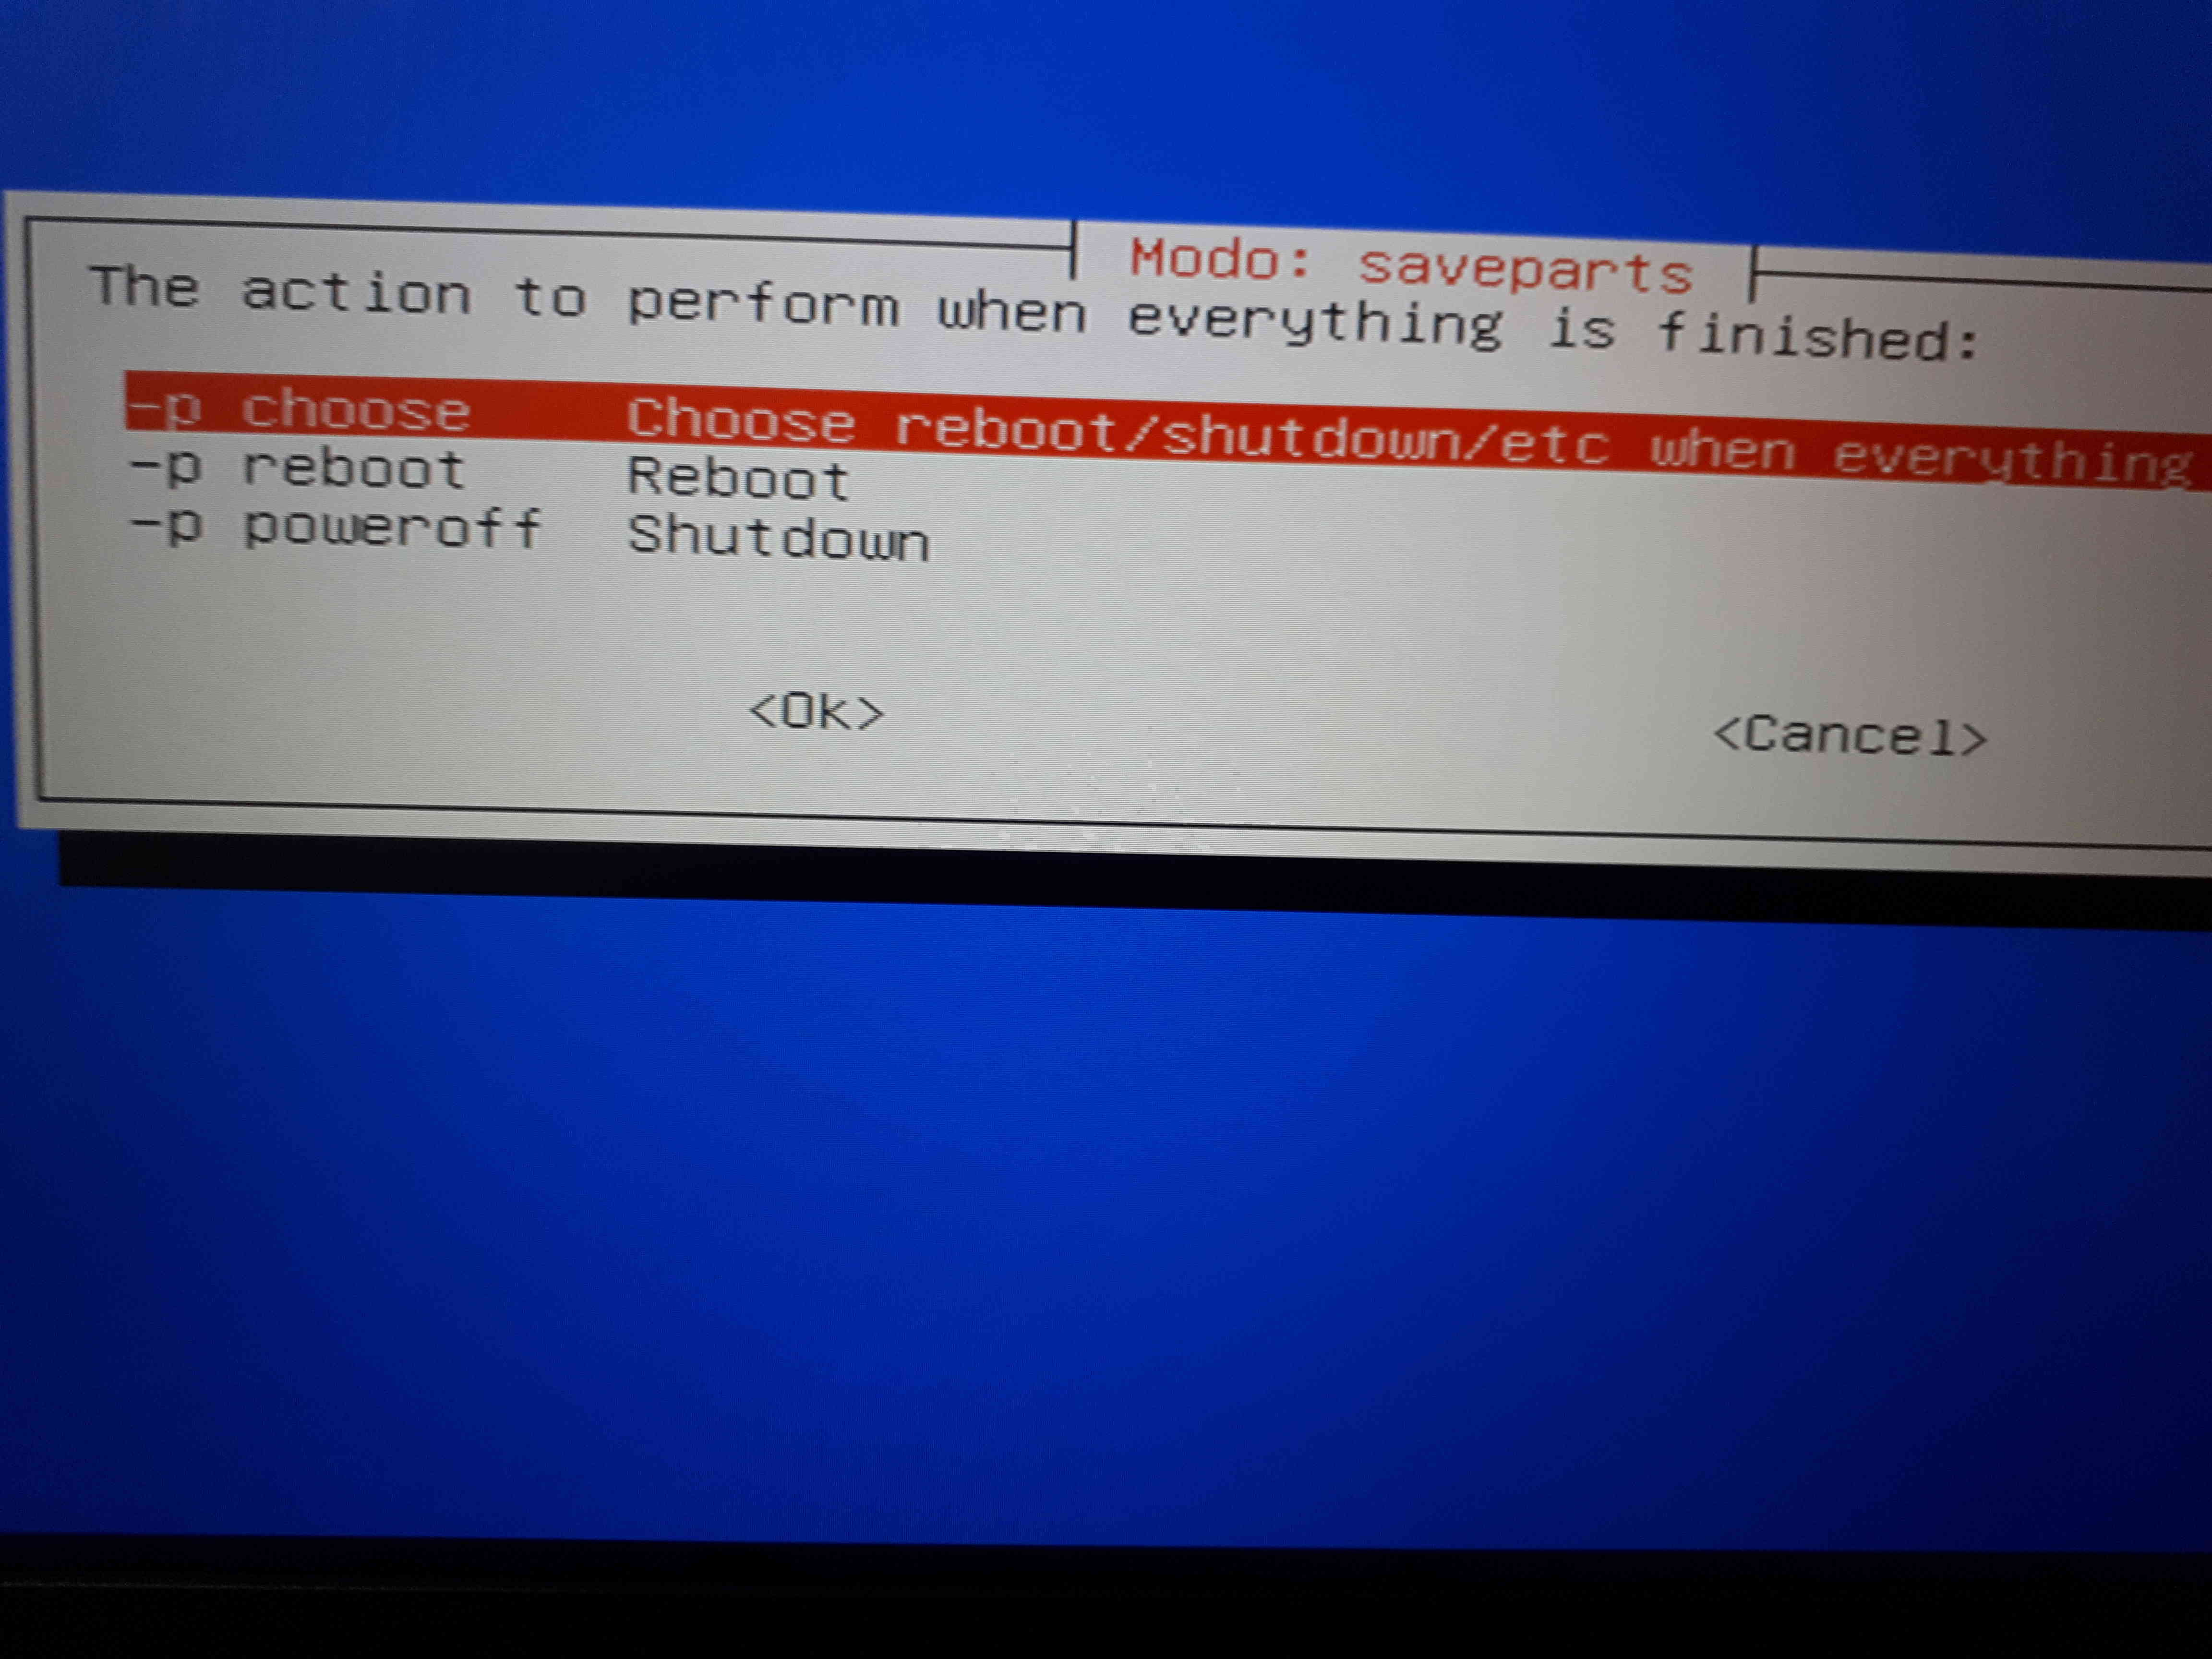
\includegraphics[width=1\linewidth]{images/backup/bkp23.jpg}
        \caption{Partições no Linux Programa GParted}
    \end{figure}
\end{frame}	

\begin{frame}[plain,c]
   \frametitle{\insertsection}
    \framesubtitle{Finalizando as configuração de BACKUP}
    \begin{figure}[!h]
        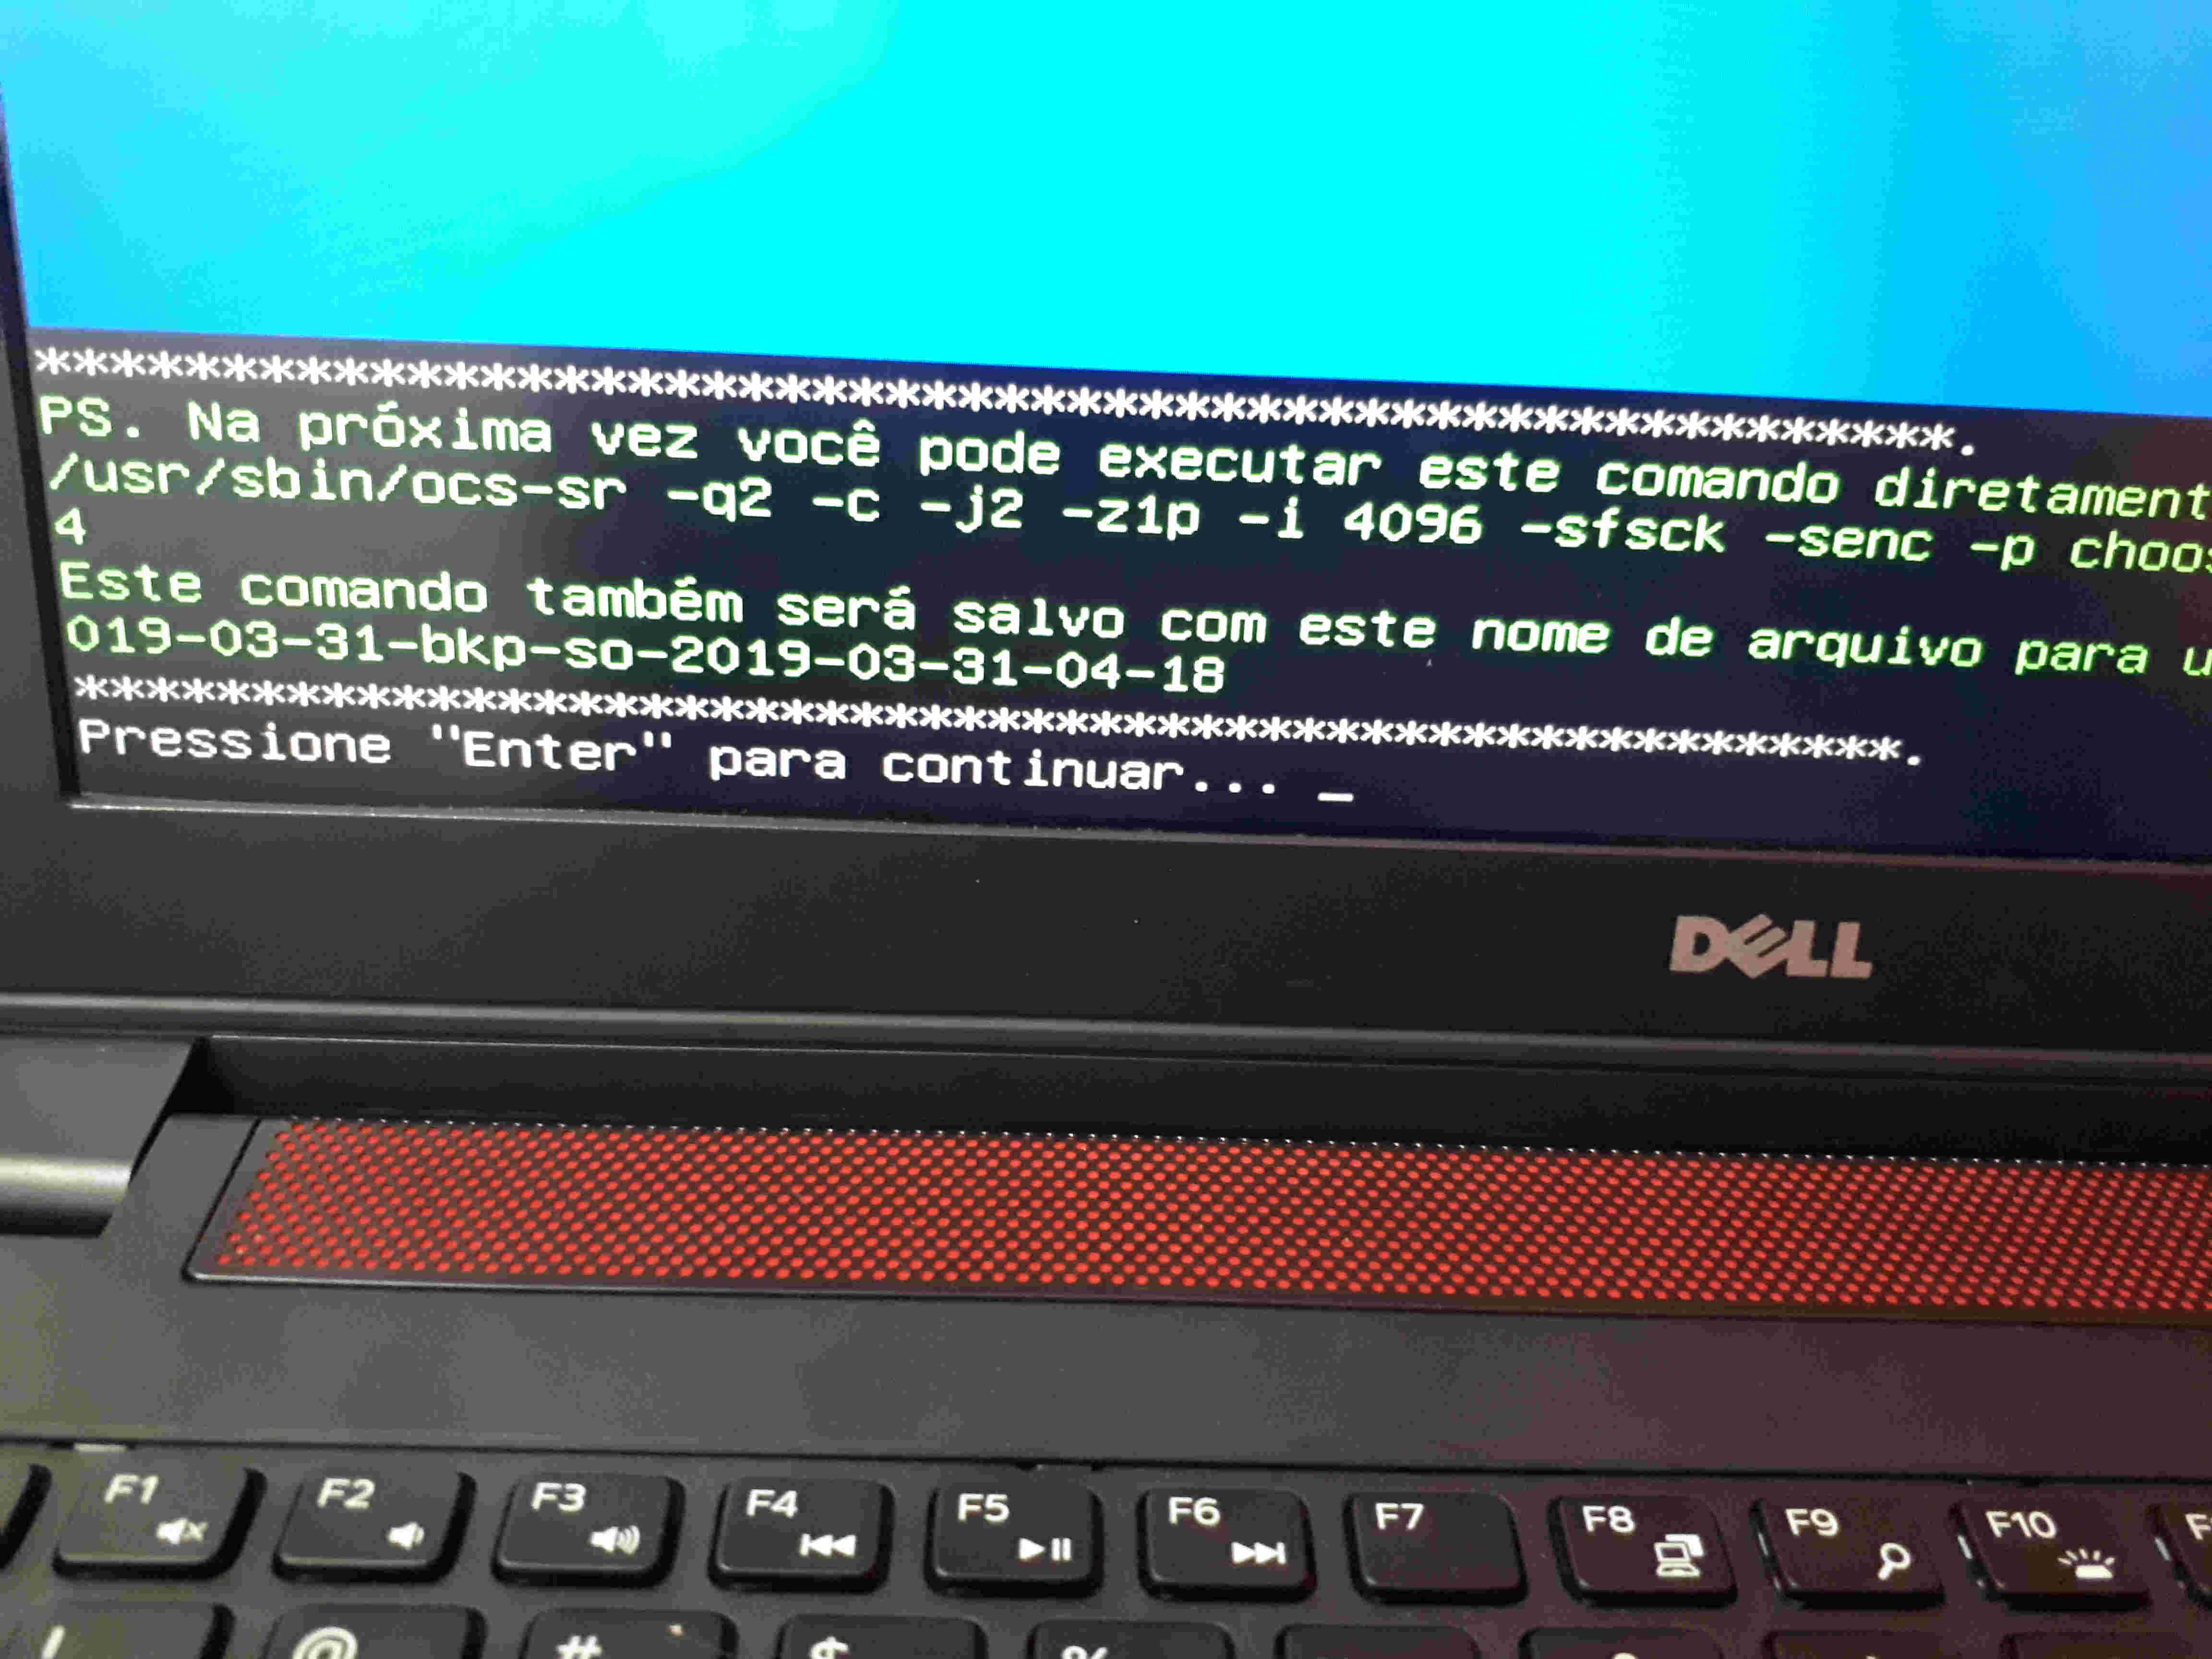
\includegraphics[width=1\linewidth]{images/backup/bkp24.jpg}
        \caption{Partições no Linux Programa GParted}
    \end{figure}
\end{frame}	

\begin{frame}[plain,c]
   \frametitle{\insertsection}
    \framesubtitle{Confirmação para iniciar o BACKUP}
    \begin{figure}[!h]
        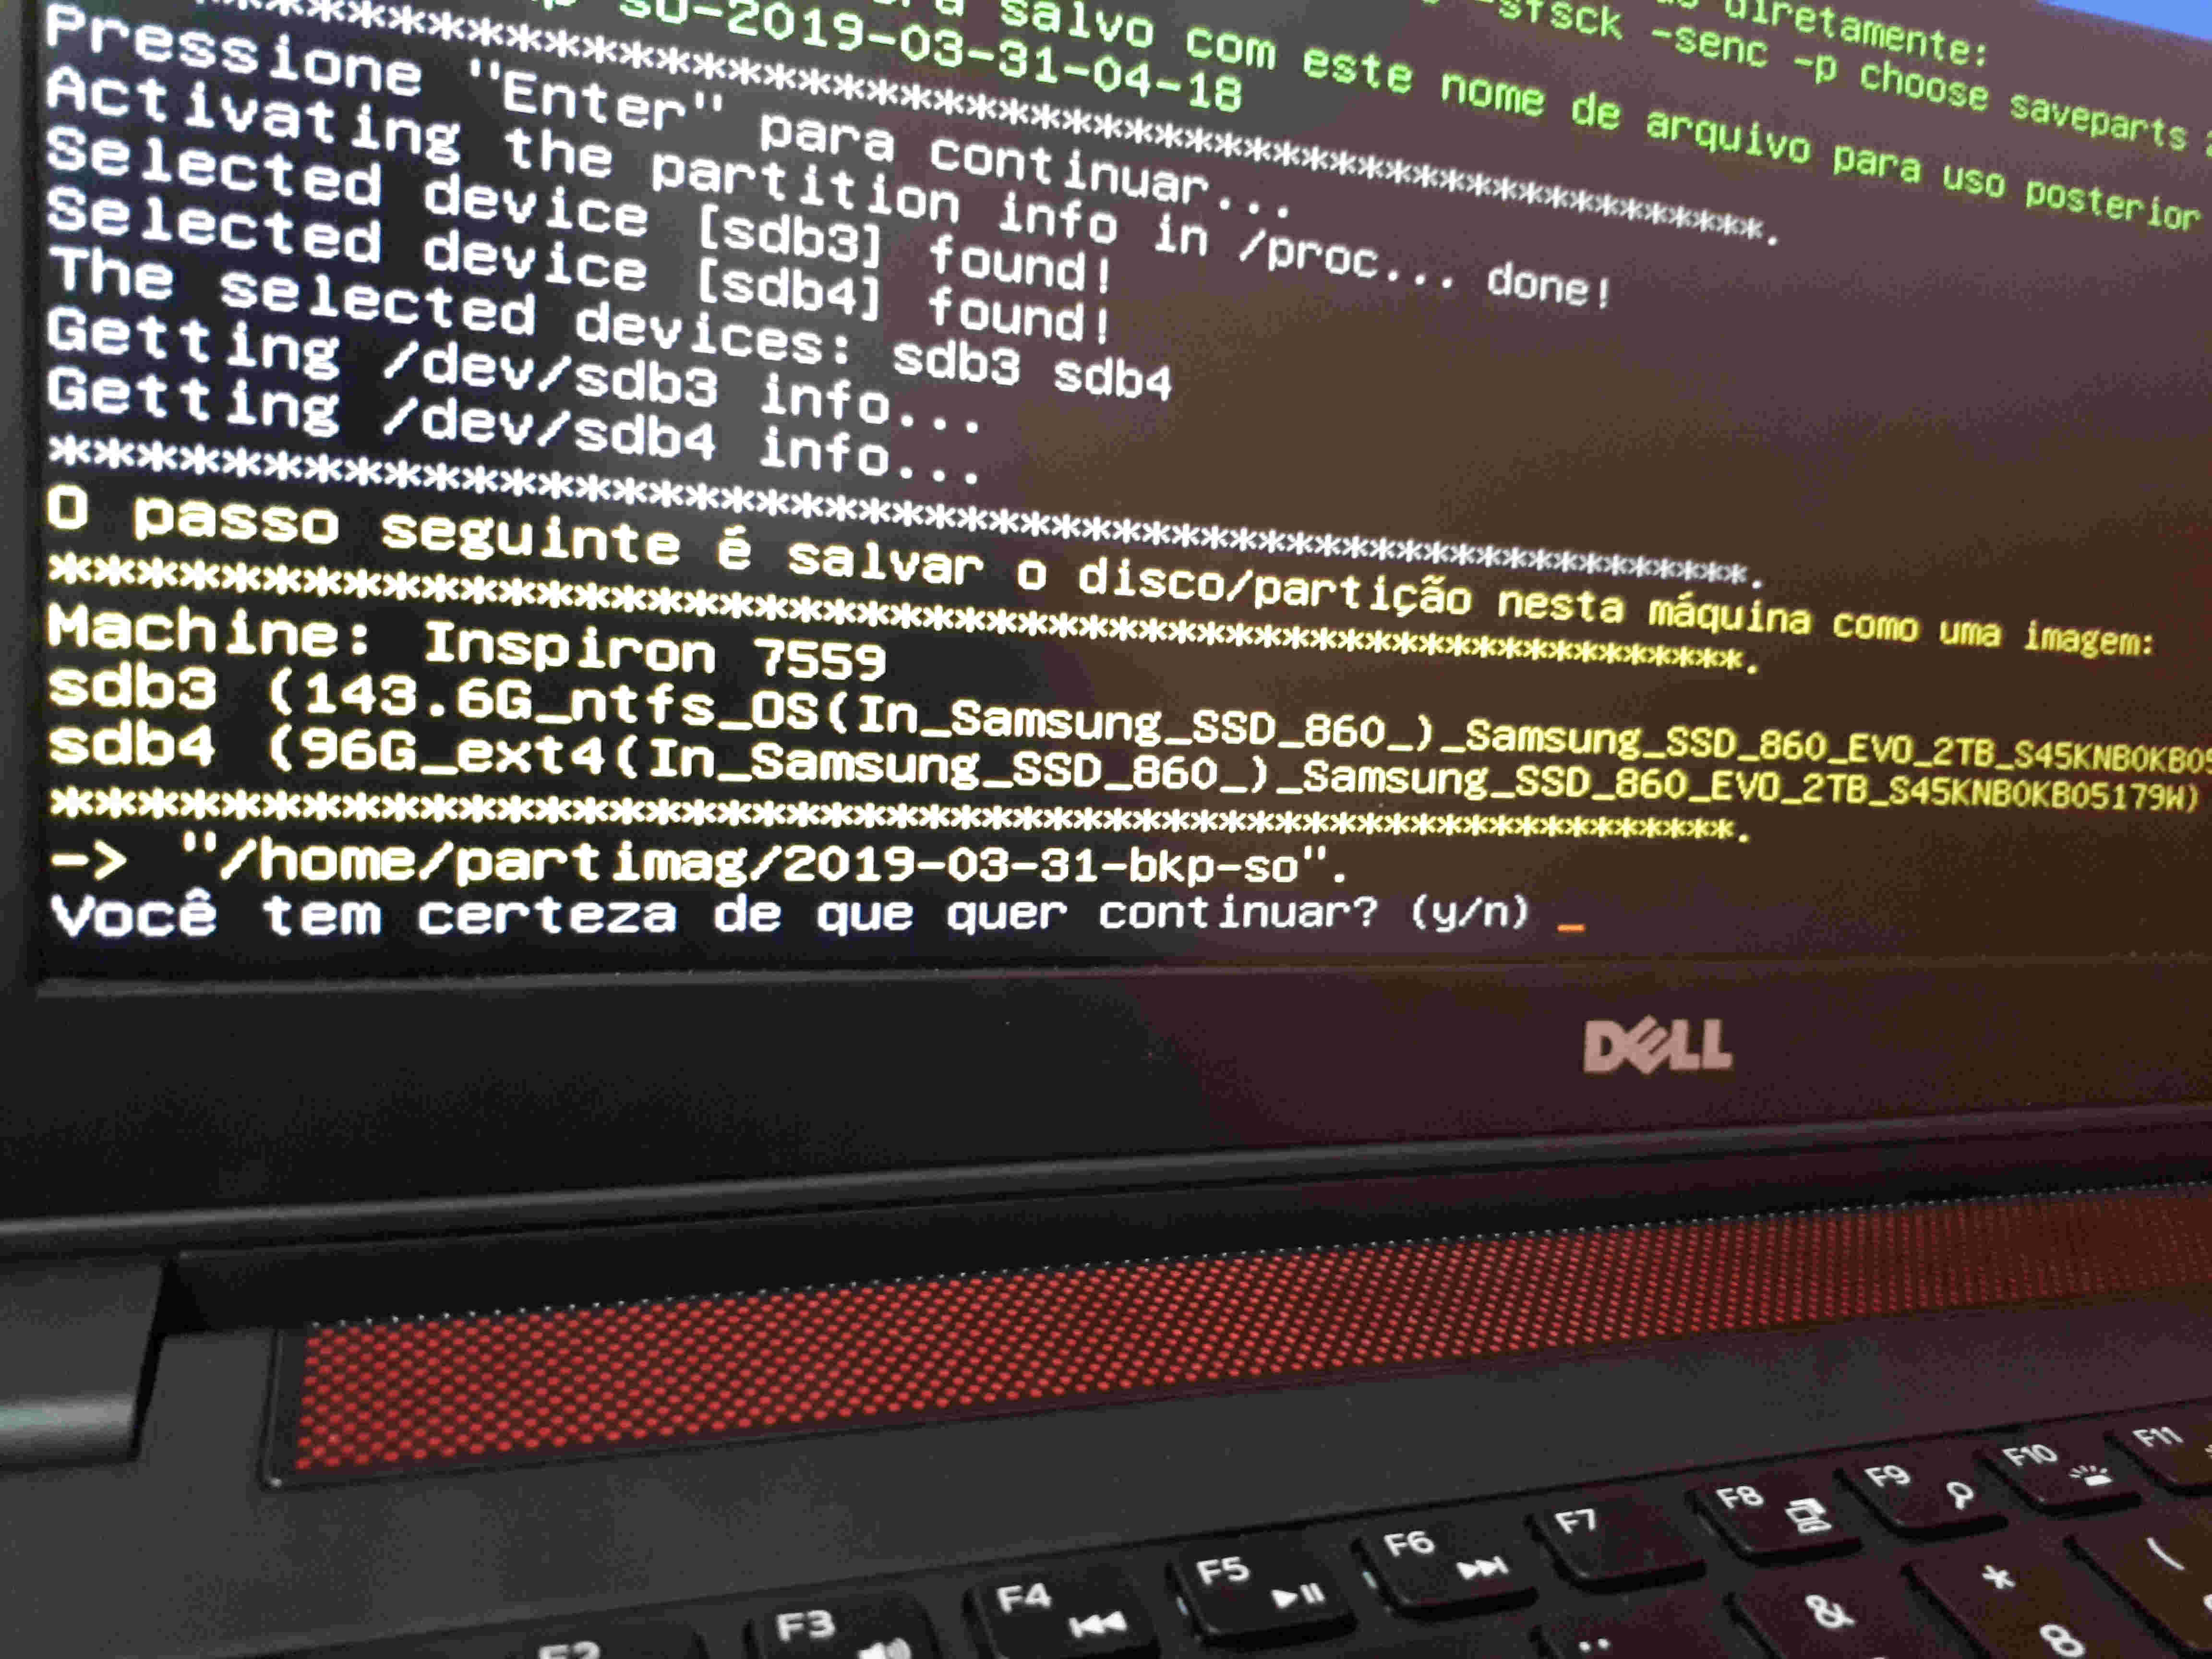
\includegraphics[width=1\linewidth]{images/backup/bkp25.jpg}
        \caption{Partições no Linux Programa GParted}
    \end{figure}
\end{frame}	


\begin{frame}[plain,c]
   \frametitle{\insertsection}
    \framesubtitle{EXECUTANDO O BACKUP}
    \begin{figure}[!h]
        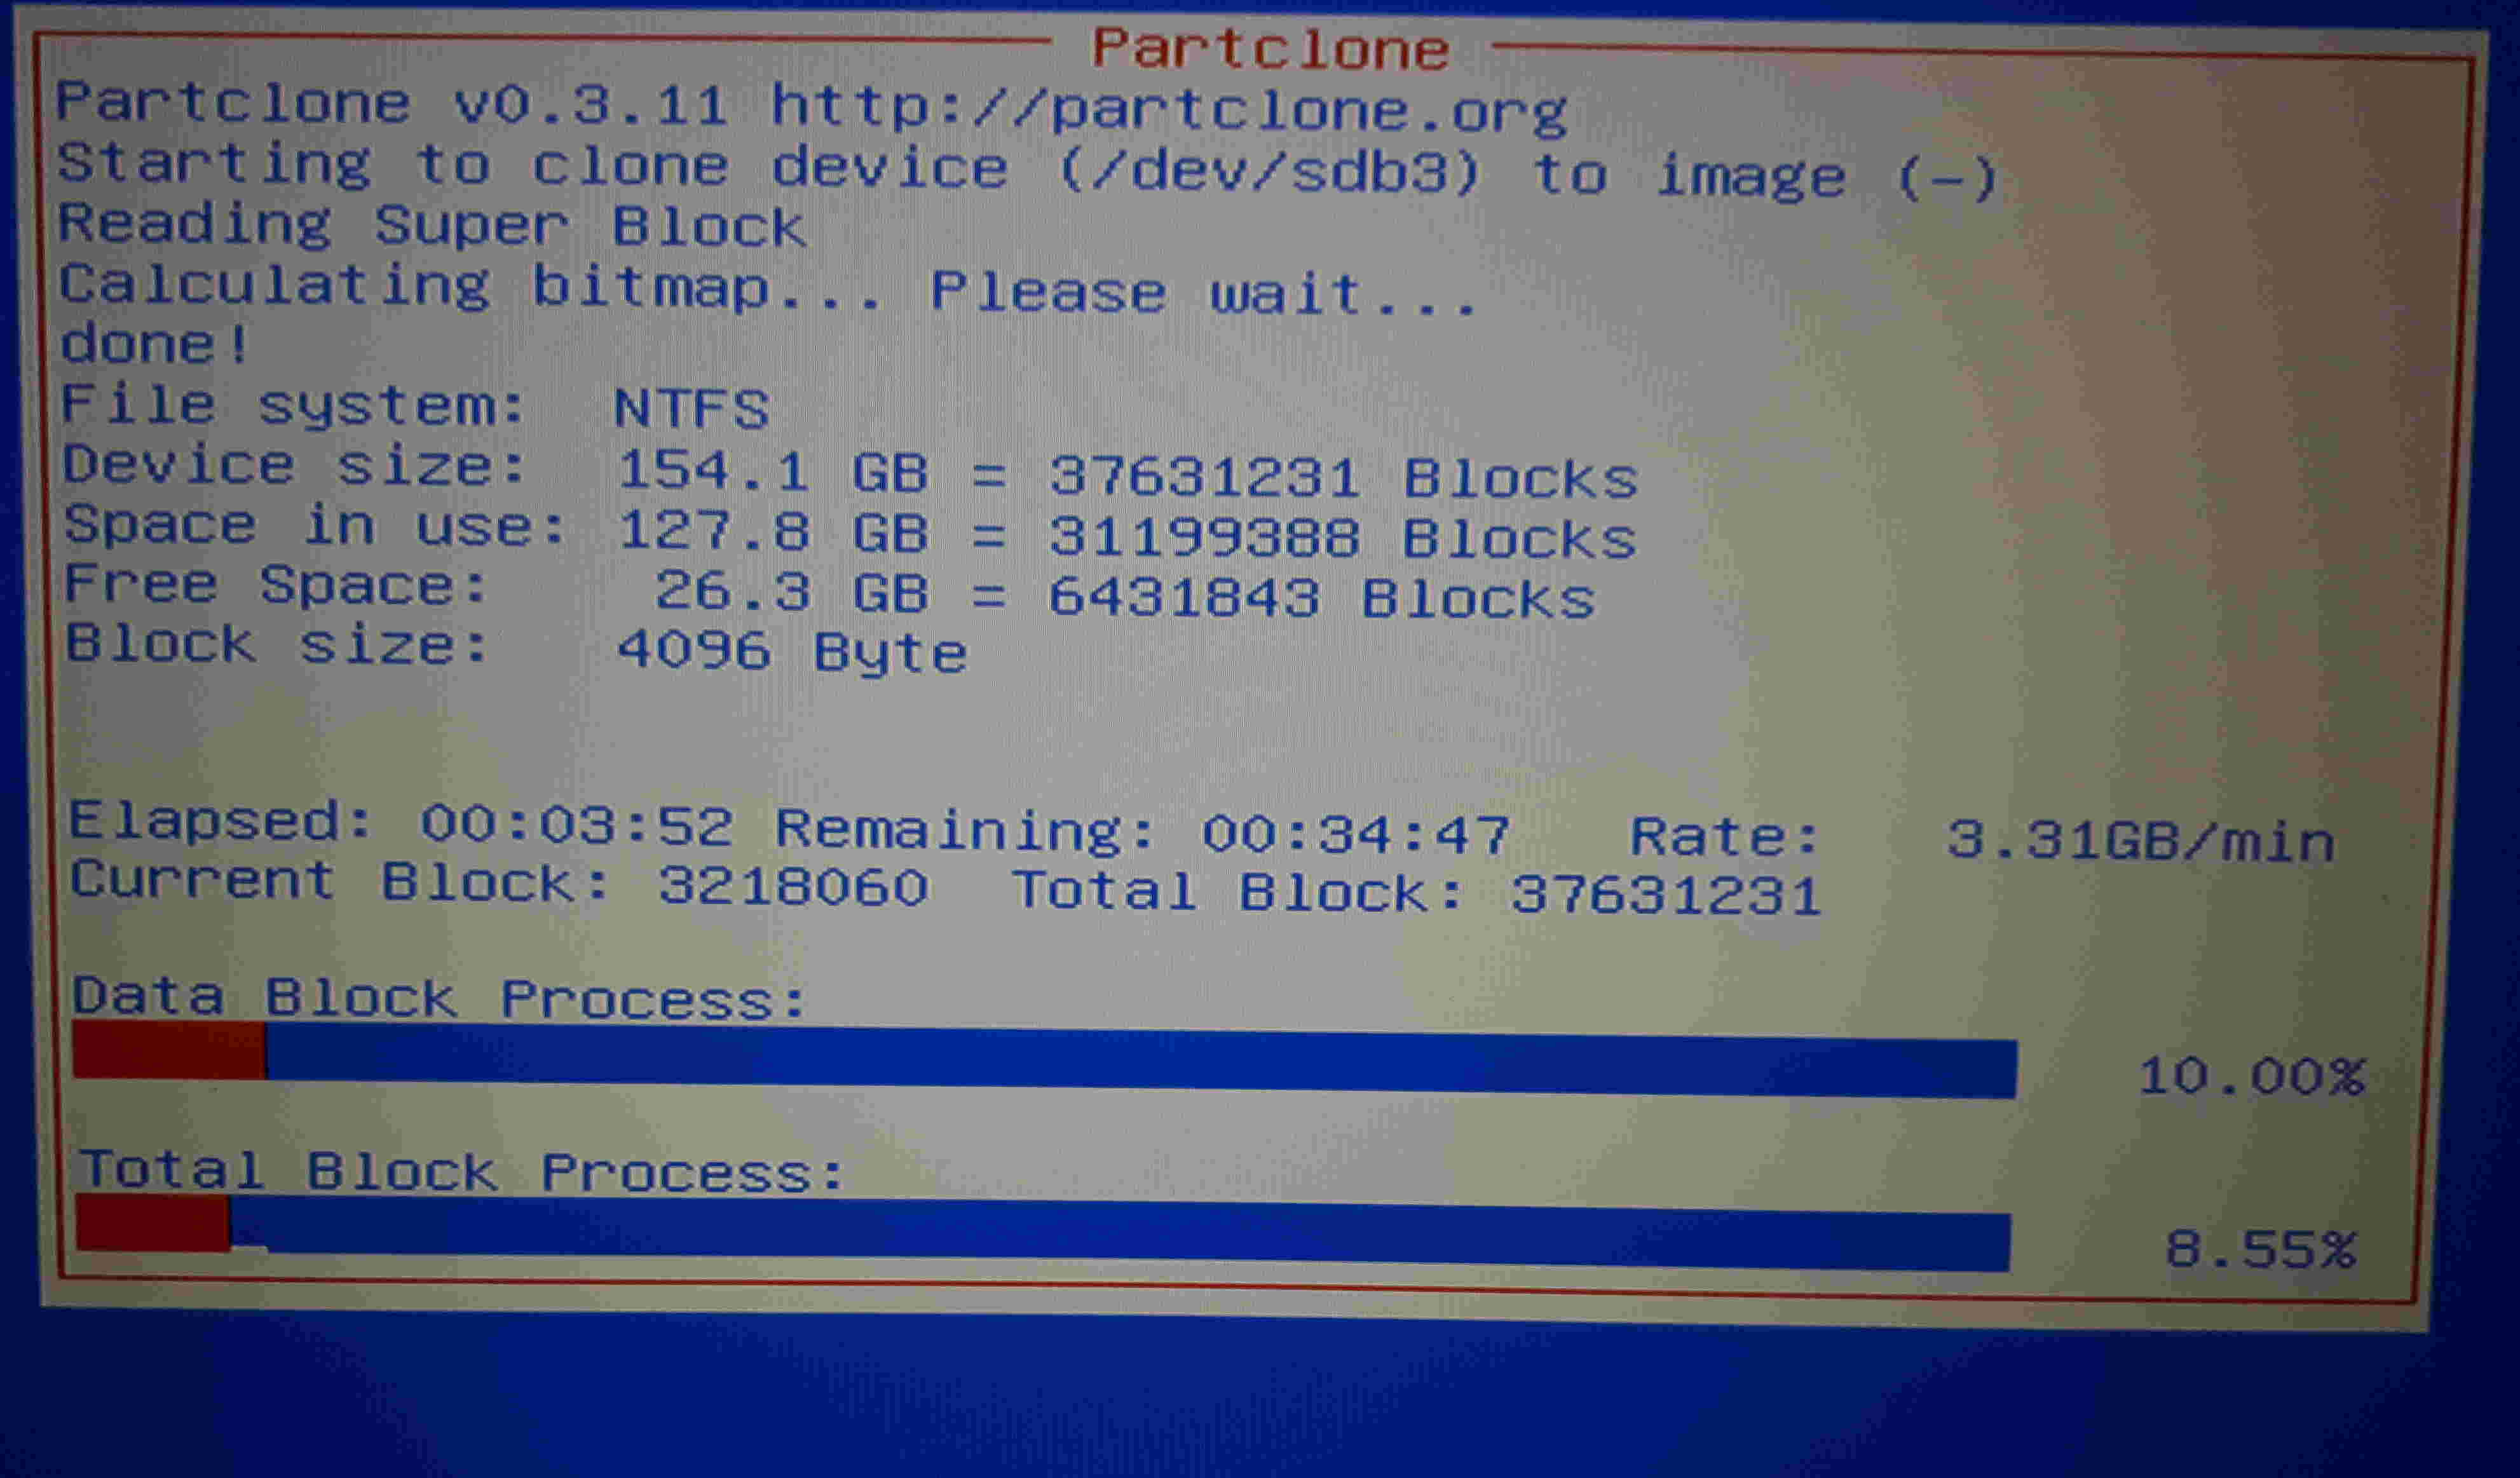
\includegraphics[width=1.1\linewidth]{images/backup/bkp26.jpg}
    \end{figure}
\end{frame}

\begin{frame}[plain,c]
   \frametitle{\insertsection}
    \framesubtitle{EXECUTANDO O BACKUP}
    \begin{figure}[!h]
        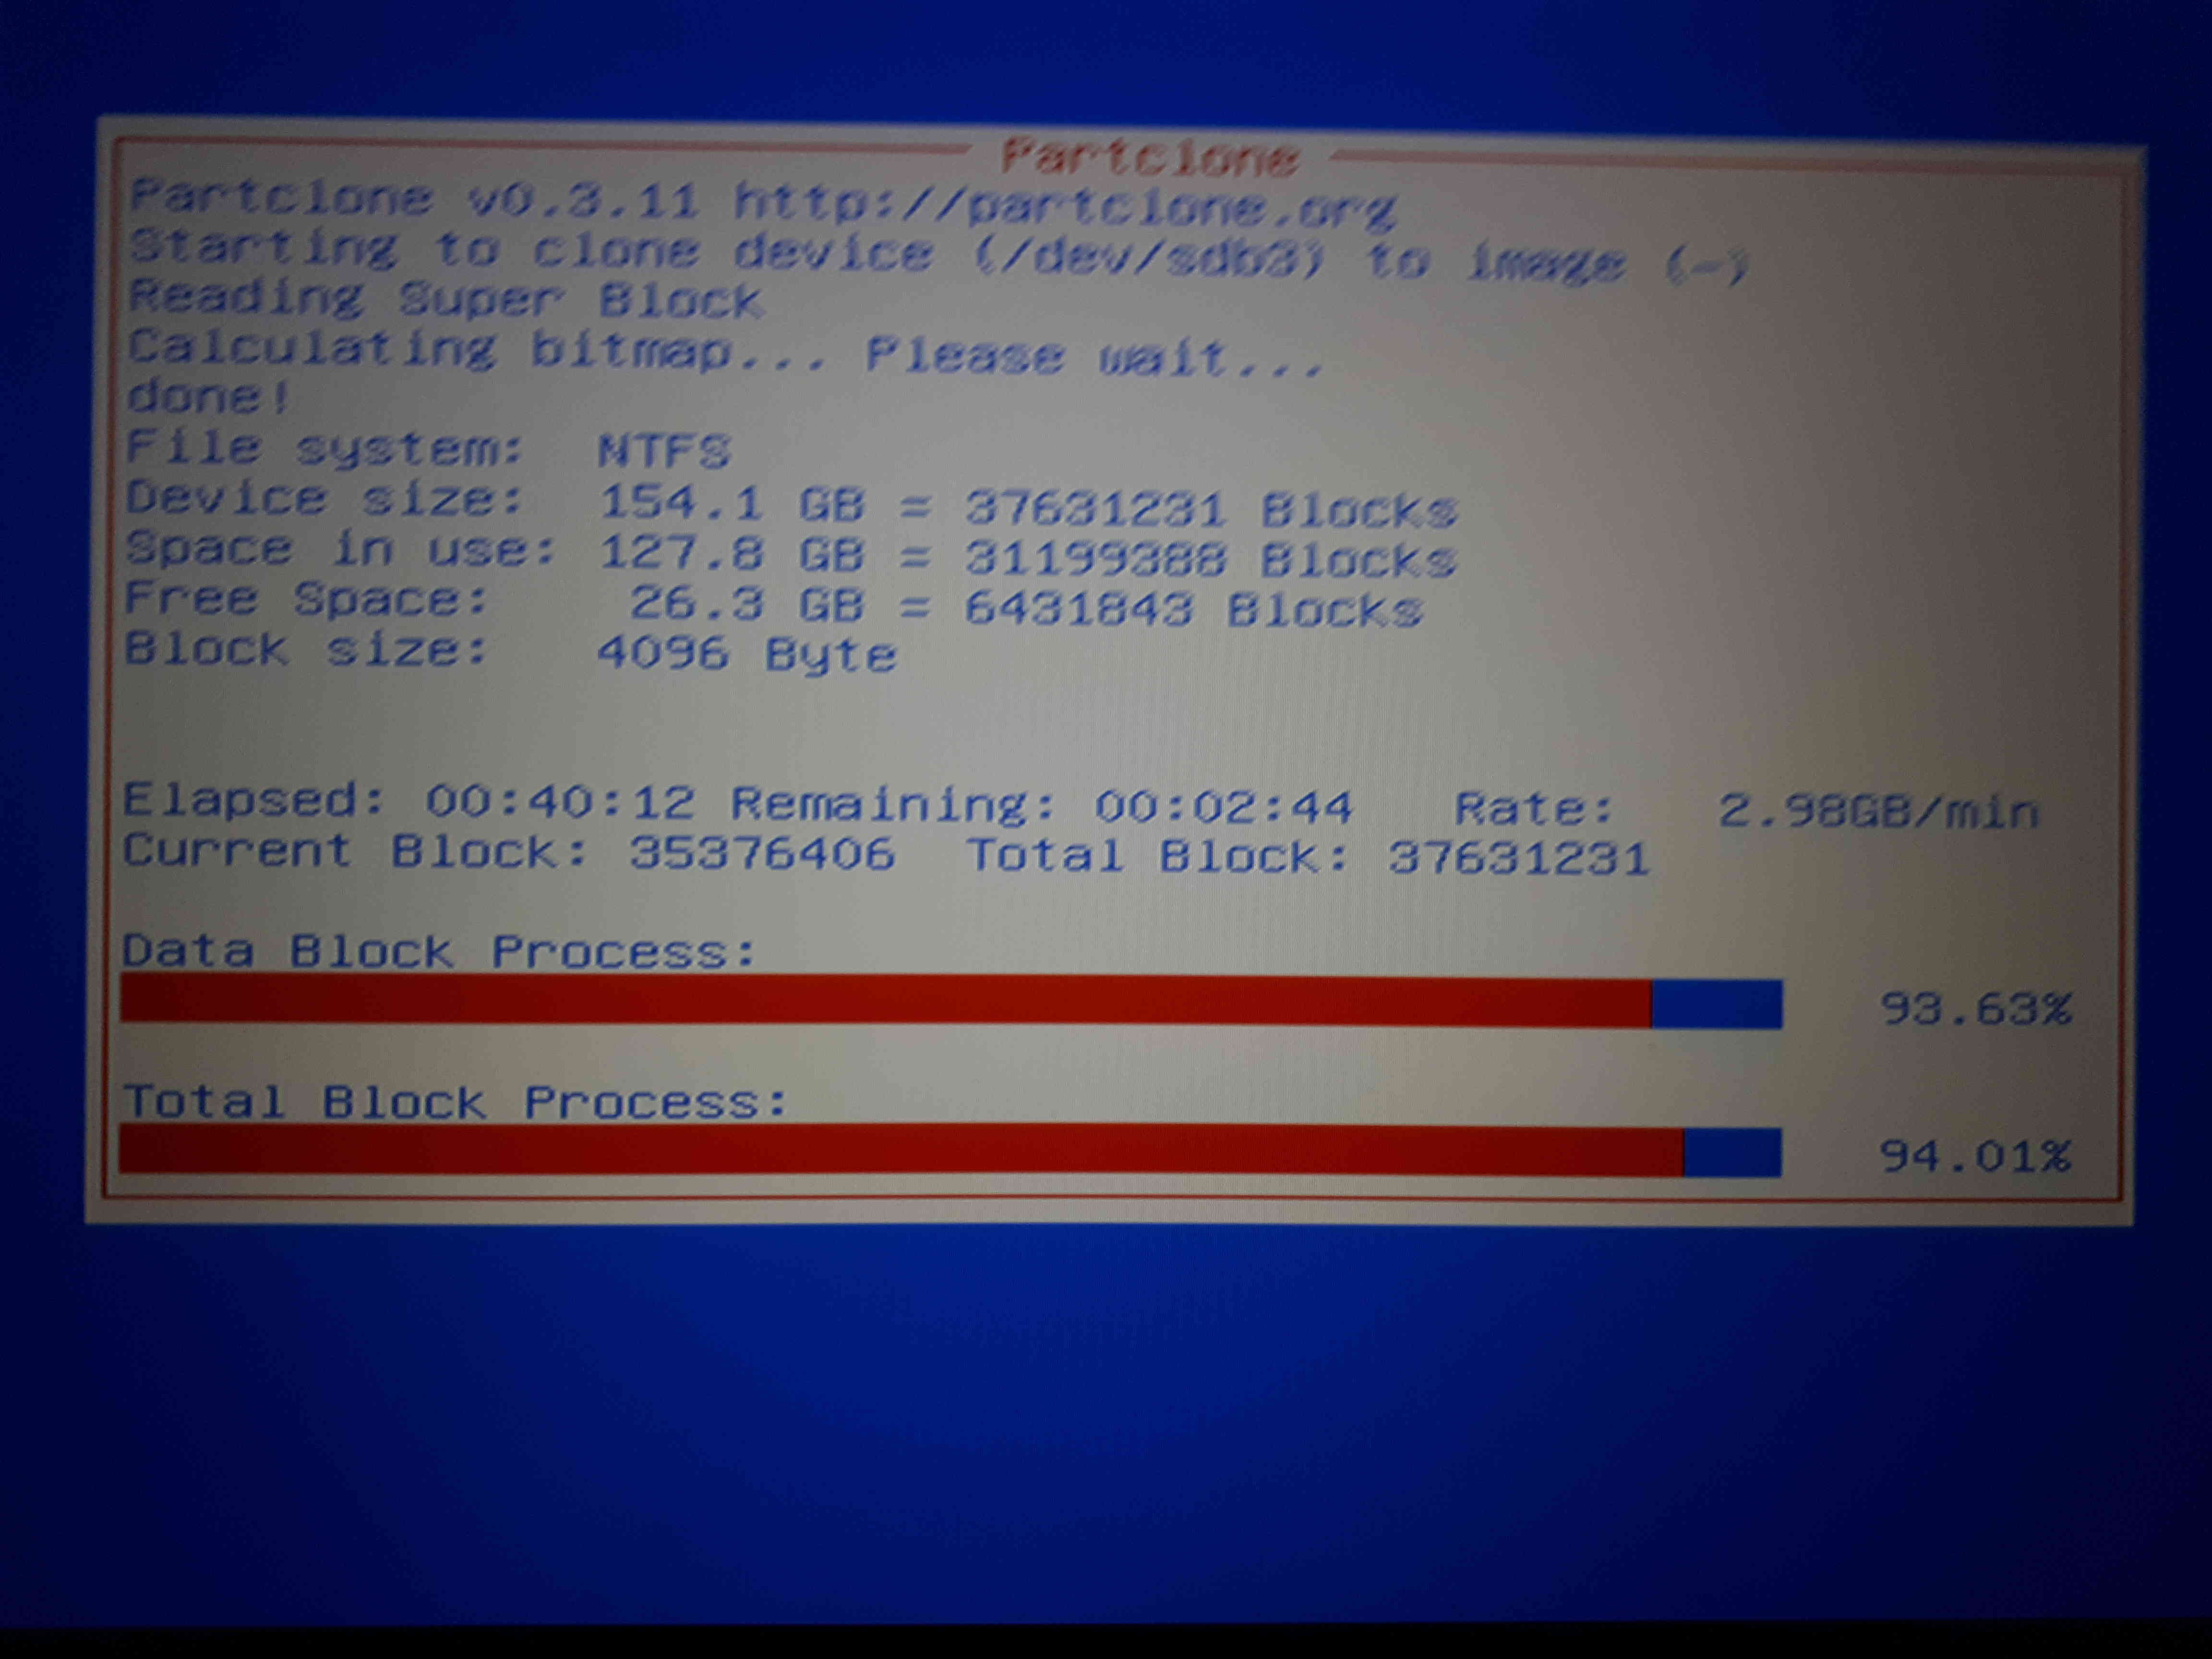
\includegraphics[width=1\linewidth]{images/backup/bkp27.jpg}
        \caption{Partições no Linux Programa GParted}
    \end{figure}
\end{frame}	

\begin{frame}[plain,c]
   \frametitle{\insertsection}
    \framesubtitle{EXECUTANDO O BACKUP}
    \begin{figure}[!h]
        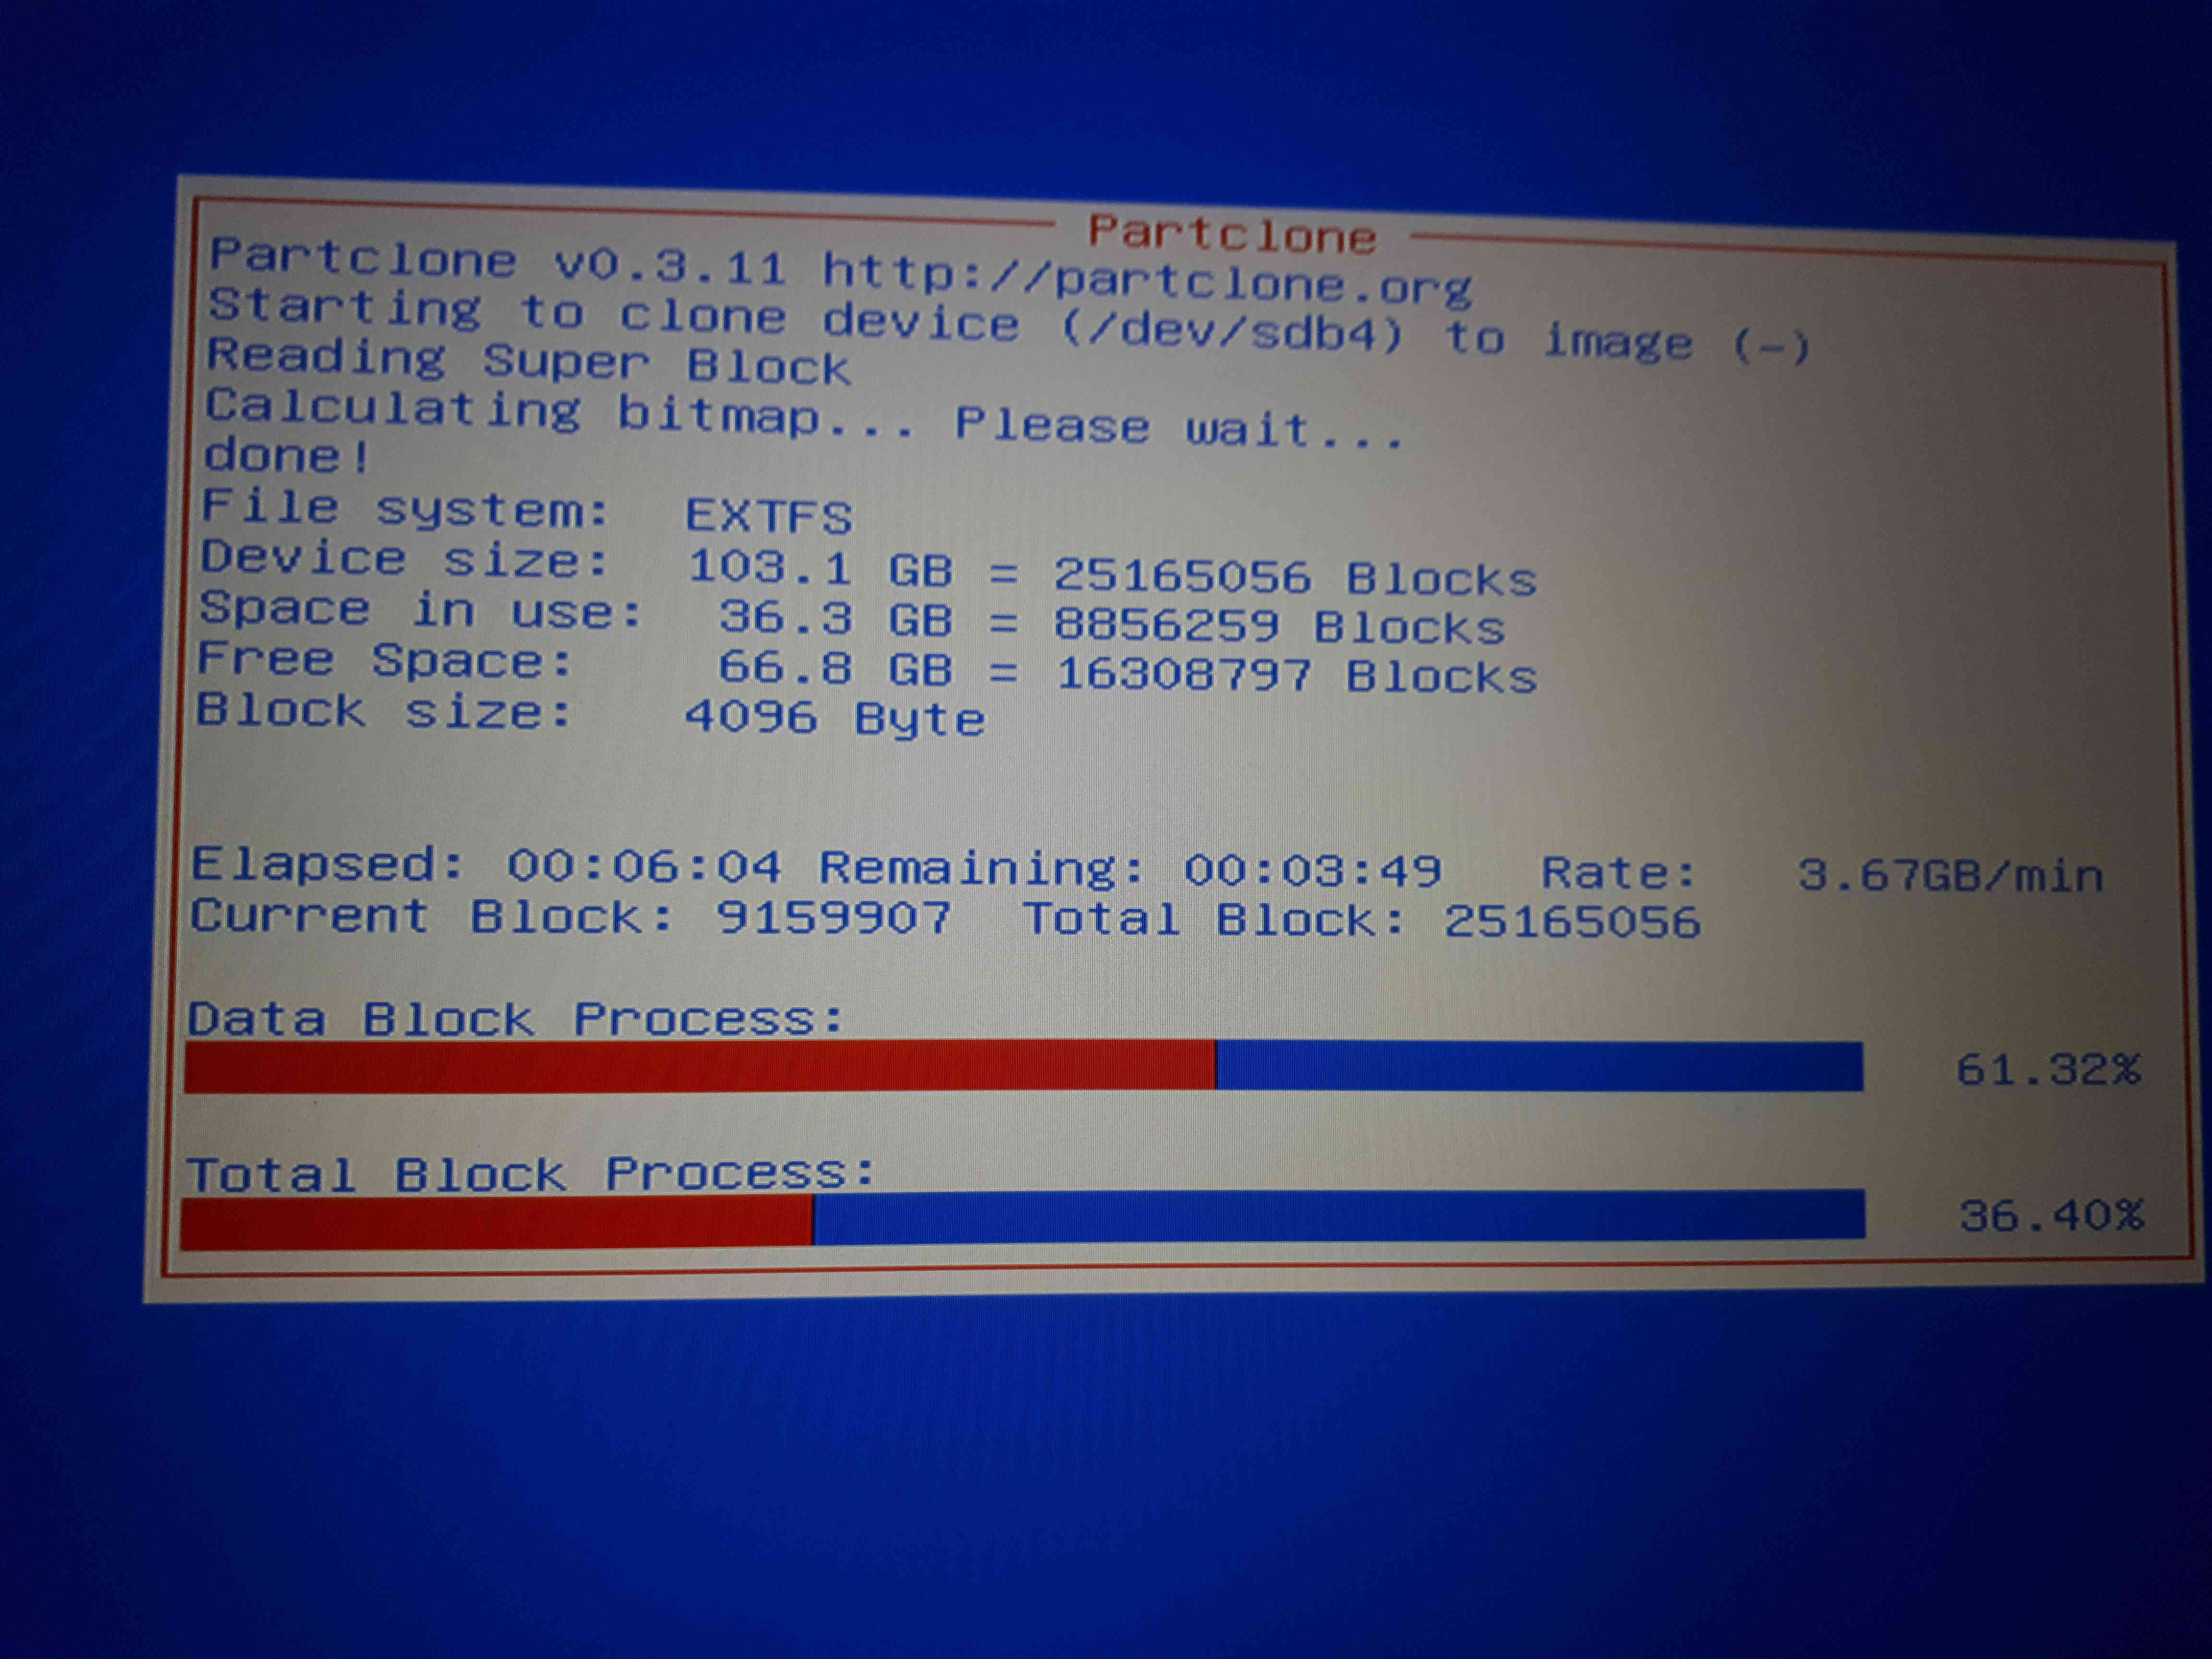
\includegraphics[width=1\linewidth]{images/backup/bkp28.jpg}
        \caption{Partições no Linux Programa GParted}
    \end{figure}
\end{frame}	


\begin{frame}[plain,c]
   \frametitle{\insertsection}
    \framesubtitle{EXECUTANDO O CHEK IMAGE}
    \begin{figure}[!h]
        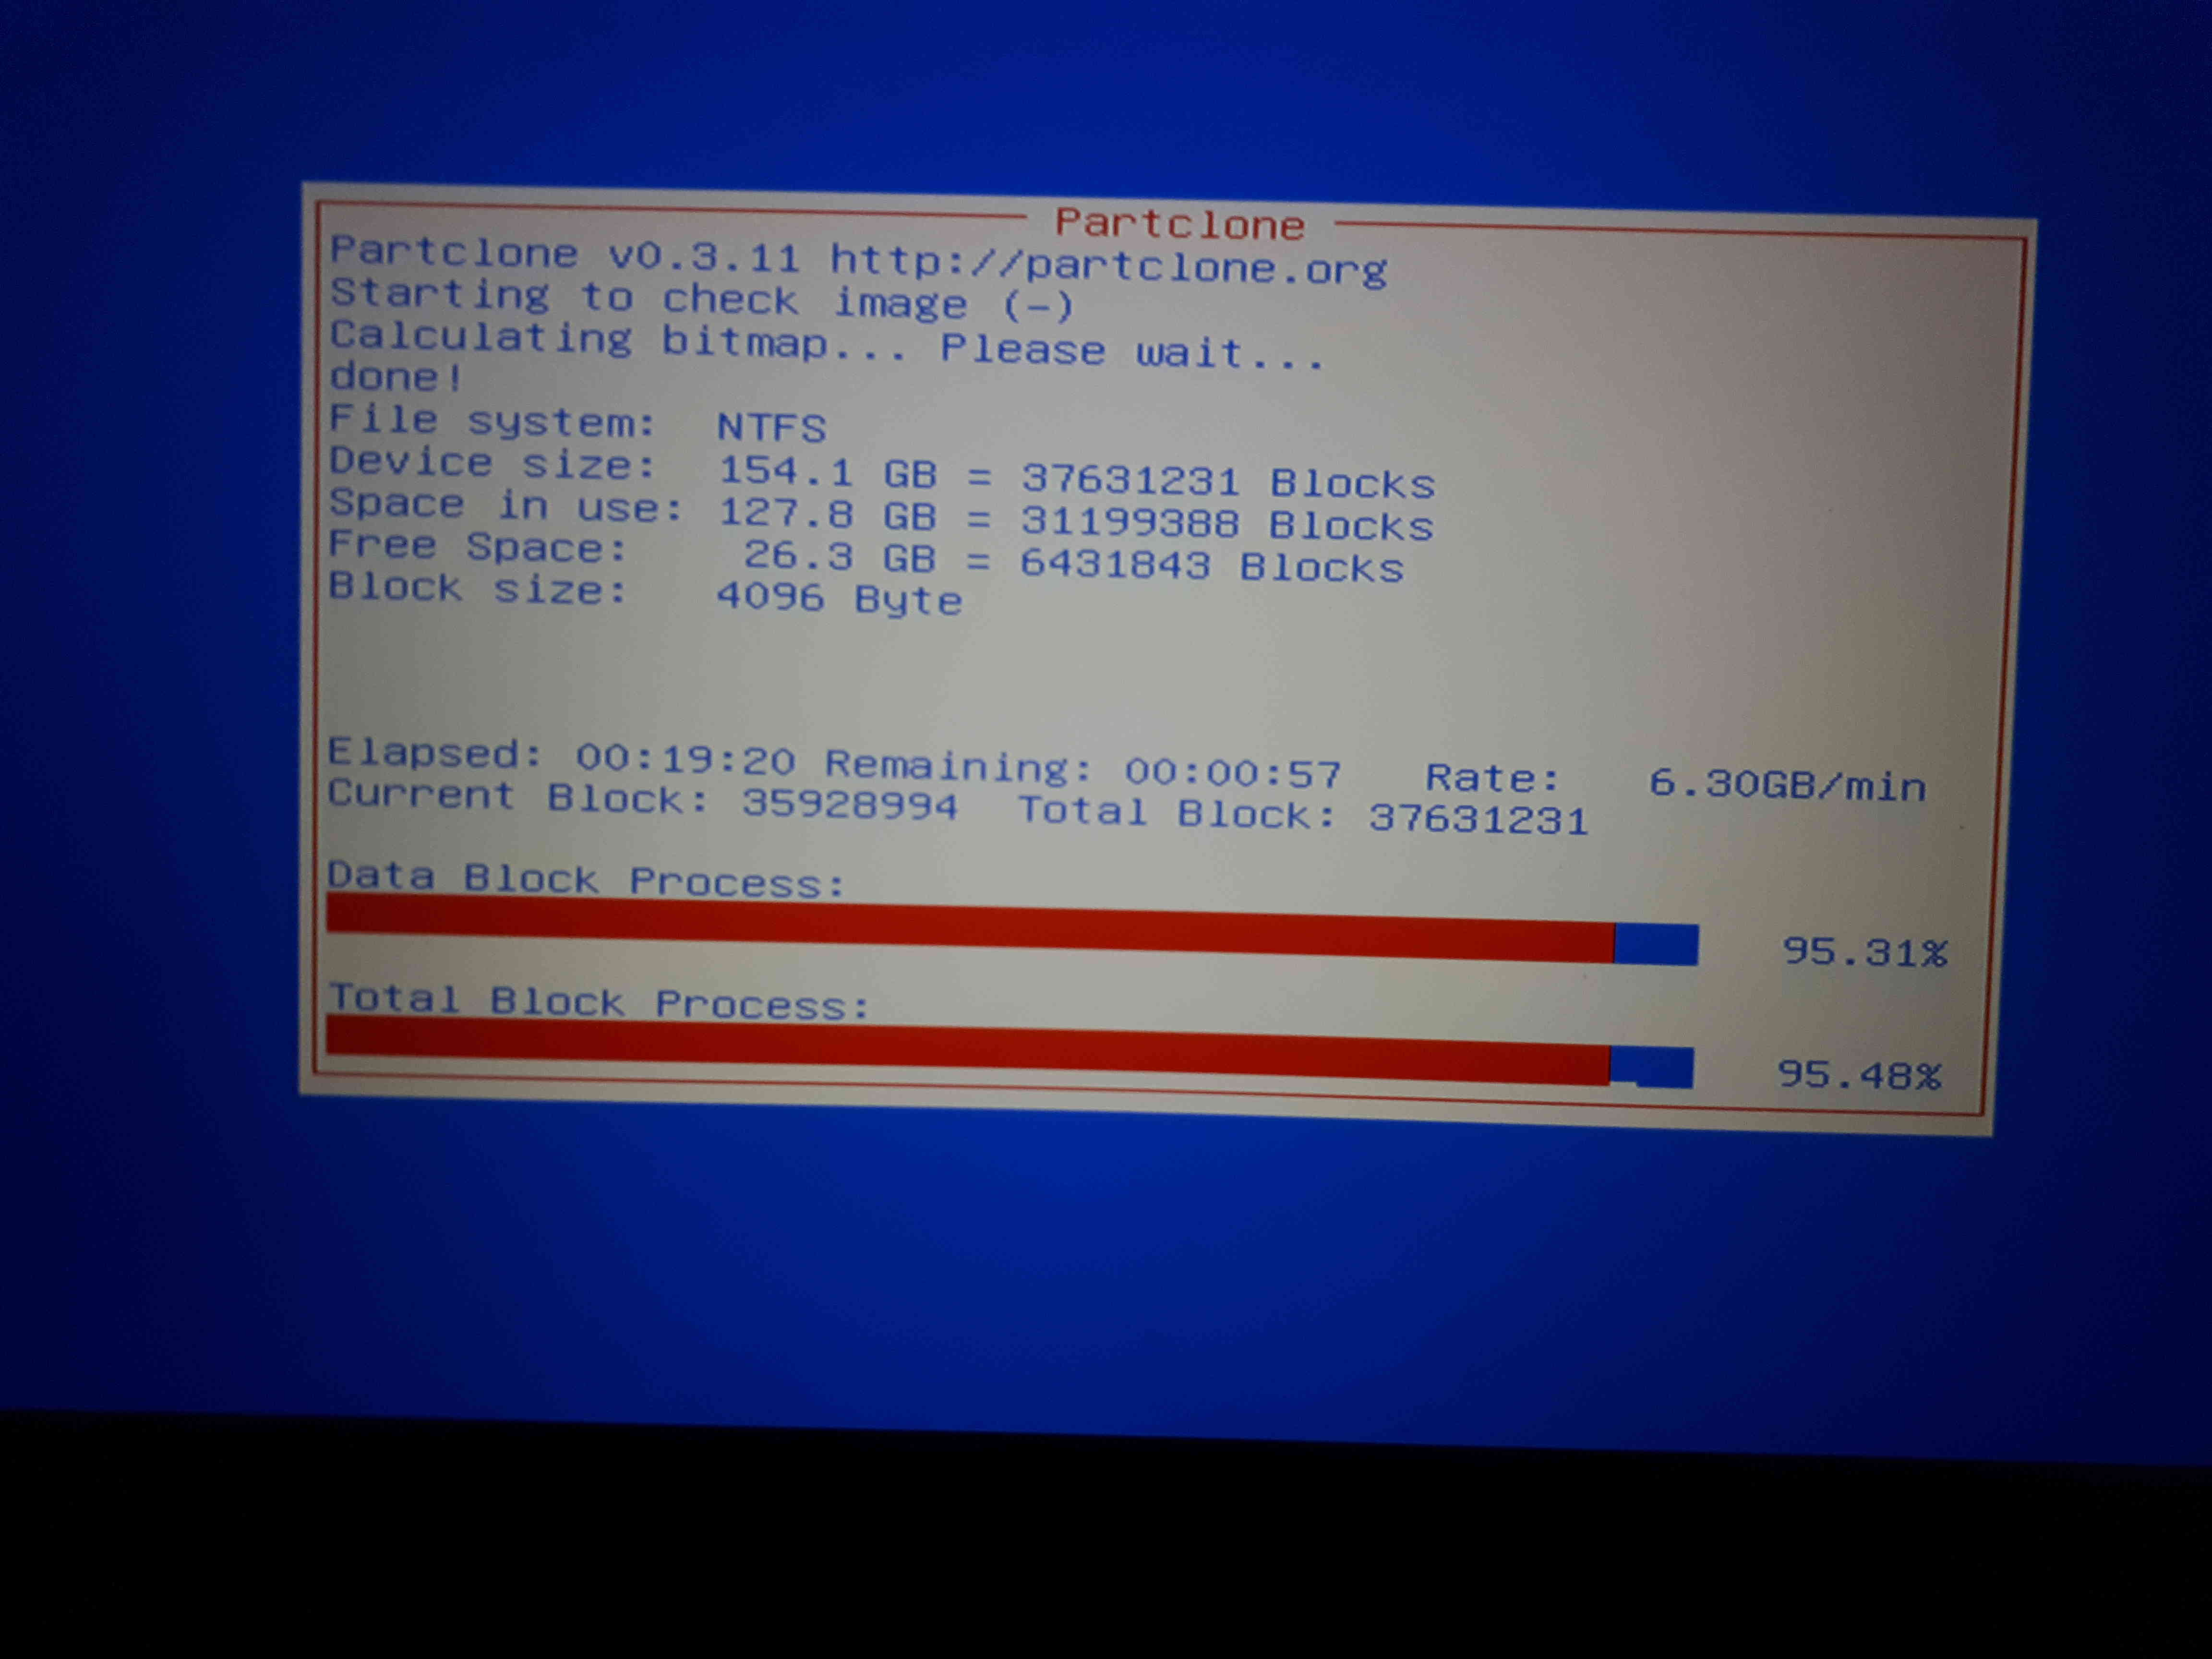
\includegraphics[width=1\linewidth]{images/backup/bkp29.jpg}
        \caption{Partições no Linux Programa GParted}
    \end{figure}
\end{frame}	


\begin{frame}[plain,c]
   \frametitle{\insertsection}
    \framesubtitle{EXECUTANDO O CHEK IMAGE}
    \begin{figure}[!h]
        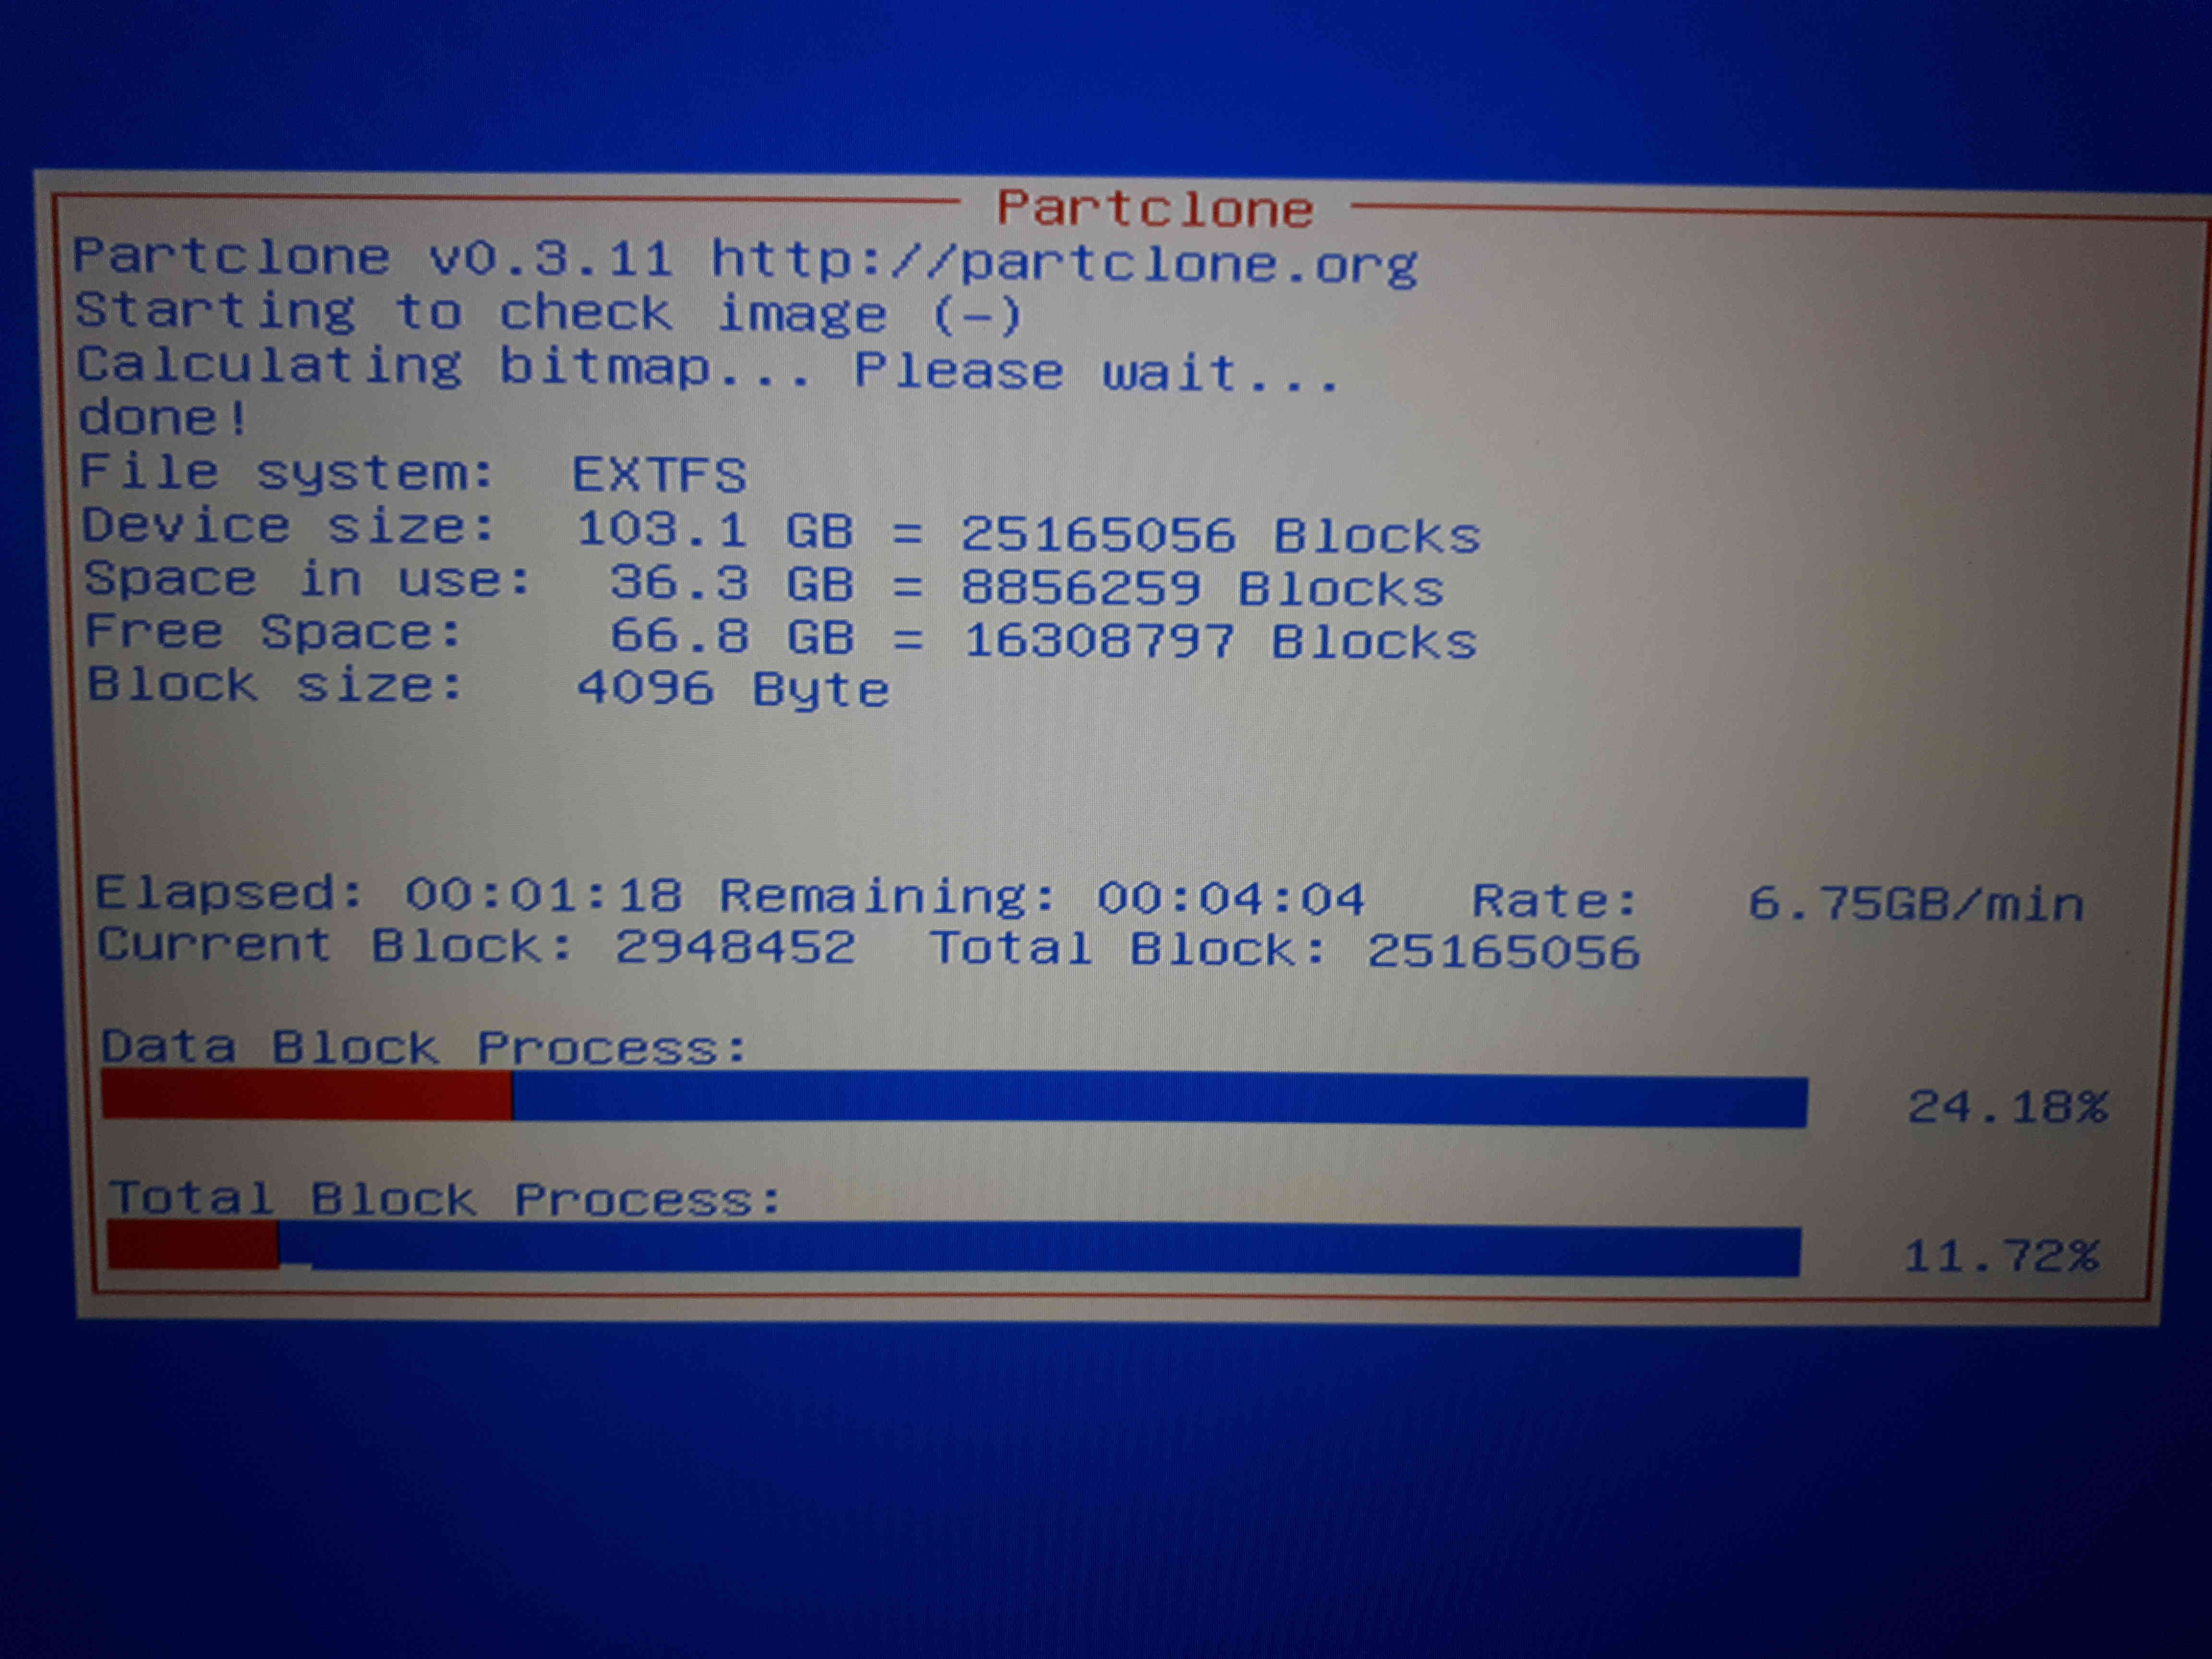
\includegraphics[width=1\linewidth]{images/backup/bkp30.jpg}
        \caption{Partições no Linux Programa GParted}
    \end{figure}
\end{frame}	


\begin{frame}[plain,c]
   \frametitle{\insertsection}
    \framesubtitle{BACKUP FINALIZADO}
    \begin{figure}[!h]
        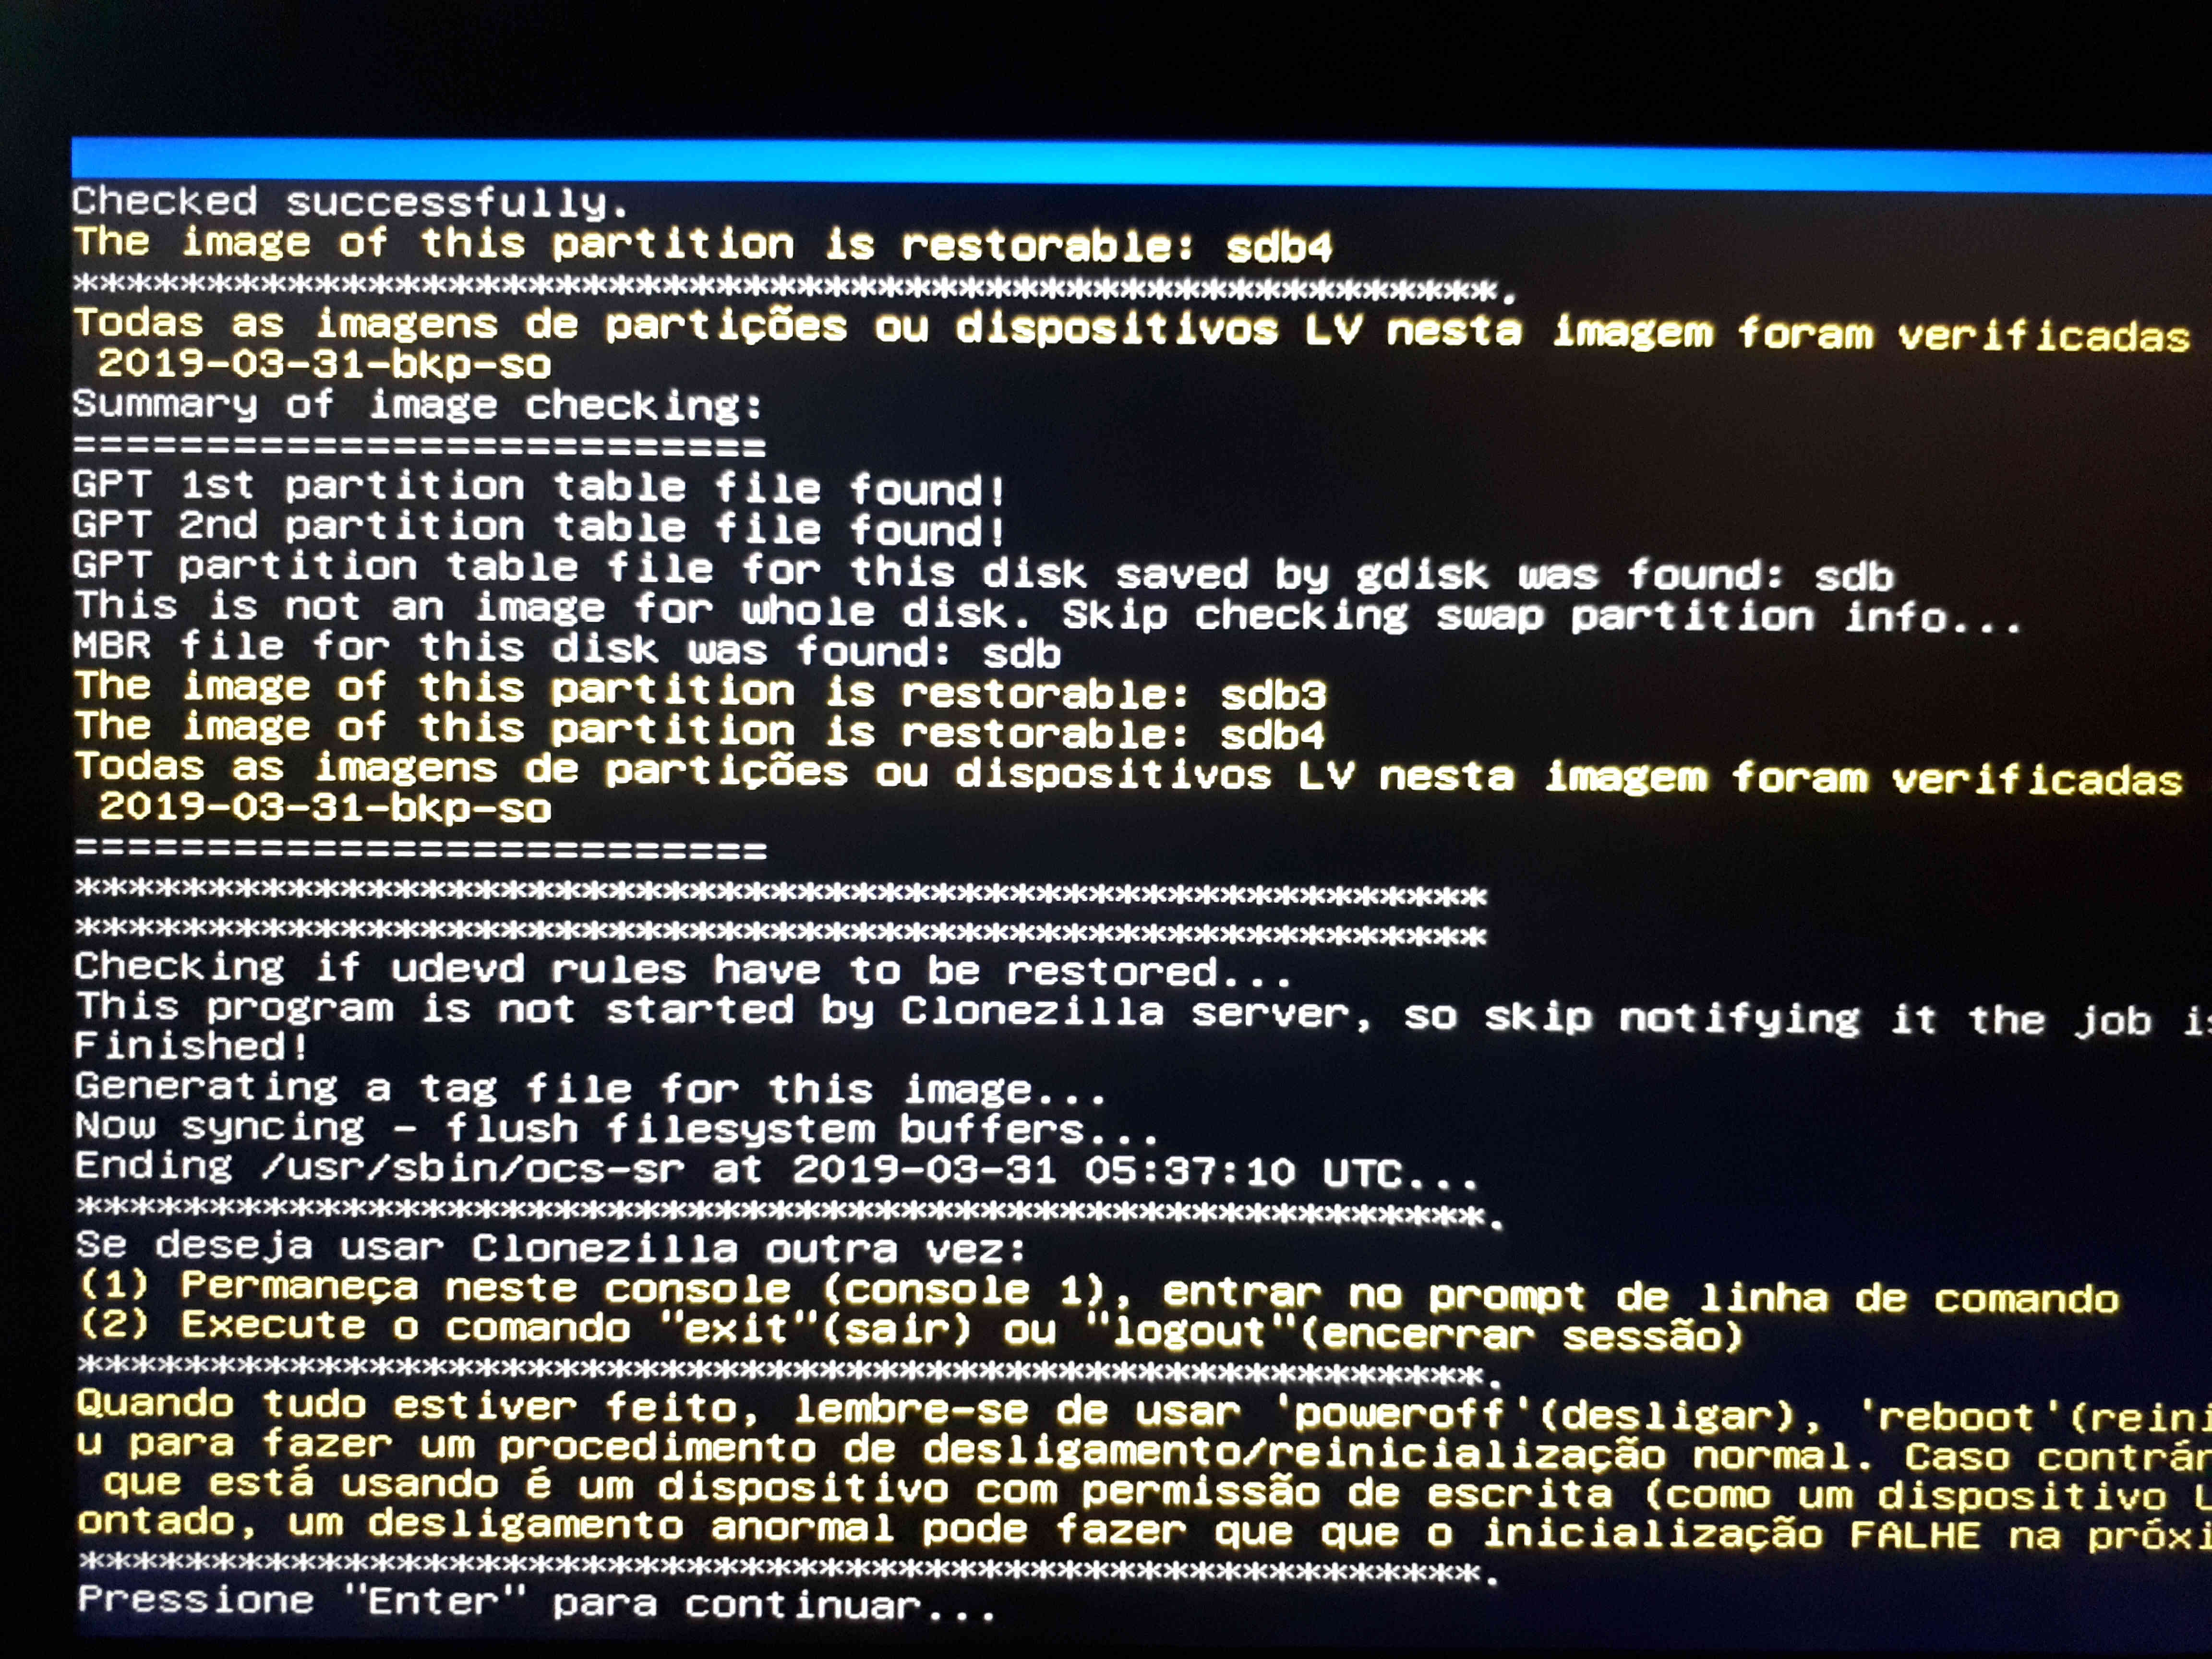
\includegraphics[width=1\linewidth]{images/backup/bkp31.jpg}
        \caption{Partições no Linux Programa GParted}
    \end{figure}
\end{frame}	

\begin{frame}[plain,c]
   \frametitle{\insertsection}
    \framesubtitle{BACKUP FINALIZADO}
    \begin{figure}[!h]
        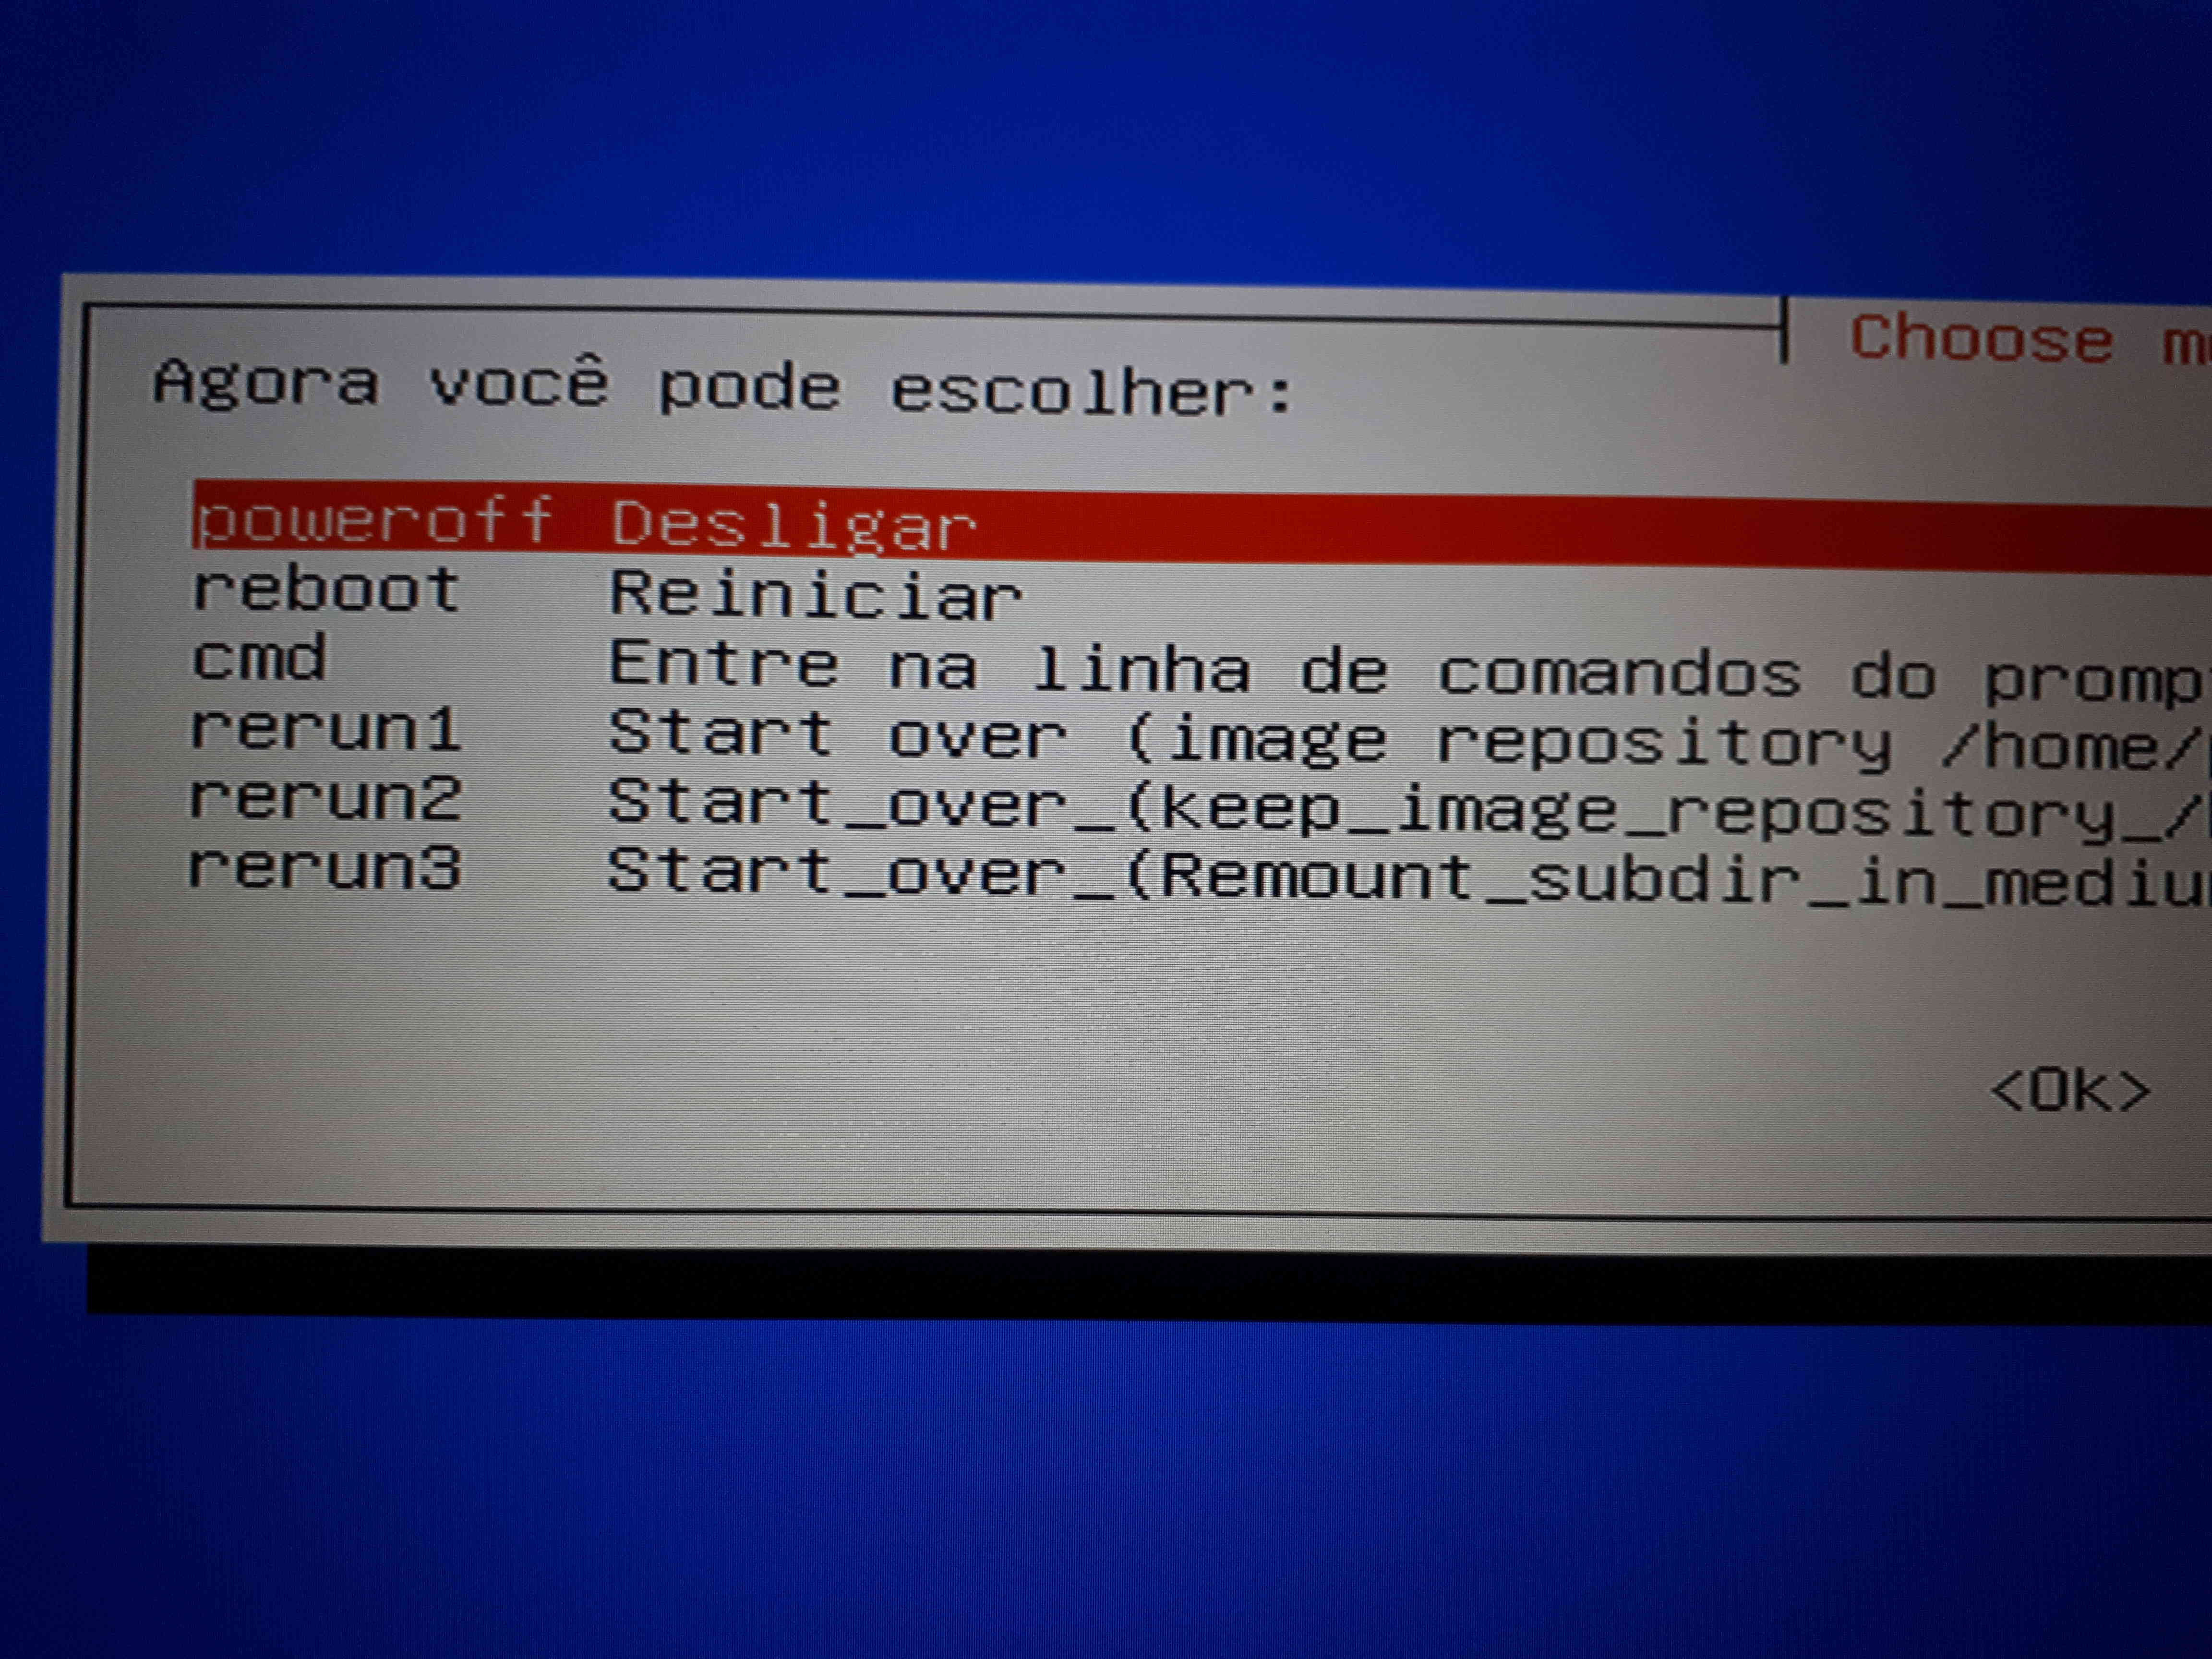
\includegraphics[width=1\linewidth]{images/backup/bkp32.jpg}
        \caption{Partições no Linux Programa GParted}
    \end{figure}
\end{frame}	

\section{Restauração de Partições}
\subsection{Tutorial de Restauração de uma Partição}
\begin{frame}
    \frametitle{\insertsection}
    \framesubtitle{\insertsubsection}
     \begin{block}{\insertsubsection}
  	\justifying
  Para realizar a restauração de uma partição a partir de uma IMAGEM são necessários os seguintes passos:
  
   \begin{itemize}[<+-| alert@+>]
        \item Dar boot do pendrive com o CLONEZILLA .
        \item Inicializar a partir do pendrive (F2,F12,F8,F9, dependendo da BIOS da placa-mãe).
        \item Saber identificar a partição de origem (SDA1, SDB1 etc...).
        \item Ter acesso ao HD ou partição onde foi salvo o arquivo de IMAGEM.
  		\item ATENÇÃO: A RESTAURAÇÃO APAGA TODOS OS ARQUIVOS EXISTENTES NA PARTIÇÃO, VOLTANDO AO ESTADO ANTERIOR Á CRIAÇÃO DA IMAGEM.
	  \end{itemize}
\end{block}
\end{frame}

\begin{frame}[plain,c]
   \frametitle{\insertsection}
    \framesubtitle{Inicializando pelo pendrive}
    \begin{figure}[!h]
        
        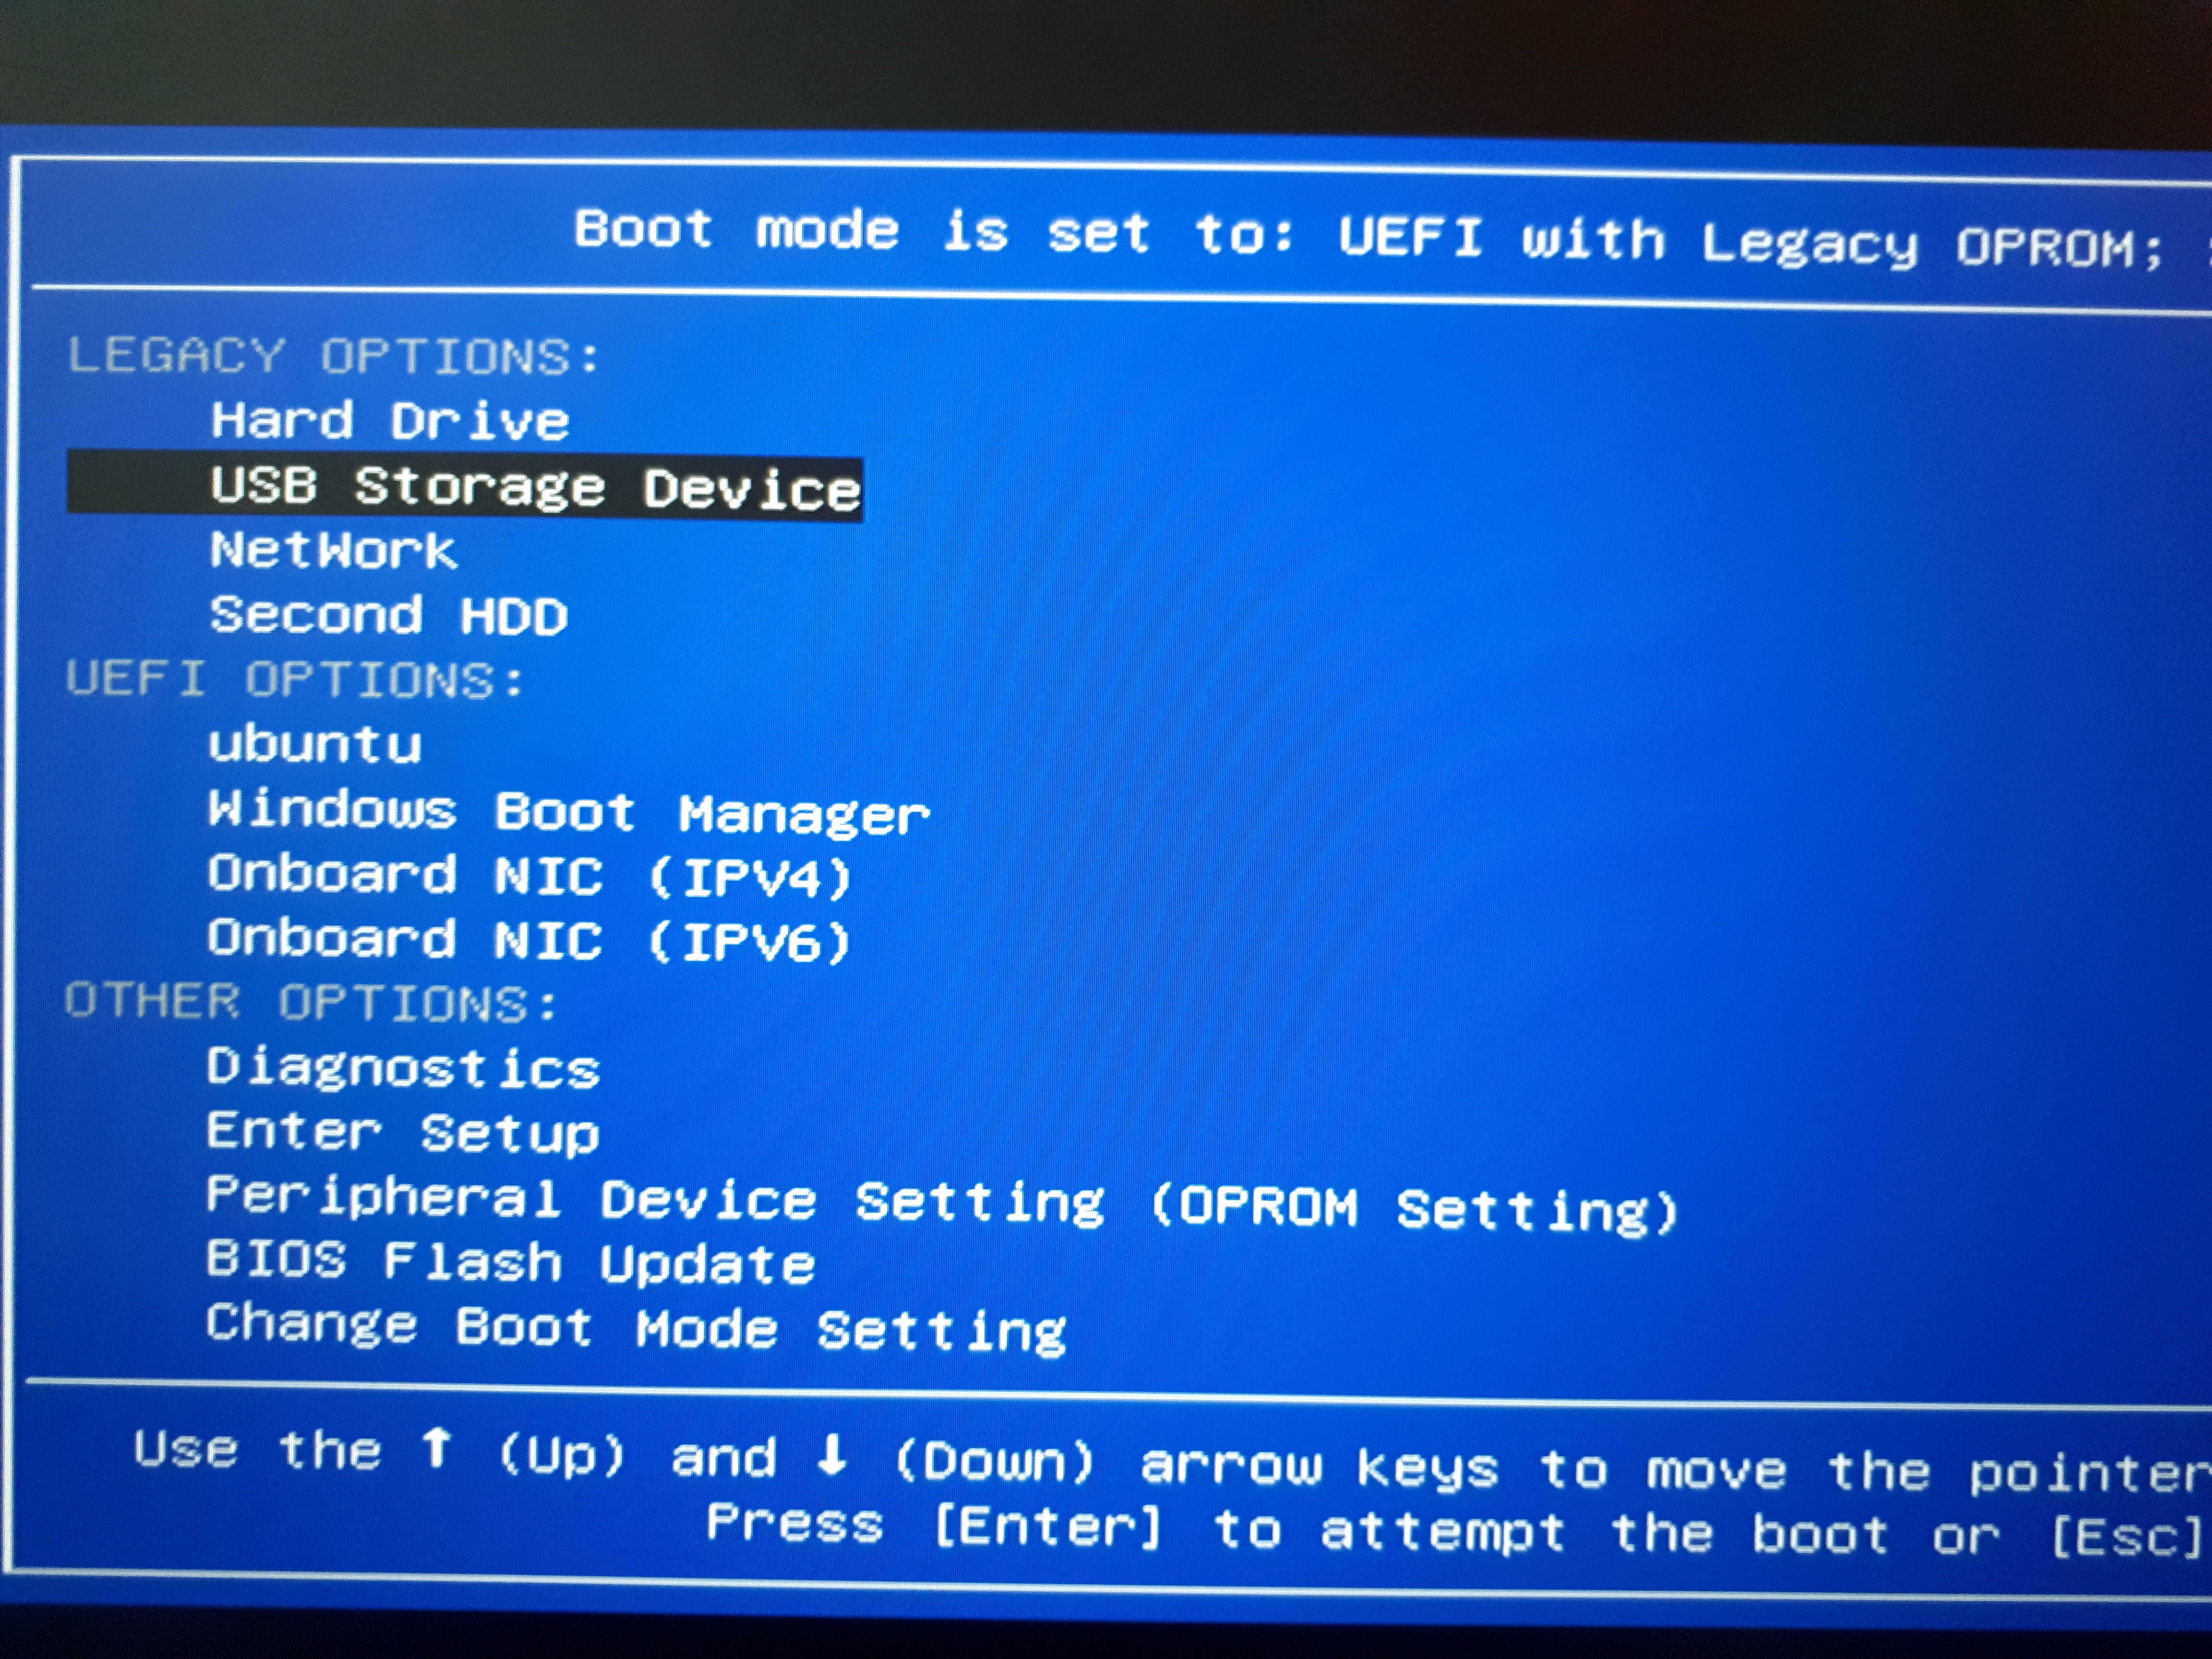
\includegraphics[width=1\linewidth]{images/backup/bkp1.jpg}
        \caption{Partições no Linux Programa GParted}
    \end{figure}
\end{frame}

\begin{frame}[plain,c]
   \frametitle{\insertsection}
    \framesubtitle{Tela inicial do CloneZilla}
    \begin{figure}[!h]
        
        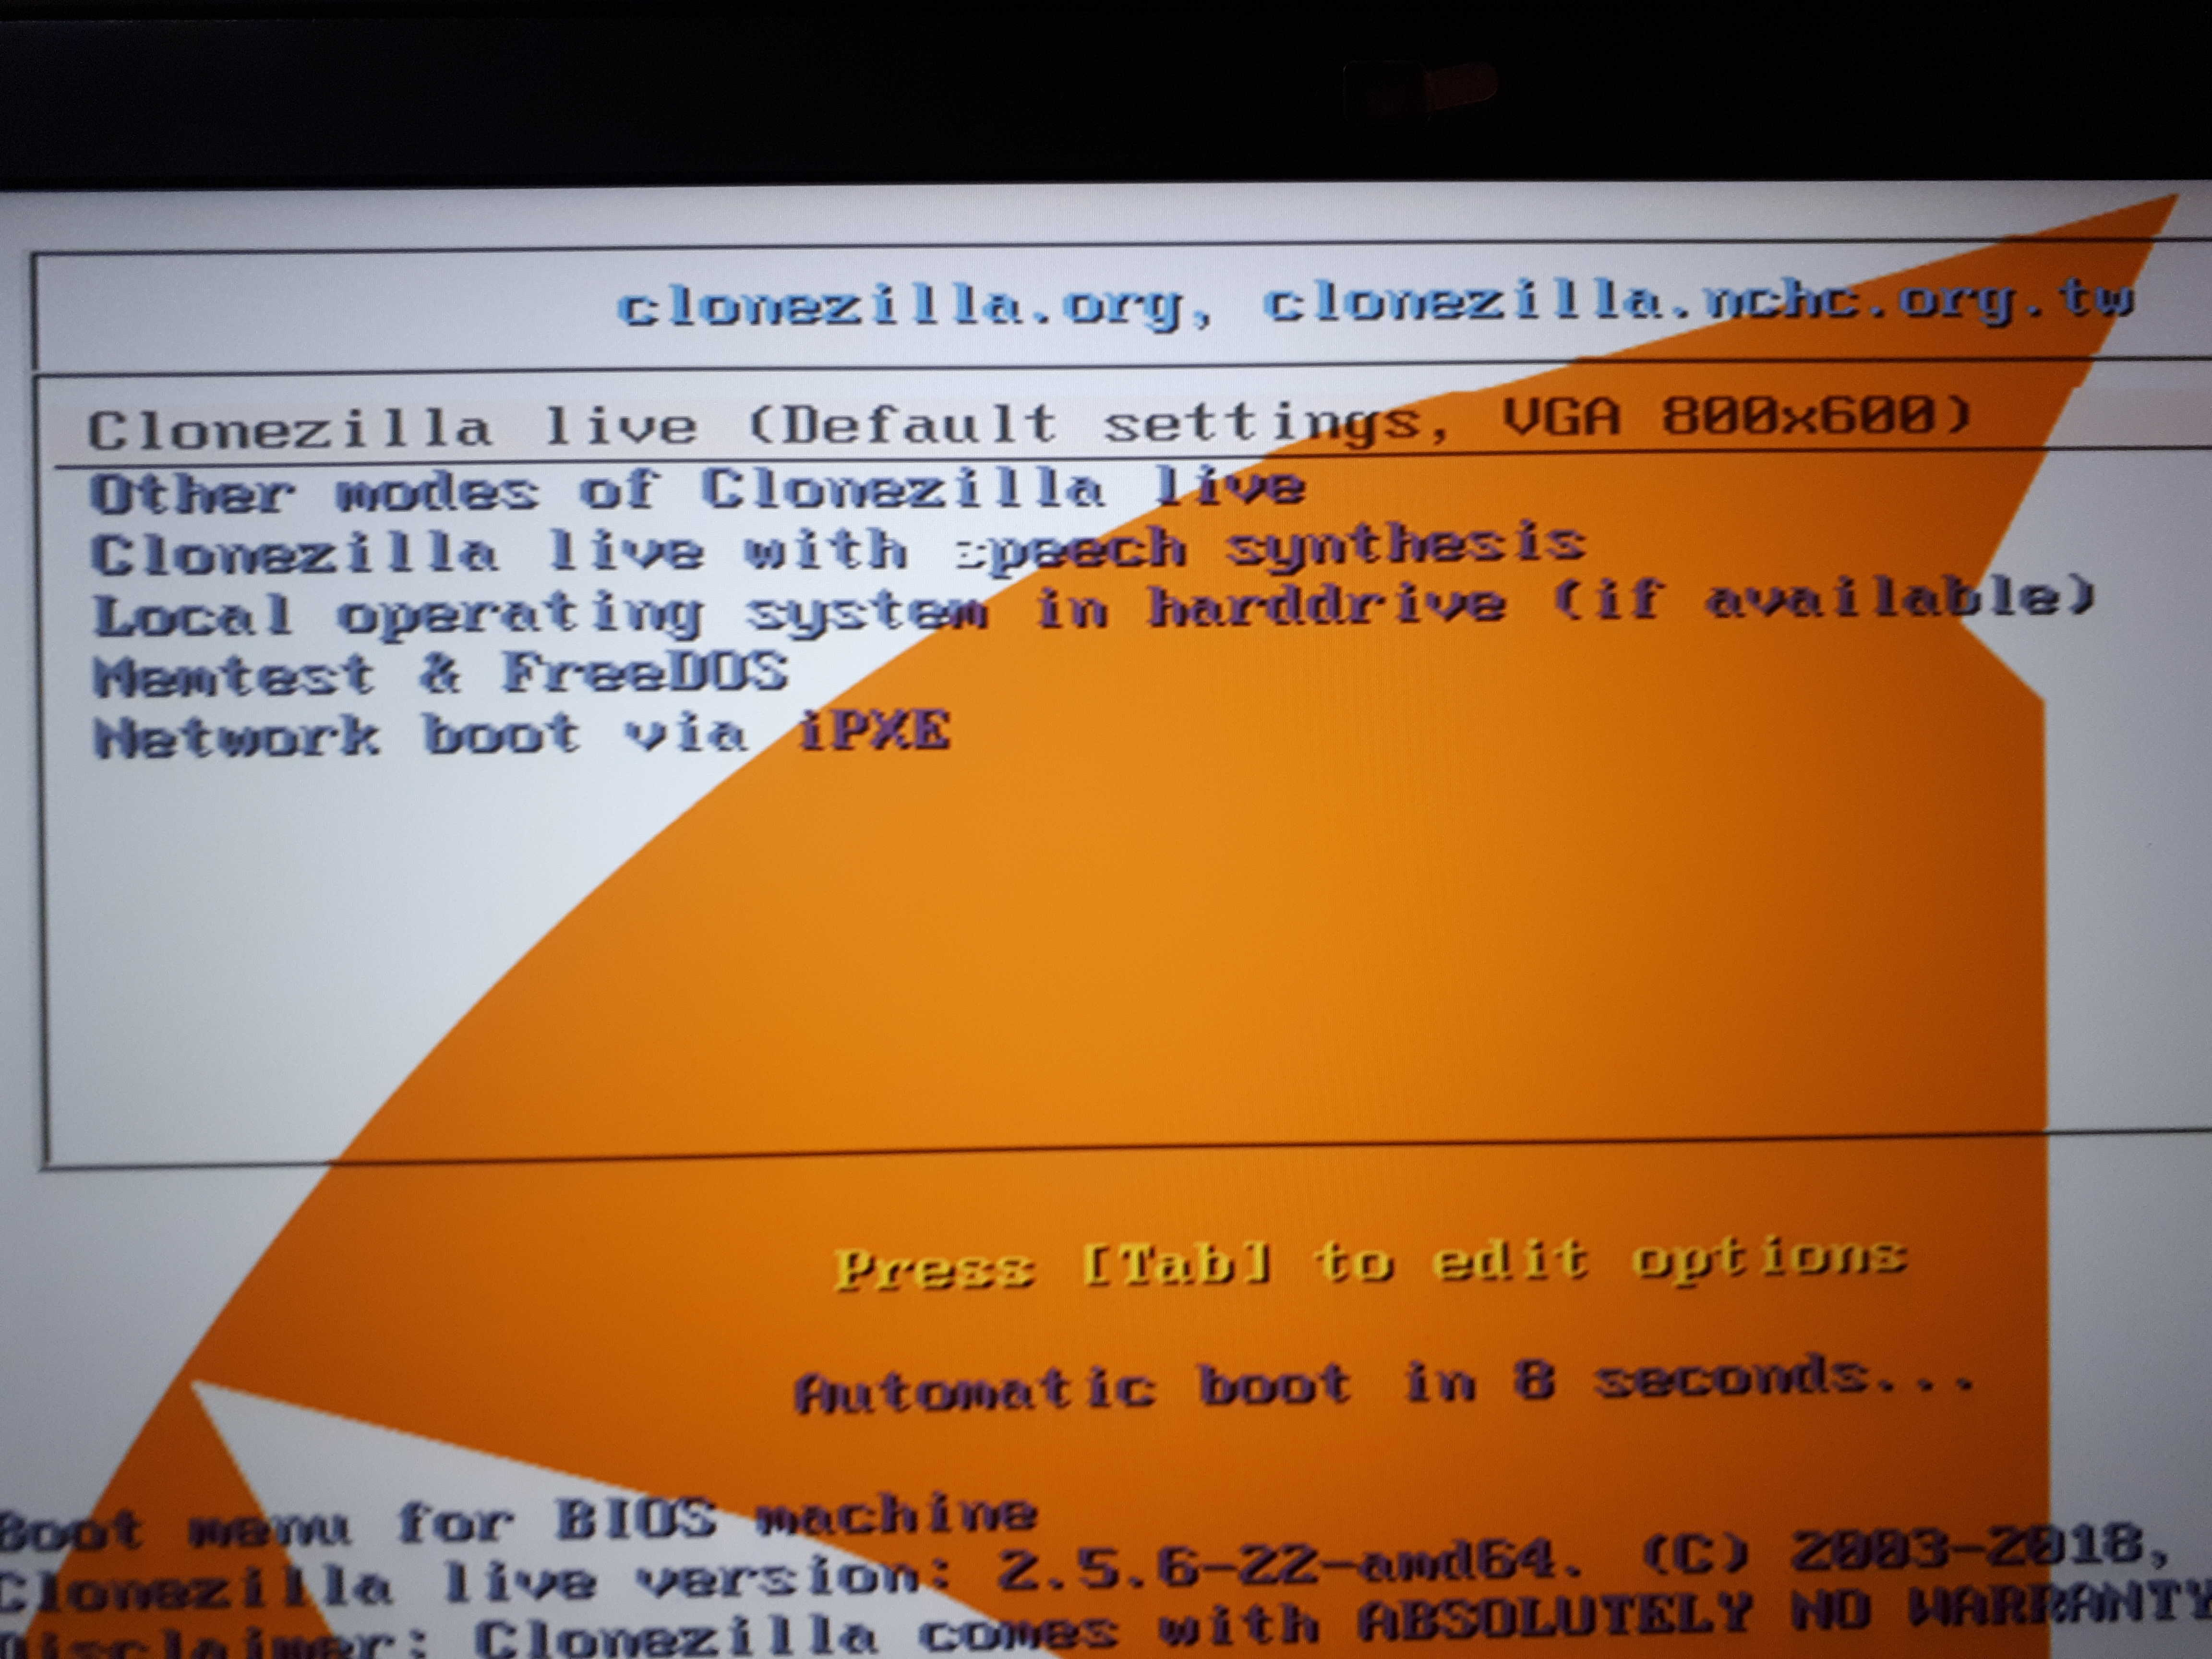
\includegraphics[width=1\linewidth]{images/backup/bkp2.jpg}
        \caption{Partições no Linux Programa GParted}
    \end{figure}
\end{frame}

\begin{frame}[plain,c]
   \frametitle{\insertsection}
    \framesubtitle{Escolhendo Idioma}
    \begin{figure}[!h]
        
        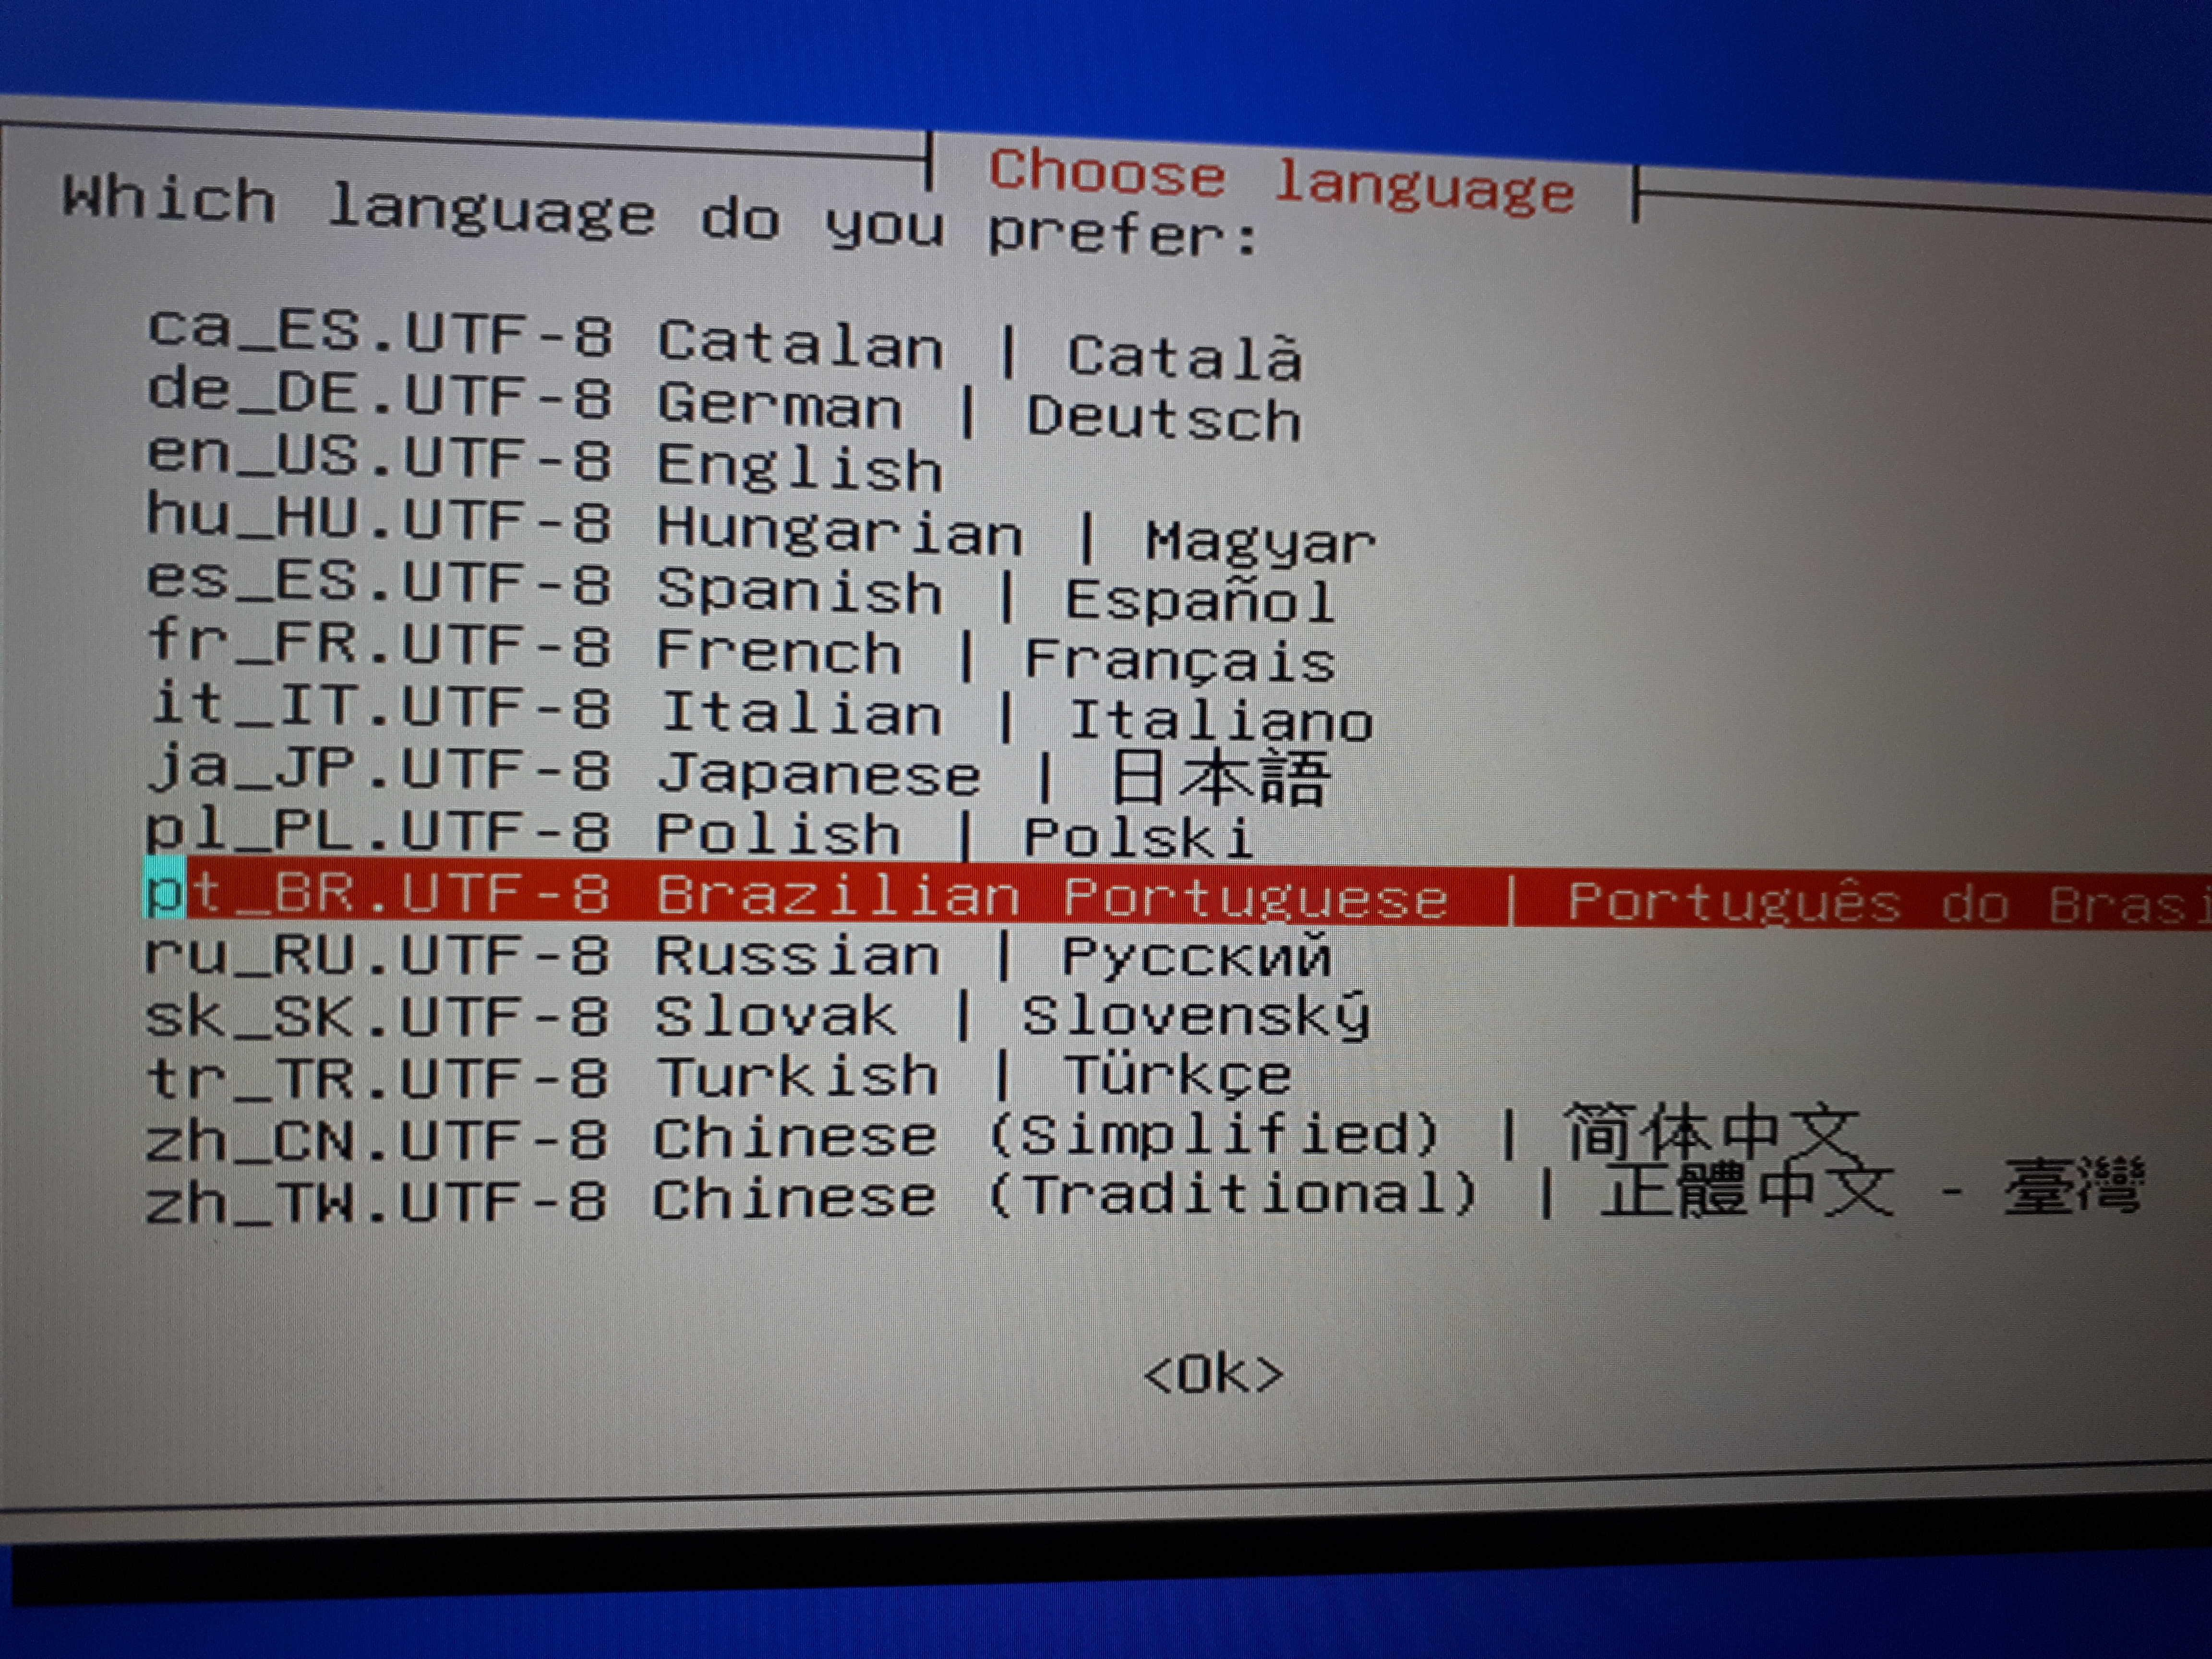
\includegraphics[width=1\linewidth]{images/backup/bkp3.jpg}
        \caption{Partições no Linux Programa GParted}
    \end{figure}
\end{frame}

\begin{frame}[plain,c]
   \frametitle{\insertsection}
    \framesubtitle{Layout do Teclado}
    \begin{figure}[!h]
        
        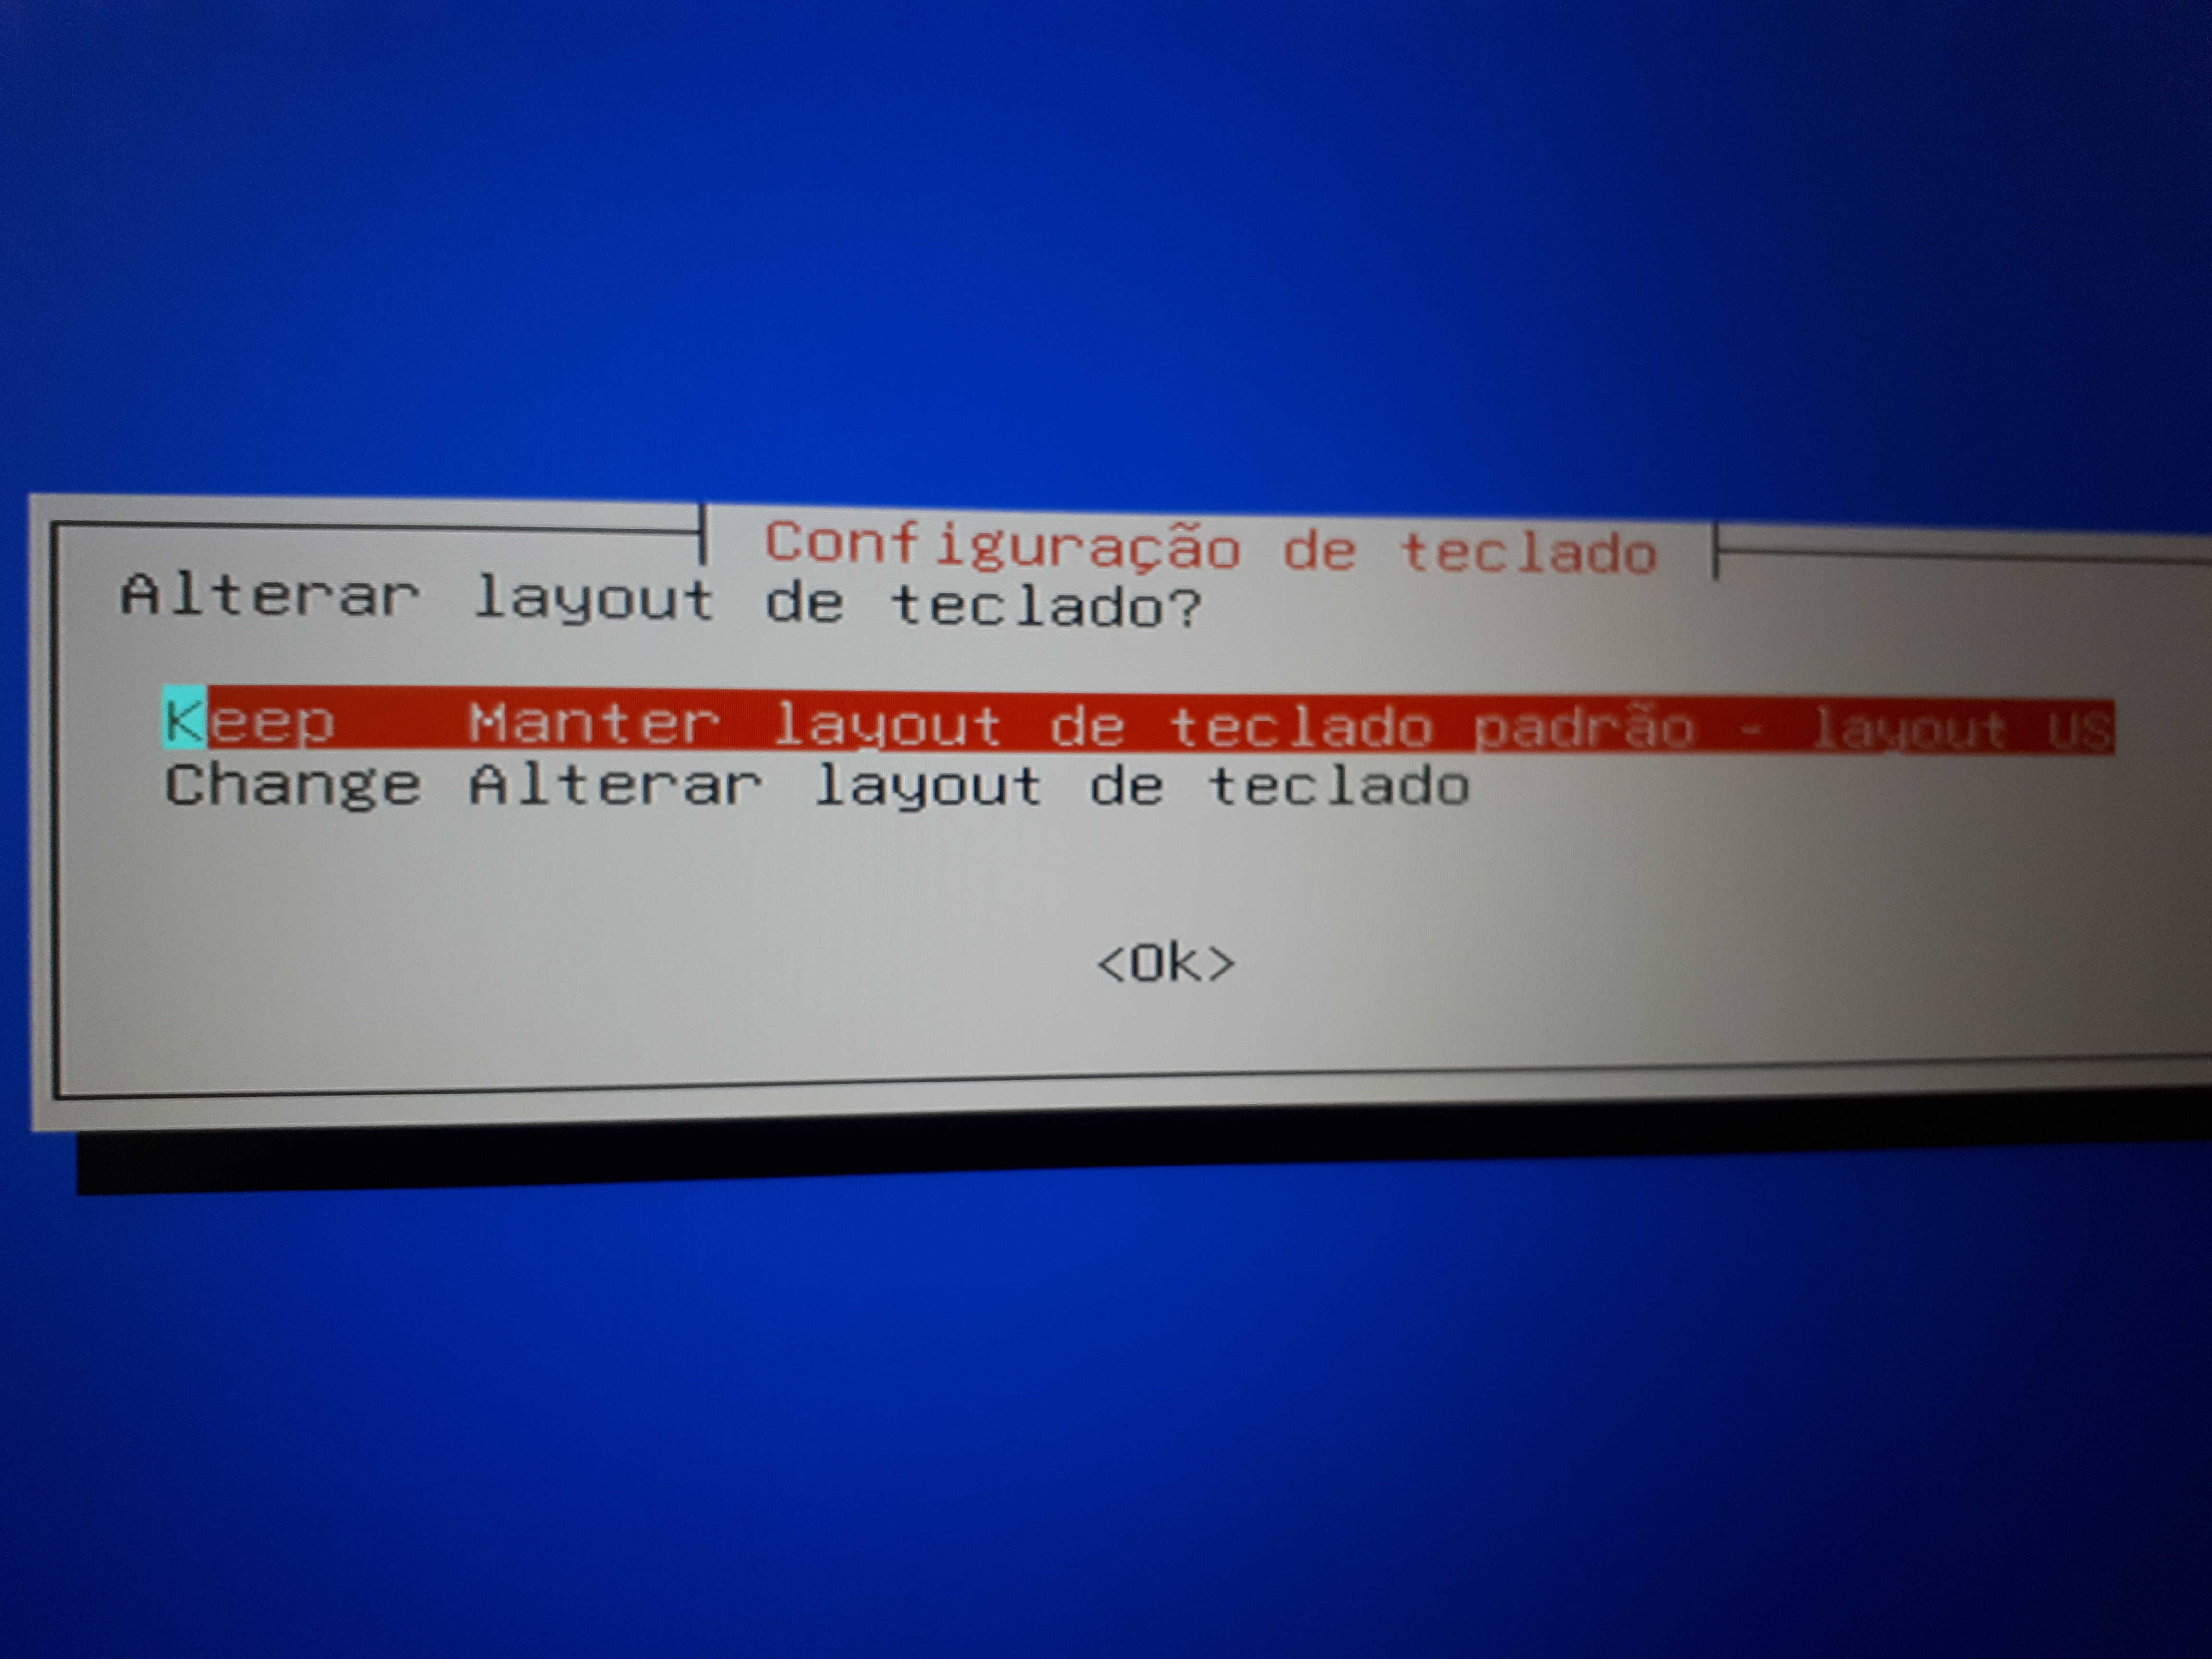
\includegraphics[width=1\linewidth]{images/backup/bkp4.jpg}
        \caption{Partições no Linux Programa GParted}
    \end{figure}
\end{frame}

\begin{frame}[plain,c]
   \frametitle{\insertsection}
    \framesubtitle{Iniciar CloneZilla}
    \begin{figure}[!h]
        
        \includegraphics[width=1\linewidth]{images/backup/bkp5.jpg}
        \caption{Partições no Linux Programa GParted}
    \end{figure}
\end{frame}

\begin{frame}[plain,c]
   \frametitle{\insertsection}
    \framesubtitle{Iniciar CloneZilla}
    \begin{figure}[!h]
        
        \includegraphics[width=1\linewidth]{images/backup/bkp5.jpg}
        \caption{Partições no Linux Programa GParted}
    \end{figure}
\end{frame}



\begin{frame}[plain,c]
   \frametitle{\insertsection}
    \framesubtitle{Escolher DISCO/PARTIÇÃO}
    \begin{figure}[!h]
        
        \includegraphics[width=1\linewidth]{images/backup/bkp6.jpg}
        \caption{Partições no Linux Programa GParted}
    \end{figure}
\end{frame}

\begin{frame}[plain,c]
   \frametitle{\insertsection}
    \framesubtitle{Localizar partição de DESTINO}
    \begin{figure}[!h]
        
        \includegraphics[width=1\linewidth]{images/backup/bkp7.jpg}
        \caption{Partições no Linux Programa GParted}
    \end{figure}
\end{frame}

\begin{frame}[plain,c]
   \frametitle{\insertsection}
    \framesubtitle{Para inserir HD Externo}
    \begin{figure}[!h]
        
        \includegraphics[width=1\linewidth]{images/backup/bkp8.jpg}
        \caption{Partições no Linux Programa GParted}
    \end{figure}
\end{frame}

\begin{frame}[plain,c]
   \frametitle{\insertsection}
    \framesubtitle{Todas os HDs disponíveis}
    \begin{figure}[!h]
        
        \includegraphics[width=1\linewidth]{images/backup/bkp9.jpg}
        \caption{Partições no Linux Programa GParted}
    \end{figure}
\end{frame}

\begin{frame}[plain,c]
   \frametitle{\insertsection}
    \framesubtitle{Escolhendo HD com IMAGENS}
    \begin{figure}[!h]
        \includegraphics[width=1\linewidth]{images/backup/bkp10.jpg}
        \caption{Partições no Linux Programa GParted}
    \end{figure}
\end{frame}

\begin{frame}[plain,c]
   \frametitle{\insertsection}
    \framesubtitle{Escolhendo Diretório no HD  com IMAGENS}
    \begin{figure}[!h]
        \includegraphics[width=1\linewidth]{images/rest/res1.jpg}
    \end{figure}
\end{frame}

\begin{frame}[plain,c]
   \frametitle{\insertsection}
    \framesubtitle{Escolhendo Diretório no HD com IMAGENS}
    \begin{figure}[!h]
        \includegraphics[width=1\linewidth]{images/rest/res2.jpg}
    \end{figure}
\end{frame}


\begin{frame}[plain,c]
   \frametitle{\insertsection}
    \framesubtitle{Escolhendo Diretório no HD com IMAGENS}
    \begin{figure}[!h]
        \includegraphics[width=1\linewidth]{images/rest/res3.jpg}
        \caption{Partições no Linux Programa GParted}
    \end{figure}
\end{frame}

\begin{frame}[plain,c]
   \frametitle{\insertsection}
    \framesubtitle{Escolher a opção RESTOREPARTS}
    \begin{figure}[!h]
        \includegraphics[width=1\linewidth]{images/rest/res4.jpg}
        \caption{Partições no Linux Programa GParted}
    \end{figure}
\end{frame}


\begin{frame}[plain,c]
   \frametitle{\insertsection}
    \framesubtitle{Escolher a opção RESTOREPARTS}
    \begin{figure}[!h]
        \includegraphics[width=1\linewidth]{images/rest/res5.jpg}
        \caption{Partições no Linux Programa GParted}
    \end{figure}
\end{frame}	

\begin{frame}[plain,c]
   \frametitle{\insertsection}
    \framesubtitle{SELECIONAR A IMAGEM}
    \begin{figure}[!h]
        \includegraphics[width=1\linewidth]{images/rest/res6.jpg}
        \caption{Partições no Linux Programa GParted}
    \end{figure}
\end{frame}	


\begin{frame}[plain,c]
   \frametitle{\insertsection}
    \framesubtitle{SELECIONAR A IMAGEM}
    \begin{figure}[!h]
        \includegraphics[width=1\linewidth]{images/rest/res7.jpg}
        \caption{Partições no Linux Programa GParted}
    \end{figure}
\end{frame}	


\begin{frame}[plain,c]
   \frametitle{\insertsection}
    \framesubtitle{SELECIONAR A IMAGEM}
    \begin{figure}[!h]
        \includegraphics[width=1\linewidth]{images/rest/res8.jpg}
        \caption{Partições no Linux Programa GParted}
    \end{figure}
\end{frame}	

\begin{frame}[plain,c]
   \frametitle{\insertsection}
    \framesubtitle{SELECIONAR A IMAGEM}
    \begin{figure}[!h]
        \includegraphics[width=1\linewidth]{images/rest/res9.jpg}
        \caption{Partições no Linux Programa GParted}
    \end{figure}
\end{frame}	


\begin{frame}[plain,c]
   \frametitle{\insertsection}
    \framesubtitle{SELECIONAR A IMAGEM}
    \begin{figure}[!h]
        \includegraphics[width=1\linewidth]{images/rest/res10.jpg}
        \caption{Partições no Linux Programa GParted}
    \end{figure}
\end{frame}	


\begin{frame}[plain,c]
   \frametitle{\insertsection}
    \framesubtitle{SELECIONAR A IMAGEM}
    \begin{figure}[!h]
        \includegraphics[width=1\linewidth]{images/rest/res11.jpg}
        \caption{Partições no Linux Programa GParted}
    \end{figure}
\end{frame}

\begin{frame}[plain,c]
   \frametitle{\insertsection}
    \framesubtitle{SELECIONAR A PARTIÇÃO DE DESTINO}
    \begin{figure}[!h]
        \includegraphics[width=1\linewidth]{images/rest/res12.jpg}
        \caption{Partições no Linux Programa GParted}
    \end{figure}
\end{frame}	

\begin{frame}[plain,c]
   \frametitle{\insertsection}
    \framesubtitle{SELECIONAR A PARTIÇÃO DE DESTINO}
    \begin{figure}[!h]
        \includegraphics[width=1\linewidth]{images/rest/res13.jpg}
        \caption{Partições no Linux Programa GParted}
    \end{figure}
\end{frame}	

\begin{frame}[plain,c]
   \frametitle{\insertsection}
    \framesubtitle{Verificar a IMAGEM antes de Restaurar}
    \begin{figure}[!h]
        \includegraphics[width=1\linewidth]{images/rest/res14.jpg}
        \caption{Partições no Linux Programa GParted}
    \end{figure}
\end{frame}	
	
	
\begin{frame}[plain,c]
   \frametitle{\insertsection}
    \framesubtitle{Escolher o que fazer quando terminar o processo.}
    \begin{figure}[!h]
        \includegraphics[width=1\linewidth]{images/rest/res15.jpg}
        \caption{Partições no Linux Programa GParted}
    \end{figure}
\end{frame}	
	
\begin{frame}[plain,c]
   \frametitle{\insertsection}
    \framesubtitle{Verificando as imagens.}
    \begin{figure}[!h]
        \includegraphics[width=1\linewidth]{images/rest/res16.jpg}
        \caption{Partições no Linux Programa GParted}
    \end{figure}
\end{frame}		

	
\begin{frame}[plain,c]
   \frametitle{\insertsection}
    \framesubtitle{Verificando as imagens.}
    \begin{figure}[!h]
        \includegraphics[width=1\linewidth]{images/rest/res17.jpg}
        \caption{Partições no Linux Programa GParted}
    \end{figure}
\end{frame}		

\begin{frame}[plain,c]
   \frametitle{\insertsection}
    \framesubtitle{Confirmação de que as IMAGENS são RESTAURÁVEIS.}
    \begin{figure}[!h]
        \includegraphics[width=1\linewidth]{images/rest/res18.jpg}
        \caption{Partições no Linux Programa GParted}
    \end{figure}
\end{frame}

\begin{frame}[plain,c]
   \frametitle{\insertsection}
    \framesubtitle{CONFIRMAÇÃO PARA PROSSEGUIR COM A RESTAURAÇÃO DA PARTIÇÃO.}
    \begin{figure}[!h]
        \includegraphics[width=1\linewidth]{images/rest/res19.jpg}
        \caption{Partições no Linux Programa GParted}
    \end{figure}
\end{frame}

\begin{frame}[plain,c]
   \frametitle{\insertsection}
    \framesubtitle{INÍCIO DO PROCESSO DE RESTAURAÇÃO.}
    \begin{figure}[!h]
        \includegraphics[width=1\linewidth]{images/rest/res20.jpg}
        \caption{Partições no Linux Programa GParted}
    \end{figure}
\end{frame}

\begin{frame}[plain,c]
   \frametitle{\insertsection}
    \framesubtitle{PROCESSO DE RESTAURAÇÃO FINALIZADO.}
    \begin{figure}[!h]
        \includegraphics[width=1\linewidth]{images/rest/res21.jpg}
        \caption{Partições no Linux Programa GParted}
    \end{figure}
\end{frame}

\begin{frame}[plain,c]
   \frametitle{\insertsection}
    \framesubtitle{OPÇÕES FINAIS.}
    \begin{figure}[!h]
        \includegraphics[width=1\linewidth]{images/rest/res22.jpg}
        \caption{Partições no Linux Programa GParted}
    \end{figure}
\end{frame}
		
\appendix

%\begin{frame}[allowframebreaks]{References}
%    \tiny
%    \bibliography{bib}
%    \bibliographystyle{plainnat}
%\end{frame}

\begin{frame}[plain,c]
\vspace{2.5cm}
    \begin{center}
      \Huge \textbf{MUITO OBRIGADO !}\\
      \Huge \textbf{;)}\\  
      \medskip
      \medskip
      \medskip
      \medskip
      \medskip
      \small \textbf{VISITE:}\\
      \small \href{http://www.ifsul.edu.br}{IFSUL}\\
      \small\href{https://tchelinux.org/}{TCHELINUX}\\
      \small\href{https://clonezilla.org/}{CLONEZILLA}\\
    \end{center}
\end{frame}

\end{document}
